% !Mode:: "Tex:UTF-8"

\section{Variables correlacionadas y funciones.}
\label{cap10:sec:VariablesCorrelacionadasFunciones}

En este capítulo vamos a investigar la relación que, en la introducción a esta parte del curso,
hemos llamado C $\sim$ C, entre dos variables cuantitativas. Muchas leyes científicas, relacionadas
con procesos físicos o químicos se expresan en esta forma, como hemos dicho. Por ejemplo, en el
artículo \cite{haftorn1985effect}, los investigadores (S. Haftorn, R. E. Reinertsen) estudian
(entre otras cosas) la relación entre el consumo de oxígeno y la temperatura del aire en una hembra de {\em Herrerillo Común} ({\em Parus Caeruleus}, el ave que puedes ver en la Figura
\ref{cap10:fig:Herrerillo}. Ver enlace [\,\ref{enlace0020}\,]\label{enlace0020a} de la Wikipedia), tanto cuando está incubando, como cuando no lo está.

\begin{figure}[htbp]
\begin{center}
\begin{enColor}

\includegraphics[width=11cm]{../fig/Cap10-Herrerillo.png}
\end{enColor}
\begin{bn}

\includegraphics[width=11cm]{../fig/Cap10-Herrerillo-bn.png}
\end{bn}
\caption{Un {\em Herrerillo Común (Parus Caeruleus)}, observado cerca de Madrid.}
\label{cap10:fig:Herrerillo}
\end{center}
\end{figure}

A los investigadores, en situaciones como esta, les interesa estudiar si hay alguna relación entre ambas variables. Al pensar un poco sobre este problema, podemos sospechar que, a menor temperatura, mayor consumo de oxígeno. Cuanto más frío hace, más oxígeno tiene que ``quemar'' la hembra de {\em Herrerillo} para mantenerse, a sí misma y a la puesta, calientes. Conceptualmente, podemos representar esta idea como hemos hecho en la Figura \ref{cap10:fig:Herrerillo02}.

\begin{figure}[htbp]
\begin{center}
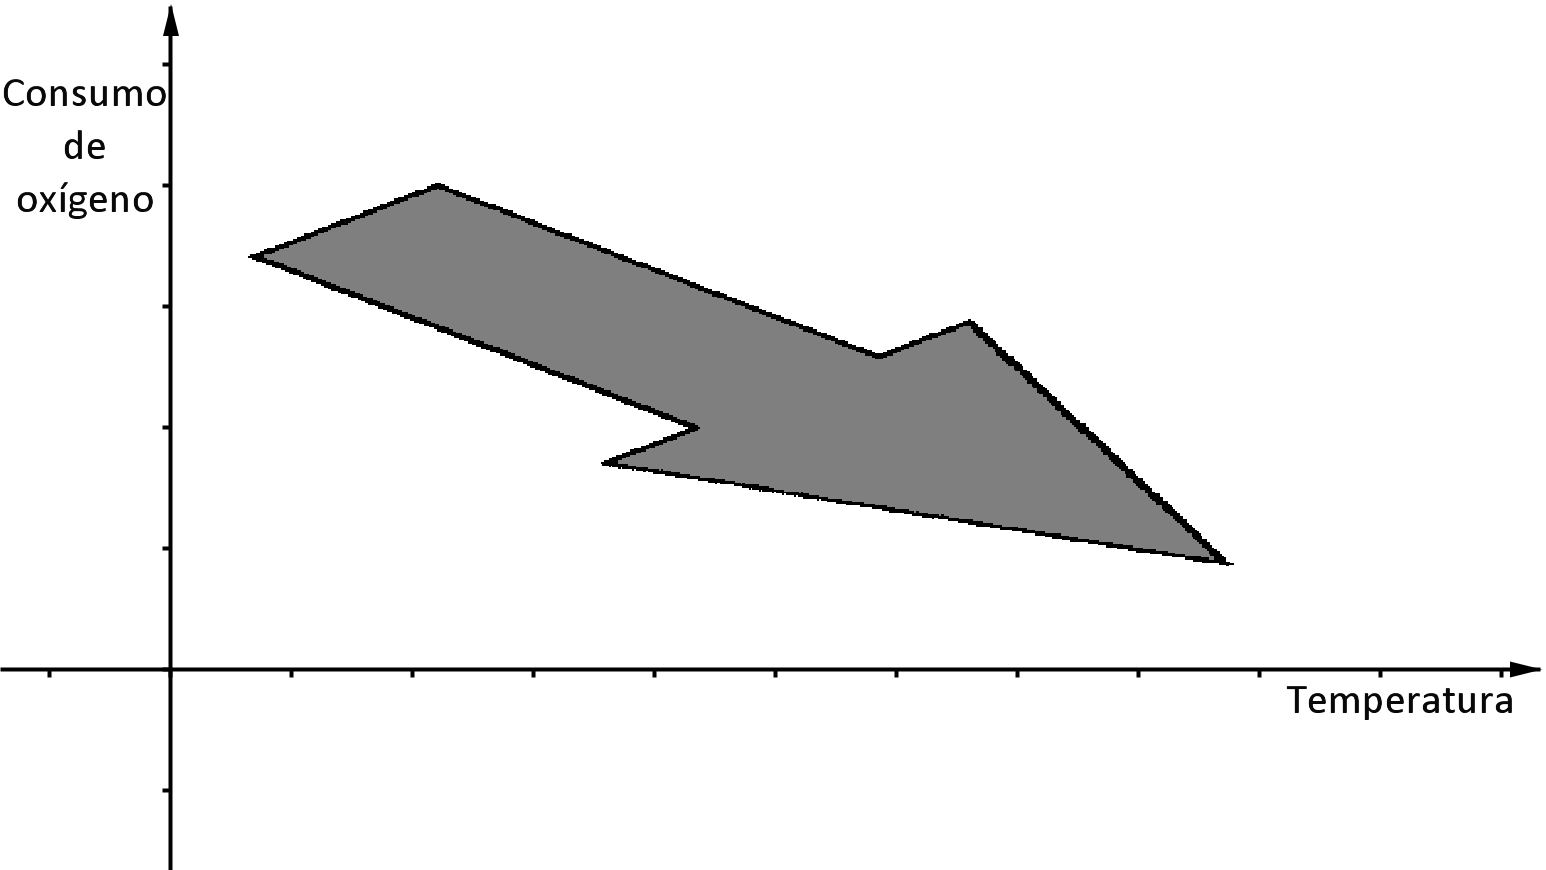
\includegraphics[width=13cm]{../fig/Cap10-IntuicionProblemaHerrerillos.png}
\caption{Nuestra intuición sobre la relación entre las dos variables en el problema de los herrerillos.}
\label{cap10:fig:Herrerillo02}
\end{center}
\end{figure}

La figura refleja esa intuición de que a temperaturas más bajas les corresponden consumos de oxígeno más altos. La idea de {\sf correlación}\index{correlación} se corresponde con este tipo de situaciones donde hay un vínculo de cierto tipo entre los valores de dos variables. La correlación está íntimamente relacionada con la idea de independencia, claro. Uno de nuestros objetivos en este capítulo es profundizar en la idea de correlación, aclarar qué tiene que ver la correlación con la independencia, y con otro concepto, el de {\sf causalidad}\index{causalidad},  con el que a menudo se confunde. Para hacer todo esto tendremos que dar una definición mucho más precisa de la correlación.

Y tenemos que hacer eso, porque desde luego, querríamos disponer de una herramienta más precisa que la mera {\em intuición} que hay detrás de la Figura \ref{cap10:fig:Herrerillo02}. Algo que nos permitiera hacer {\em predicciones}. Algo como una {\em fórmula}, en la que introducir la temperatura del aire, y poder calcular el consumo de oxígeno. No se trata de hacer muchas, muchísimas medidas hasta tener cubiertas todas las temperaturas posibles, sino de usar las medidas que tenemos para establecer la relación entre esas dos variables.

El objetivo de una fórmula como esa es cumplir una de las tareas esenciales de los modelos
científicos: la {\sf predicción}.  Es decir, que, una vez que tengamos esa fórmula
    \[y=f(x),\]
nuestro plan es que, cada vez que obtengamos un valor de la variable $x$ podremos utilizar esta
ecuación para {\sf predecir el valor de $y$ sin necesidad de medirlo}. Y esto es muy interesante
porque, en muchos  casos, habrá una variable $x$ {\em fácil} de medir, mientras que la medición de
$y$ puede ser muy complicada. En el ejemplo de la hembra de {\em Herrerillo} incubando, es muy fácil medir la temperatura del aire en un día concreto, basta con usar un termómetro, que interfiere muy poco en la vida del ave, por lo que esa medida perturba muy poco los restantes parámetros del experimento. En cambio, medir el consumo de oxígeno del pobre pajarillo obliga a colocarle, de alguna manera, al alcance de algún tipo de aparato de medida (recomendamos leer el dispositivo experimental utilizado por los autores del artículo que estamos utilizando como referencia, para ver, entre otras cosas, porque han elegido al {\em Herrerillo} para este estudio). Ese tipo de operaciones no sólo son complejas y muy laboriosas, sino que debe realizarse concienzudamente, poniendo mucho esmero para que el propio diseño  experimental no perturbe los mismos parámetros que estamos tratando de medir. Así que, en un ejemplo como este, la variable $x$ sería la temperatura del aire, la variable $y$ sería el consumo de oxígeno y querríamos una fórmula $y=f(x)$ que nos permita predecir el consumo de oxígeno a partir de la lectura del termómetro. En ese tipo de situaciones diremos que $x$ es la {\sf variable independiente}\index{variable independiente}, {\sf variable predictora}\index{variable predictora}, o {\sf regresora}\index{variable regresora}, mientras que $y$ es la {\sf variable dependiente} o {\sf respuesta}\index{variable respuesta}\index{respuesta, variable.}.

La idea de fórmula $y=f(x)$ se traduce habitualmente, en el lenguaje de las matemáticas, en una función
\[y=f(x),\]
de las que el lector conoce numerosos ejemplos: funciones polinómicas, funciones
racionales (cocientes de polinomios), exponenciales (como $f(x)=e^x$), logaritmos, trigonométricas
(seno, coseno), y otras muchas, más o menos complicadas. Cada una de esas funciones, como por
ejemplo, la función racional
    \[y=\frac{x}{x^2+1}.\]
    %    \[y=f(x)=x^2/(1+x^4)\]
que hemos visto en la introducción a esta parte del curso, representa una relación exacta entre las variables $x$ e $y$, que a cada valor de la $x$ le hace corresponder un valor (y uno sólo) de la $y$. Nos gusta pensar siempre en el ejemplo de los botones de una calculadora. Tecleo un número $x$, por ejemplo $4$, pulso el botón de función, por ejemplo el de raíz cuadrada, y obtengo un valor de $y$, en este caso $2$.

Este tipo de relaciones exactas se utilizan, en las aplicaciones de las matemáticas, como modelos teóricos. El modelo clásico son las leyes de la Física, como las leyes de Newton, Maxwell, etcétera. Si queremos calcular la fuerza de atracción gravitatoria $F$ entre dos cuerpos de masas $m_1$ y $m_2$, situados a distancia $r$, sabemos que, con las unidades correctas, esta fuerza viene dada por la ley de Newton:
        \[F(r)=G\,\dfrac{m_1\cdot m_2}{r^2}\]
($G$ es la constante de gravitación universal). Es decir, que sustituimos aquí un valor de $r$ y obtenemos un valor de $F$, en principio (teóricamente) con toda la precisión que queramos. Pero, claro está, esa visión es un {\em modelo teórico}. Cuando vayamos al mundo real y tratemos de aplicar esta fórmula, por ejemplo a  la atracción gravitatoria entre la Tierra y la Luna, surgen muchos matices que debemos tener en cuenta:
        \begin{enumerate}
            \item Ni las masas, ni las distancias, se pueden medir con una precisión infinita.
               Y no es sólo porque haya errores experimentales de medida, es que además hay
                límites teóricos a la precisión de las medidas, como el {\em Principio de incertidumbre} de la Mecánica Cuántica.
            \item Incluso aceptando como correctas las leyes de Newton, para plantear el modelo
                estamos introduciendo muchas simplificaciones e idealizaciones. Por ejemplo,  estamos considerando que esos dos cuerpos que se atraen se pueden considerar como partículas puntuales (idealización). Y estamos ignorando la presencia de otros cuerpos (simplificación)
            \item Y además, ahora sabemos que la ley de la gravedad de Newton sólo es precisa
                dentro de un determinado intervalo de valores de los parámetros. Para escalas
                espaciales muy grandes o muy pequeñas, o para objetos enormemente masivos
                (agujeros negros, por ejemplo) o extremadamente ligeros (partículas
                subatómicas), sus predicciones son incorrectas, y tenemos que usar las
                correcciones que hizo Einstein, o las últimas teorías de gravedad cuántica, si
                queremos resultados muy precisos.
        \end{enumerate}

Por (entre otras) estas razones, sabemos que estas leyes son modelos teóricos, y no
esperamos que sus predicciones se cumplan con precisión absoluta. Ni siquiera lo
esperábamos cuando el modelo predominante en ciencia era el determinismo de Newton y
Laplace.
%(nota al final, pág. \pageref{sec:notaSobreDeterminismo})
No es realista esperar que las observaciones se correspondan exactamente con un modelo
teórico como el que refleja una ecuación del tipo $y=f(x)$. En el caso de la Biología,
que estudia fenómenos y procesos muy complejos, a menudo no es posible aislar las variables bajo estudio de su entorno, sin perturbar irremediablemente el propio objeto de estudio.
Así que tenemos que aceptar como un hecho que la relación entre variables, en Biología,
a menudo no es tan nítida como puede suceder con otros ejemplos de la Física o la Química.


\subsection{Diagramas de dispersión y la elección de la función adecuada.}
\label{cap10:subsec:DiagramasDIspersionEleccionFuncionAdecuada}

Volvamos al problema de los herrerillos. Los investigadores, laboriosa y concienzudamente han ido obteniendo medidas de  las dos variables bajo estudio. Y es esencial entender que lo que se mide son {\sf pares} de valores, medidos a la vez; de manera que el resultado del experimento es una lista o tabla de parejas de números.
\[(x_1,y_1),(x_2,y_2),(x_3,y_3),\ldots,(x_n,y_n),\]
(se habla a veces de una {\sf nube de puntos}\index{nube de puntos}), donde cada uno de los datos corresponde a una de las dos variables, $X$ para la coordenada
horizontal, e $Y$ para la coordenada vertical.  En este ejemplo $X$ representa la temperatura del
aire, e $Y$ el consumo de oxígeno,

El primer paso, una vez recopilados los datos, debe ser, como siempre, descriptivo. También podemos decir {\em exploratorio}. ¿Qué aspecto tienen los datos?  Para explorar los datos de tipo $(x,y)$ empezamos por representarlos en un plano de coordenadas, en lo que se conoce como {\sf diagrama de dispersión}\index{diagrama de dispersión}\index{dispersión, diagrama de} (en inglés, {\em scatter plot}\index{scatter plot}). Para el ejemplo de los herrerillos, ese diagrama podría tener el aspecto que se muestra en la Figura \ref{cap10:fig:Herrerillo01} (los datos de esa figura son simulados). Esta figura puede verse como una primera confirmación experimental de la intuición que había detrás de la Figura \ref{cap10:fig:Herrerillo02}. En el Tutorial10 aprenderemos a fabricar estos diagramas, de dispersión y otras gráficas que vamos a necesitar, utilizando distintos programas.

El diagrama de dispersión no tiene, sin embargo, la capacidad predictiva que andamos buscando. Para eso, como hemos argumentado, debemos tratar de encontrar una fórmula que encaje bien con los datos de esa figura.

\begin{figure}[t]
\begin{center}
\begin{enColor}
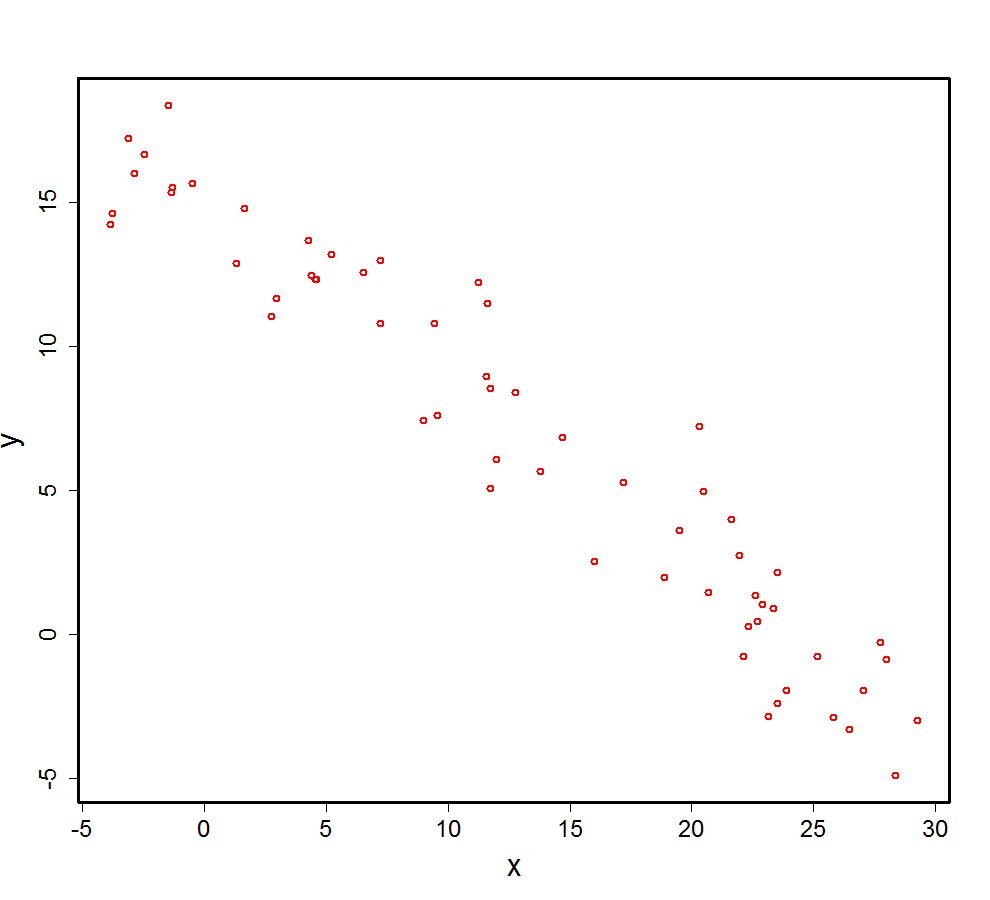
\includegraphics[width=11cm]{../fig/Cap10-GraficoDispersionHerrerilloSimulado.png}
\end{enColor}
\begin{bn}
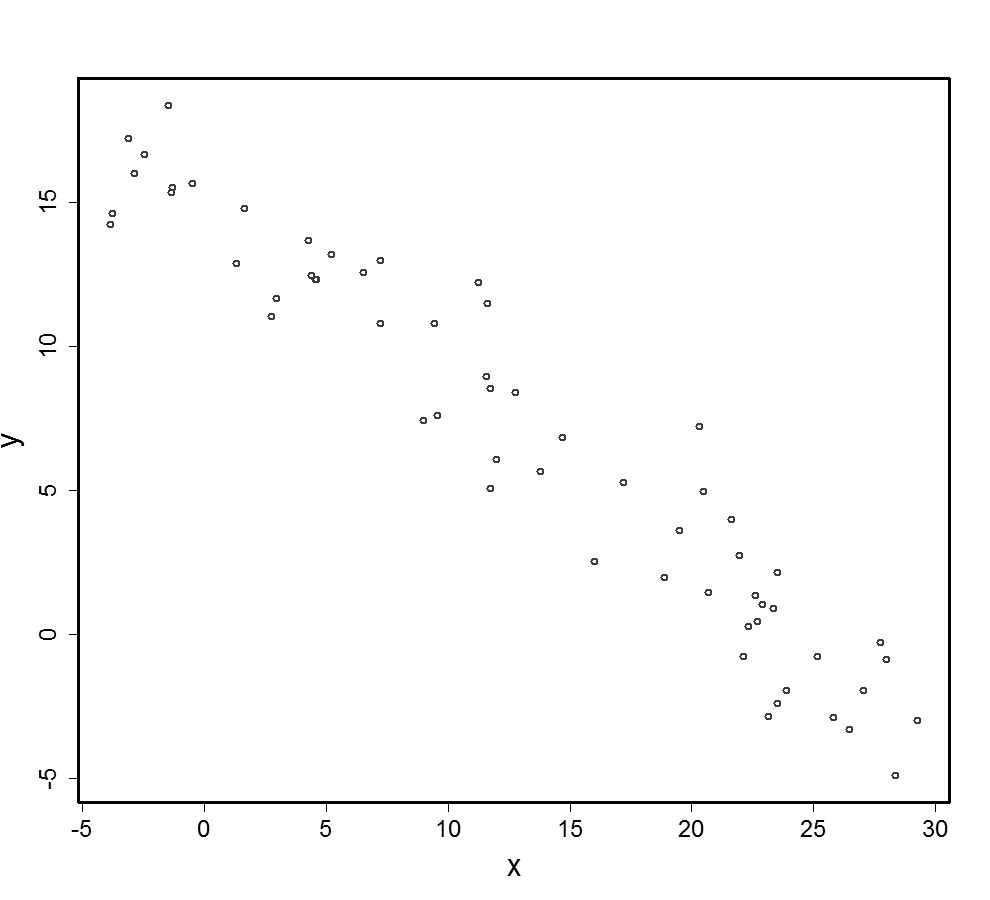
\includegraphics[width=11cm]{../fig/Cap10-GraficoDispersionHerrerilloSimulado-bn.png}
\end{bn}
\caption{Diagrama de dispersión (con datos simulados) para el experimento del {\em Herrerillo} incubando. El eje $x$ representa la temperatura y el eje $y$ el consumo de oxígeno, en las unidades adecuadas.}
\label{cap10:fig:Herrerillo01}
\end{center}
\end{figure}

Naturalmente, fórmulas (es decir, funciones) hay muchas... y los matemáticos saben fabricar fórmulas distintas para distintas necesidades. Por ejemplo, usando un procedimiento que se llama {\sf interpolación}, podemos fabricar un polinomio que pase por todos y cada uno de los puntos\footnote{Hay un detalle técnico: no debe haber dos puntos con la misma coordenada $x$}. Es decir, que si tenemos los cuatro puntos $A, B, C, D$ de la Figura \ref{cap10:fig:Interpolacion01}(a), para los matemáticos es sencillo encontrar un polinomio (de grado tres, al ser cuatro los puntos) que pase por todos ellos, como en la Figura \ref{cap10:fig:Interpolacion01}(b). Concretamente, para ese ejemplo el polinomio que hemos obtenido es este:
\[y=f(x)=0.33x^3-4.18x^2+16.3x-16.52.\]

\begin{figure}[htbp]
\begin{center}
\begin{enColor}
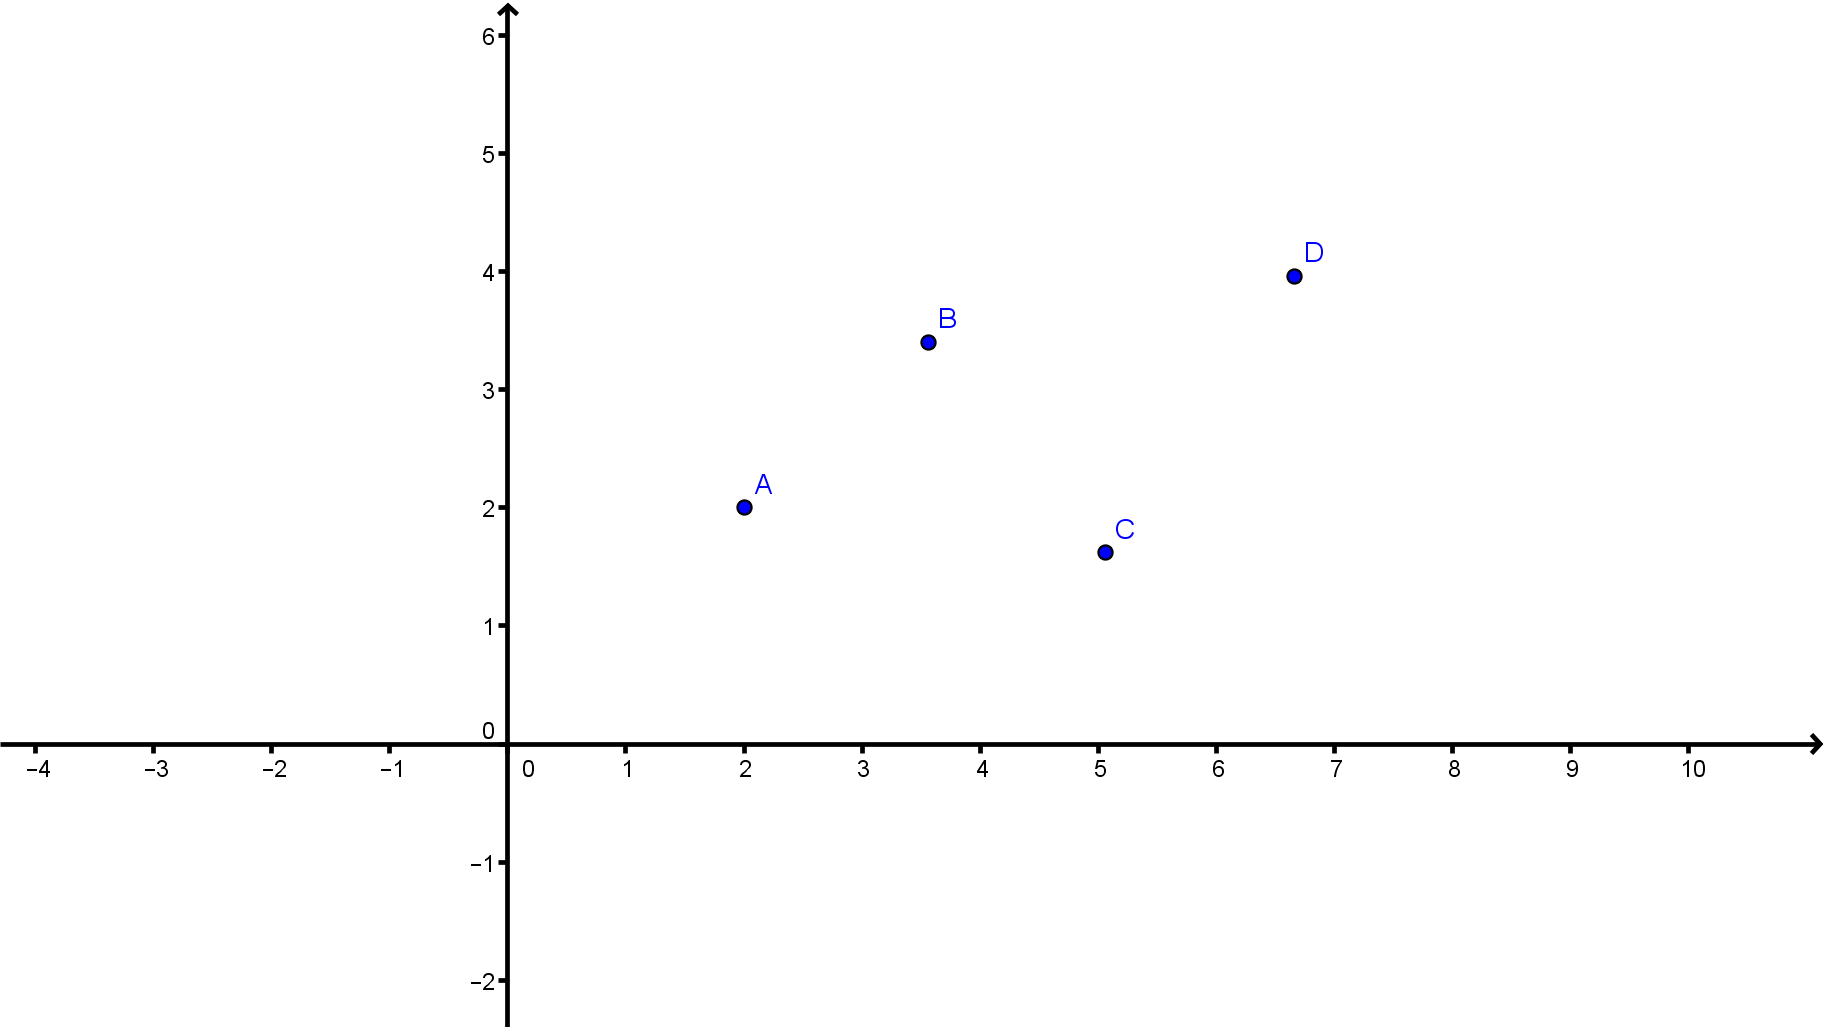
\includegraphics[width=12cm]{../fig/Cap10-Interpolacion01.png}\\
(a) Buscamos una f\'ormula que explique estos cuatro puntos.\\[3mm]
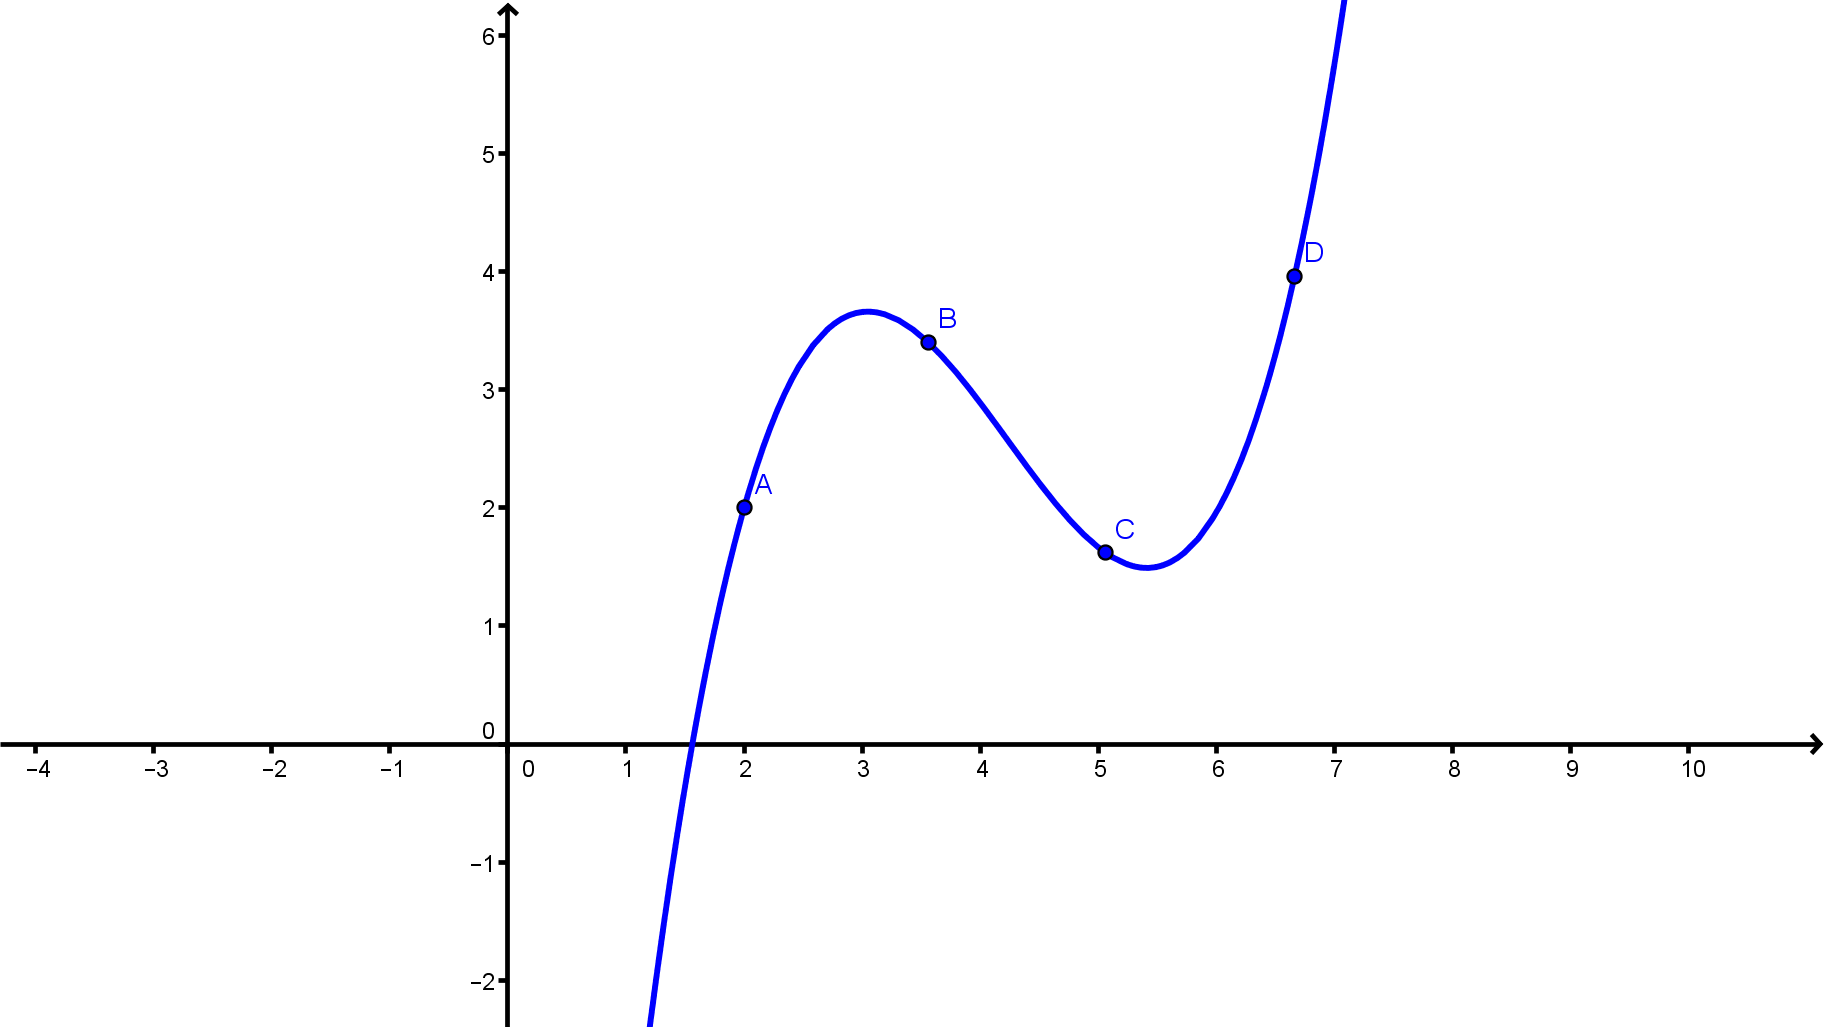
\includegraphics[width=12cm]{../fig/Cap10-Interpolacion02.png}\\
(b) El polinomio de grado tres que pasa por esos cuatro puntos.
\end{enColor}
\begin{bn}
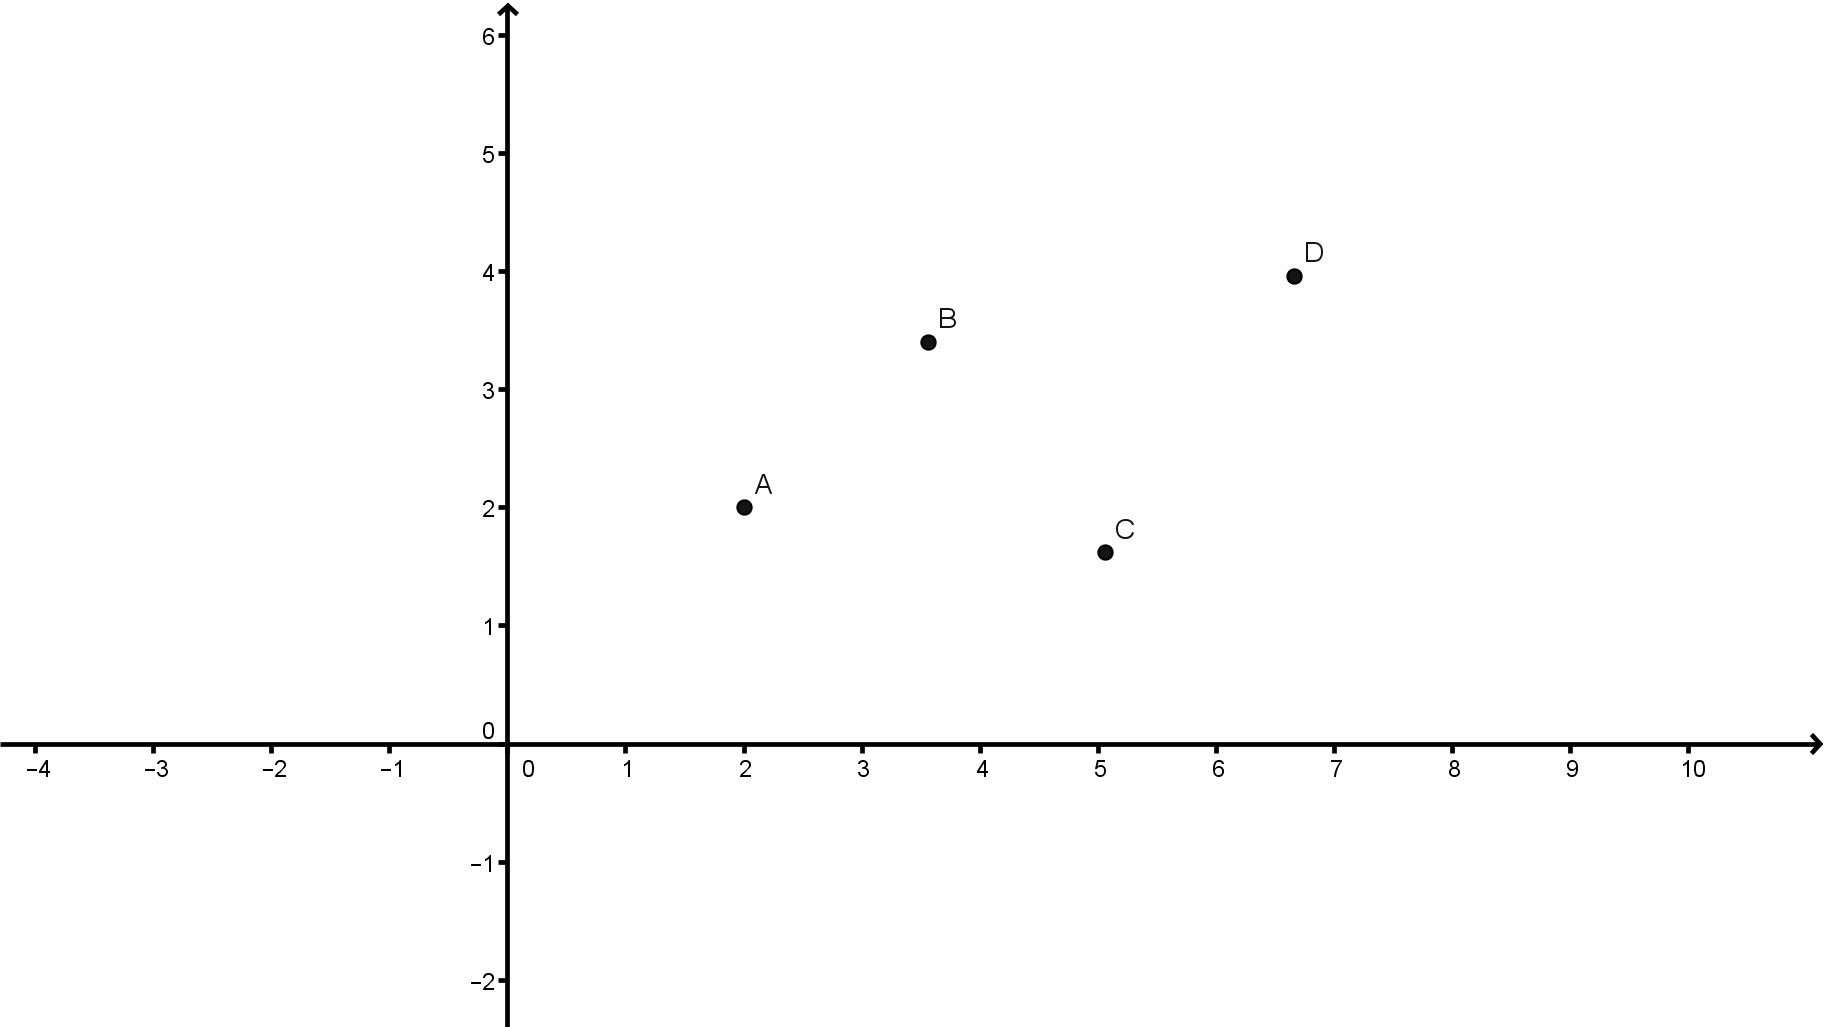
\includegraphics[width=12cm]{../fig/Cap10-Interpolacion01-bn.png}\\
(a) Buscamos una f\'ormula que explique estos cuatro puntos.\\[3mm]
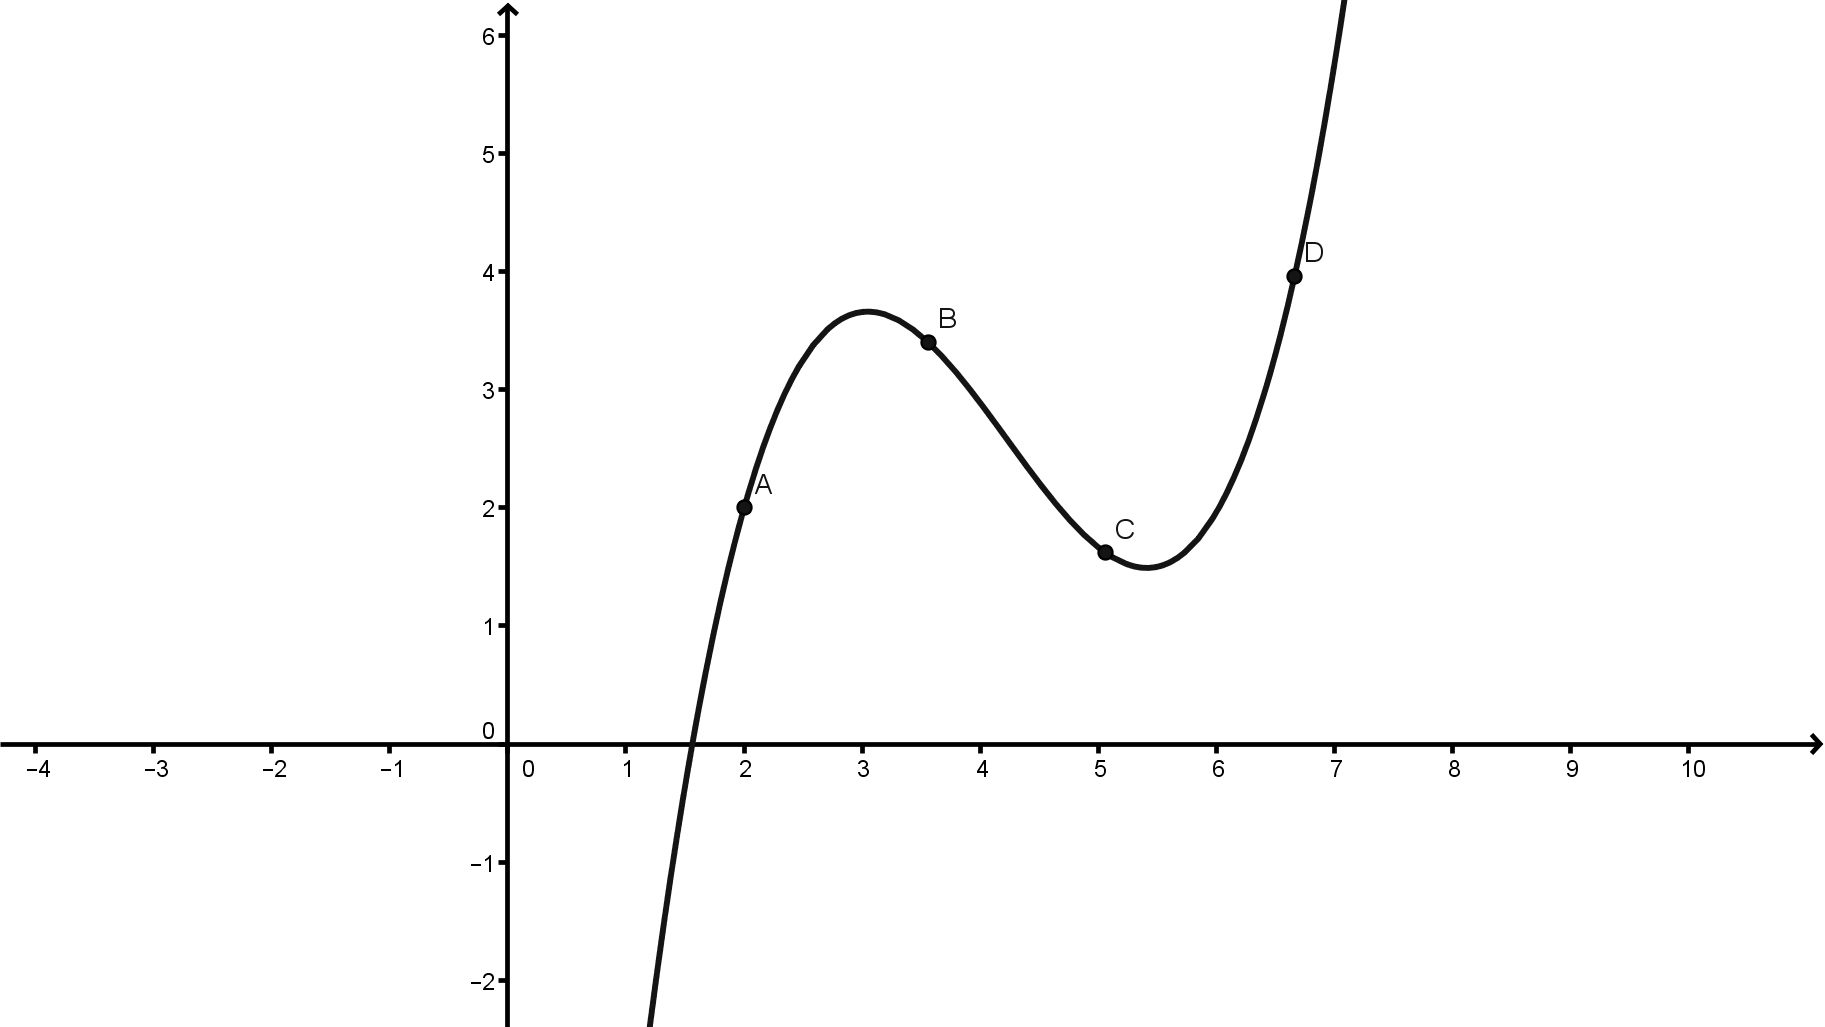
\includegraphics[width=12cm]{../fig/Cap10-Interpolacion02-bn.png}\\
(b) El polinomio de grado tres que pasa por esos cuatro puntos.
\end{bn}
\caption{Interpolación.}
\label{cap10:fig:Interpolacion01}
\end{center}
\end{figure}

Esta fórmula puede parecer muy impresionante, pero lo cierto es que tiene varios problemas. Un problema evidente es la complejidad de la propia fórmula. Si tenemos $50$ observaciones, lo cual no es demasiado, el polinomio de interpolación será de grado $51$ (un auténtico espanto, en general).

Pero es que, además, por si eso no fuera suficiente, hay un problema que, para lo que estamos tratando de hacer, es mucho peor. Para ayudarte a descubrirlo, en el Tutorial10 usaremos el ordenador para ayudarte a
%hemos preparado el fichero (con GeoGebra) \fichero{../datos/Cap10-ExperimentoInterpolacion.html}{Cap10-ExperimentoInterpolacion.html}, con el que puedes
%
comprobar que la {\em capacidad de predicción} de las fórmulas que proporciona la interpolación es, esencialmente, {\em nula}: si  añadimos un punto más, la curva que produce la fórmula cambia por completo, y los  valores que predice no tienen nada que ver con los anteriores. Ese comportamiento es, para lo que pretendemos hacer aquí, claramente indeseable. Querríamos una fórmula que fuese bastante estable al añadir o quitar un punto, porque eso nos permite intuir que tendrá una buena capacidad predictiva.

No queremos, no obstante, que pienses que la interpolación no sirve para nada. Es una herramienta extraordinariamente útil, {\em cuando se usa en el contexto adecuado}. Pero cuando se usa con datos experimentales, en el contexto que estamos discutiendo aquí, normalmente está fuera de lugar. Este problema tiene que ver con una conflicto habitual en Estadística, el problema del {\sf sobreajuste}\index{sobreajuste} (en inglés {\em overfitting}\index{overfitting}). Ese problema se refiere precisamente al hecho de que, a veces, al tratar de construir un modelo que explique los datos experimentales, los investigadores {\em se pasan de la raya}, y terminan con un modelo con escasa capacidad predictiva. Un modelo muy bueno para explicar lo que ya sabemos (los datos observados), pero que no nos ayuda a predecir. Para describir coloquialmente este problema, algunos estadísticos dicen que el sobreajuste consiste en confundir la {\em señal con el ruido}. Puedes leer una discusión reciente del problema en el libro titulado precisamente {\em The Signal and the Noise}, de Nate Silver (referencia \cite{silver2012signal}). Usar la interpolación aquí, para hacer que la fórmula explique todos los valores observados, sería un caso extremo de sobreajuste.

En los problemas como el del {\em Herrerillo}, que estamos usando de ejemplo, esta discusión es especialmente relevante. En un problema como ese estamos tratando de estudiar la relación entre dos variables, pero no podemos actuar como si no hubiera ningún otro factor que afectara a nuestras observaciones. En las medidas que hicieron los científicos no se reflejan otras variables que tal vez estén afectando al proceso (por ejemplo, no sabemos si hubo variaciones en la dieta durante el periodo de incubación, o cambios en el plumaje, o en la humedad del aire, etc.) La presencia de esas otras {\sf variables intrusas}\index{variables intrusas} o {\sf variables de confusión}\index{confusión, variables de}\index{variables de confusión} (en inglés, {\em confounding variables}\index{confounding variables}). Todas esas variables están presentes en nuestras medidas, muy especialmente en los estudios observacionales (como los estudios de campo, encuestas, etc.) y más controladas (pero aún así, siempre presentes) en los experimentos de laboratorio. El mayor desafío del Diseño Experimental es aislar, en la medida de lo posible, la relación que queremos estudiar del efecto de estas variables intrusas. Pero el hecho es que su presencia es inevitable, y se traduce en que, salvo en los casos más cercanos al ideal, los datos son {\em ruidosos}.

En la práctica, eso significa que, para avanzar, los científicos a menudo renuncian a encontrar esa fórmula ideal, y se conforman con una expresión que describa suficientemente bien los datos que tenemos, asumiendo que incluyen un cierto nivel de ruido, y que por lo tanto, son en gran medida aleatorios. Esas otras fórmulas ``ideales'', como la de la gravedad de Newton, no se obtienen de la observación, sino que se {\em deducen de la teoría}, usando modelos matemáticos de los mecanismos que causan el proceso que observamos. De nuevo, volvemos a ver el papel que la causalidad juega en este tema de la relación entre variables. En muchos aspectos de la ciencia y la técnica, esos mecanismos causales no son conocidos, y recurrimos a las fórmulas descriptivas, con el objetivo que ya hemos mencionado varias veces, de {\em predecir}.

¿Cómo podemos elegir una buena fórmula? Una que, a la vez, sea sencilla, estable para tener capacidad de predicción, y que represente bien al conjunto de puntos. Para obtener algo sencillo, conviene empezar con cosas sencillas. Eso es lo que vamos a hacer en la próxima sección.

\section{Recta de regresión, error cuadrático y correlación.}
\label{cap10:sec:RectaRegresionECCorrelacion}

Así que nos preguntamos ¿cuáles son las funciones más sencillas de todas?  En la Figura 5 que acompaña al artículo original, y que aquí reproducimos como Figura \ref{cap10:fig:Herrerillo} (pág. \pageref{cap10:fig:Herrerillo}), los investigadores reflejan, sobre un par de ejes de coordenadas, el diagrama de dispersión con las mediciones que hicieron de pares datos, con la temperatura en el eje $x$, y el consumo de  oxígeno en el eje $y$. Se muestran dos series de datos, correspondientes a dos situaciones posibles (incubando o no incubando). Ver el pie de la imagen para más detalles.

Y como puedes ver en esa figura, los investigadores han dibujado además dos rectas (una para cada serie de datos). Esas rectas, que llamaremos {\em rectas de regresión}, no se esfuerzan en {\em pasar por los datos individuales}, sino que tratan de representar de la mejor manera posible al conjunto o serie de datos. De nuevo, puedes pensar en esas rectas como un paso más en la dirección de hacer precisa la intuición que reflejaba la flecha de la Figura \ref{cap10:fig:Herrerillo02} (pág. \pageref{cap10:fig:Herrerillo02}). La recta, al fin y al cabo, es como la flecha, básicamente una forma de indicar la dirección o tendencia de nuestros datos. Pero la recta tiene una ecuación de la forma $y=f(x)$, así que nos va a permitir una descripción mucho más precisa, en cuanto comprendamos los detalles técnicos necesarios.

\begin{figure}[p]
\begin{center}
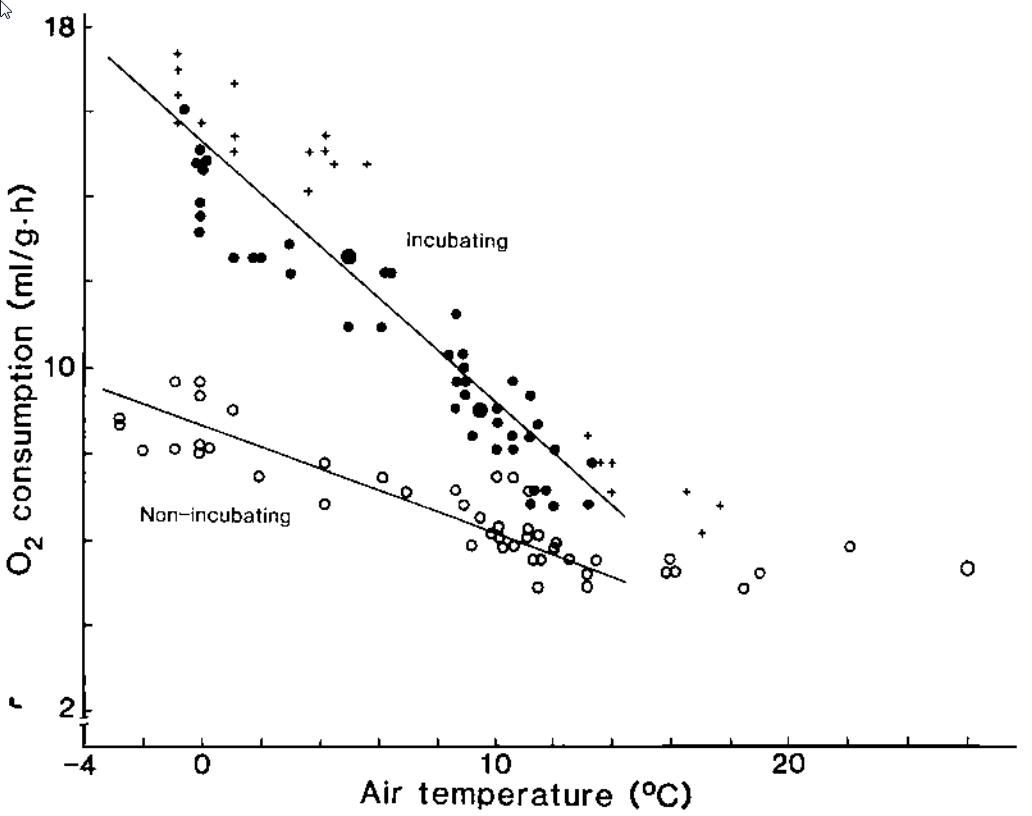
\includegraphics[width=13cm]{../fig/Cap10-Figura05HaftornReinertsenHerrerillos.png}
\caption[caption]{Reproducción de la Figura 5 del artículo \cite{haftorn1985effect} de S. Haftorn y R. E. Reinertsen, ``The effect of temperature and clutch size on the energetic cost of incubation in a free-living blue tit (parus caeruleus)", The Auk, pp. 470–478, 1985.. La figura aparece en la  pág. 473. El pie de la figura dice: {\em\small Relación entre la tasa de consumo de oxígeno de una hembra de {\em Herrerillo Común} cuando está en pie sobre los huevos, sin incubarlos (círculos abiertos), y cuando está incubando 13 huevos (círculos sólidos) [...]. Recta de regresión superior ($n=71$): $y=15.35-0.62x$. Recta de regresión inferior($n=41$): $y=8.45-0.22x$. Datos de 1983.}
\\\hspace{\textwidth}
Original en inglés: {\small\em The relationship between the female Blue Tit's oxygen-consumption rate and the air temperature, when standing over the eggs without incubating (open circles) and when incubating 13 eggs (solid circles). Crosses represent the oxygen-consumption rate on the day before hatching. Each record represents the stable value of oxygen-consumption rate at a stable air temperature. Large circles represent several equal records. Upper regression line ($n=71$): $y=15.35-0.62x$. Lower regression line ($n=41$): $y=8.45-0.22x$. Data from 1983.}
}
\label{cap10:fig:Herrerillo}
\end{center}
\end{figure}

¿Por qué una recta? Por su sencillez, desde luego. Está claro que las rectas no son siempre la mejor respuesta, pero para empezar son un buen punto de partida. Dejando de lado las constantes (que se pasan de sencillez) está claro que las rectas son las funciones con las gráficas, y las ecuaciones, más simples de todas. Una recta es una función de la forma:
\[y=b_0+b_1\cdot x\]
donde $b_0$ y $b_1$ son dos números, la {\sf ordenada en el origen}\index{ordenada en el origen} y la  {\sf pendiente}\index{pendiente de una recta} respectivamente. En el Tutorial10 usaremos el ordenador para explorar, de forma dinámica, el significado geométrico de estos valores.
%puedes recordar con ayuda del fichero GeoGebra  adjunto \fichero{../datos/Cap10-EcuacionRectaPendienteOrdenadaOrigen.html}{Cap10-EcuacionRectaPendienteOrdenadaOrigen.html}.
En particular veremos que cambiando los valores de $b_0$ y $b_1$ podemos obtener todas las rectas del plano (salvo las verticales, que no vamos a necesitar). Y entonces podemos hacer la siguiente pregunta clave: {\em de entre todas esas infinitas rectas, ¿cuál es la que mejor representa a nuestro conjunto de puntos?} Y más concretamente, {\em ¿cuáles son los valores de $b_0$ y $b_1$ que corresponden a la mejor recta posible?}

En el Tutorial10 usaremos el ordenador para afianzar nuestra intuición sobre ese concepto de  {\em la mejor recta posible}. En particular, dada una colección de puntos, podrás usar el ordenador para elegir la que a ti te parezca que es la mejor recta posible. Después podrás ver la respuesta que proporciona la Estadística, y ver si se parece a la tuya.
%
%Para ayudarte a intuir lo que queremos decir con esta idea de {\em la mejor recta posible} hemos preparado otro fichero GeoGebra, el fichero adjunto \fichero{../datos/Cap10-LaRectaDeRegresion.html}{Cap10-LaRectaDeRegresion.html}. Abre el fichero y mueve los puntos $M$ y $N$ para tratar de intuir cual es la mejor recta. Después, puedes ver la respuesta que proporciona la Estadística, y ver si has acertado.
%
Como adelanto de lo que podrás practicar en el Tutorial10, en la Figura \ref{cap10:fig:AjusteRectaPuntos} (pág. \pageref{cap10:fig:AjusteRectaPuntos}) puedes ver dos intentos de ajustar una recta a los datos, con bastante acierto en (a), y considerablemente peor  en (b).

\begin{figure}[htbp]
\begin{center}
\begin{enColor}
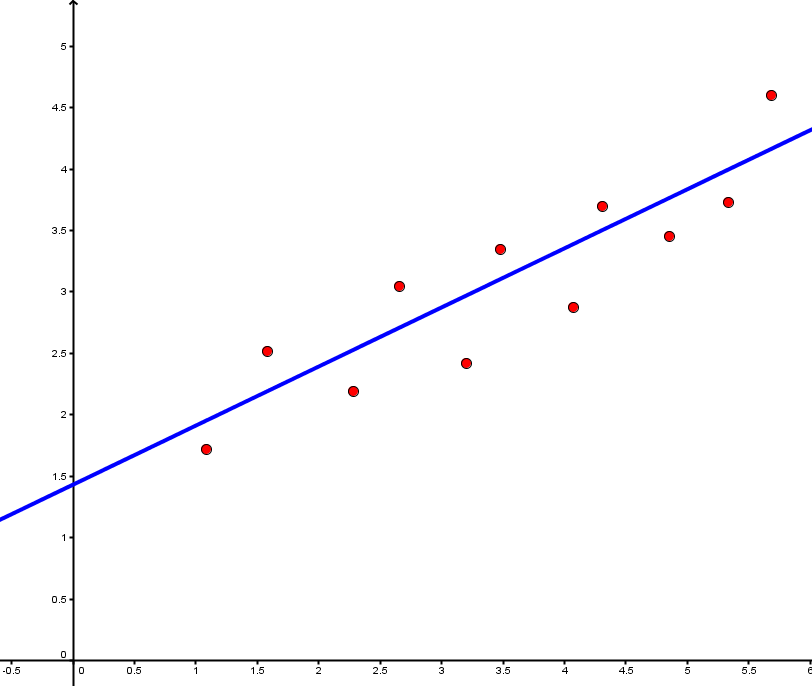
\includegraphics[width=10cm]{../fig/Cap10-RectaRegresionBuenIntento.png}\\
(a) Un buen intento de ajustar una recta a los datos.\\
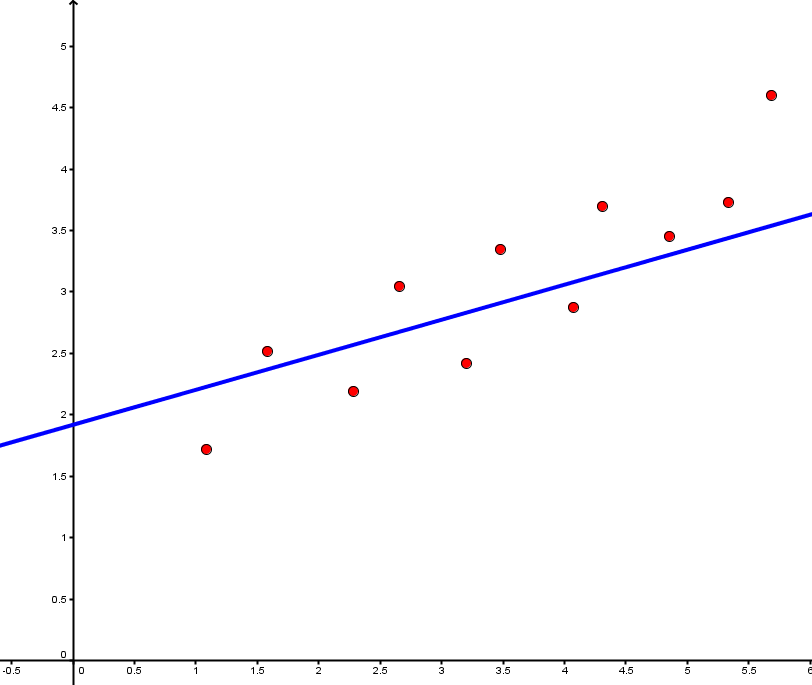
\includegraphics[width=10cm]{../fig/Cap10-RectaRegresionMalIntento.png}\\
(b) Un intento bastante peor.
\end{enColor}
\begin{bn}
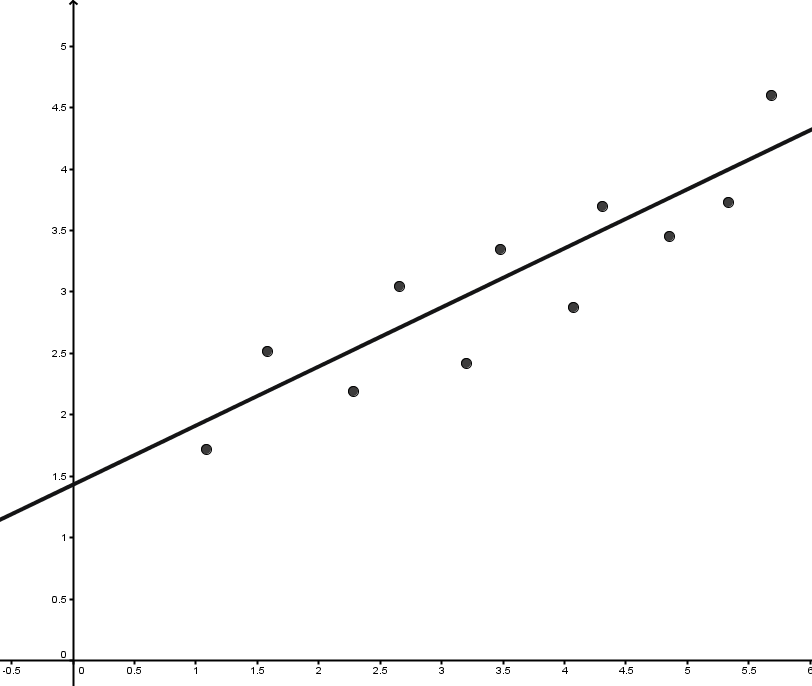
\includegraphics[width=10cm]{../fig/Cap10-RectaRegresionBuenIntento-bn.png}\\
(a) Un buen intento de ajustar una recta a los datos.\\
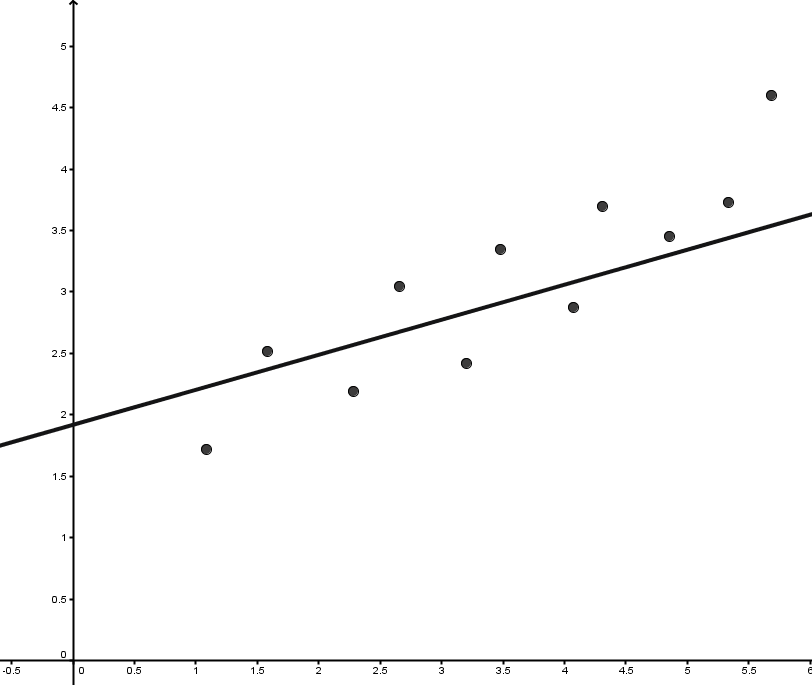
\includegraphics[width=10cm]{../fig/Cap10-RectaRegresionMalIntento-bn.png}\\
(b) Un intento bastante peor.
\end{bn}
\caption{Dos intentos, tratando de ajustar una recta a un mismo conjunto de puntos. Intuitivamente, la recta en (b) deja ``demasiados puntos por encima''.}
\label{cap10:fig:AjusteRectaPuntos}
\end{center}
\end{figure}

\subsection{¿Cómo elegir la mejor recta?}
\label{cap10:subsec:ComoElegirLaMejorRecta}

En el ejemplo de los herrerillos, vemos en el pie de la Figura \ref{cap10:fig:Herrerillo} que los investigadores proponen (para la serie ``no incubando'' de datos) esta recta:
\[y=8.45-0.22x.\]
Aquí $x$ es la temperatura del aire en grados centígrados, fácil de medir, como hemos dicho, mientras que $y$ es la tasa de consumo de oxígeno del ave (en $ml/(g\cdot h$)), que es desde luego mucho más difícil de medir. Esta fórmula nos permite, por ejemplo, predecir la tasa de consumo de oxígeno cuando $x=8^0$C, y ese es un valor que, por lo que se ve en la gráfica, seguramente no aparece en ninguno de los datos que los investigadores midieron directamente.

Hay varias preguntas que surgen inmediatamente, y a las que vamos a empezar a dar respuesta en esta sección:
\begin{itemize}
  \item ¿Cómo se han obtenido esos valores de $b_0$ y $b_1$? Esos valores tiene que garantizar que elegimos la mejor recta posible, en un sentido que intuimos (recuerda la Figura \ref{cap10:fig:AjusteRectaPuntos}), pero que debemos precisar.
  \item Una vez elegida esa recta, ¿cómo podemos usarla correctamente? Por, ejemplo, ¿podemos usarla para predecir el consumo de oxígeno a $30$ grados?
  \item ¿Cómo podemos medir la calidad de la recta que hemos obtenido? Es decir, puede sucede que tengamos la mejor recta, y que aún así la mejor recta sea una muy mala representación de los datos. Daremos ejemplos y más detalles pronto.
\end{itemize}

Empezando por la primera pregunta. Para entender la respuesta, tenemos que reflexionar un poco sobre el uso que pensamos darle a la recta que vamos a obtener. El objetivo, repetimos, es que, una vez que tengamos la ecuación
\[y=b_0+b_1\cdot x,\]
cada vez que obtengamos un valor de la variable $x$ podamos utilizar esta ecuación para
predecir el valor de $y$ sin necesidad de medirlo directamente.

Con esta reflexión podemos avanzar un poco más en la determinación de la recta. Lo que
esperamos de esa recta es que sea buena prediciendo los valores de $y$. Nosotros la
obtenemos a partir de una muestra formada por este conjunto de puntos:
\[(x_1,y_1),\, (x_2,y_2),\, (x_3,y_3),\, \ldots,\, (x_n,y_n),\]
Pero si consideramos {\em por separado} los valores de la coordenada $x$, que son:
\[x_1, x_2,\ldots, x_n,\]
y los sustituimos en la ecuación de la recta, obtendremos una colección de {\sf valores
predichos (o ajustados)}\index{valores predichos}\index{valores ajustados}\index{predichos, valores}\index{ajustados, valores} (en inglés, {\em fitted values}\index{fitted values}):
\[\hat y_1, \hat y_2, \ldots, \hat y_n,\]
donde, por supuesto,
\begin{equation}
\label{cap10:ecu:FittedValues}
    \phantom{123456123456123456}\hat y_i=b_0+b_1\cdot x_i,\quad\mbox{ para }i=1,\ldots,n.
\end{equation}
Y ahora podemos precisar lo que queremos: la recta será la mejor posible si estos valores
predichos se parecen lo más posible, en promedio (que para eso estamos haciendo Estadística), a los valores iniciales de la coordenada $y$.

Esta forma de plantear el problema nos devuelve a un terreno conocido: para medir cómo se parecen esos dos conjuntos de valores consideramos las diferencias o {\sf residuos}\index{residuo (en la regresión lineal)} (en inglés, {\em residuals}\index{residuals (in linear regresión)}):
\begin{equation}\label{cap10:ecu:ResiduosRegresionLineal}
e_1=y_1-\hat y_1,\, e_2=y_2-\hat y_2,\, \ldots, e_n=y_n-\hat y_n,
\end{equation}
Y ¿qué hacemos, las promediamos? No, a estas alturas ya sabemos que promediar diferencias,
sin más, no es una buena idea, {\em porque las diferencias positivas muy grandes pueden
compensarse con diferencias negativas muy grandes,  y engañarnos}. Para conseguir una
información fiable, tenemos que pagar el peaje de elevar al cuadrado las diferencias,
y entonces promediaremos. La definición del objeto que usaremos como base para medir la calidad de la recta es esta:
    \begin{center}
    \fcolorbox{black}{Gris025}{
    \begin{minipage}{12.5cm}
        \begin{center}
        %%%%%%%%%%%%%%%%%%%%%%%%%%%%%%%%%%%%%%%
        {\bf \sf Error cuadrático.}
        \index{error cuadrático (en la regresión lineal)}
        \end{center}
       %%%%%%%%%%%%%%%%%%%%%%%%%%%%%%%%%%%%%%%
         Dado el conjunto de puntos
         \[(x_1,y_1),(x_2,y_2),(x_3,y_3),\ldots,(x_n,y_n),\]
         si consideramos los valores predichos:
          \[\hat y_1,\hat y_2,\ldots,\hat y_n,\]
         siendo,
        \[\hat y_i=b_0+b_1\cdot x_i,\quad\mbox{ para }i=1,\ldots,n,\]
        entonces el {\sf error cuadrático} (en inglés {\em sum of squared errors}) de la recta $y=b_0+b_1\cdot x$ es:
        \begin{equation}\label{cap10:ecu:ErrorCuadratico}
        \mbox{EC}(y=b_0+b_1\cdot x)=\sum_{i=1}^n(y_i-\hat y_i)^2=
        \sum_{i=1}^n(y_i-b_0-b_1\cdot x_i)^2.
        \end{equation}
        El error cuadrático medio ECM\index{error cuadrático medio} es simplemente el promedio muestral (decimos muestral porque usamos $n-1$; luego quedará claro el motivo):
        \begin{equation}\label{cap10:ecu:ECM}ECM=\dfrac{EC}{n-1}.\end{equation}
       %%%%%%%%%%%%%%%%%%%%%%%%%%%%%%%%%%%%%%%
    \end{minipage}}
    \end{center}
Hemos llegado hasta el error cuadrático pensando en minimizar la diferencia entre los valores observados y los que predice la recta. Pero es bueno acompañar esta noción de una cierta intuición geométrica. Para cada punto observado $(x_i,y_i)$, podemos considerar el correspondiente punto sobre la recta, $(x_i,\hat y_i)$, y construir un cuadrado (porque el error es cuadrático) de lado $(y_i-\hat y_i)$, como se muestra en la Figura \ref{cap10:fig:InterpretacionErrorCuadratico}. El error cuadrático depende de los puntos $(x_i,y_i)$ y, por supuesto, de la recta
que se utilice. Para cada recta que elegimos, el error cuadrático toma un valor distinto, que puede ser muy grande si la recta se aleja de los puntos. En el Tutorial10 usaremos el ordenador para explorar, de forma dinámica, como cambia el error cuadrático cuando cambiamos la recta.
%fichero GeoGebra adjunto, llamado \fichero{../datos/Cap10-InterpretacionErrorCuadratico.html}{Cap10-InterpretacionErrorCuadratico.html}, puedes experimentar con esta idea de error cuadrático, moviendo la recta y viendo como cambia el valor de ese error.

\begin{figure}[htbp]
\begin{center}
\begin{enColor}
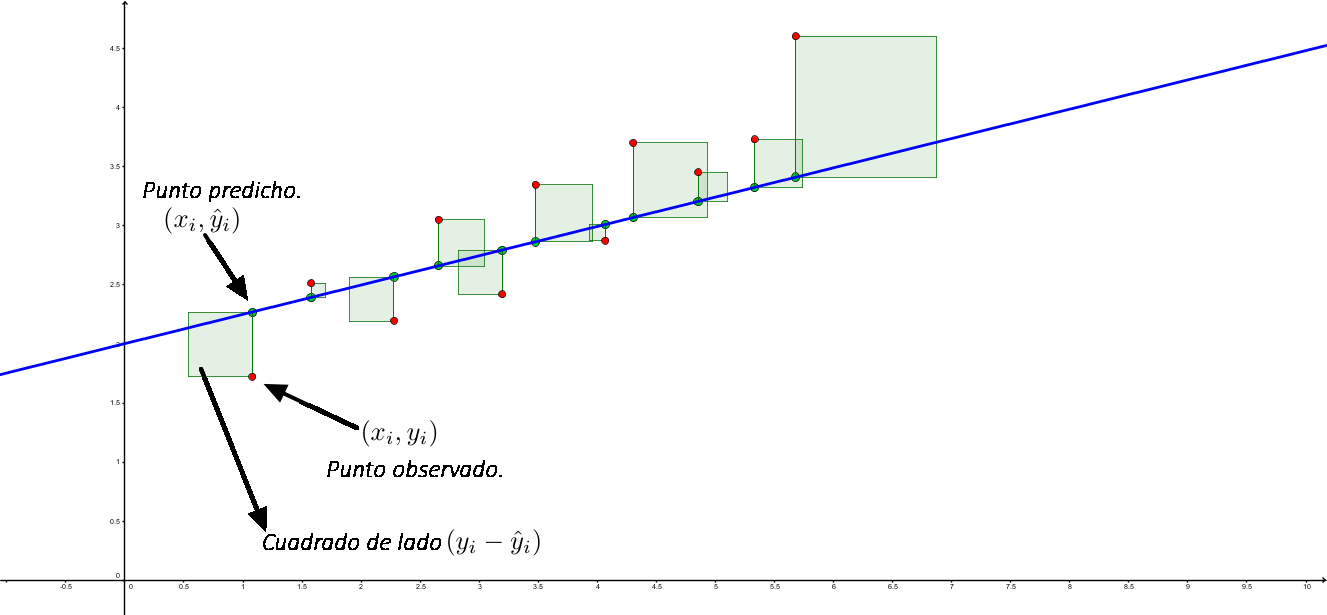
\includegraphics[width=14cm]{../fig/Cap10-InterpretacionErrorCuadratico.png}
\end{enColor}
\begin{bn}
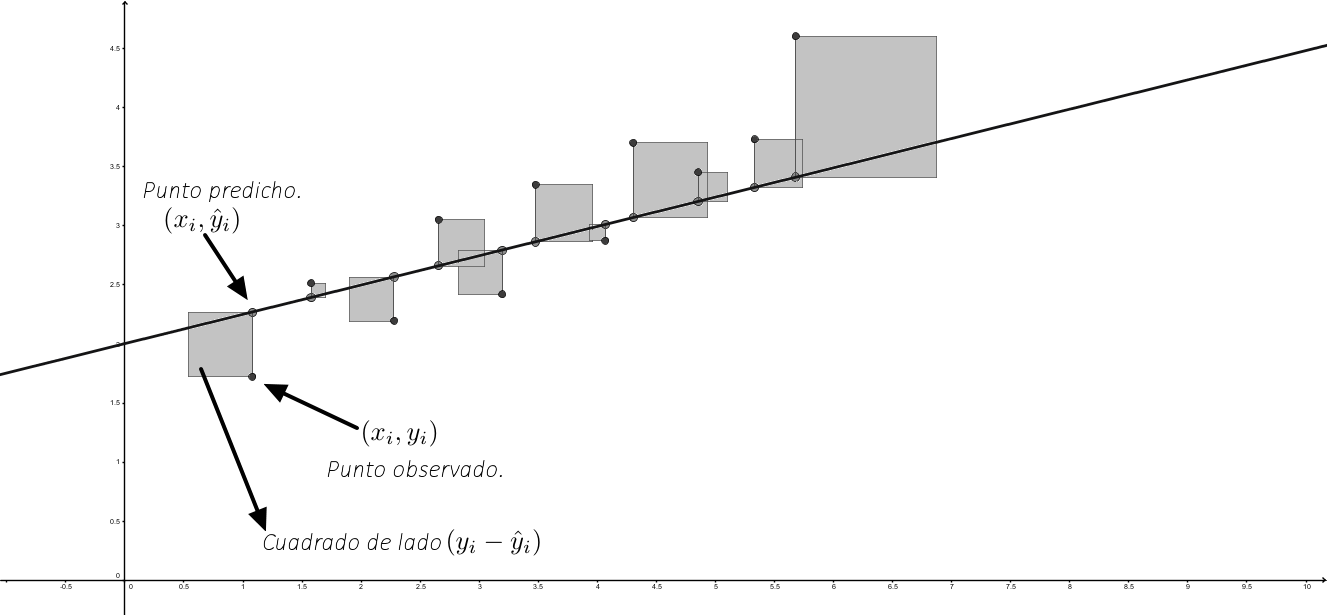
\includegraphics[width=14cm]{../fig/Cap10-InterpretacionErrorCuadratico-bn.png}
\end{bn}
\caption{Interpretación geométrica del error cuadrático. La recta es una recta cualquiera.}
\label{cap10:fig:InterpretacionErrorCuadratico}
\end{center}
\end{figure}
Una vez definido el error cuadrático,  la búsqueda de la mejor recta se puede formular de una manera mucho más precisa:

\begin{center}
\fcolorbox{black}{Gris025}{
\begin{minipage}{12.5cm}
%%%%%%%%%%%%%%%%%%%%%%%%%%%%%%%%%%%%%%%
¿Cuáles son los valores $b_0$ y $b_1$ para los que  la recta
    \[y=b_0+b_1\cdot x\]
produce el valor mínimo posible del error cuadrático?
%%%%%%%%%%%%%%%%%%%%%%%%%%%%%%%%%%%%%%%
\end{minipage}
}
\end{center}
Es decir, ¿cómo hay que colocar la recta, usando $b_0$ y $b_1$, para que la suma de las áreas de los cuadrados de la Figura \ref{cap10:fig:InterpretacionErrorCuadratico} sea mínima?

Y, ya que estamos, vamos a plantearnos otra pregunta, relacionada con esta. Más adelante será útil haber pensado en esto: el error cuadrático siempre es positivo o $0$. ¿En qué caso especial se obtiene $EC=0$? Si lo piensas un poco te darás cuenta de que esto sólo puede suceder si, para empezar, los puntos
\[(x_1,y_1),\ldots,(x_n,y_n)\]
ya estaban, para empezar, alineados sobre una recta, como se muestra en la Figura \ref{cap10:fig:ErrorCuadraticoIgual0}. En ese caso, desde luego, la mejor recta posible para representar a esos puntos será esa misma recta sobre la que se encuentran. Además, en ese caso, se cumplirá $y_i=\hat y_i$, naturalmente.

\begin{figure}[htbp]
\begin{center}
\begin{enColor}
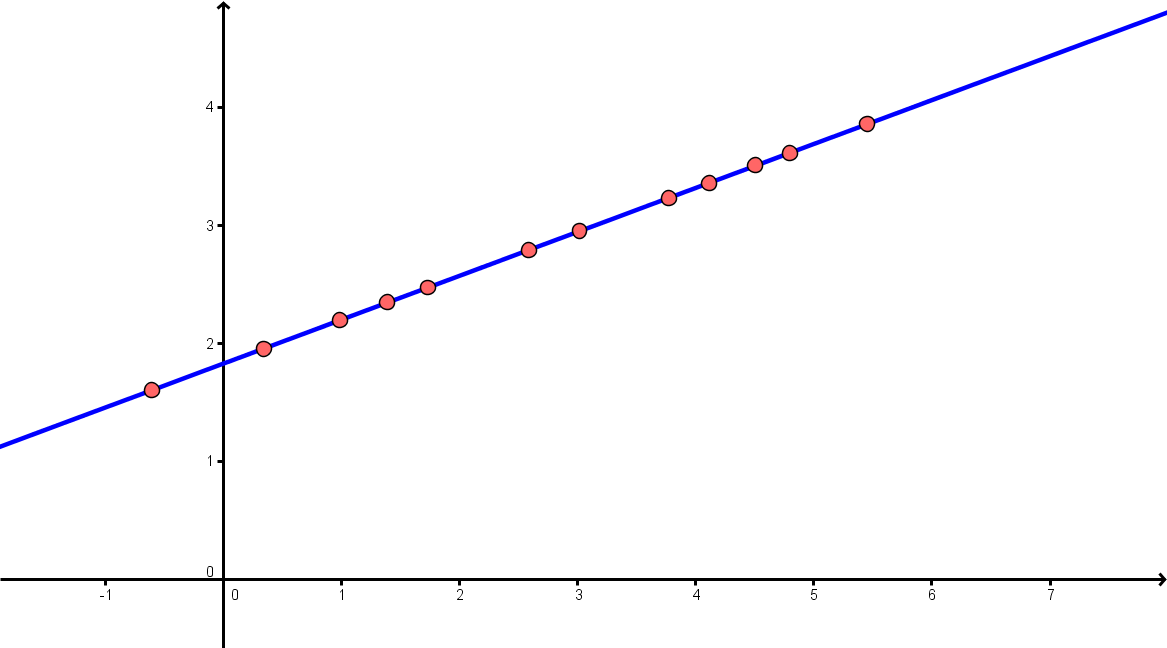
\includegraphics[width=11cm]{../fig/Cap10-ErrorCuadraticoIgual0.png}
\end{enColor}
\begin{bn}
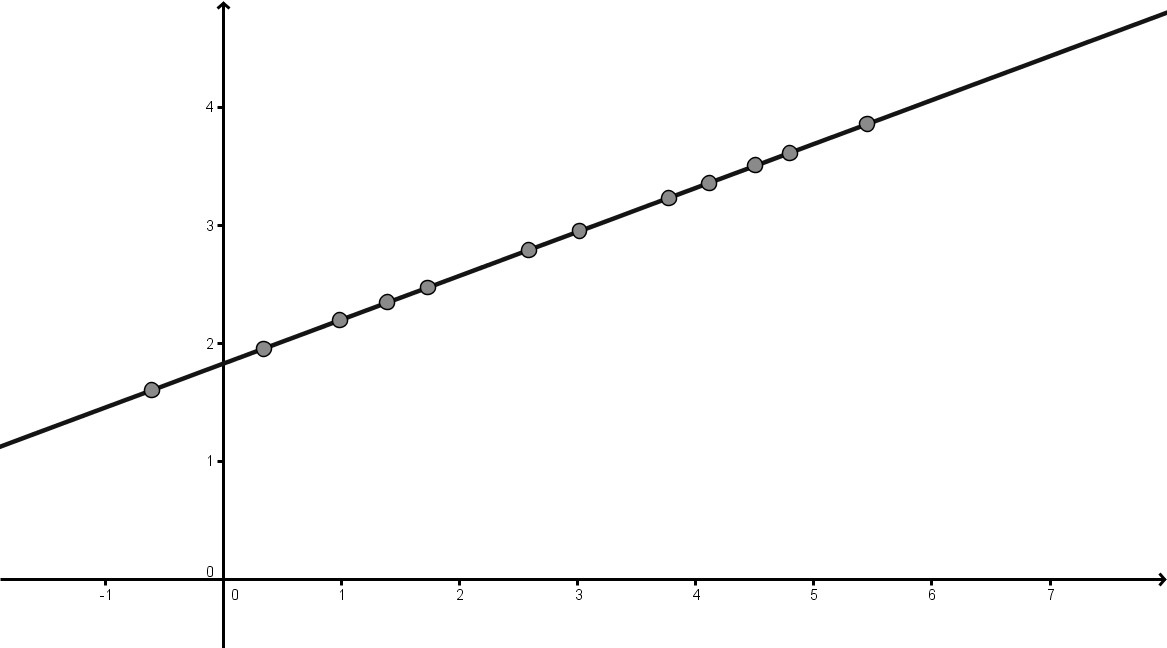
\includegraphics[width=11cm]{../fig/Cap10-ErrorCuadraticoIgual0-bn.png}
\end{bn}
\caption{El único caso en el que $EC=0$ es el de los puntos situados en una recta.}
\label{cap10:fig:ErrorCuadraticoIgual0}
\end{center}
\end{figure}

Volvamos a la búsqueda de la mejor recta posible, en el caso general de puntos no alineados. Una vez fijados esos puntos $(x_i,y_i)$, el error cuadrático depende sólo de $b_0$ y de $b_1$. Tenemos una función
\[EC(b_0,b_1) = \sum_{i=1}^n(y_i-b_0-b_1\cdot x_i)^2.\]
Así que este es un problema de máximos y mínimos, como los que se estudian en Cálculo Diferencial. Posiblemente el lector haya aprendido que para hallar los máximos de una función hay que calcular su derivada e igualarla a $0$. La situación aquí es parecida, pero al tratarse de una función de dos variables, $b_0$ y $b_1$, hay que calcular las derivadas parciales e igualarlas a $0$:
\begin{equation}
\label{cap10:ecu:SistemaDerivadasParcialesMinimosCuadrados}
\begin{cases}
\dfrac{\partial EC(b_0,b_1)}{\partial b_0}=0\\[3mm]
\dfrac{\partial EC(b_0,b_1)}{\partial b_1}=0
\end{cases}
\end{equation}
La solución de este sistema de dos ecuaciones para las variables $b_0$ y $b_1$ (las coordenadas $(x_i, y_i)$ se consideran constantes dadas)  nos conduce a la recta que andamos buscando.  Y,
conociendo las herramientas necesarias, es fácil de resolver. No nos vamos a entretener en esos detalles técnicos, que el lector puede encontrar, por ejemplo, en la referencia \cite{garcia2009estadistica} (Sección 17.2, pág. 186), o en \cite{horra2003estadistica} (Capítulo 2, Sección 3, pág. 14).


Para entender mejor la expresión de la recta que se obtiene, al resolver ese sistema, es necesario introducir primero un poco de notación. Si pensamos {\em por separado} en los valores de la coordenada
$x$,
\[x_1, x_2,\ldots, x_n,\]
y en los valores iniciales de la coordenada $y$:
\[y_1, y_2,\ldots, y_n,\]
podemos definir sus medias y cuasivarianzas:
\[\bar x=\dfrac{\displaystyle\sum_{i=1}^{n}x_i}{n},\qquad s^2(x)=\dfrac{\displaystyle\sum_{i=1}^{n}(x_i-\bar x)^2}{n-1}\]
\[\bar y=\dfrac{\displaystyle\sum_{i=1}^{n}y_i}{n},\qquad s^2(y)=\dfrac{\displaystyle\sum_{i=1}^{n}(y_i-\bar y)^2}{n-1}\]
Vamos a utilizar estos valores para escribir la ecuación de la recta. El primer paso consiste en señalar que, con ellos, podemos construir un punto interesante: el que tiene por coordenadas $(\bar x,\bar y)$, las medias por separado. Si $\bar x$ es un buen representante de las coordenadas $x$, y $\bar y$ es un buen representante de las coordenadas $\bar y$, ¿será verdad que la mejor recta posible tiene que pasar por ese punto $(\bar x,\bar y)$? La respuesta es afirmativa, y nos permite escribir la recta que buscamos de una forma muy conveniente para interpretarla.
    \begin{center}
    \fcolorbox{black}{Gris025}{
    \begin{minipage}{12.5cm}
        \begin{center}
        %%%%%%%%%%%%%%%%%%%%%%%%%%%%%%%%%%%%%%%
        {\bf Recta de regresión (o de mínimos cuadrados). Covarianza.}
        \index{recta de regresión}
        \index{covarianza}
        \index{recta de mínimos cuadrados}
        \end{center}
       %%%%%%%%%%%%%%%%%%%%%%%%%%%%%%%%%%%%%%%
        Dado el conjunto de puntos $(x_1,y_1),(x_2,y_2),(x_3,y_3),\ldots,(x_n,y_n)$,
        la {\sf recta de regresión o de mínimos cuadrados} (en inglés, {\em regression line}\index{regression line} o también {\em line of best fit}\index{line of best fit}\index{best fit, line of}) es la recta que minimiza el error cuadrático EC. Esa recta puede escribirse en la forma:
        \begin{equation}\label{cap10:ecu:RectaRegresionFormaPuntoPendiente}
        (y-\bar y)=
        \dfrac{\colorbox{lightgrey}{$\Cov(x,y)$}}
        {s^2(x)}\cdot (x-\bar x),
        \end{equation}
        siendo
        \begin{equation}\label{cap10:ecu:Covarianza}
        \Cov(x,y)=\dfrac{\displaystyle\sum_{i=1}^{n}(x_i-\bar x)(y_i-\bar y)}{n-1}
        \end{equation}
        una nueva cantidad, que llamaremos la {\sf covarianza muestral}\index{covarianza muestral}
        (en inglés, {\em covariance}\index{covariance}) de $(x_1,y_1),\ldots,(x_n,y_n)$. Si la recta es $y=b_0+b_1\cdot x$, entonces:
        \begin{equation}\label{cap10:ecu:RectaRegresionPendienteOrdenadaOrigen}
        b_1=
        \dfrac{\Cov(x,y)}{s^2(x)},
        \qquad b_0= \bar y -
        \dfrac{\Cov(x,y)}{s^2(x)}\cdot\bar x.
        \end{equation}
       %%%%%%%%%%%%%%%%%%%%%%%%%%%%%%%%%%%%%%%
    \end{minipage}
    }
    \end{center}
Otra notación frecuente para la covarianza es $s^2_{x,y}$. El método que hemos utilizado para determinar la recta se conoce como {\sf método de mínimos cuadrados}\index{método de mínimos cuadrados}\index{mínimos cuadrados, método} (en inglés, {\em ordinary least squares}\index{ordinary least squares}\index{least squares}, a menudo abreviado {\sf OLS}\index{OLS, ordinary least squares}).
%Daremos algunos detalles sobre otros posibles métodos en el Apéndice \ref{apendice:MasAlla} (pág. \pageref{apendice:MasAlla}).

\noindent Fíjate, en particular, en que obtenemos esta expresión para el valor $\hat y_i$ que predice la recta en $x_i$:
\begin{equation}\label{cap10:ecu:ValorPrediceRectaRegresion}
\hat y_i=
\bar y + \dfrac{\Cov(x,y)}{s^2(x)}\cdot (x_i-\bar x) =
\bar y + b_1\cdot (x_i-\bar x).
\end{equation}

\noindent{\bf Una advertencia:} dependiendo del libro que uses, puedes encontrar la covarianza definida con $n$ en el denominador. Nosotros usaremos la Definición \ref{cap10:ecu:Covarianza}, con $n-1$, que coincide con lo que hace el software que usamos.

Y otra observación: el hecho de que la recta de regresión pase por el punto $(\bar x, \bar y)$  equivale a
decir que los residuos $e_i=y_i-\hat y_i$, {\em calculados para esa recta}, suman cero:
\begin{equation}
\label{cap10:ecu:SumaResiduosCeroRectaRegresion}
\sum_{i=1}^n e_i=\sum_{i=1}^n (y_i-\hat y_i)=0 \mbox{\em , para la recta de regresión.}
\end{equation}

\noindent Antes de seguir adelante, veamos un ejemplo.
\begin{ejemplo}\label{cap10:ejem:Regresion01}
Supongamos que tenemos estos $n=10$ puntos $(x_i,y_i)$:
\[(12.1,-3.3),(23.9,-8.9),(19.8,-6.9),(19.3,-6.4),(7.05,-0.67),(18.4,-6.2),\]
\[(22.9,-8.6),(20.2,-7.2),(23.4,-8.8),(20.7,-7.3)\]
Otra forma típica de darnos los datos es mediante una tabla, como la Tabla \ref{cap10:tabla:EjemploRegresion01}.
\begin{table}[ht]
\centering
\begin{tabular}{rrrrrrrrrrr}
  \hline
 & 1 & 2 & 3 & 4 & 5 & 6 & 7 & 8 & 9 & 10 \\
  \hline
$x$ & 12.1 & 23.9 & 19.80 & 19.3 & 7.05 & 18.4 & 22.90 & 20.20 & 23.4 & 20.7 \\
$y$ & -3.3 & -8.9 & -6.90 & -6.40 & -0.67 & -6.2 & -8.6 & -7.2 & -8.8 & -7.3 \\
   \hline
\end{tabular}
\caption{Datos del Ejemplo \ref{cap10:ejem:Regresion01}.}
\label{cap10:tabla:EjemploRegresion01}
\end{table}
En cualquier caso, a partir de estos datos calculamos (en el Tutorial10 aprenderemos a hacer estos cálculos con el ordenador):
\[
\bar x \approx 18.78
,\quad
s^2(x)\approx 28.21
\]
\[
\bar y \approx -6.427
,\quad
s^2(y)\approx 6.781
\]
Además:
\[\Cov(x,y)\approx -13.81\]
Por lo tanto, la pendiente de la recta es:
\[b_1=\dfrac{\Cov(x,y)}{\operatorname{Var}_n}(x)\approx -0.4896,\]
y a partir de $b_1$, usando la Ecuación \ref{cap10:ecu:RectaRegresionPendienteOrdenadaOrigen}, podemos calcular la ordenada en el origen:
\[b_0 \approx 2.766 \]
De modo que la recta de regresión buscada es, aproximadamente:
\[y = 2.766-0.4896\cdot x.\]
La Figura \ref{cap10:fig:EjemploRegresion01} muestra los puntos $(x,y)$ (círculos) junto con la recta de regresión que hemos obtenido.
\begin{figure}[htbp]
\begin{center}
\begin{enColor}
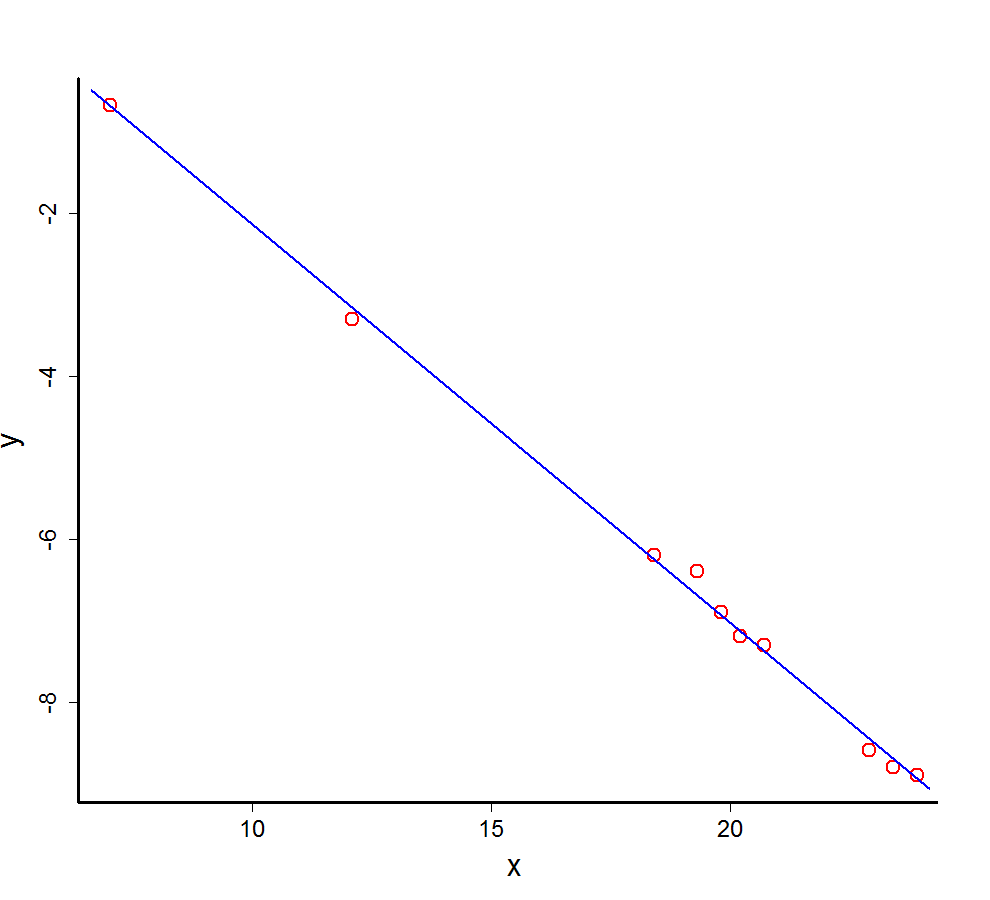
\includegraphics[width=9cm]{../fig/Cap10-EjemploRegresion01.png}
\end{enColor}
\begin{bn}
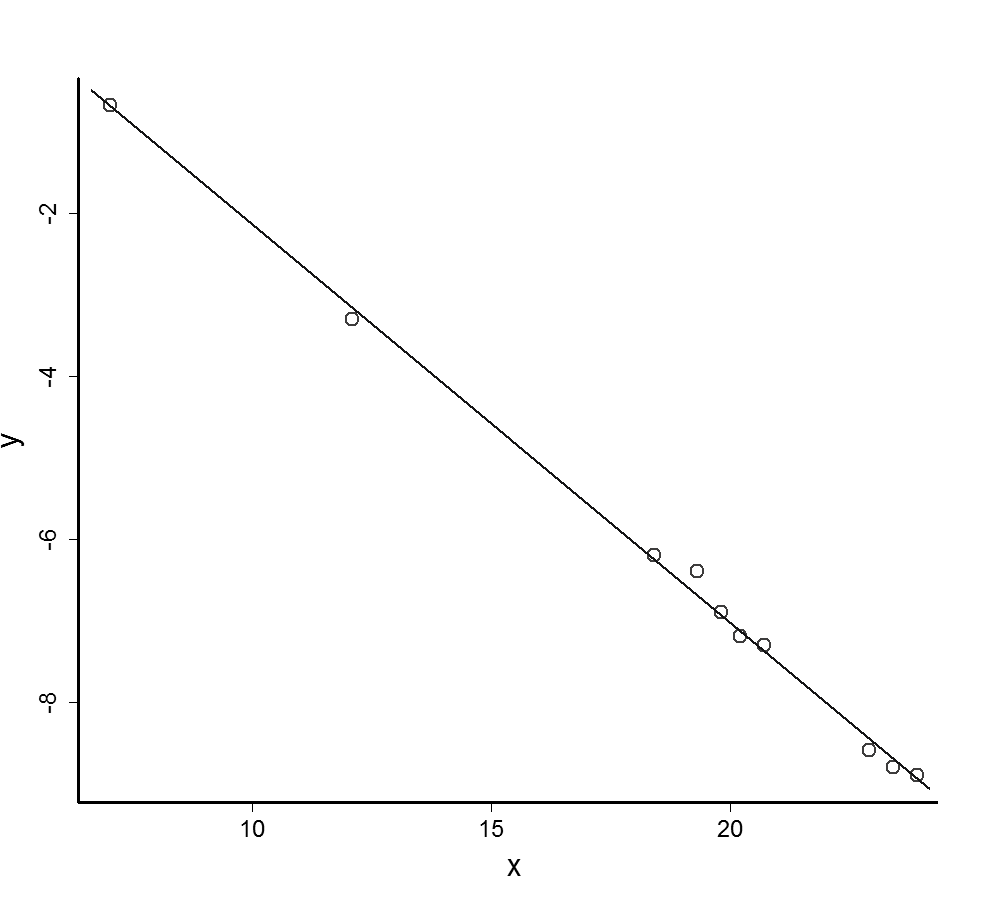
\includegraphics[width=9cm]{../fig/Cap10-EjemploRegresion01-bn.png}
\end{bn}
\caption{Puntos y recta de regresión del Ejemplo \ref{cap10:ejem:Regresion01}.}
\label{cap10:fig:EjemploRegresion01}
\end{center}
\end{figure}


\qed
\end{ejemplo}

\subsubsection{Reflexiones sobre el uso de rectas de regresión}
\label{cap10:subsubsec:ReflexionUsoRectaRegresion}

Recuerda que tenemos pendientes las dos últimas preguntas que hacíamos al comienzo de la Sección \ref{cap10:subsec:ComoElegirLaMejorRecta} (pág. \pageref{cap10:subsec:ComoElegirLaMejorRecta}). Antes de seguir adelante, y empezar a plantearnos la respuesta a esas preguntas, queremos dedicar un momento a pensar, en general, sobre la propia idea de usar rectas.

¿Por qué usamos rectas? Ya hemos dicho que la principal razón es porque son sencillas. Pero hay otras razones importantes. Vamos a ver algunas de ellas:

Para empezar, hay muchas otras situaciones en las que podemos hacer un cambio de variable, y resolver el problema en las nuevas variables usando una recta. Por ejemplo, si tenemos una función de la forma:
        \[y=4\cdot e^{3x+2}\]
y pasamos el $4$ al miembro izquierdo y tomamos logaritmos, se convierte en:
        \[\ln\left(\dfrac{y}{4}\right)=3x+2\]
Y si ahora hacemos el cambio de variables \[u=\ln\frac{y}{4},\] obtenemos
        \[u=3x+2\]
que es una recta en las nuevas variables $x,u$.  Hay muchas funciones (pero no todas)
que se pueden convertir en rectas mediante trucos de cambio de variable similares a este.

Hay otra propiedad de las rectas que las hace especialmente importantes, y que está en la base de la parte de las Matemáticas que llamamos Cálculo Diferencial. En el Tutorial10 tendremos ocasión de usar el ordenador para explorar estas ideas con más detalle. Aquí hemos incluido un resumen gráfico en la Figura \ref{cap10:fig:RectaComoAproximacionLocal}, para ilustrar de qué se trata. La idea, resumida mucho, es esta: tomamos una función cualquiera, que sea ``normal'' (que no haga cosas demasiado raras, quiebros, cambios bruscos de dirección, etc.). Nos fijamos en un punto cualquier de la gráfica de la función, y hacemos zoom acercándonos cada vez más a ese punto, como si lo observáramos al microscopio, cada vez con más aumentos. Entonces lo que veremos se parecerá cada vez más a una recta, que es la {\sf recta tangente}\index{recta tangente a una función}  a la función en el punto en el que hacemos zoom. En la Figura \ref{cap10:fig:RectaTangenteParabola}
hemos tratado de ilustrar esta idea, que es una de las más útiles de todas las Matemáticas.
\begin{figure}[htb]
\begin{center}
\begin{enColor}
\begin{tabular}{cc}
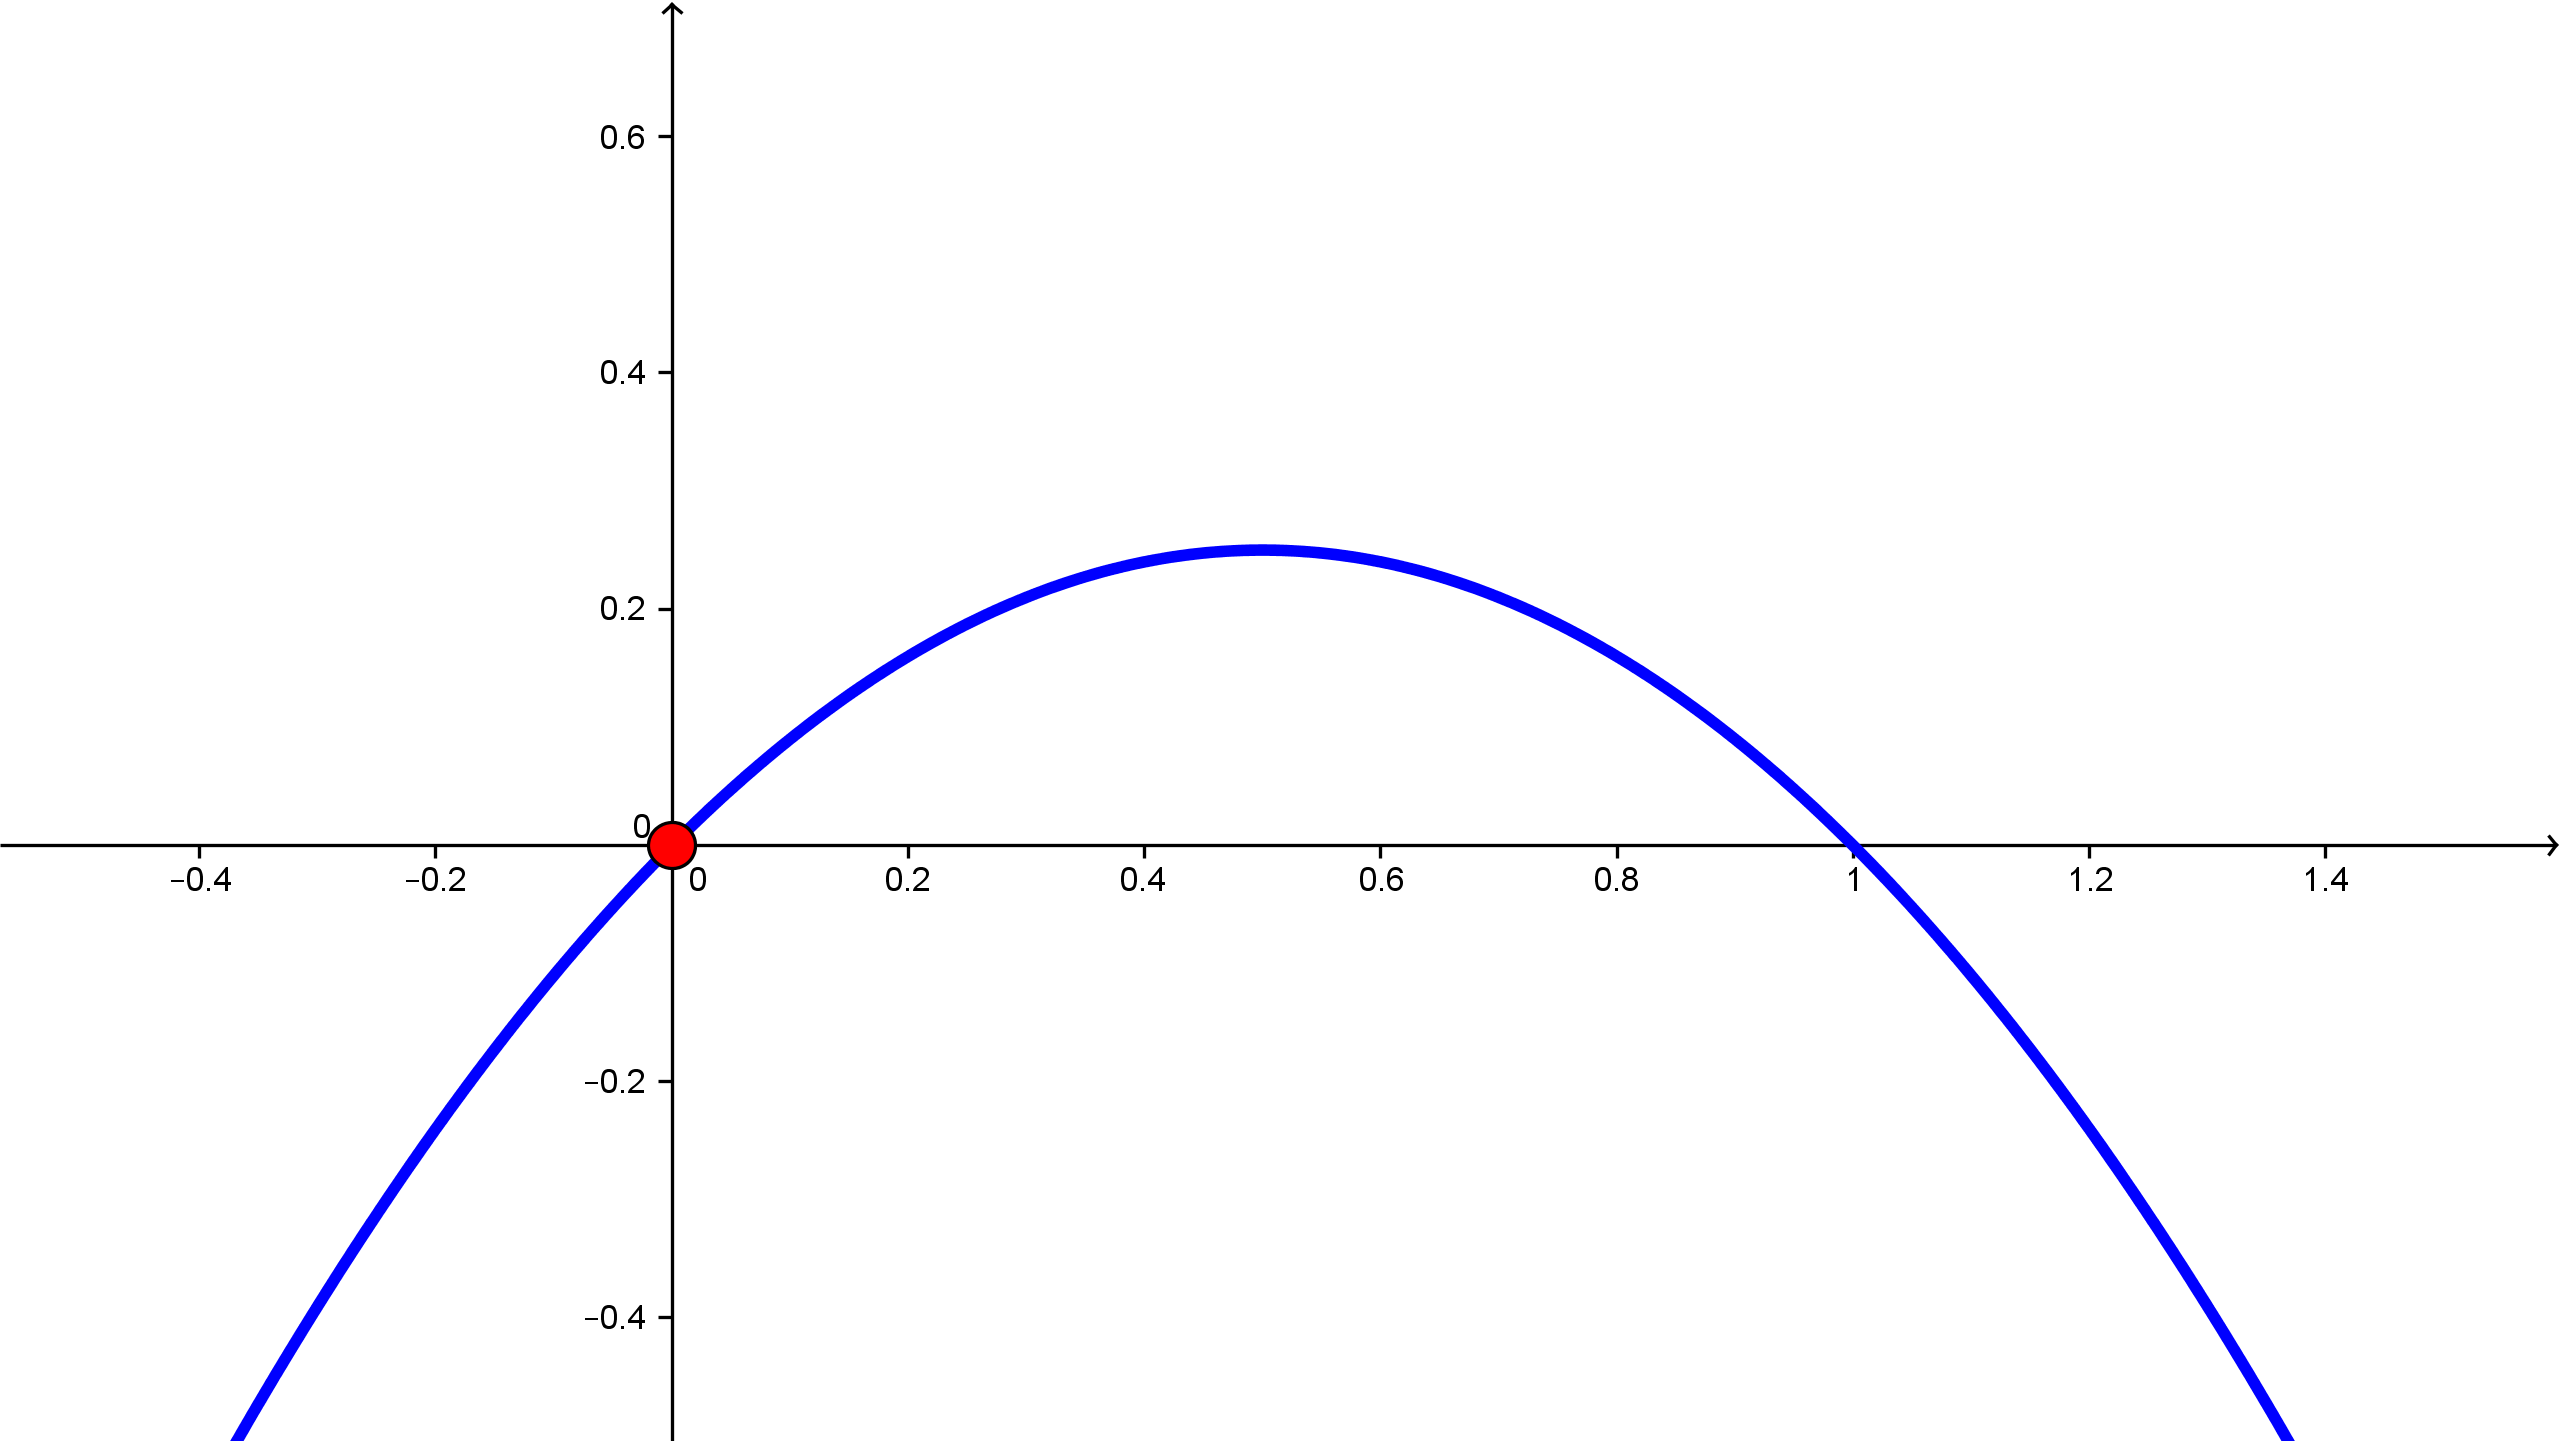
\includegraphics[width=6.5cm]{../fig/Cap10-ZoomEnParabola01.png}&
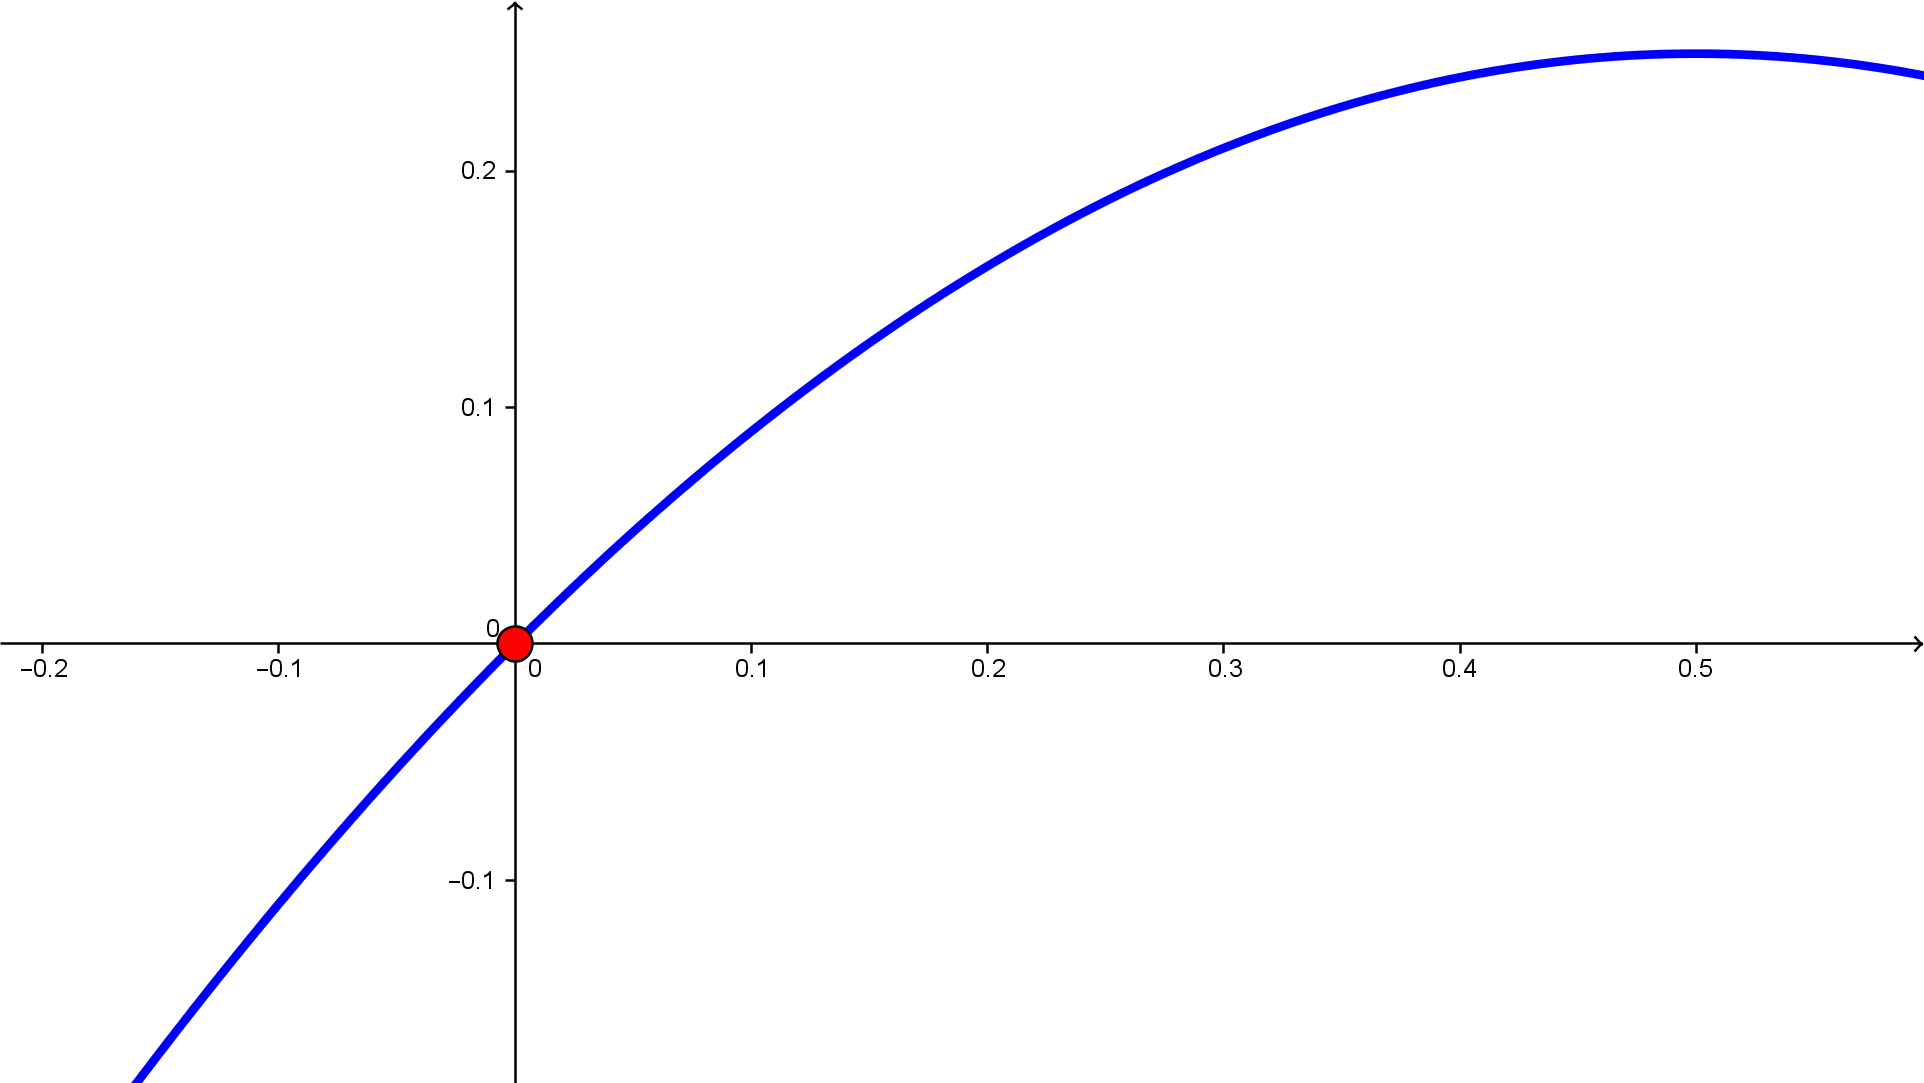
\includegraphics[width=6.5cm]{../fig/Cap10-ZoomEnParabola02.png}\\
(a)&(b)\\
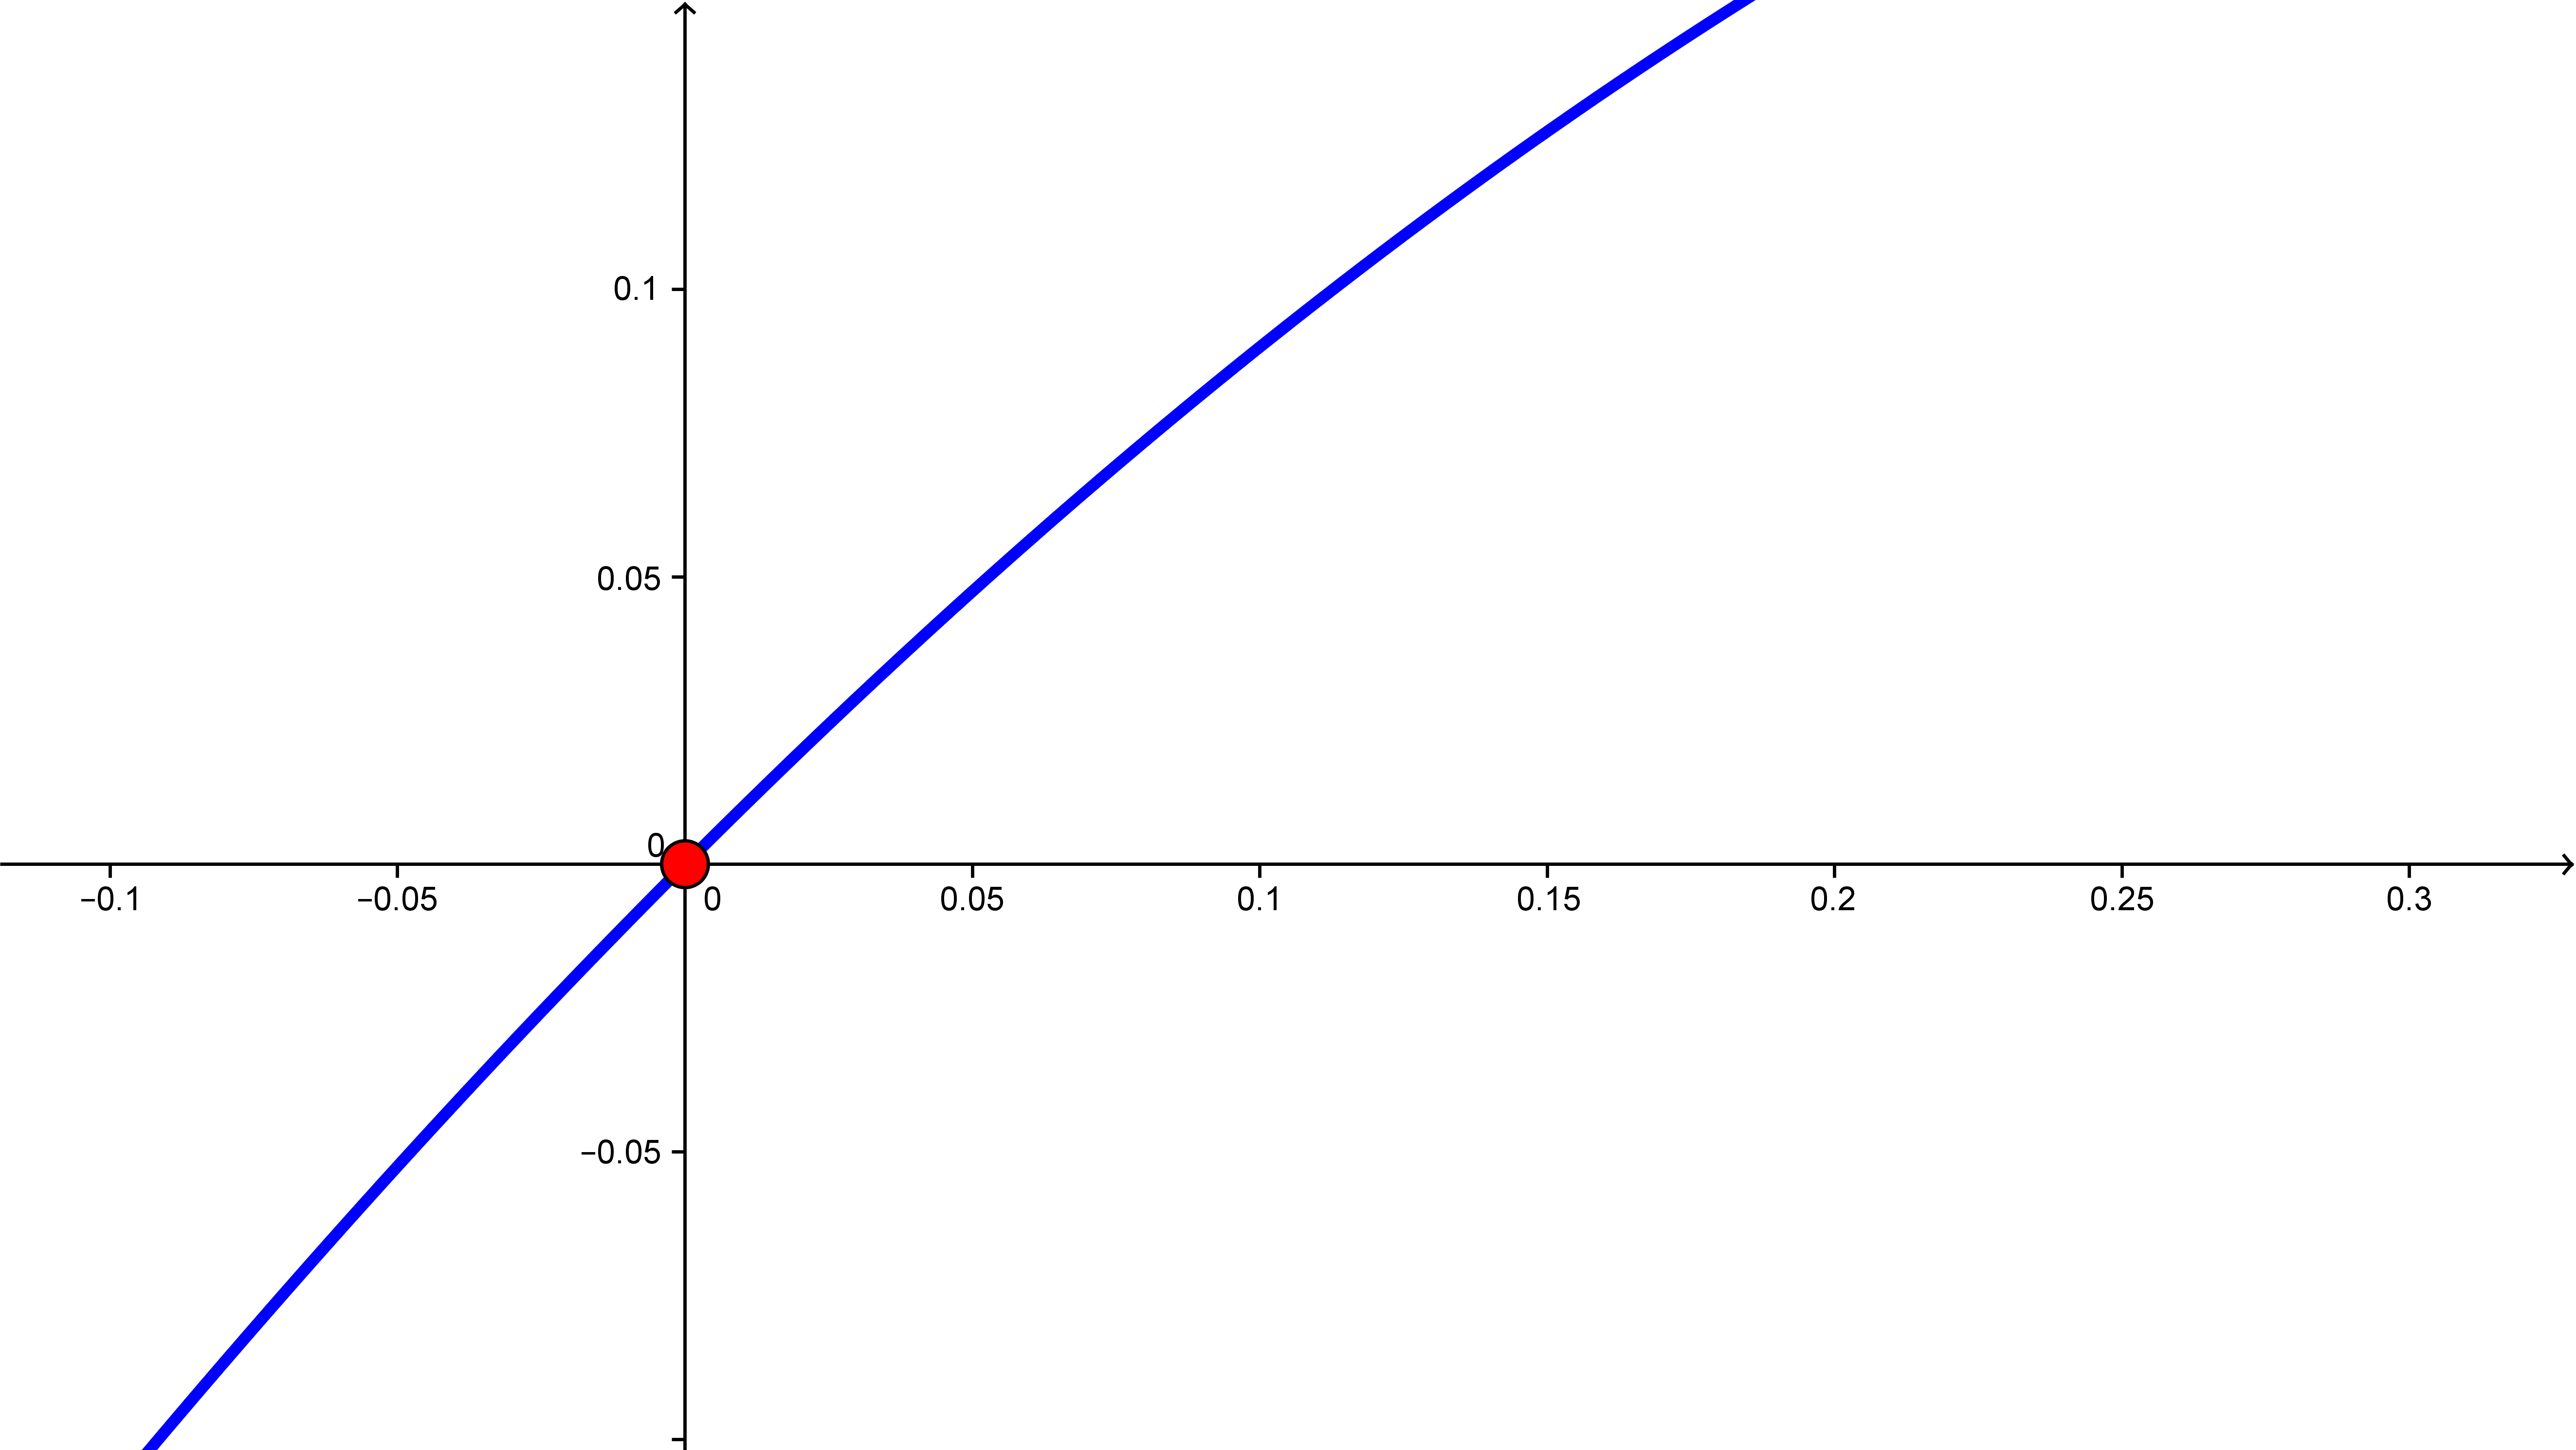
\includegraphics[width=6.5cm]{../fig/Cap10-ZoomEnParabola03.png}&
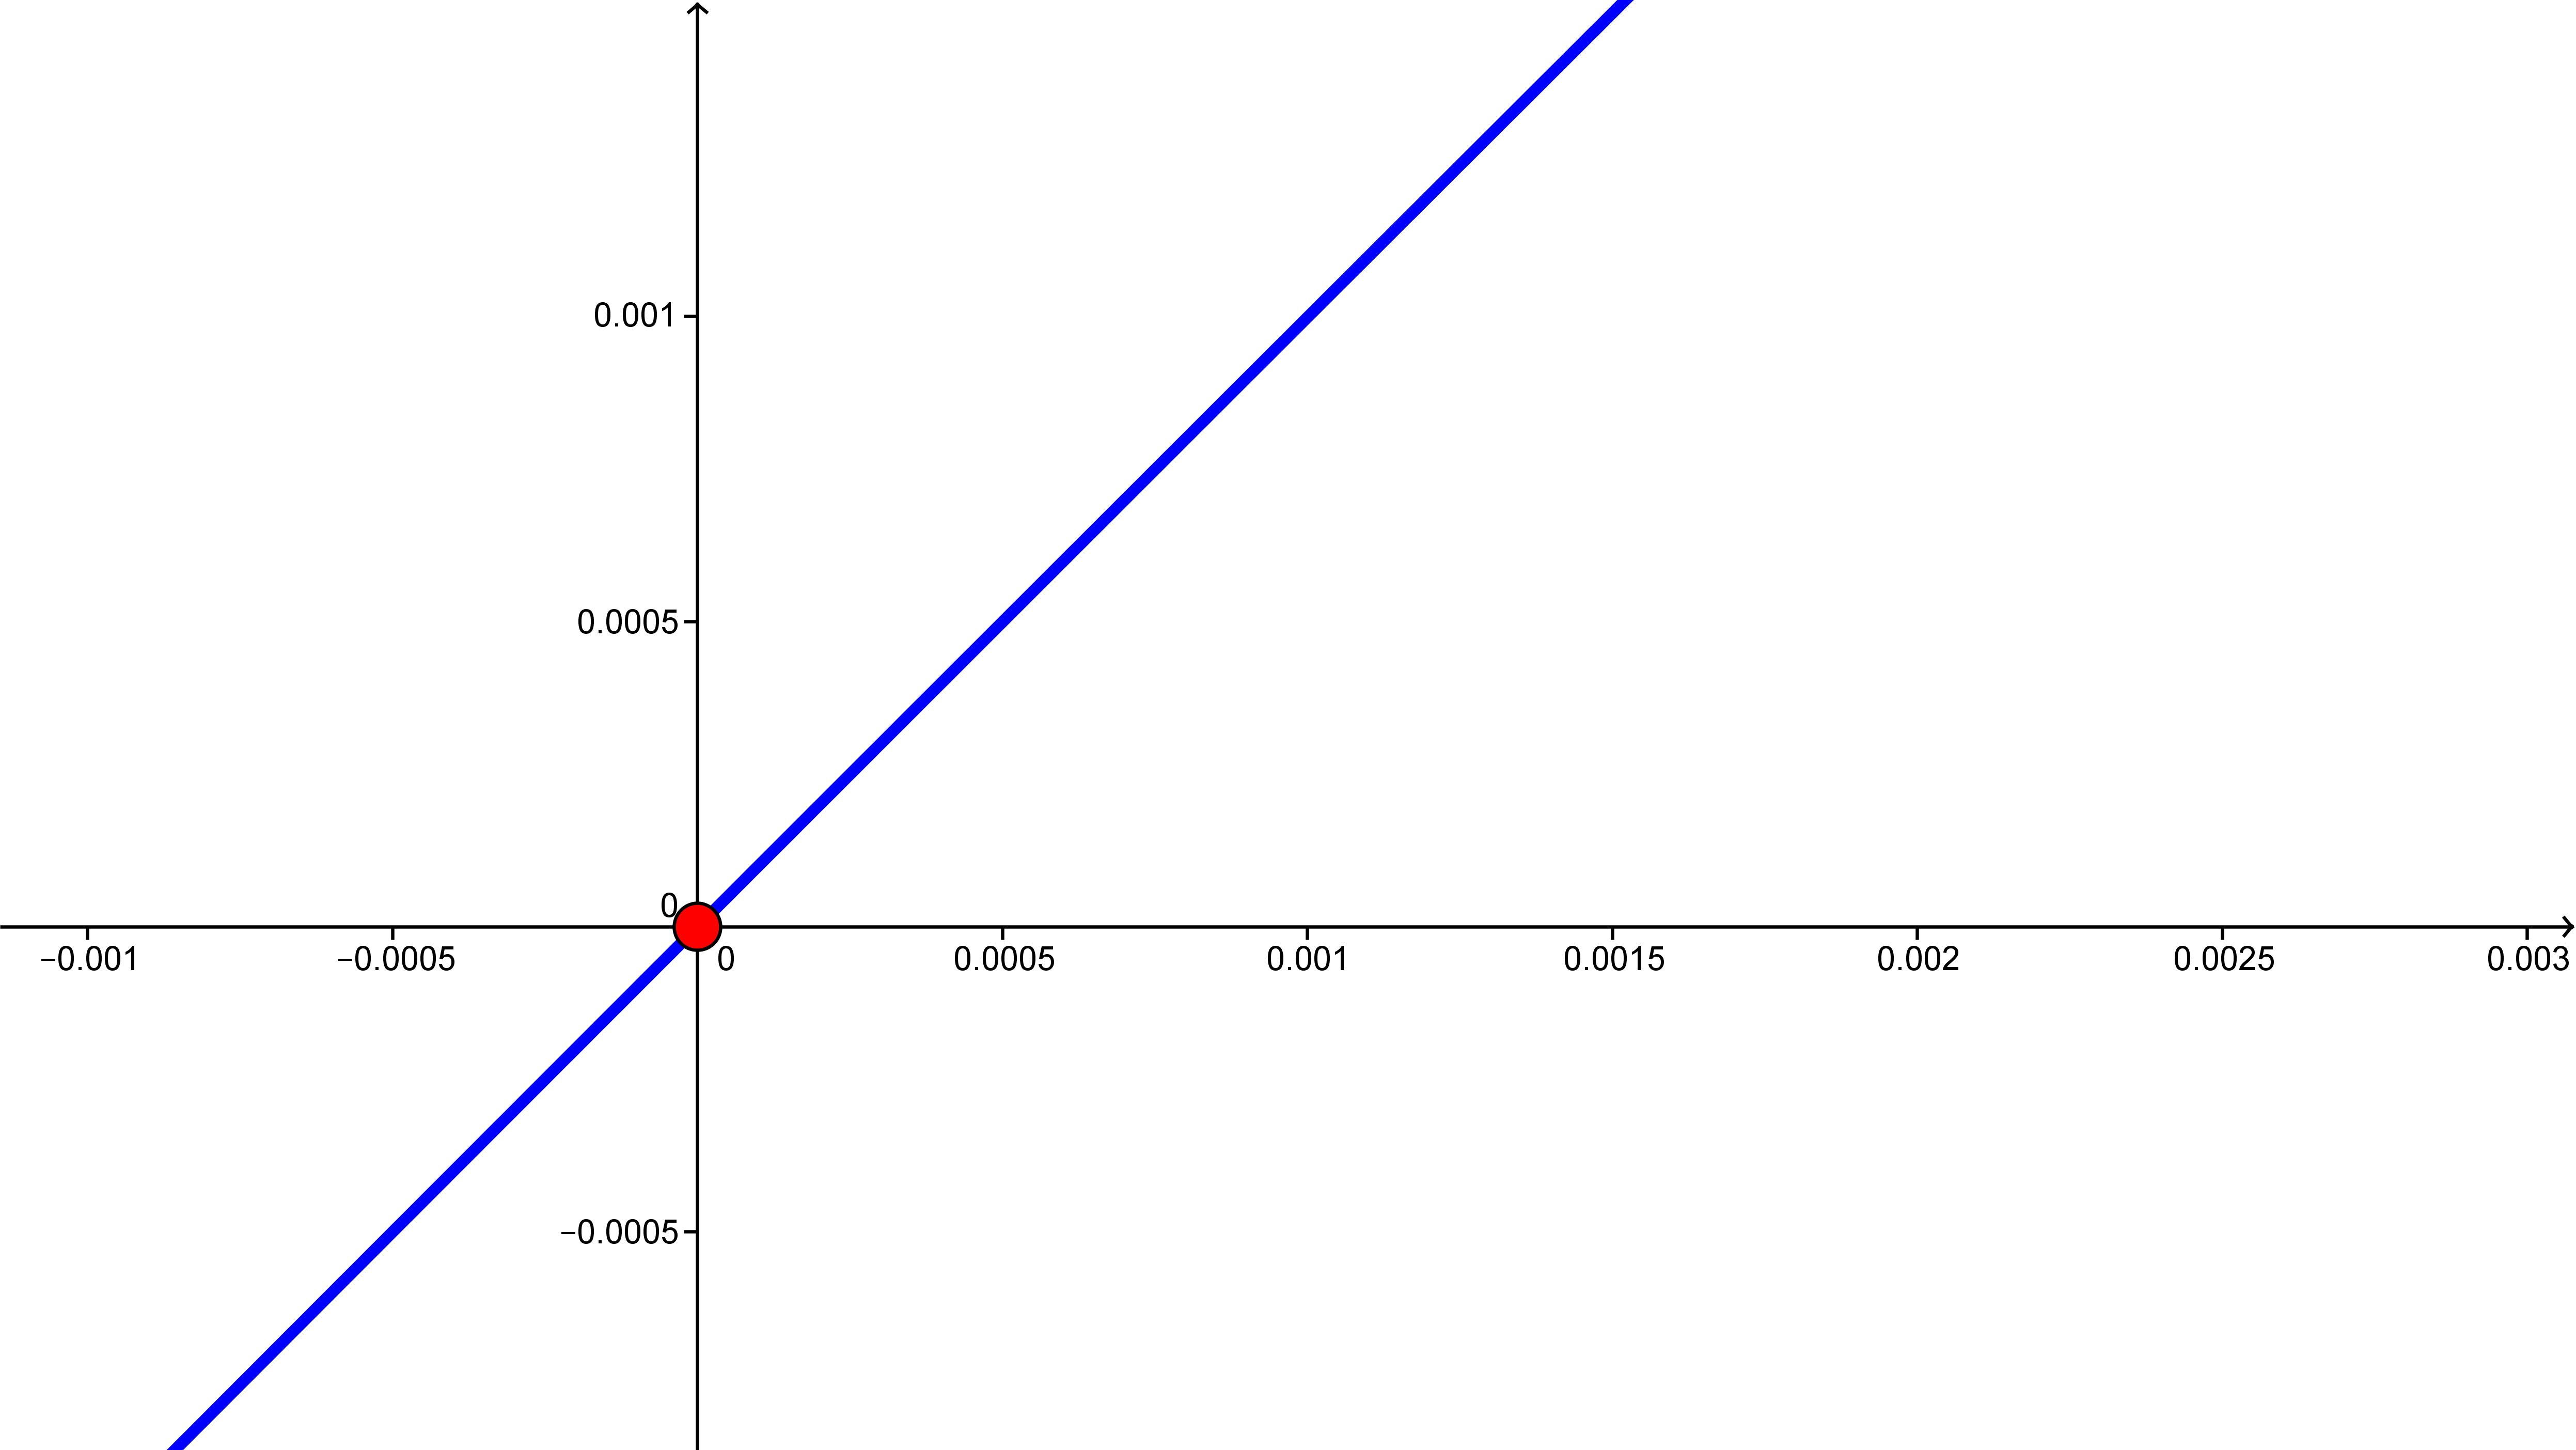
\includegraphics[width=6.5cm]{../fig/Cap10-ZoomEnParabola04.png}\\
(c)&(d)
\end{tabular}
\end{enColor}
\begin{bn}
\begin{tabular}{cc}
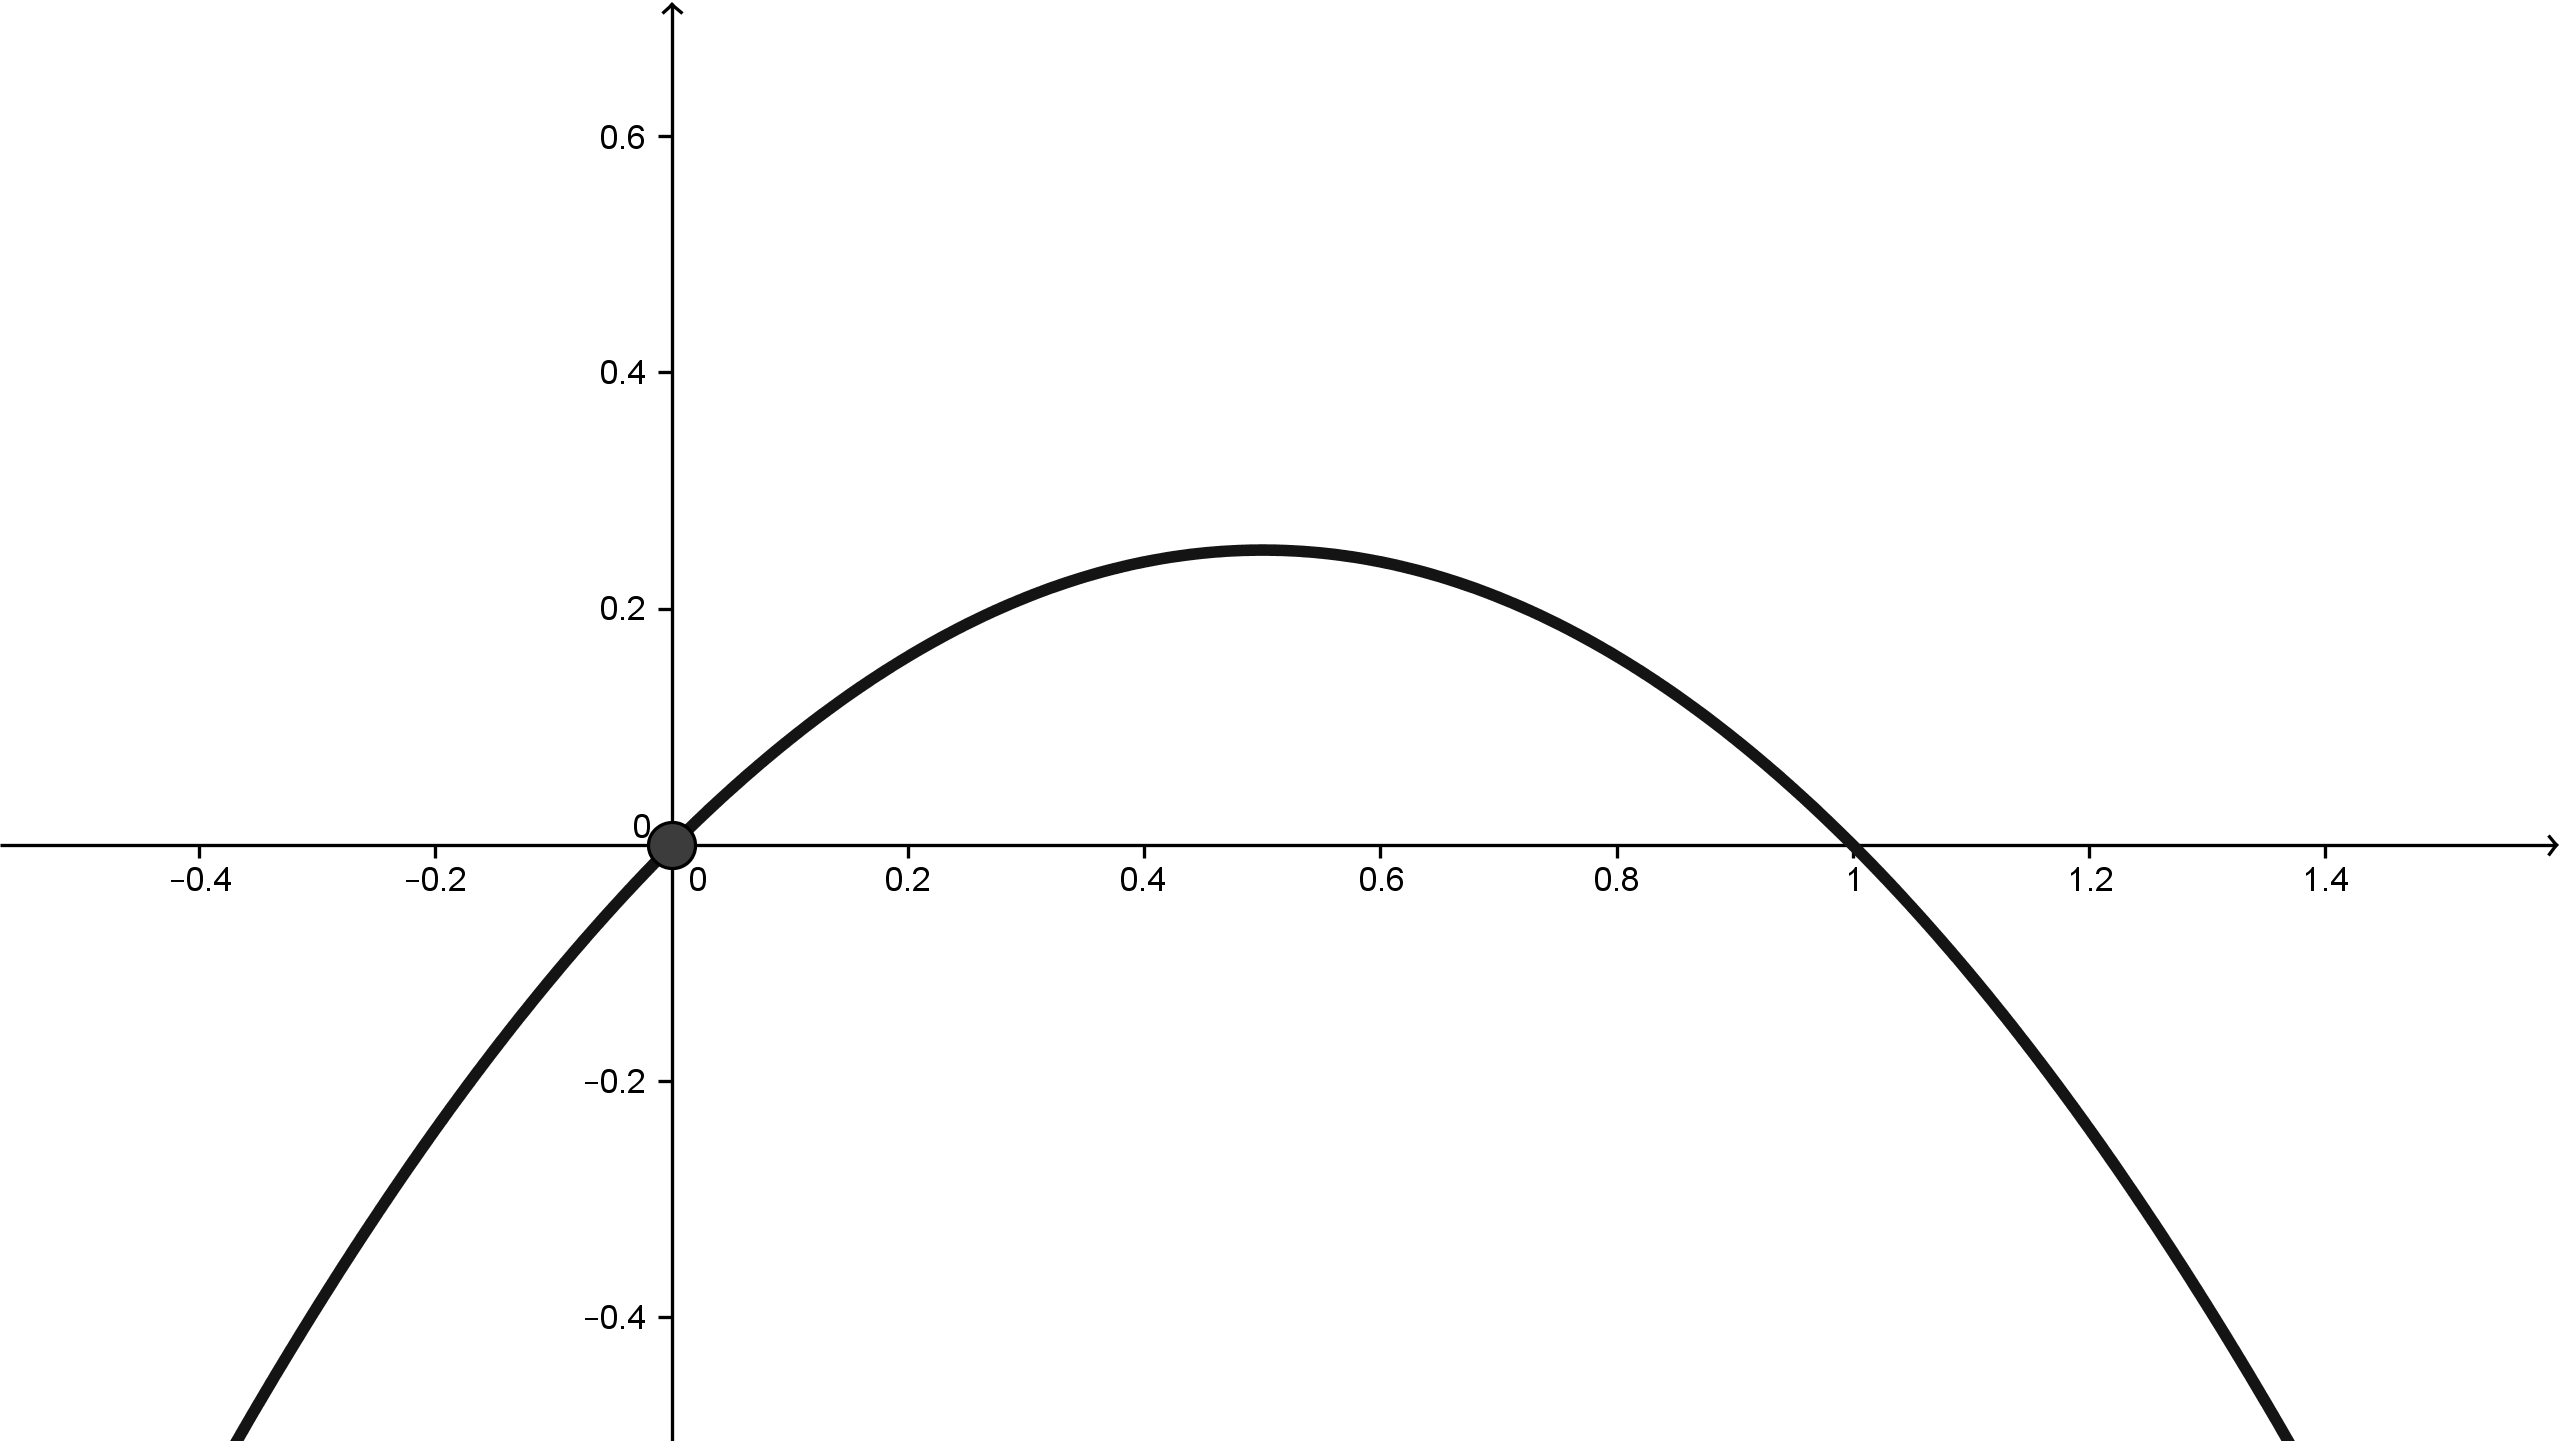
\includegraphics[width=6.5cm]{../fig/Cap10-ZoomEnParabola01-bn.png}&
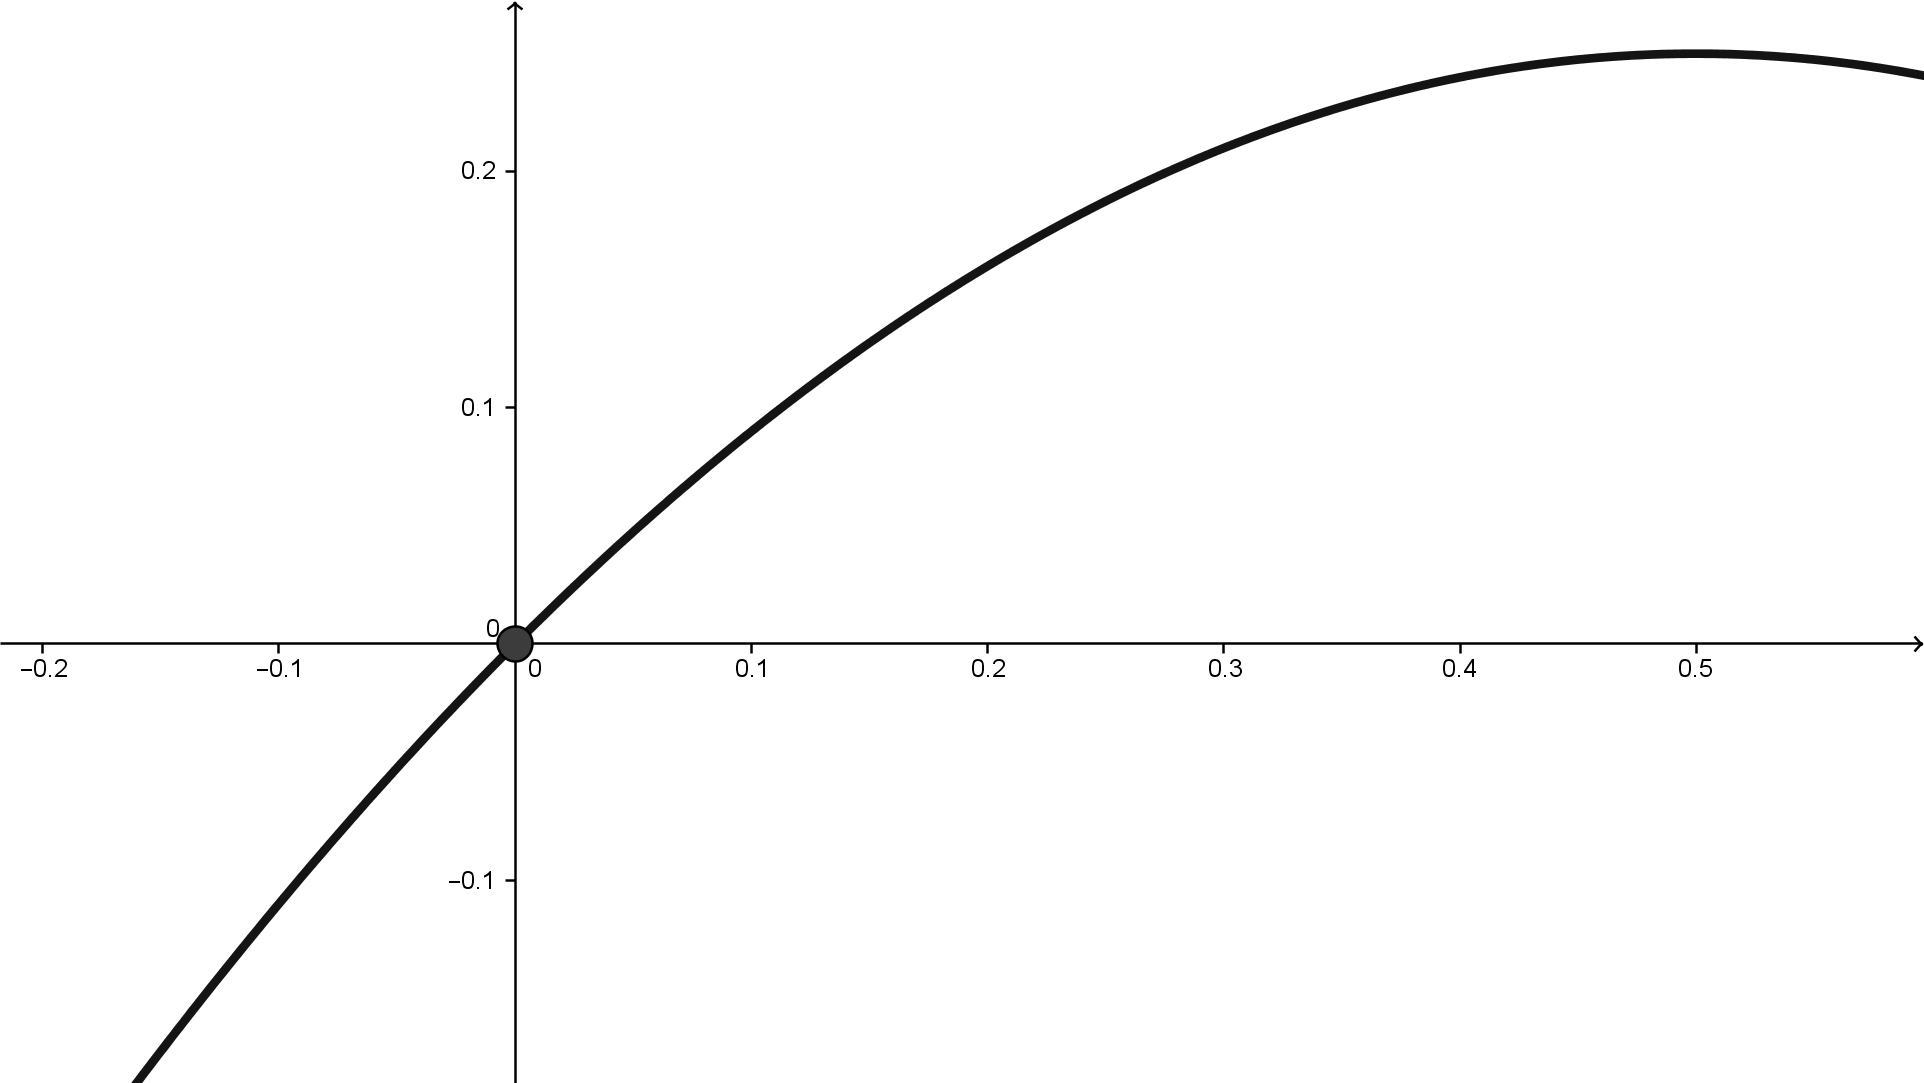
\includegraphics[width=6.5cm]{../fig/Cap10-ZoomEnParabola02-bn.png}\\
(a)&(b)\\
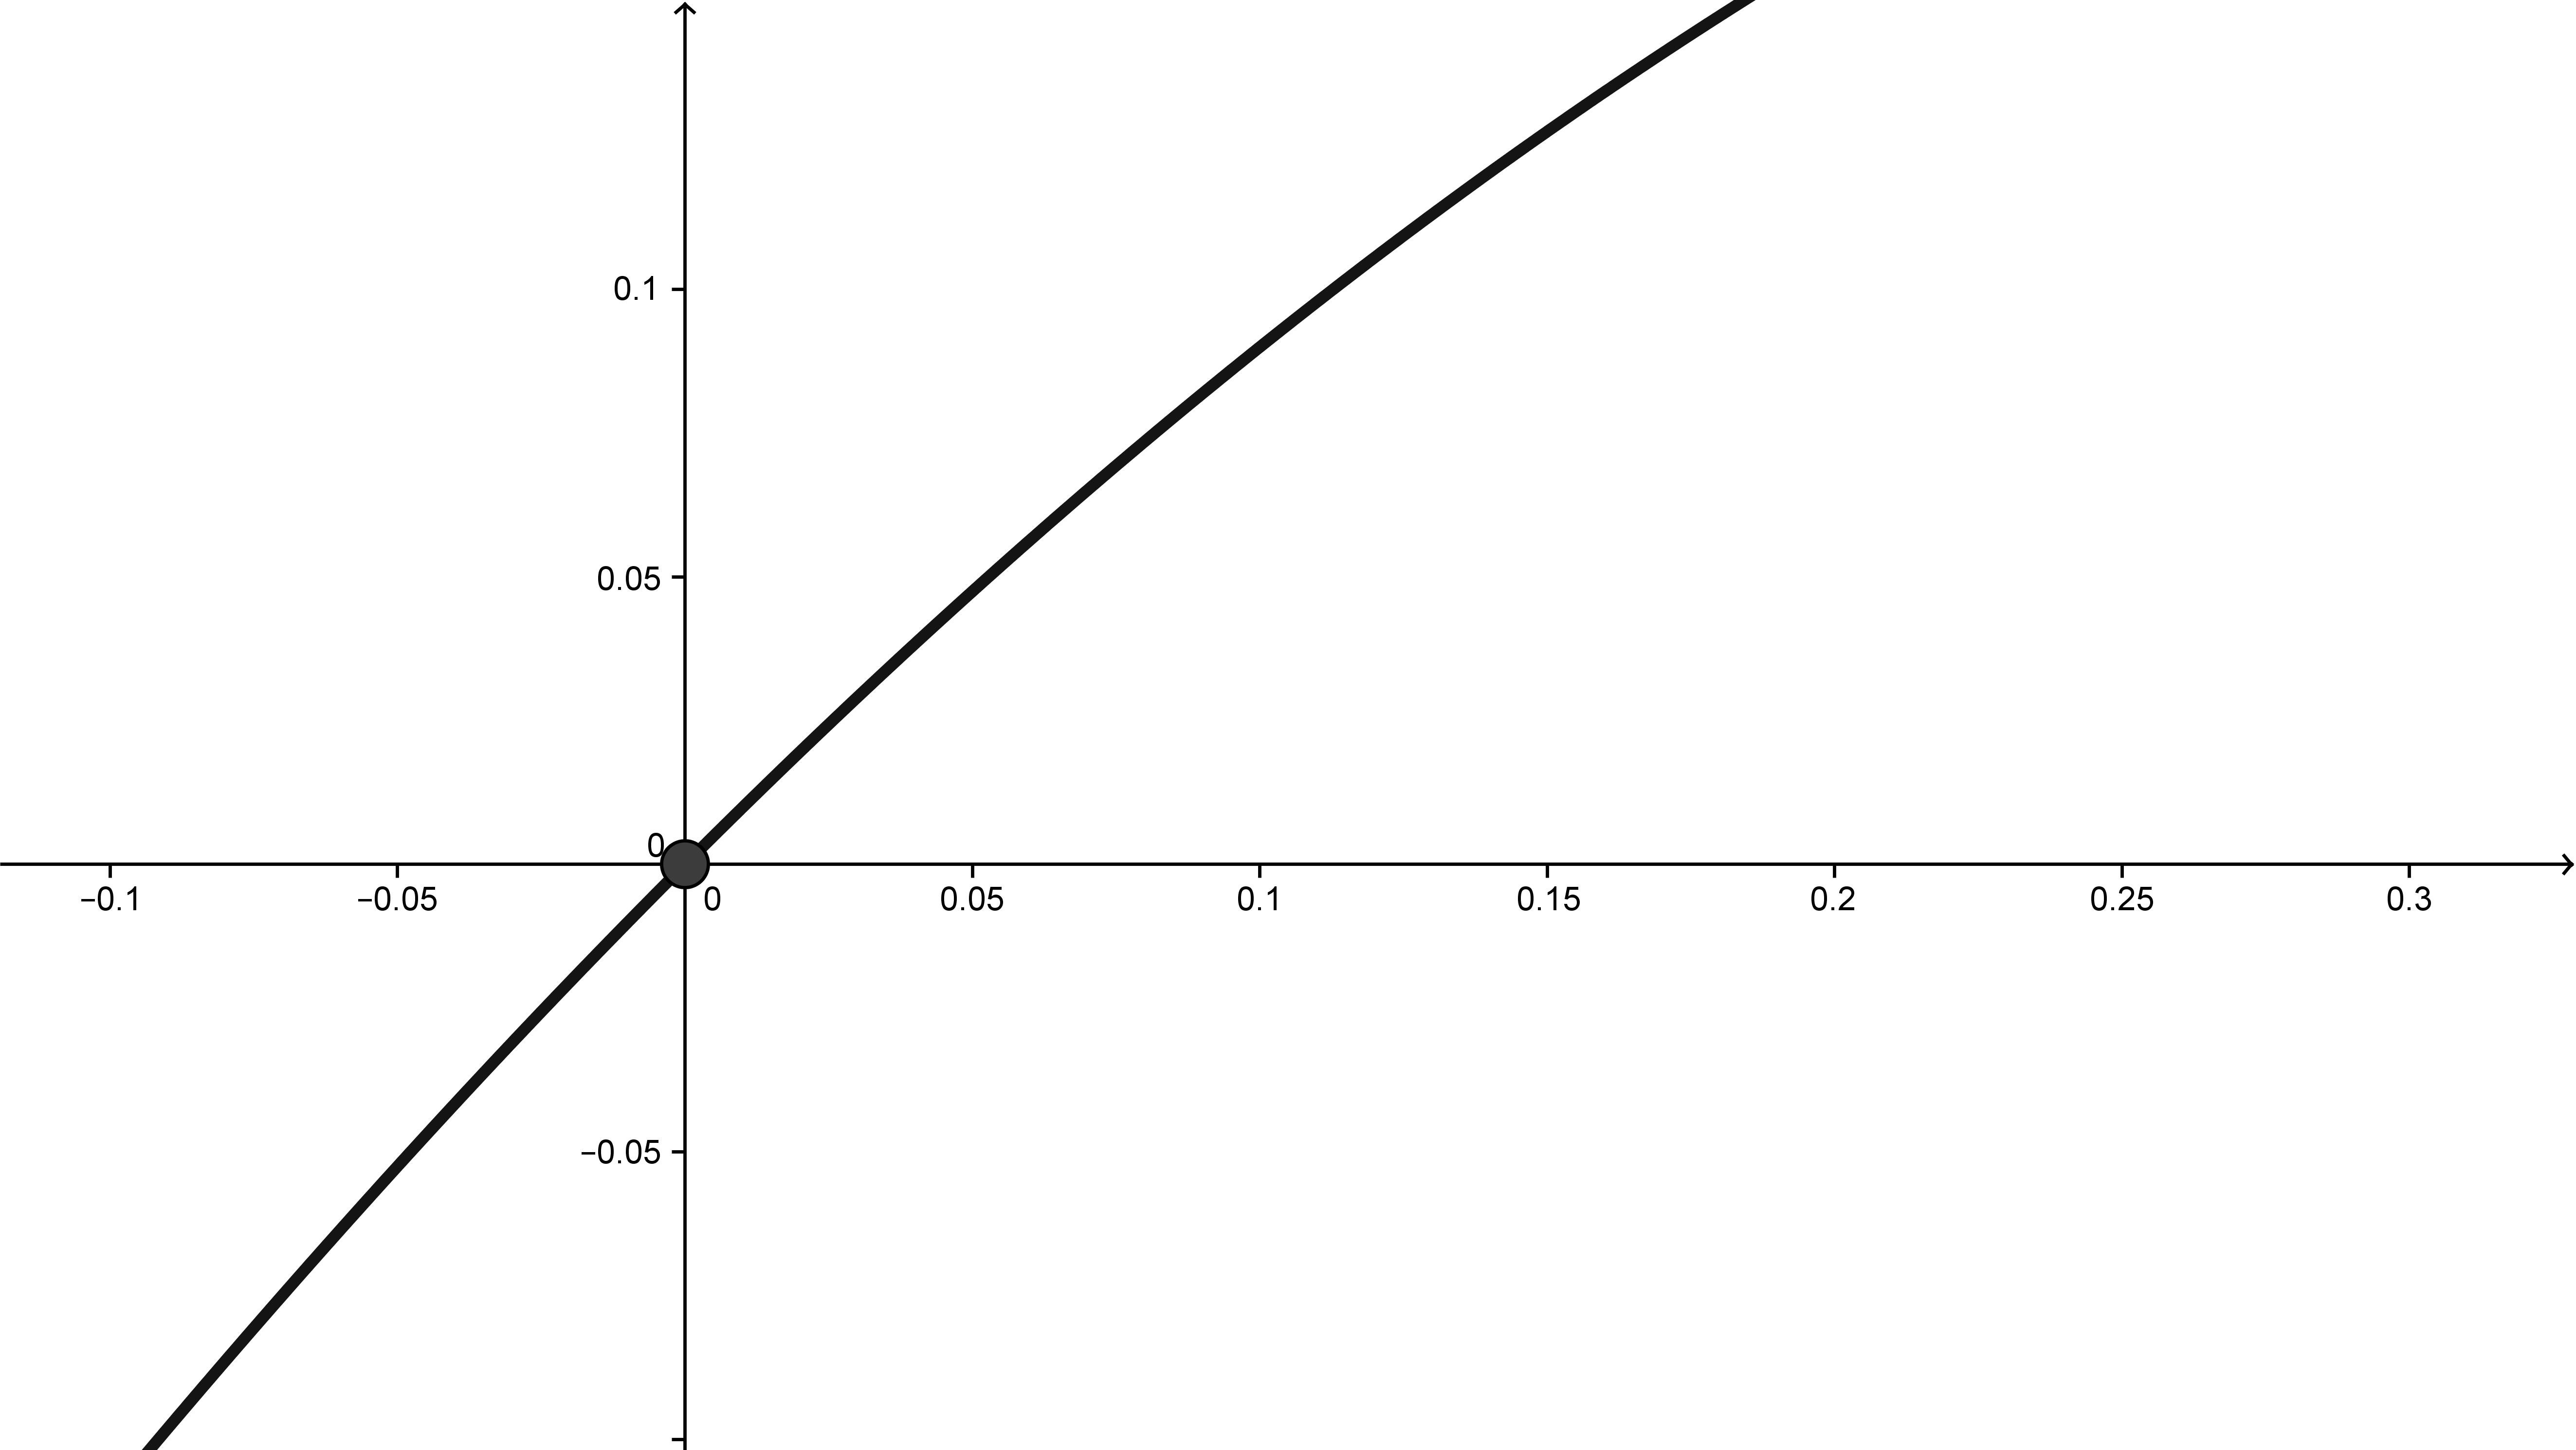
\includegraphics[width=6.5cm]{../fig/Cap10-ZoomEnParabola03-bn.png}&
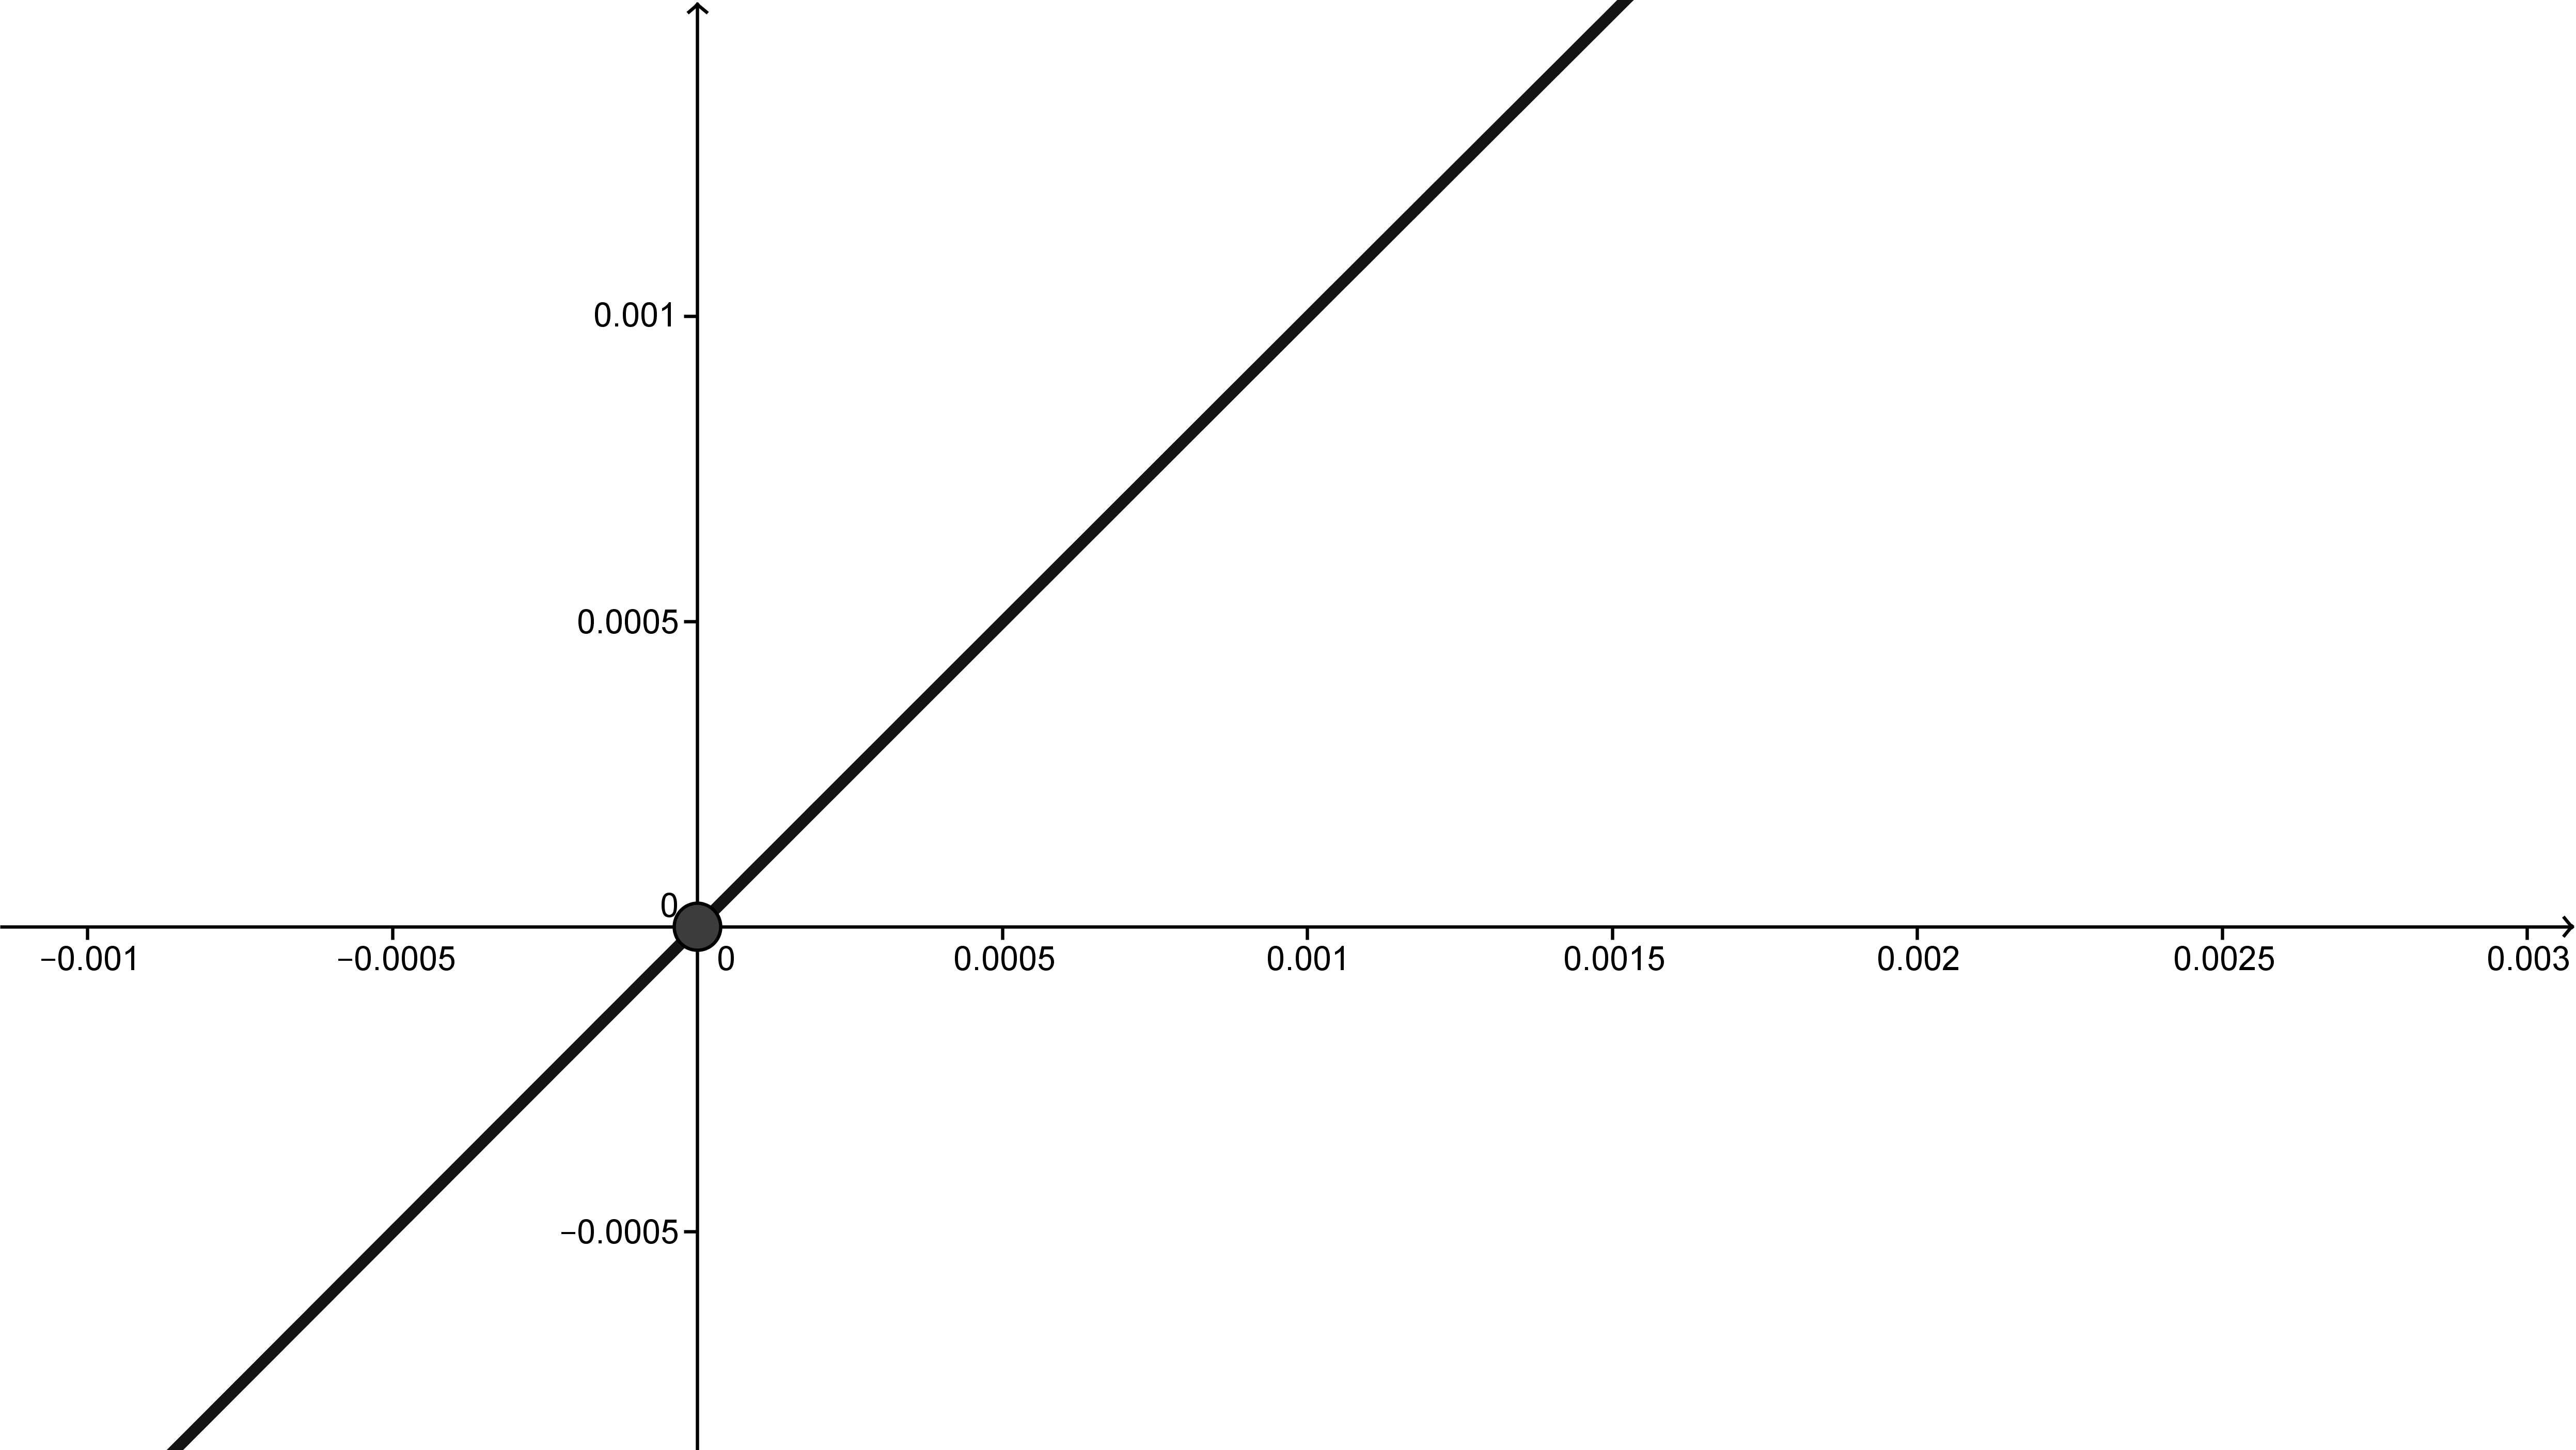
\includegraphics[width=6.5cm]{../fig/Cap10-ZoomEnParabola04-bn.png}\\
(c)&(d)
\end{tabular}
\end{bn}
\caption{La recta como aproximación local, en este caso a la parábola $y=x-x^2$. Al aumentar el zoom en el origen, la parábola se parece cada vez más a su recta tangente en el origen.}
\label{cap10:fig:RectaTangenteParabola}
\end{center}
\end{figure}

Hemos empezado, en la parte (a) de la figura, con la parábola $y=x-x^2$, y hemos ido haciendo zoom en el origen. Al aumentar el zoom en las partes (b), (c) y (d) de la figura se aprecia que la parábola, vista de cerca, se parece cada vez más a cierta recta, de modo que al llegar a una escala de milésimas, en la parte (d) de la figura, la parábola y la recta prácticamente se confunden la una con la otra.

Esa recta que vemos al hacer zoom en punto de la gráfica de una función es, como decíamos, la recta tangente a la función en ese punto. Y el Cálculo Diferencial enseña:
\begin{itemize}
  \item Cómo encontrar esa recta tangente, usando como herramienta la {\sf derivada}.
  \item Las asombrosas aplicaciones de esta idea tan sencilla al estudio de las funciones.
\end{itemize}


%Hemos preparado el fichero GeoGebra \fichero{../datos/Cap10-RectasComoAproximacionLocal.html}{Cap10-RectasComoAproximacionLocal.html }

\begin{figure}[p]
\begin{center}
\begin{enColor}
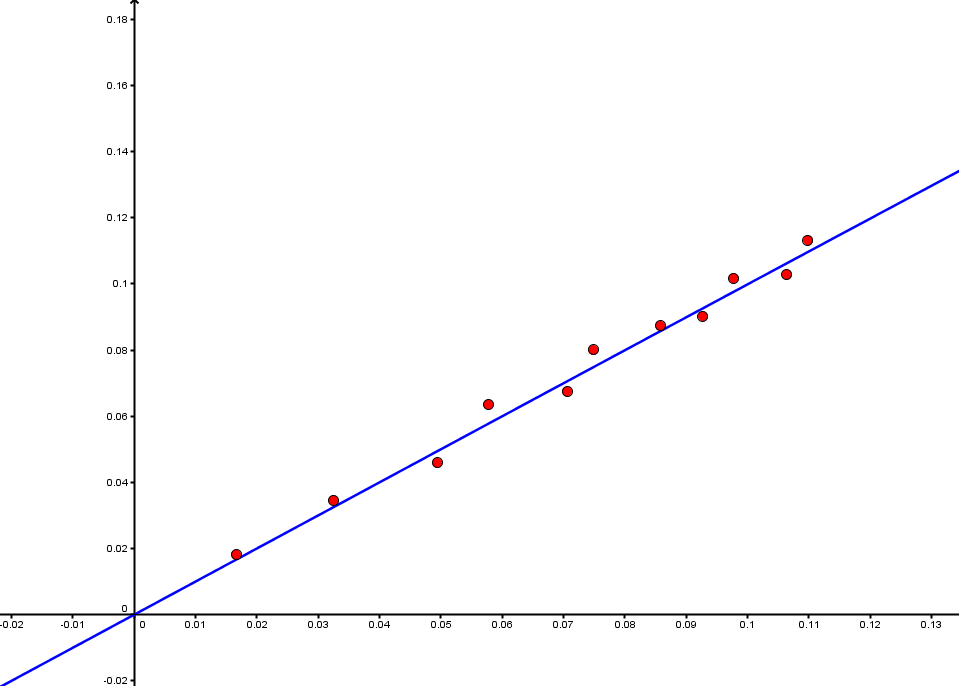
\includegraphics[height=6cm]{../fig/Cap10-EjemploRegresion02a.png}\\
(a) Inicialmente todo parece normal, una recta y unos puntos.\\
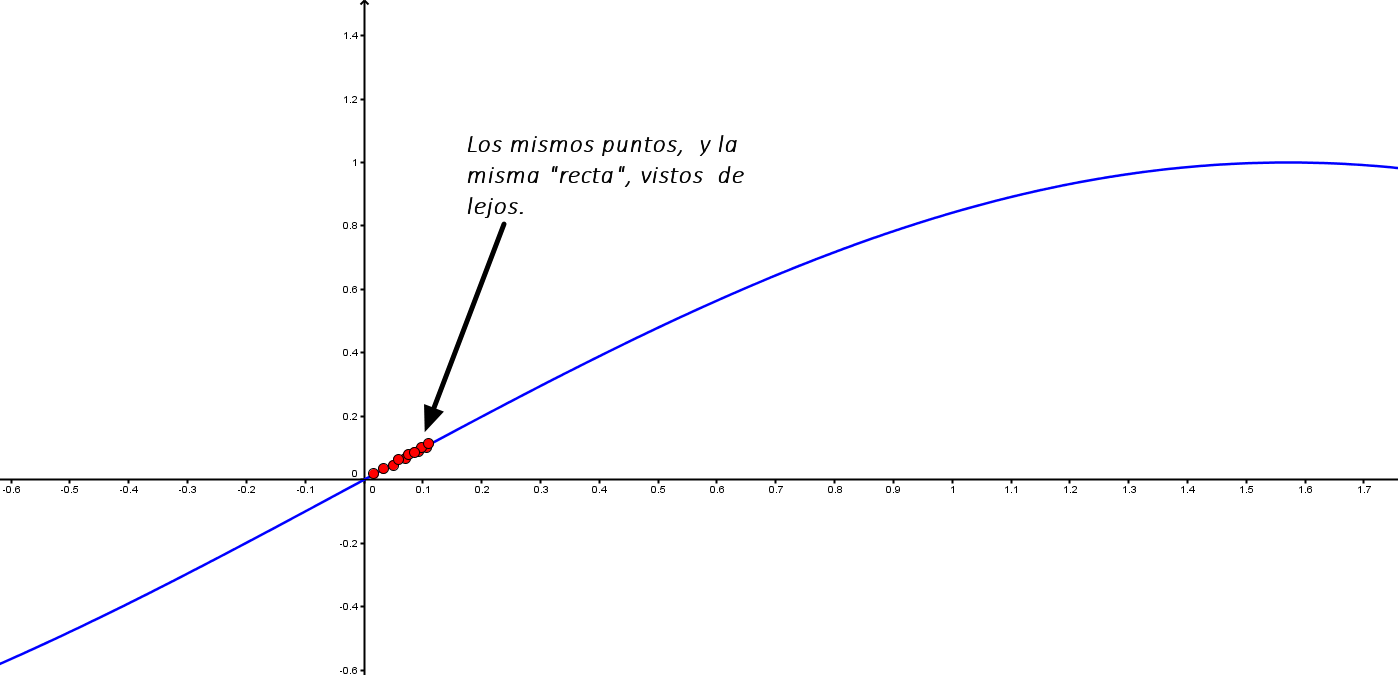
\includegraphics[height=6cm]{../fig/Cap10-EjemploRegresion02b.png}\\
(b) Pero al hacer zoom hacia fuera, la recta cambia.
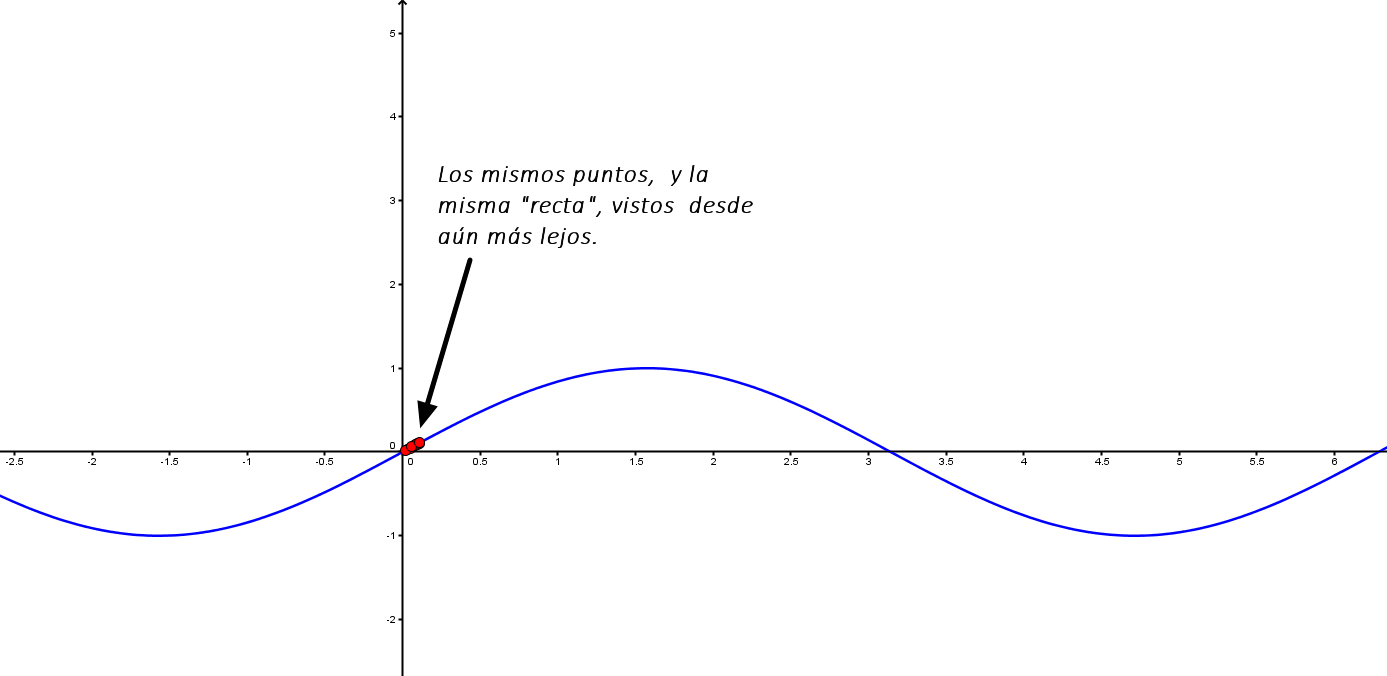
\includegraphics[height=6cm]{../fig/Cap10-EjemploRegresion02c.png}\\
(c) Y ahora ya est\'a claro lo que sucede. No hay tal recta.
\end{enColor}
\begin{bn}
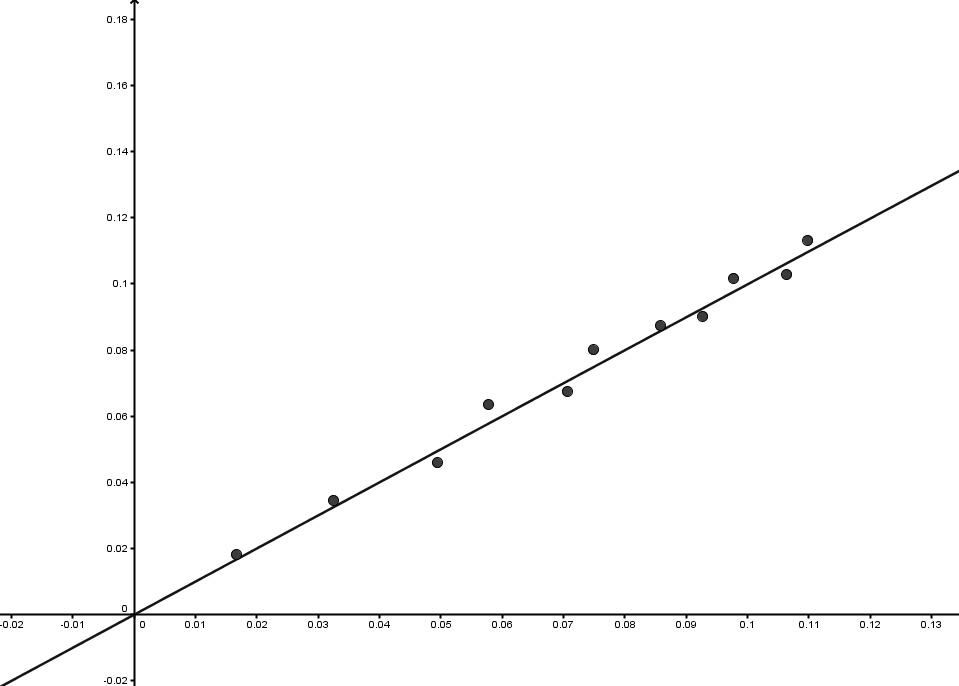
\includegraphics[height=6cm]{../fig/Cap10-EjemploRegresion02a-bn.png}\\
(a) Inicialmente todo parece normal, una recta y unos puntos.\\
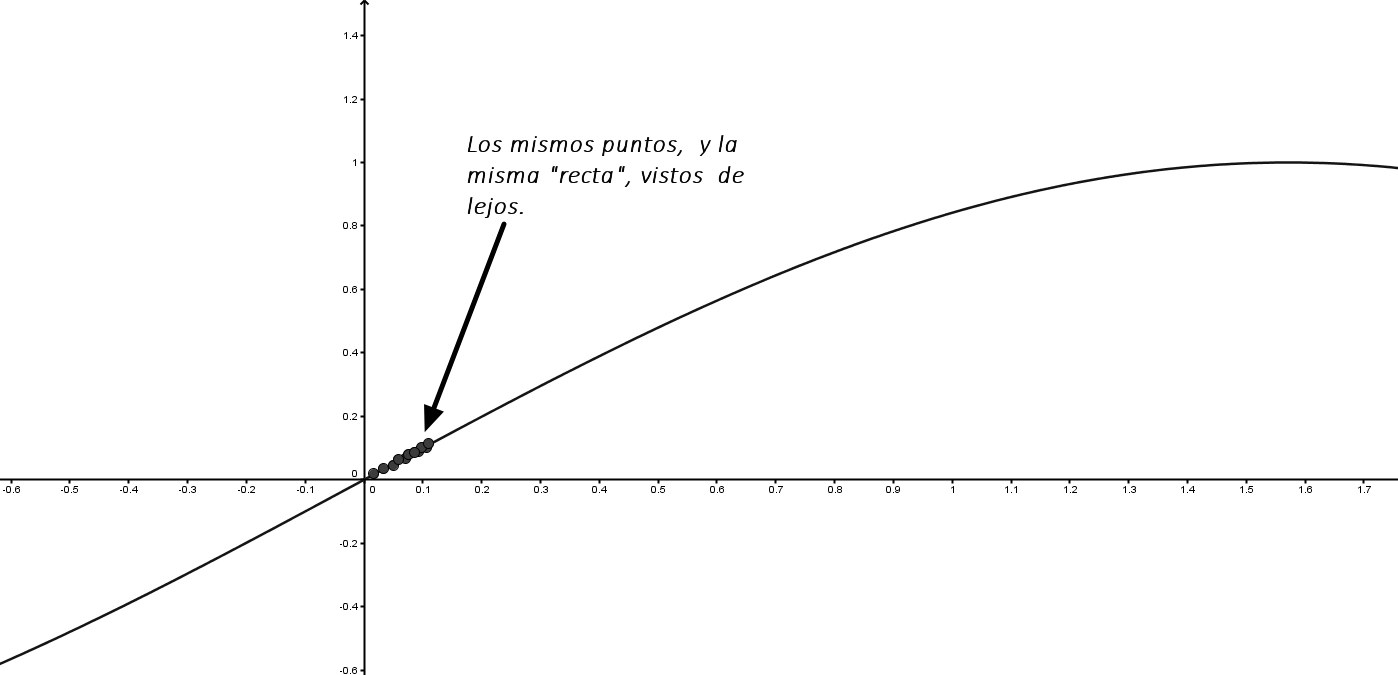
\includegraphics[height=6cm]{../fig/Cap10-EjemploRegresion02b-bn.png}\\
(b) Pero al hacer zoom hacia fuera, la recta cambia.
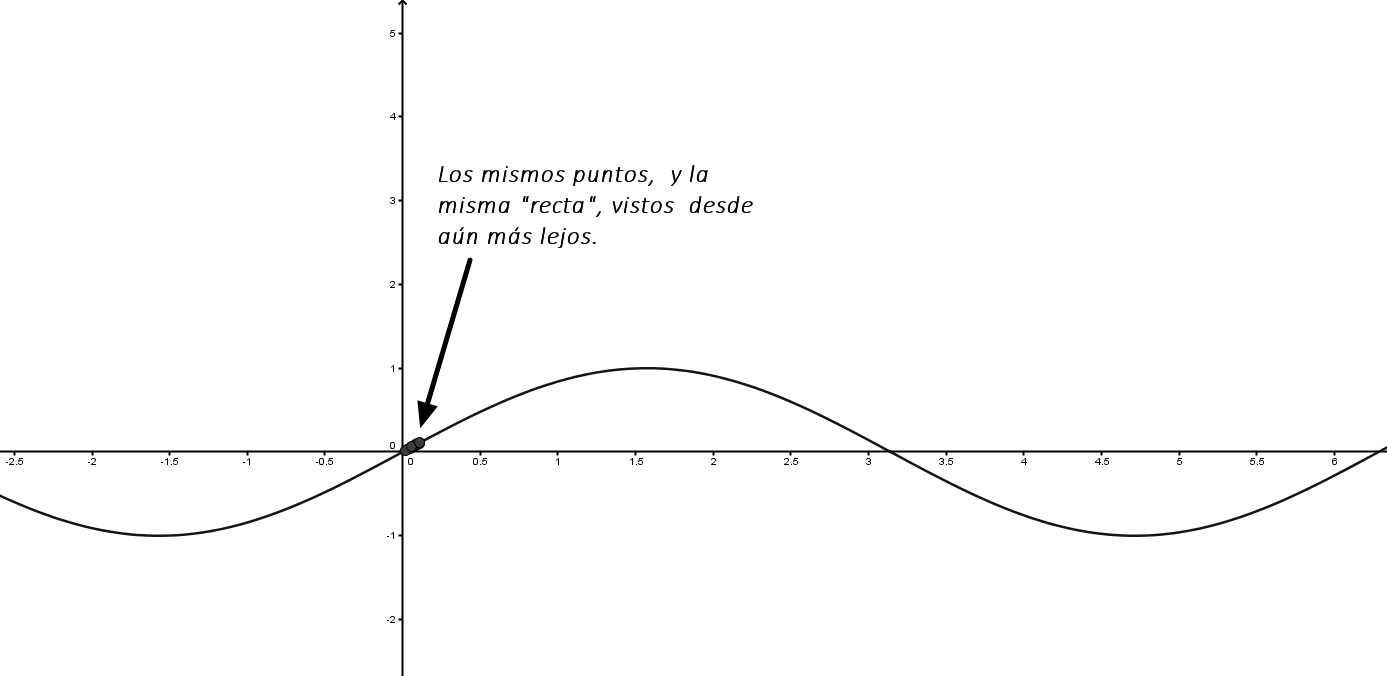
\includegraphics[height=6cm]{../fig/Cap10-EjemploRegresion02c-bn.png}\\
(c) Y ahora ya est\'a claro lo que sucede. No hay tal recta.
\end{bn}
\caption{La recta como aproximación local a una función.}
\label{cap10:fig:RectaComoAproximacionLocal}
\end{center}
\end{figure}

Si el {\em ``zoom hacia dentro''} en la gráfica de una función nos permite intuir la idea de recta tangente, no es menos cierto que el {\em ``zoom hacia fuera''} guarda también una lección muy importante. Tenemos que ser conscientes de que, al mirar algo que parece una recta, podemos estar mirándolo a una escala demasiado pequeña. Al alejarnos, a menudo descubrimos que el fenómeno que estamos estudiando es más complejo de lo que parecía. Esto se ilustra en  la Figura \ref{cap10:fig:RectaComoAproximacionLocal}: en esa figura empezamos con algo que parece una recta y, al alejarnos, descubrimos que en realidad lo que estábamos mirando era una función trigonométrica (concretamente, la función seno). Como hemos dicho, en el Tutorial10 tendremos ocasión de usar el ordenador para poner en práctica esta idea del ``zoom'' hacia dentro a hacia fuera en la gráfica de una función.
%En el fichero GeoGebra \fichero{../datos/Cap10-ZoomEnParabola.html}{Cap10-ZoomEnParabola.html}, y en

Volviendo a la Estadística, y al problema de la recta de regresión, resumimos nuestros hallazgos: lo importante, para nosotros, de este descubrimiento es que, cuando se estudia la dependencia entre dos variables {\em en un intervalo reducido, muy local, de valores}, lo previsible es encontrar una recta. Pero también es importante aprender la lección inversa: lo que a cierta escala parece una recta, puede ser sólo una visión demasiado local, demasiado limitada, de la verdadera relación entre las dos variables, que puede ser mucho más compleja de lo que una simple recta es capaz de representar.

\subsubsection*{Extrapolación.}
\label{cap10:subsubsec:Extrapolacion}

En particular, estas observaciones sirven también para alertarnos sobre un peligro inherente al uso de la recta de regresión. Supongamos que tenemos los datos
        \[(x_1,y_1),\ldots,(x_n,y_n)\]
        y sean
        \[
        \begin{cases}
        m_x=\min(x_1,\ldots,x_n)\\
        M_x=\max(x_1,\ldots,x_n)
        \end{cases}
        \]

    \begin{center}
    \fcolorbox{black}{Gris025}{
    \begin{minipage}{13.5cm}
        {\bf Nunca, bajo ningún concepto}, está justificado el uso de la recta para predecir valores de $y$ correspondientes a valores de $x$ fuera del intervalo $(m_x,M_x)$. Hacer eso se denomina {\sf extrapolación}\index{extrapolación}, y se considera uno de los errores más graves que pueden cometerse en el contexto del uso de la recta de regresión.
       %%%%%%%%%%%%%%%%%%%%%%%%%%%%%%%%%%%%%%%
    \end{minipage}
    }
    \end{center}
La razón por la que la extrapolación es un error debería estar clara a partir de la discusión precedente: si hiciéramos eso estaríamos usando la recta en una zona en la que el fenómeno puede tener un comportamiento muy alejado del que predice esa recta.

Más allá de esta advertencia genérica sobre la extrapolación, volveremos con más detalle sobre el tema de la predicción en la Sección \ref{cap10:subsec:BandasConfianzaPrediccion} (pág. \pageref{cap10:subsec:BandasConfianzaPrediccion}).

\subsection{Regresión ortogonal.}
\label{cap10:subsec:RegresionOrtogonal}
\noindent{\bf Opcional: esta sección puede omitirse en una primera lectura.}\\

Antes de seguir adelante, y de que los detalles técnicos se crucen en nuestro camino, queremos detenernos en un punto que, por sutil, puede pasar inadvertido. Pero que será muy importante más adelante, en el Capítulo \ref{cap:RegresionLogistica}, cuando hablemos de modelos lineales generalizados.

En todo lo que hemos hecho ahora hemos supuesto que el punto de partida es una muestra de puntos, como:
\[(x_1, y_1),\, (x_2, y_2),\, (x_3, y_3),\, \ldots,\, (x_n, y_n).\]
Y de ahí hemos pasado a los puntos predichos por el modelo:
\[(x_1, \hat y_1),\, (x_2,\hat y_2),\, (x_3, \hat y_3),\, \ldots,\, (x_n, \hat y_n).\]
Pero en ambos casos los valores de las primeras coordenadas, $x_1, \ldots, x_n$ eran los mismos. Al hacer esto, de manera implícita (y por eso es sutil), estamos dando por sentado que esos valores de $x$ están fijos o, dicho de otro modo, vienen dados. En muchas ocasiones, eso será así. En un experimento sobre las propiedades de un gas podemos, por ejemplo, fijar los valores $x$ de la temperatura, y estudiar los correspondientes valores $y$ de la presión (por poner un ejemplo). Este tipo de situaciones describen lo que se conoce como {\sf regresión de tipo I}\index{regresión tipo I vs tipo II}\index{tipo I vs tipo II, regresión}.

En otras situaciones, las cosas serán distintas. En situaciones como las del ejemplo de la hembra de {\em Herrerillo} incubando, está claro que los científicos no han {\em fijado} la temperatura, sino que han {\em observado} la temperatura que hacía cada día durante el estudio. Es decir, que los valores de la variable $x$ son valores aleatorios. Este segundo tipo de situaciones corresponde con lo que a veces se llama {\sf regresión de tipo II}. En principio, podemos tratar los dos tipos de situaciones con las mismas herramientas matemáticas, y así se hace, de hecho, en muchos casos. Pero es muy importante entender la diferencia, y las alternativas a nuestro alcance.

Si suponemos que los valores de $x$ no están fijos, entonces, cuando tomemos otra muestra de $n$ puntos obtendremos
\[(x'_1, y'_1),\, (x'_2, y'_2),\, (x'_3, y'_3),\, \ldots,\, (x'_n, y'_n),\]
donde las primas (') indican que tanto los valores de $x$ como los de $y$ son distintos de los anteriores. ¿Qué sentido tiene, en casos como estos, hablar de los valores que {\em predice} el modelo? Para hablar de predicción, en estos casos, resulta adecuado asumir que tendremos que predecir tanto los valores de la $x$ como los de la $y$. Es decir, que en este caso, al hablar de predicciones, ya no pensamos sólo en predecir los valores $\hat y_1, \ldots, \hat y_n$ como hacíamos antes. Ahora pensamos en los puntos predichos en esta  forma:
\begin{equation}
\label{cap10:ecu:ValoresPredichosModeloIIRegresion}
(\hat x_1, \hat y_1),\, (\hat x_2,\hat y_2),\,  \ldots,\, (\hat x_n, \hat y_n),
\end{equation}
donde ambas coordenadas forman parte del proceso de predicción.

¿Qué cambia con esto? Pues, por ejemplo, pero de forma destacada, nuestra visión de la forma de definir la que hemos definido como ``la mejor recta posible''. Para entenderlo, es esencial volver a pensar en la situación de la Figura \ref{cap10:fig:InterpretacionErrorCuadratico} (pág. \pageref{cap10:fig:InterpretacionErrorCuadratico}). Esa figura ilustra la interpretación geométrica del error cuadrático $EC$, que se define a partir de las diferencias (residuos)
\[e_i = y_i - \hat y_i.\]
El valor de $x$ no interviene al definir el residuo porque (y este es el punto clave) los valores de $x$ se consideran fijos. Pero si suponemos que el valor de $\hat x_i$ es distinto de $x_i$, esto no tiene mucho sentido.

¿Y entonces qué hacemos, cómo definimos la ``mejor recta'' si los valores de $x$ no son fijos? Para llegar a la respuesta debemos  recordar que seguimos buscando una recta y, en particular, los puntos \ref{cap10:ecu:ValoresPredichosModeloIIRegresion} son puntos de esa recta.  En particular, el punto $(\hat x_i, \hat y_i)$ es el punto de la recta que {\em corresponde} al punto $(x_i, y_i)$ de la muestra. Hemos destacado la palabra ``corresponde'' porque de eso se trata, precisamente. Veámoslo en detalle. Cuando usábamos los residuos para definir el error cuadrático, pasábamos del punto $(x_i, y_i)$ de la muestra al punto predicho $(x_i, \hat y_i)$, moviéndonos en vertical (la coordenada $x$ está fija). Aunque en ese momento puede haber parecido una elección natural, está claro, a la luz de nuestra presente discusión, que esa elección tiene mucho que ver con lo que hemos llamado modelo I de regresión.

Así que, volviendo a la pregunta de cómo debemos elegir la mejor recta, ahora vemos que el primer paso depende de la respuesta a esta otra pregunta. Dado un punto $(x_i, y_i)$, ¿cuál es el punto {\em correspondiente} $(\hat x_i, \hat y_i)$ de la recta? Hay varias formas de responder, que en general se reducen a elegir la forma de movernos desde $(x_i, y_i)$ hasta la recta: podemos movernos en vertical hasta llegar a la recta, que es lo que hemos hecho hasta ahora. O podemos movernos en horizontal (cuando usamos valores fijos de $y$ para predecir los valores de $x$).
%\textcolor{red}{eso no es cambiarde ejes?}
O podemos movernos {\em por el camino más corto}. Esta última opción es especialmente interesante, y se corresponde con lo que se denomina a veces como {\sf regresión ortogonal}\index{regresión ortogonal}\index{regresión ortogonal}\index{ortogonal, regresión} (en inglés la terminología estándar es  {\em major axis regression}\index{major axis regression}\index{regression, major axis}). Veamos un ejemplo.

\begin{ejemplo}
\label{cap10:ejem:regresionMAR}
Supongamos que, de forma similar al Ejemplo \ref{cap10:ejem:Regresion01} (pág. \pageref{cap10:ejem:Regresion01}),  tenemos $n=10$ puntos $(x_i,y_i)$, definidos en la Tabla \ref{cap10:tabla:EjemploRegresionMAR}. En la Figura \ref{cap10:fig:RegresionMAR} se muestra el correspondiente diagrama de dispersión, con dos rectas de regresión obtenidas por métodos distintos.
\begin{table}[ht]
\centering
\begin{tabular}{rrrrrrrrrrr}
  \hline
 & 1 & 2 & 3 & 4 & 5 & 6 & 7 & 8 & 9 & 10 \\
  \hline
$x$ & 1.14& 3.3& 5.38& 5.8& 5.96& 5.97& 6.2& 6.38& 9.06& 11.45 \\
$y$ & 4.83& 2.76& 4.85& 3.47& 1.82& 6.74& 3.6& 9.7& 5.95& 8.72 \\
   \hline
\end{tabular}
\caption{Datos del Ejemplo \ref{cap10:ejem:regresionMAR}.}
\label{cap10:tabla:EjemploRegresionMAR}
\end{table}

\begin{figure}[htbp]
\begin{center}
\begin{enColor}
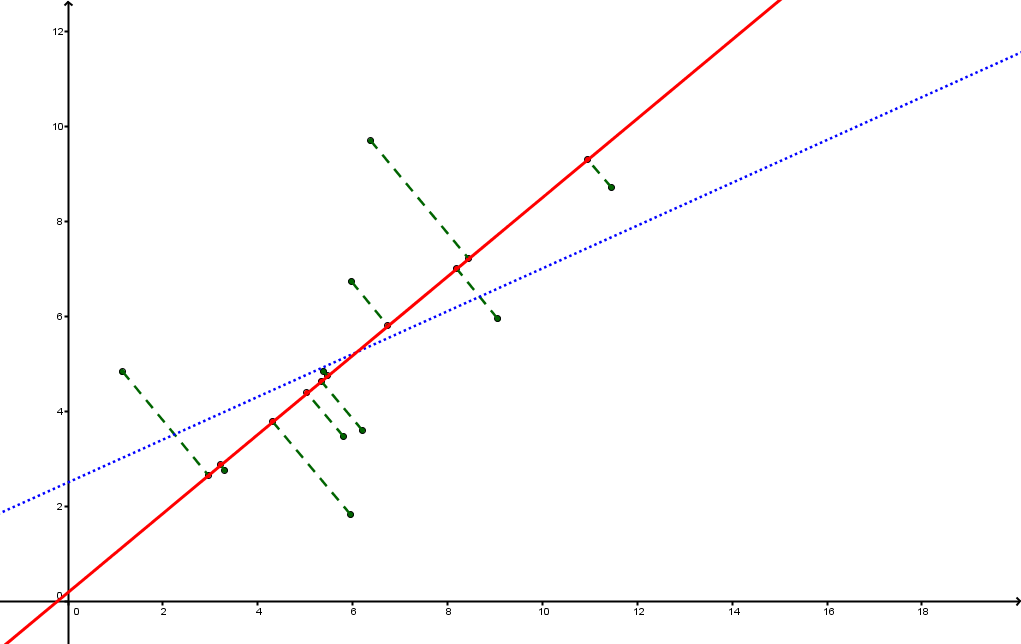
\includegraphics[width=11cm]{../fig/Cap10-Regresion-MAR.png}
\end{enColor}
\begin{bn}
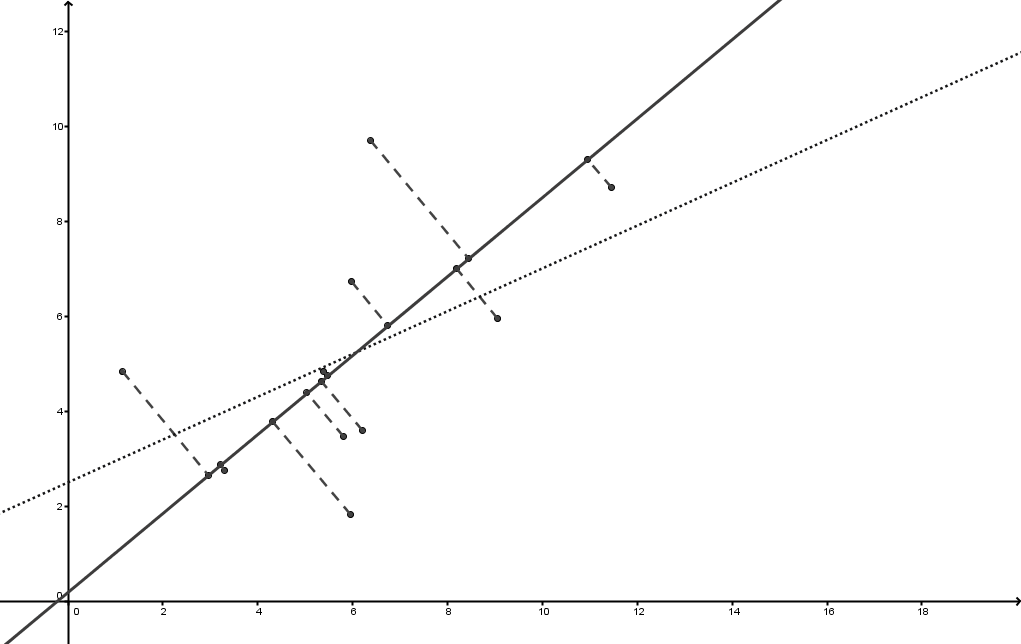
\includegraphics[width=11cm]{../fig/Cap10-Regresion-MAR-bn.png}
\end{bn}
\caption{Recta de regresión ortogonal (major axis, en trazo continuo) y recta de regresión por mínimos cuadrados (trazo a puntos), para el mismo conjunto de puntos.}
\label{cap10:fig:RegresionMAR}
\end{center}
\end{figure}

La recta de regresión por el método de mínimos cuadrados (que es la recta de la que hemos hablado hasta ahora en el Capítulo) se muestra en trazo a puntos y en color azul. La recta que se obtiene por el método de regresión ortogonal (major axis) se muestra en trazo continuo y color rojo.  Además, para esta segunda recta se indican los segmentos  que conectan cada punto $(x_i,y_i)$ de la muestra con el correspondiente punto predicho $(\hat x_i, \hat y_i)$ sobre la recta. Como puede verse, lo que caracteriza a este método de regresión es que esos segmentos son perpendiculares a la recta. Compáralos con los segmentos que van de cada punto al punto predicho en la Figura \ref{cap10:fig:InterpretacionErrorCuadratico} (pág. \pageref{cap10:fig:InterpretacionErrorCuadratico}). Aquellos eran verticales.
\qed
\end{ejemplo}
Aunque en este curso no vamos a entrar a fondo en el tema de la regresión ortogonal y otros esquemas alternativos de regresión, en el Tutorial10 daremos unas breves instrucciones sobre la forma de obtener la recta de regresión usando regresión ortogonal.

¿Cuál de las dos rectas es ``mejor''? La respuesta es, naturalmente, que depende de lo que deseemos obtener. Y, además, hay que tener en cuenta que cuando una de las rectas produce una aproximación muy buena a los puntos $(x_i, y_i)$, la otra también lo hace. Porque, en esos casos, las dos rectas se parecen mucho. Eso, entre otras cosas, explica porque en muchos cursos de introducción a la Estadística ni siquiera se menciona que existen otros tipos de regresión. Y es una lástima, porque hay varias razones que hacen que la regresión ortogonal sea muy interesante:
\begin{itemize}
  \item En primer lugar, queremos destacar que la regresión ortogonal, a diferencia de la regresión por mínimos cuadrados, no depende de los ejes de coordenadas. Gráficamente puedes pensar en lo que sucede si, manteniendo las posiciones relativas de los puntos $(x_i, y_i)$, borramos los ejes de coordenadas y giramos el plano de coordenadas. ¿Cuál sería entonces la recta más adecuada? La de la regresión ortogonal.
  \item En particular, eso hace que el método de regresión ortogonal se puede considerar un primer paso hacia la técnica de Análisis de Componentes Principales, que es una herramienta básica en cursos más avanzados de Estadística. Daremos alguna referencia adicional sobre esto en el Apéndice \ref{apendice:MasAlla}.

  \item Además, en el Capítulo \ref{cap:RegresionLogistica}, cuando hablemos de modelos lineales generalizados, el hecho de conocer dos modelos de regresión nos va a ayudar a comprender que el modelo no puede considerarse completo hasta que no se entiende la estructura de error que lo conforma. Retomaremos entonces esta discusión.
      %Todavía es demasiado pronto para que el lector pueda entender bien de qué se trata. Pero  es importante observar, lo antes posible, que el objetivo en la regresión por mínimos cuadrados es minimizar la suma de las áreas de los cuadrados

\end{itemize}
Otra posible razón por la que muchos textos obvian la existencia de la regresión ortogonal es que las fórmulas que se deben utilizar en este método son más complicadas que las que corresponden al método de mínimos cuadrados.

La regresión por mínimos cuadrados y la regresión ortogonal no agotan, como hemos dicho, el catálogo de posibilidades a la hora de aproximar los puntos $(x_i, y_i)$ por una recta. Por ejemplo, en lugar de movernos en vertical para llegar a la recta (como se hace en el método de mínimos cuadrados), podríamos movernos en horizontal. Esto tiene pleno sentido cuando lo que se busca es predecir los valores de $x$ a partir de valores {\sf fijos} de la variable $y$. La recta que se obtiene al hacer esto es, en general, distinta de la de mínimos cuadrados. Una posibilidad, entonces es hacer ambas rectas, y calcular su bisectriz, cuya pendiente es, en algún sentido, un promedio de las pendientes de esas dos rectas. E incluso hay otra forma de promediar las pendientes de estas dos rectas, calculando su media geométrica. Este segundo método se conoce, en inglés, como {\em reduced major axis regression (RMA)}\index{reduced mayor axis regression}\index{regression, reduced major axis}\index{RMA, reduced mayor axis regression}. En español no hay una terminología universalmente aceptada. Es importante entender que esta recta, obtenida usando RMA, es una recta distinta de las que se obtienen usando mínimos cuadrados o usando regresión ortogonal.

Como se ve, la respuesta a ``¿cuál es la mejor recta?'' es algo más complicada de lo que parecía.



\section{Análisis de la varianza. Coeficiente $r$ de correlación lineal de Pearson.}
\label{cap10:sec:AnovaCoeficienteCorrelacion}


Ya hemos aprendido que no debemos extrapolar. Pero, recordando de nuevo las preguntas que hemos dejado pendientes desde el comienzo de la Sección \ref{cap10:subsec:ComoElegirLaMejorRecta} (pág. \pageref{cap10:subsec:ComoElegirLaMejorRecta}), está claro que esto, al fin y al cabo, nos dice cómo {\em no debemos} usar la recta. Pero todavía no sabemos medir cómo de buena es la recta cuando la usamos correctamente, sin extrapolar. Es decir, cuando la usamos para predecir valores que no forman parte de la muestra (pero siempre con valores de $x$ dentro del recorrido de la muestra). Para eso, como ya sabemos, tenemos que dejar la tranquilidad de la Estadística Descriptiva (al fin y al cabo la recta de regresión es una {\em descripción} de la muestra), y adentrarnos en el siempre más complicado territorio de la Inferencia. Pero en esta sección, antes de hacer eso, vamos a usar, por primera vez en el curso, una técnica estadística muy valiosa, llamada Análisis de la Varianza. Esta técnica es más conocida por la abreviatura de su nombre en inglés. De {\em ANalysis Of VAriance} obtenemos Anova. Es el método más usado para estudiar la relación entre varias variables, y veremos en detalle su versión más conocida en el Capítulo \ref{cap:IntroduccionAnova}. El Anova nos servirá después de guía en la Inferencia basada en la regresión, que veremos en la siguiente sección.

Para llegar hasta ahí, vamos a abordar ahora la pregunta de cómo podemos medir la calidad de la recta que hemos obtenido. Es muy importante entender, para empezar,  esto: dado un conjunto de $n$ puntos del plano
\[(x_1,y_1),\ldots,(x_n,y_n)\]
con dos o más puntos, y que no estén todos ellos en una misma recta vertical, {\em la recta de regresión siempre se puede calcular}. Si repasas las fórmulas, verás que lo único que se necesita, para poder calcular esa recta, es que sea $s^2(x)\neq 0$, y para eso basta con las condiciones que hemos impuesto.

Pero poder calcular algo no quiere decir que sea útil hacerlo. Hay conjuntos de puntos para los que esa recta, incluso siendo la mejor de las rectas que podemos elegir, es bastante mala. Para darte una idea de las diversas razones por las que eso puede suceder, te ofrecemos dos ejemplos (veremos los cálculos necesarios en el Tutorial 10).

\begin{ejemplo}\label{cap10:ejem:RectaMalaAproximacion01}
En el ejemplo que se muestra en la Figura \ref{cap10:fig:EjemploRectaMalaAproximacion01}(a) puedes ver que el conjunto de $30$ puntos con el que empezamos:
{\small
\begin{center}
\begin{tabular}{llllll}
    $(0.463, 0.25)$, &  $(0.952, 0.043)$,&  $(0.785, 0.17)$,&  $(0.764, 0.18)$,& $(0.726, 0.2)$,\\
    $(0.913, 0.079)$,&  $(0.799, 0.16)$, & $(0.934, 0.062)$,& $(0.82, 0.15)$,  & $(0.00456, 0.005)$,\\  $(0.247, 0.19)$,& $(0.754, 0.19)$,   & $(0.858, 0.12)$, & $(0.624, 0.24)$, &$(0.715, 0.2)$,\\
    $(0.978, 0.02)$,& $(0.941, 0.055)$,  & $(0.0773, 0.072)$,& $(0.33, 0.22)$, & $(0.55, 0.25)$,\\
    $(0.0451, 0.043)$,&  $(0.0745, 0.067)$,&  $(0.81, 0.15)$,& $(0.271, 0.2)$, & $(0.463, 0.25)$,\\  $(0.156, 0.13)$,&  $(0.673, 0.22)$, &  $(0.459, 0.25)$,  & $(0.252, 0.19)$,& $(0.81, 0.15)$.
\end{tabular}
\end{center}
}
%{\small
%$
%(0.463, 0.25)$, $(0.952, 0.043)$, $(0.785, 0.17)$, $(0.764, 0.18)$, $(0.252, 0.19)$, $(0.726, 0.2)$, $(0.913, 0.079)$, $(0.799, 0.16)$, $(0.934, 0.062)$, $(0.82, 0.15)$, $(0.00456, 0.005)$, $(0.247, 0.19)$, $(0.754, 0.19)$, $(0.858, 0.12)$, $(0.624, 0.24)$, $(0.715, 0.2)$, $(0.978, 0.02)$, $(0.941, 0.055)$, $(0.0773, 0.072)$, $(0.33, 0.22)$, $(0.55, 0.25)$, $(0.0451, 0.043)$, $(0.0745, 0.067)$, $(0.81, 0.15)$, $(0.271, 0.2)$, $(0.463, 0.25)$, $(0.156, 0.13)$, $(0.673, 0.22)$, $(0.81, 0.15)$, $(0.459, 0.25)$
%}\\[3mm]
 se sitúa muy aproximadamente a lo largo de una parábola (concretamente $y=x-x^2$). Y, desde luego, podemos calcular la correspondiente recta de regresión, que resulta ser \[y=0.1529-0.004669\cdot x\]
que se representa, junto con los puntos, en la Figura \ref{cap10:fig:EjemploRectaMalaAproximacion01}(b). Como puede verse, la recta es muy poco representativa de ese conjunto de puntos. En la Figura \ref{cap10:fig:EjemploRectaMalaAproximacion01}(c) hemos añadido la parábola, para que quede clara la diferencia.

Por cierto, como referencia para más adelante, la covarianza en este ejemplo es:
\[\Cov(x,y)\approx -0.0004560\]

\begin{figure}[p]
\begin{center}
\begin{enColor}
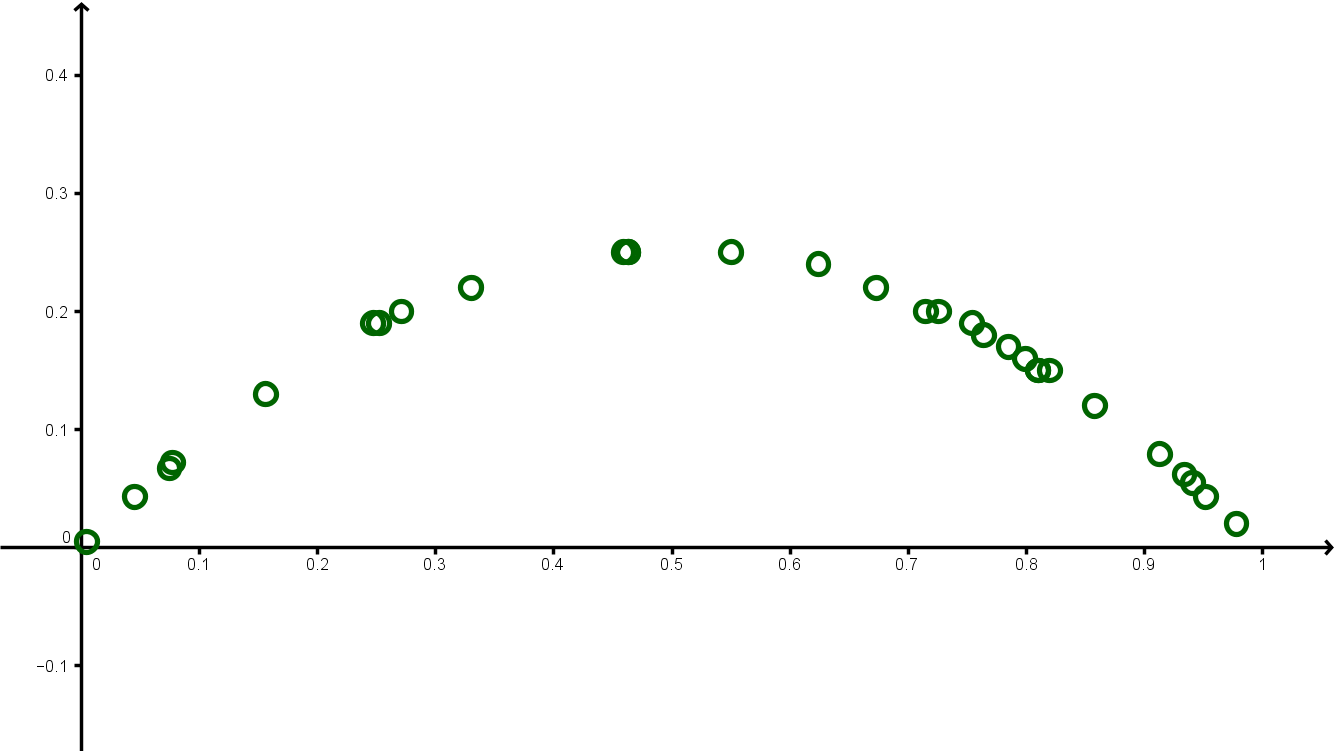
\includegraphics[height=6cm]{../fig/Cap10-EjemploRectaMalaAproximacion01a.png}\\
(a) El punto de partida es este conjunto de puntos (diagrama de dispersi\'on).\\
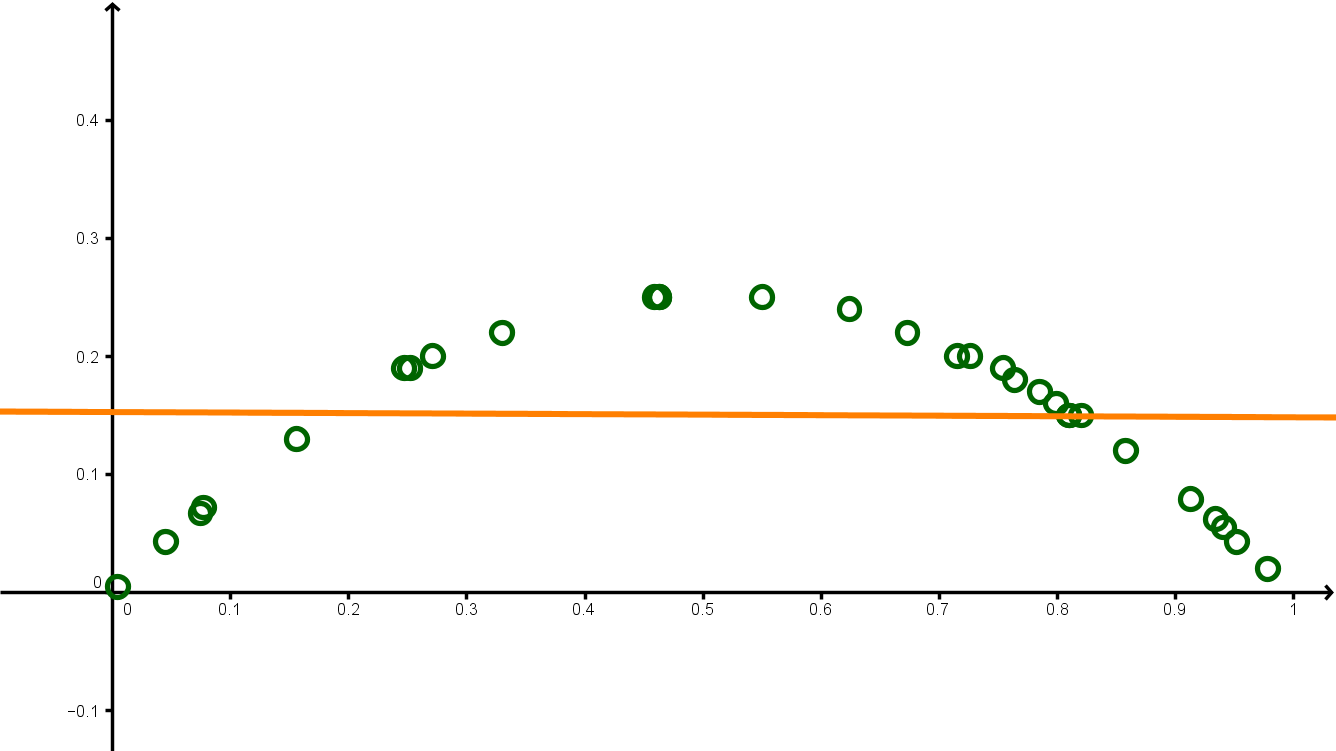
\includegraphics[height=6cm]{../fig/Cap10-EjemploRectaMalaAproximacion01b.png}\\
(b) Y podemos ajustar una recta de regresi\'on de muy mala calidad...
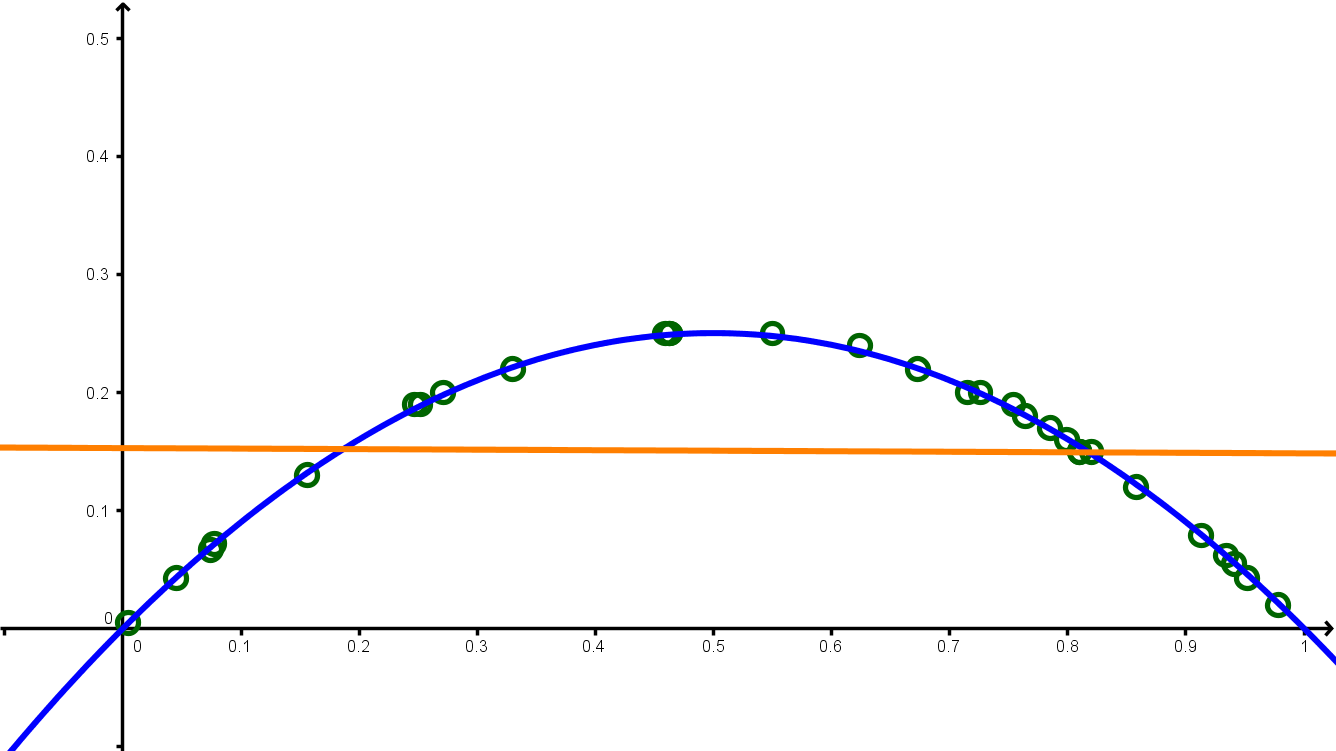
\includegraphics[height=6cm]{../fig/Cap10-EjemploRectaMalaAproximacion01c.png}\\
(c) ... pero los puntos est\'an pidiendo a gritos que les ajustemos una par\'abola.
\end{enColor}
\begin{bn}
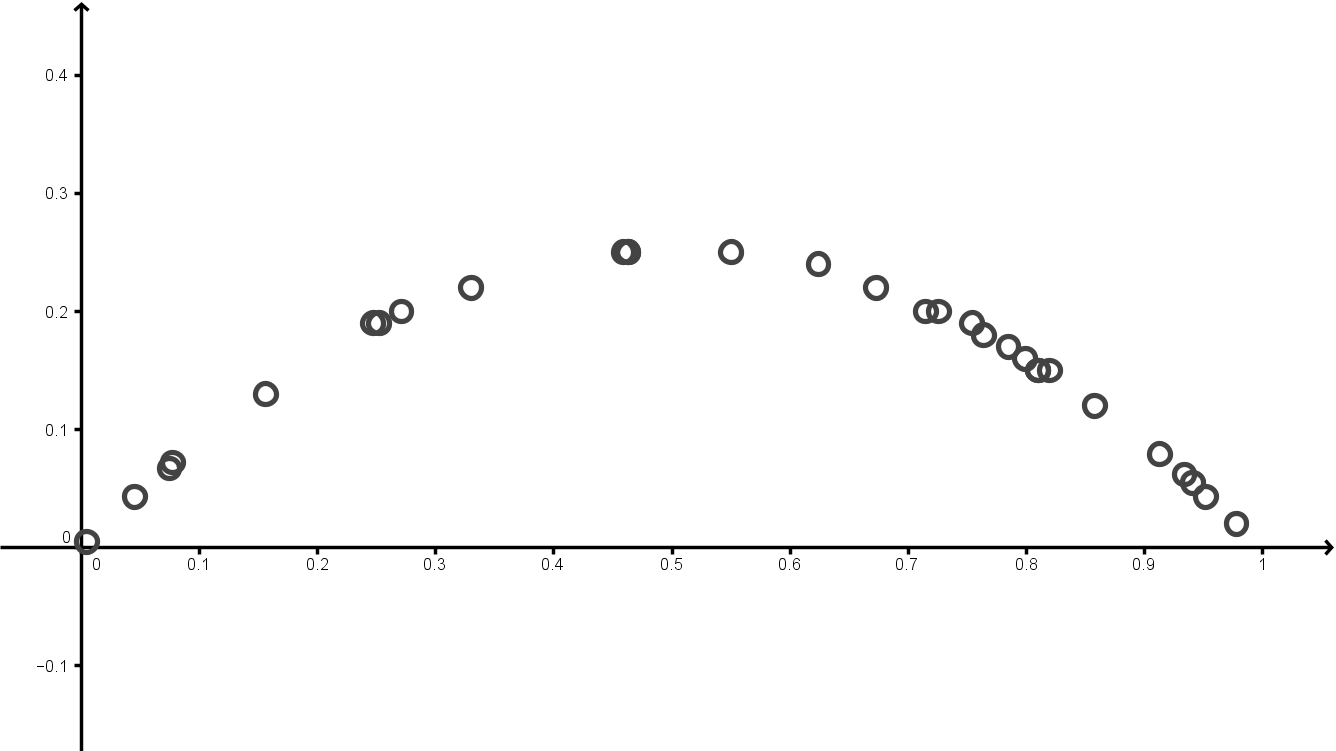
\includegraphics[height=6cm]{../fig/Cap10-EjemploRectaMalaAproximacion01a-bn.png}\\
(a) El punto de partida es este conjunto de puntos (diagrama de dispersi\'on).\\
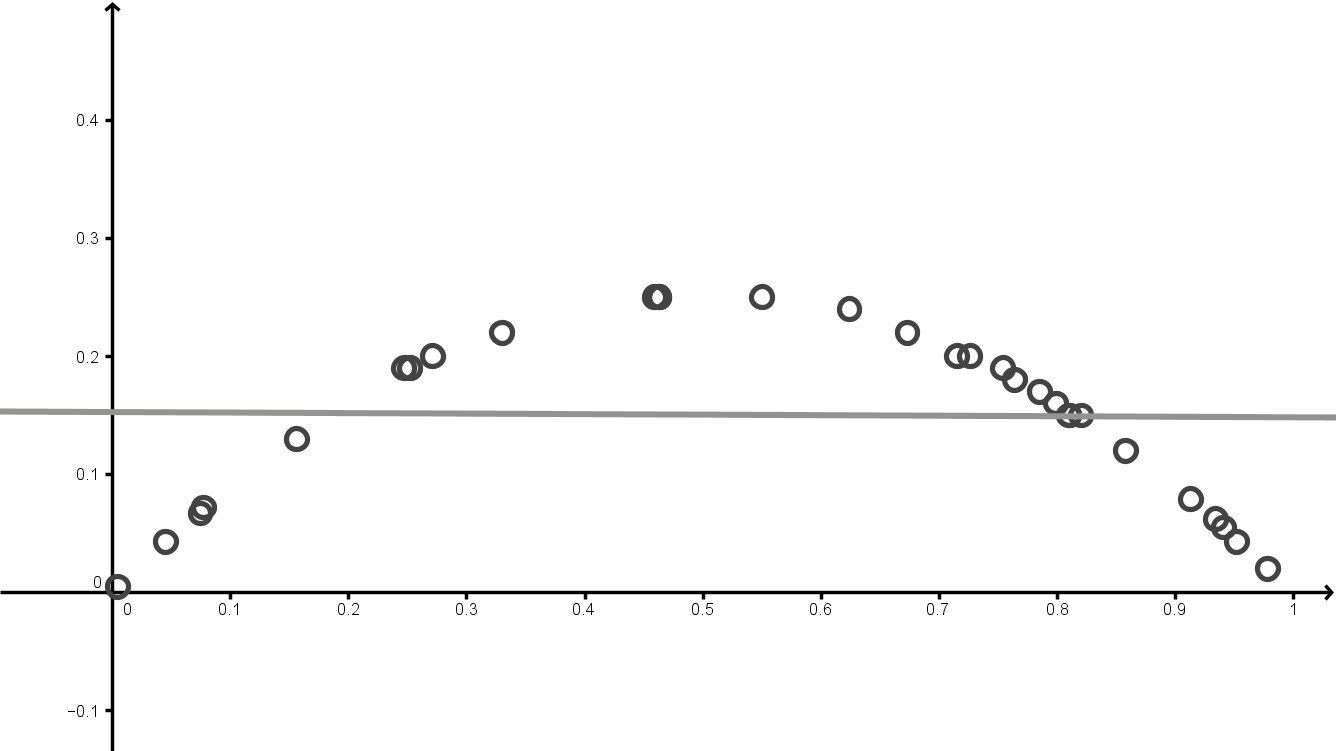
\includegraphics[height=6cm]{../fig/Cap10-EjemploRectaMalaAproximacion01b-bn.png}\\
(b) Y podemos ajustar una recta de regresi\'on de muy mala calidad...
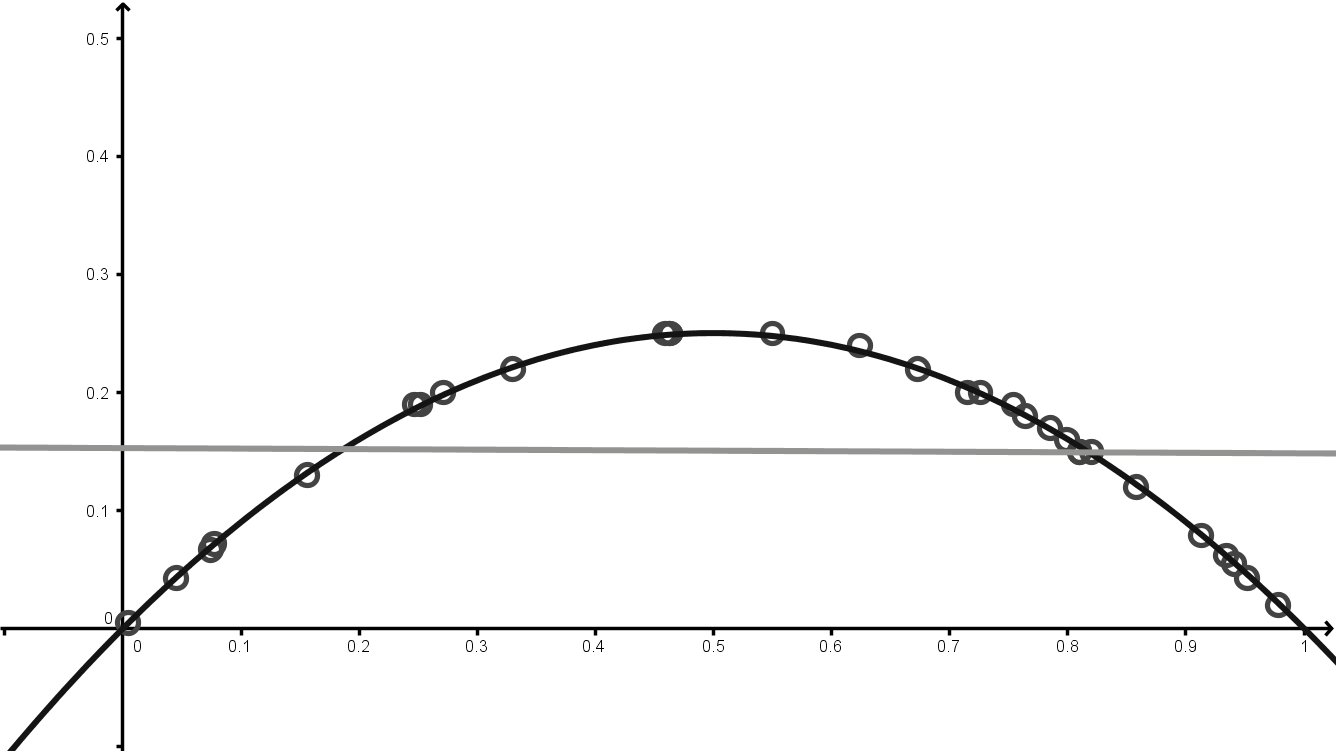
\includegraphics[height=6cm]{../fig/Cap10-EjemploRectaMalaAproximacion01c-bn.png}\\
(c) ... pero los puntos est\'an pidiendo a gritos que les ajustemos una par\'abola.
\end{bn}
\caption{Un ejemplo de recta de regresión de muy mala calidad.}
\label{cap10:fig:EjemploRectaMalaAproximacion01}
\end{center}
\end{figure}

\qed
\end{ejemplo}

Este ejemplo nos deja, además, algunos interrogantes adicionales: si hay una curva, como la parábola de este ejemplo, que hace el trabajo mejor que la recta, ¿cómo podemos saberlo, y cómo podemos encontrar cuál es esa parábola? Volveremos sobre esto más adelante.

El siguiente ejemplo ilustra un fenómeno distinto.
\begin{ejemplo}\label{cap10:ejem:RectaMalaAproximacion02}
En la Figura \ref{cap10:fig:EjemploRectaMalaAproximacion02} (pág. \pageref{cap10:fig:EjemploRectaMalaAproximacion02}) puedes ver este otro conjunto de $30$ puntos:\\
{\small
\begin{center}
\begin{tabular}{lllll}
$(0.987,0.973)$,&  $(0.666,0.207)$,&  $(0.463,0.502)$,&  $(0.107,0.799)$,&  $(0.715,0.0619)$, \\
$(0.612,0.364)$,&  $(0.33,0.282)$,&  $(0.479,0.0189)$,&  $(0.852,0.373)$,&  $(0.424,0.0225)$, \\
$(0.615,0.269)$,&  $(0.75,0.262)$,&  $(0.455,0.482)$,&  $(0.917,0.644)$,&  $(0.853,0.114)$, \\
$(0.722,0.0421)$,&  $(0.76,0.5)$,&  $(0.625,0.838)$,&  $(0.704,0.12)$,&  $(0.49,0.00395)$, \\
$(0.0677,0.484)$,&  $(0.137,0.737)$,&  $(0.205,0.176)$,&  $(0.643,0.879)$,&  $(0.203,0.182)$,\\
$(0.89,0.722)$,&  $(0.0577,0.0964)$,&  $(0.101,0.874)$,&  $(0.953,0.742)$,&  $(0.104,0.567)$
\end{tabular}
\end{center}
}
que se encuentra muy repartido en todo el cuadrado definido por las desigualdades simultáneas $0\leq x\leq 1$, $0\leq y\leq 1$. En este caso, también es posible calcular una recta de regresión, que se muestra en esa figura, y resulta ser
\[y=0.4272+0.02296\cdot x,\]
pero de nuevo vemos que esa recta no sirve para gran cosa como representante del conjunto de puntos. En este caso, la pregunta es más bien ¿por qué estamos tratando de encontrar una relación de la forma $y=f(x)$, cuando la figura sugiere que los valores de $x$ y los de $y$ son esencialmente independientes?

Y de nuevo, como referencia, la covarianza en este ejemplo vale:
\[\Cov(x,y)\approx -0.002242\]

\begin{figure}[ht]
\begin{center}
\begin{enColor}
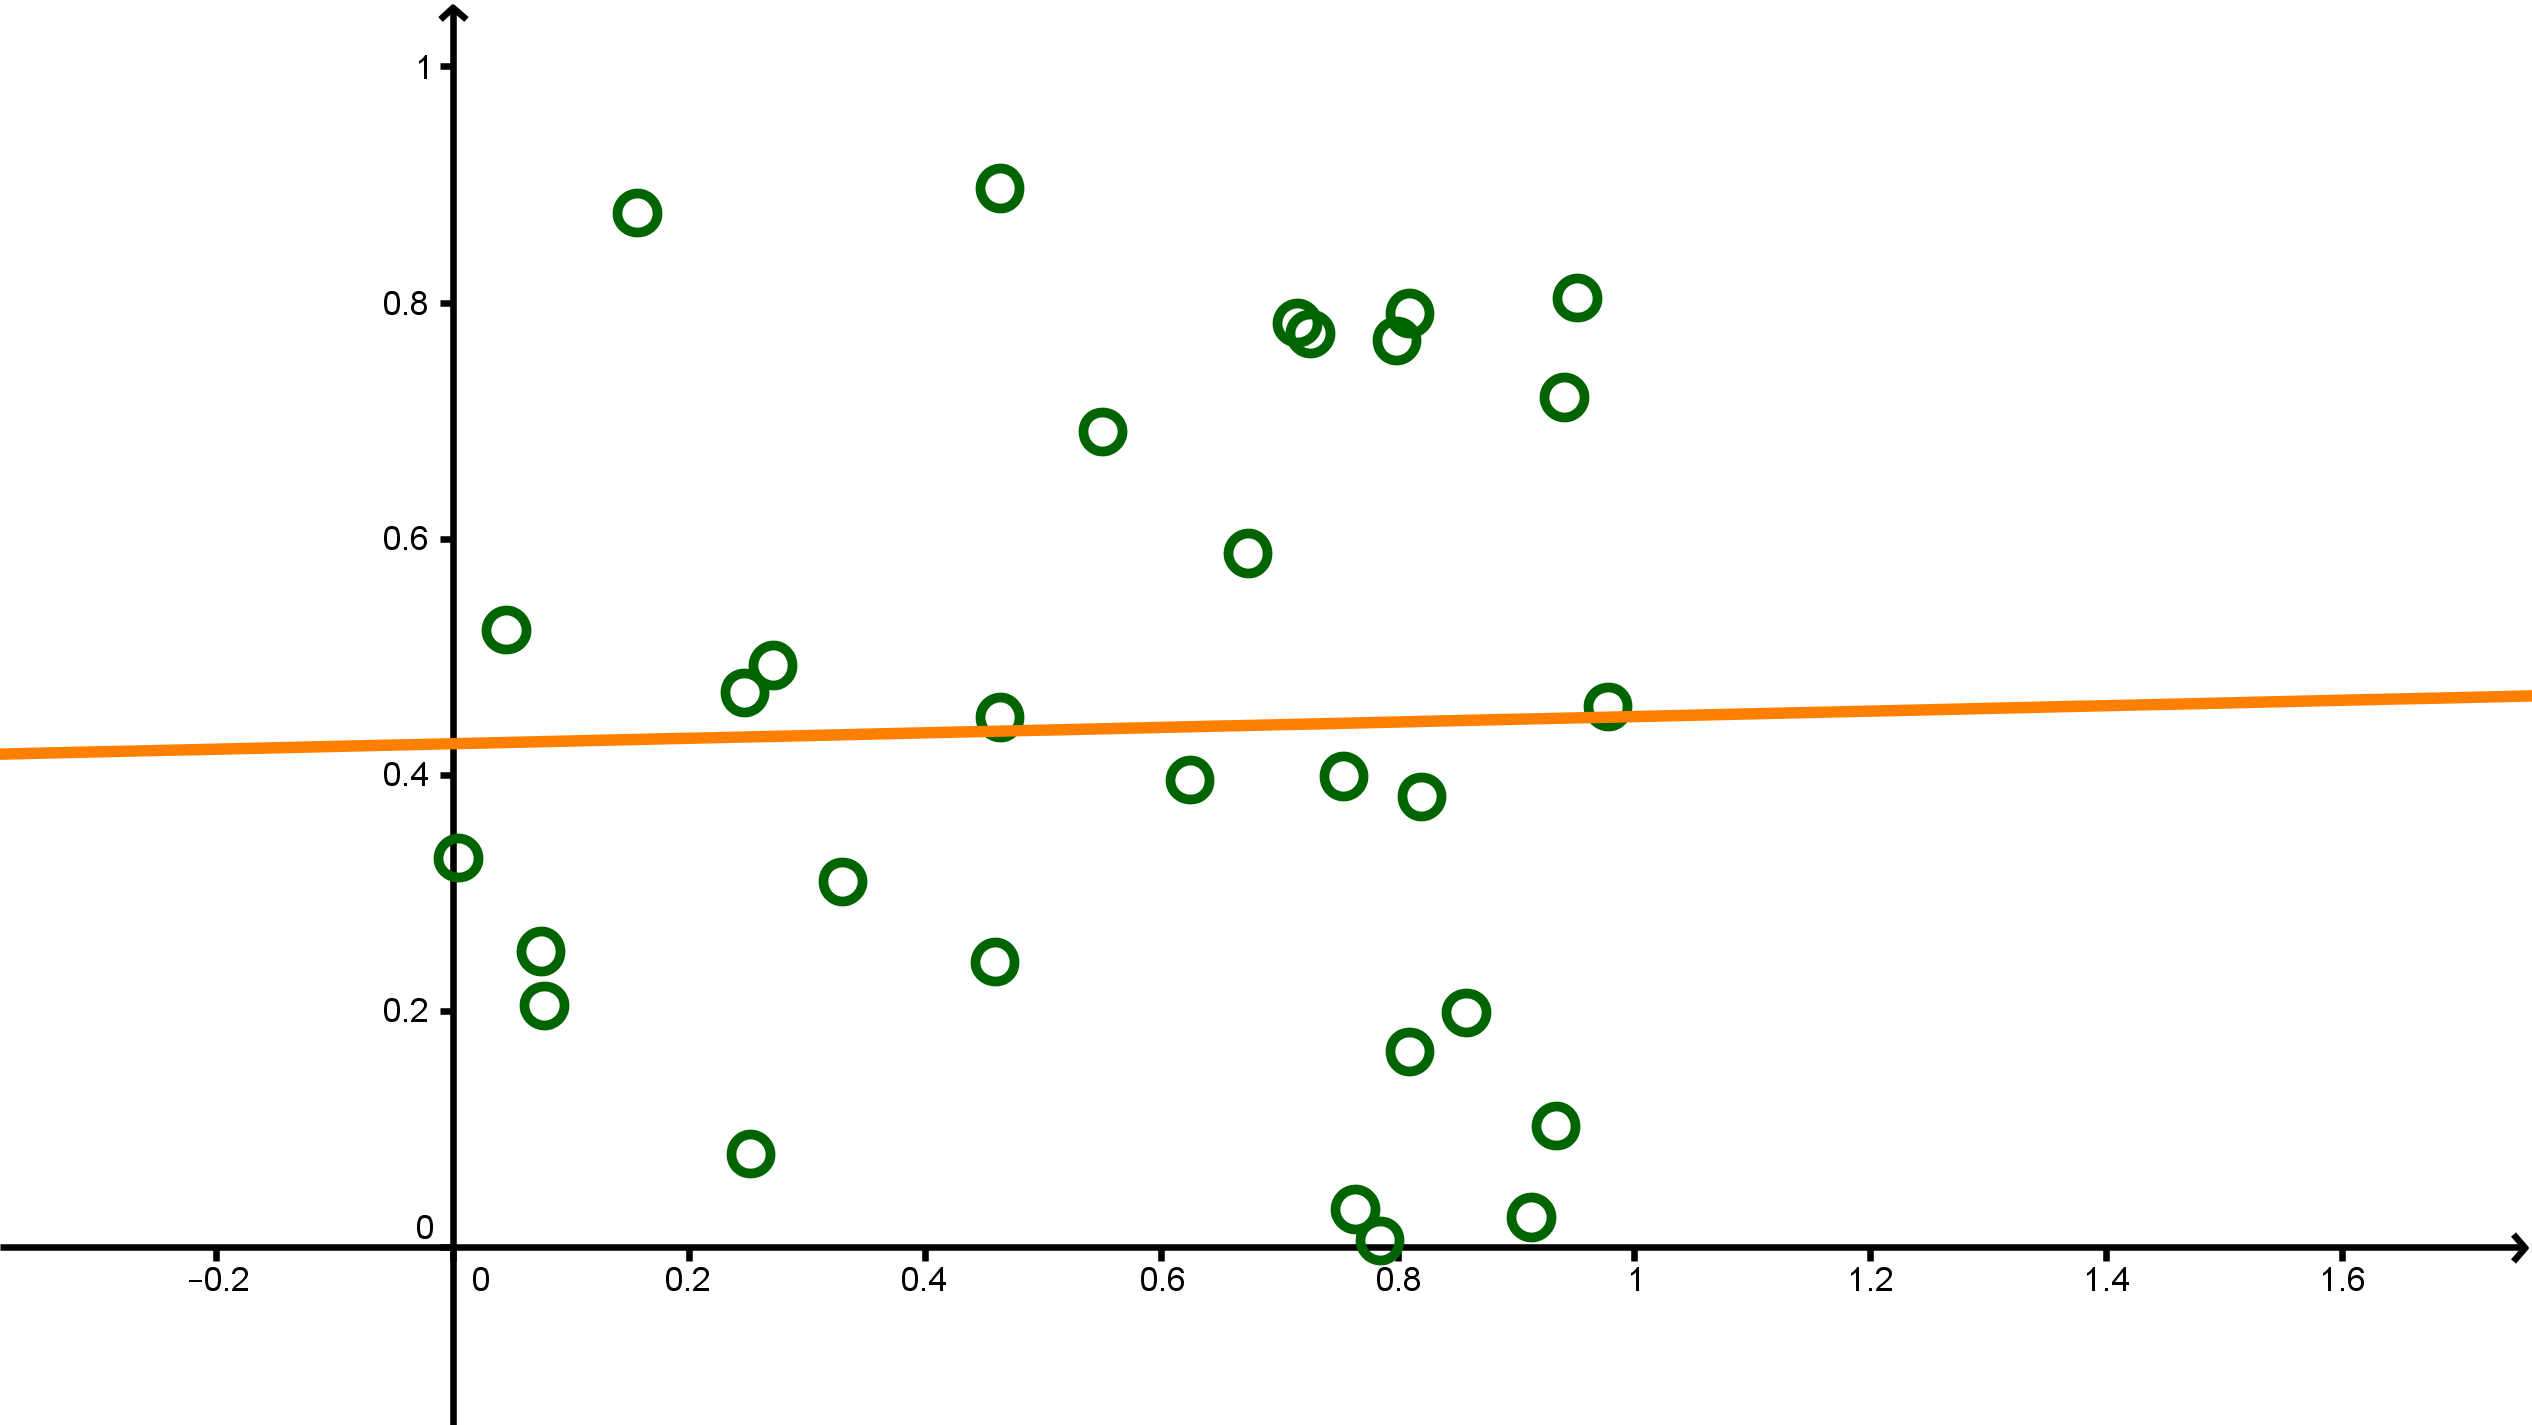
\includegraphics[height=6cm]{../fig/Cap10-EjemploRectaMalaAproximacion02.png}
\end{enColor}
\begin{bn}
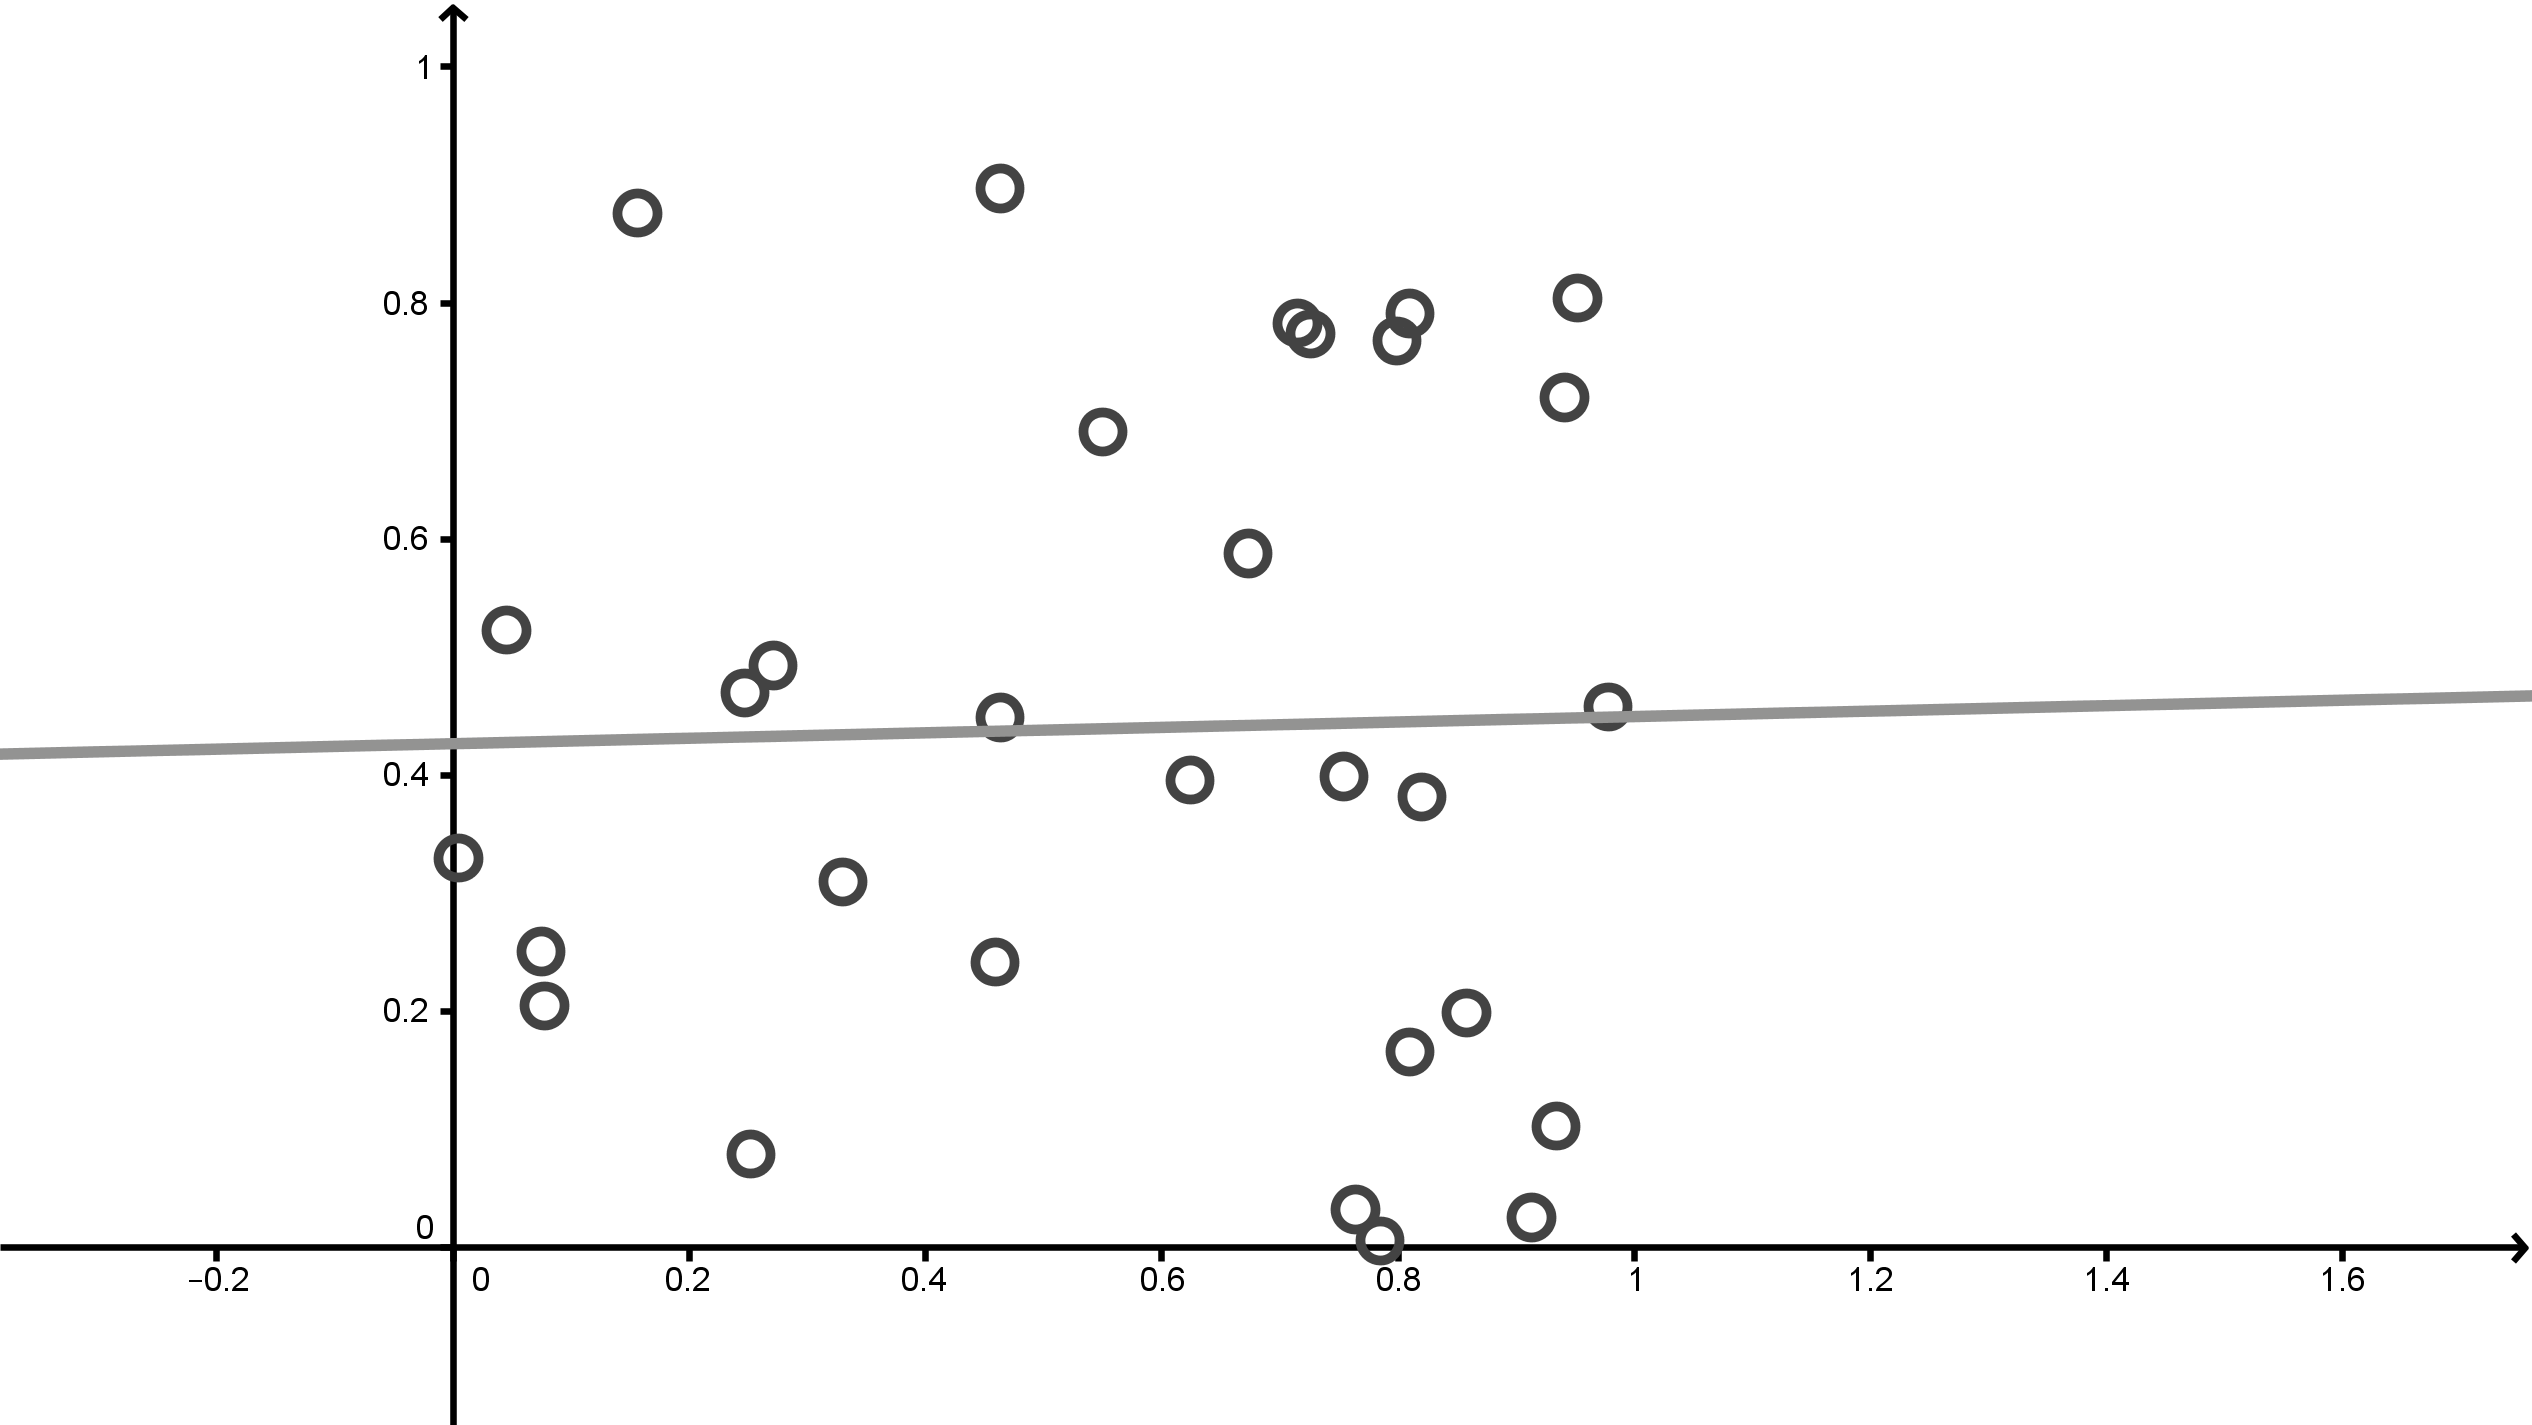
\includegraphics[height=6cm]{../fig/Cap10-EjemploRectaMalaAproximacion02-bn.png}
\end{bn}
\caption{Otra razón por la que la recta de regresión puede ser de muy mala calidad.}
\label{cap10:fig:EjemploRectaMalaAproximacion02}
\end{center}
\end{figure}

\qed
\end{ejemplo}


A la vista de estos ejemplos, está claro que tenemos que preguntarnos: ¿cómo podemos estar seguros de que el ajuste de la recta a los datos es de buena calidad?

Un punto de partida razonable parece ser pensar sobre el error cuadrático EC que hemos usado para definir la recta (ver la Ecuación \ref{cap10:ecu:ErrorCuadratico}, pág. \pageref{cap10:ecu:ErrorCuadratico}).
\[\mbox{EC}(y=b_0+b_1\cdot x)=\sum_{i=1}^n(y_i-\hat y_i)^2 = \sum_{i=1}^n(y_i-b_0-b_1\cdot x_i)^2.\]
Al fin y al cabo, la idea original era que si ese error es pequeño, la recta sería buena...
Y una vez más nos tropezamos con una dificultad que ya hemos encontrado en situaciones parecidas. Es un problema de escala: ¿pequeño, comparado con qué? El tamaño absoluto del EC depende de las
unidades de medida que se estén utilizando, y por eso es difícil usarlo directamente como
un indicador fiable de calidad. Queremos obtener un indicador de calidad que no dependa
de la escala del problema. Para conseguir eso vamos a hacer un análisis más detallado del error cuadrático.

\subsection{Identidad Anova.}
\label{cap10:subsec:identidadAnova}

Recordemos que el objetivo básico es medir la diferencia entre los valores iniciales de
la coordenada $y$:
\[y_1, y_2,\ldots, y_n,\]
y los valores que predice la recta de regresión:
\[\hat y_1,\hat y_2,\ldots,\hat y_n,\]
Además, tenemos la media $\bar y$ de los valores iniciales. Con esta media podemos calcular
la cuasivarianza de $y$:
\[s^2(y)=\dfrac{1}{n-1}\sum_{i=1}^{n}(y_i-\bar y)^2\]
y al ver esta fórmula, nos damos cuenta de que el sumatorio que aparece en ella recuerda bastante al EC:
\[\mbox{EC}(y=b_0+b_1\cdot x)=\sum_{i=1}^n(y_i-\hat y_i)^2\]
De hecho, al compararlas está claro que podemos escribir un tercer sumatorio, en el que
relacionamos la media con los valores que predice la regresión:
\[\sum_{i=1}^n(\hat y_i-\bar y)^2\]
Con este tercer ingrediente, estamos en condiciones de hacer una descomposición o {\sf Análisis de la
Varianza}\index{análisis de la Varianza}\index{Anova}(Anova) de $y$. Se puede demostrar (no es
difícil) que siempre se cumple esta identidad:
    \begin{center}
    \fcolorbox{black}{Gris025}{
    \begin{minipage}{7.5cm}
    \begin{equation}\label{cap10:ecu:AnovaparaRegresion}
    \displaystyle\sum_{i=1}^{n}(y_i-\bar y)^2 =
    \mbox{EC}+\sum_{i=1}^n(\hat y_i-\bar y)^2
    \end{equation}
       %%%%%%%%%%%%%%%%%%%%%%%%%%%%%%%%%%%%%%%
    \end{minipage}
    }
    \end{center}
Para entender lo que significa esta descomposición es necesario pensar un poco en el significado del error cuadrático EC. Conviene recordar la discusión que hicimos en torno a la Figura \ref{cap10:fig:ErrorCuadraticoIgual0} (pág. \pageref{cap10:fig:ErrorCuadraticoIgual0}). El error cuadrático {\em sólo puede ser $0$ cuando los puntos $(x_i,y_i)$ están alineados, y es tanto más grande cuanto menos alineados estén.} En concreto, si los puntos estuvieran perfectamente alineados (y por tanto $y_i=\hat y_i$), la identidad \ref{cap10:ecu:AnovaparaRegresion} se convertiría en:
\[
\displaystyle\sum_{i=1}^{n}(y_i-\bar y)^2 =
    0 + \sum_{i=1}^n(\hat y_i-\bar y)^2.
\]
El primer término de esta identidad representa siempre, en todos los casos, la {\sf dispersión total} de los valores $y_i$ respecto de la media $\bar y$. Y la observación que hemos hecho es que, si los puntos están alineados, la dispersión total viene dada por el último término:
\[\sum_{i=1}^n(\hat y_i-\bar y)^2\]
Así que es posible interpretar este término como {\em la parte de la variación total de $y$ que se explica mediante la recta de regresión}.

Vamos a tratar de aclarar lo que queremos decir con esto. En el caso más habitual en las aplicaciones, como el ejemplo del {\em Herrerillo} con el que hemos abierto este capítulo, los valores $y_i$ están relacionados con los $x_i$, mediante una relación de la forma
\[y=b_0+b_1\cdot x,\]
pero esa relación es {\em ruidosa}, por la presencia de muchos otros factores aleatorios que introducen alteraciones en los valores que observamos. Pero, incluso si los valores $y_i$ se calcularan usando la fórmula,
\[y=b_0+b_1\cdot x\]
{\em sin introducir ningún ruido aleatorio}, incluso en ese caso seguirían teniendo un cierto grado de dispersión, simplemente por el hecho de que no son iguales entre sí. Veamos un ejemplo detallado para ilustrar la identidad \ref{cap10:ecu:AnovaparaRegresion} y el Anova basado en ella.

\begin{ejemplo}
\label{cap10:ejem:Anova01}
Empecemos con los valores $x_1,\ldots,x_{10}$ de esta lista
\[0.25, 0.46, 0.73, 0.76, 0.78, 0.8, 0.82, 0.91, 0.93, 0.95.\]
En primer lugar, usaremos la recta $y=1-\dfrac{x}{2}$ para fabricar 10 valores de la variable $y$, {\sf sin introducir ningún ruido aleatorio en el proceso}. Los puntos $(x_i,y_i)$ que se obtienen son los que se muestran en la  Tabla \ref{cap10:tabla:Anova01noruidosos} (en el Tutorial10 podrás comprobar estos cálculos usando el ordenador).
\begin{table}[htb]
\centering
\begin{tabular}{rrrrrrrrrrr}
  \hline
$i$ & 1 & 2 & 3 & 4 & 5 & 6 & 7 & 8 & 9 & 10 \\
  \hline
$x_i$ & 0.25 & 0.46 & 0.73 & 0.76 & 0.78 & 0.80 & 0.82 & 0.91 & 0.93 & 0.95 \\
$y_i$ & 0.88 & 0.77 & 0.64 & 0.62 & 0.61 & 0.60 & 0.59 & 0.54 & 0.53 & 0.52 \\
   \hline
\end{tabular}
\caption{Puntos ``no ruidosos'' del Ejemplo \ref{cap10:ejem:Anova01}}
\label{cap10:tabla:Anova01noruidosos}
\end{table}
En la Figura \ref{cap10:fig:Anova01} se muestran los puntos $(x_i,y_i)$ y su proyección sobre el eje $y$. Podemos calcular la media y la dispersión total de los valores $y_1,\ldots,y_{10}$:
\[\bar y\approx 0.6305, \qquad \displaystyle\sum_{i=1}^{n}(y_i-\bar y)^2=(n-1)\cdot s^2(y)\approx 0.1099\]
Y lo más importante de este ejemplo es darse cuenta de que la dispersión de los $y_i$, reflejada por ese valor de $s^2(y)$, se debe {\sf completamente} a que la recta los produce, y al hacerlo  refleja en ellos la dispersión de los puntos $x_i$ de partida. Por así decirlo, en este ejemplo, el azar se acaba una vez que se han generado los puntos $x_i$. A partir de ahí, la recta fabrica los valores $y_i$, sin que intervenga nada aleatorio en ese paso. Por eso decimos que la dispersión $(n-1)\cdot s^2(y)$, en este caso, es dispersión explicada completamente por la recta. En números, el último término de la identidad \ref{cap10:ecu:AnovaparaRegresion} es:
\[\sum_{i=1}^n(\hat y_i-\bar y)^2=\sum_{i=1}^n\left((1-\dfrac{x_i}{2})-0.6305\right)^2,\]
y sustituyendo los valores de los $x_i$, obtenemos, como era de esperar, el mismo valor que al calcular $(n-1)\cdot s^2(y)$:
\[\sum_{i=1}^n(\hat y_i-\bar y)^2\approx 0.1099\]

\begin{figure}[p]
\begin{center}
\begin{enColor}
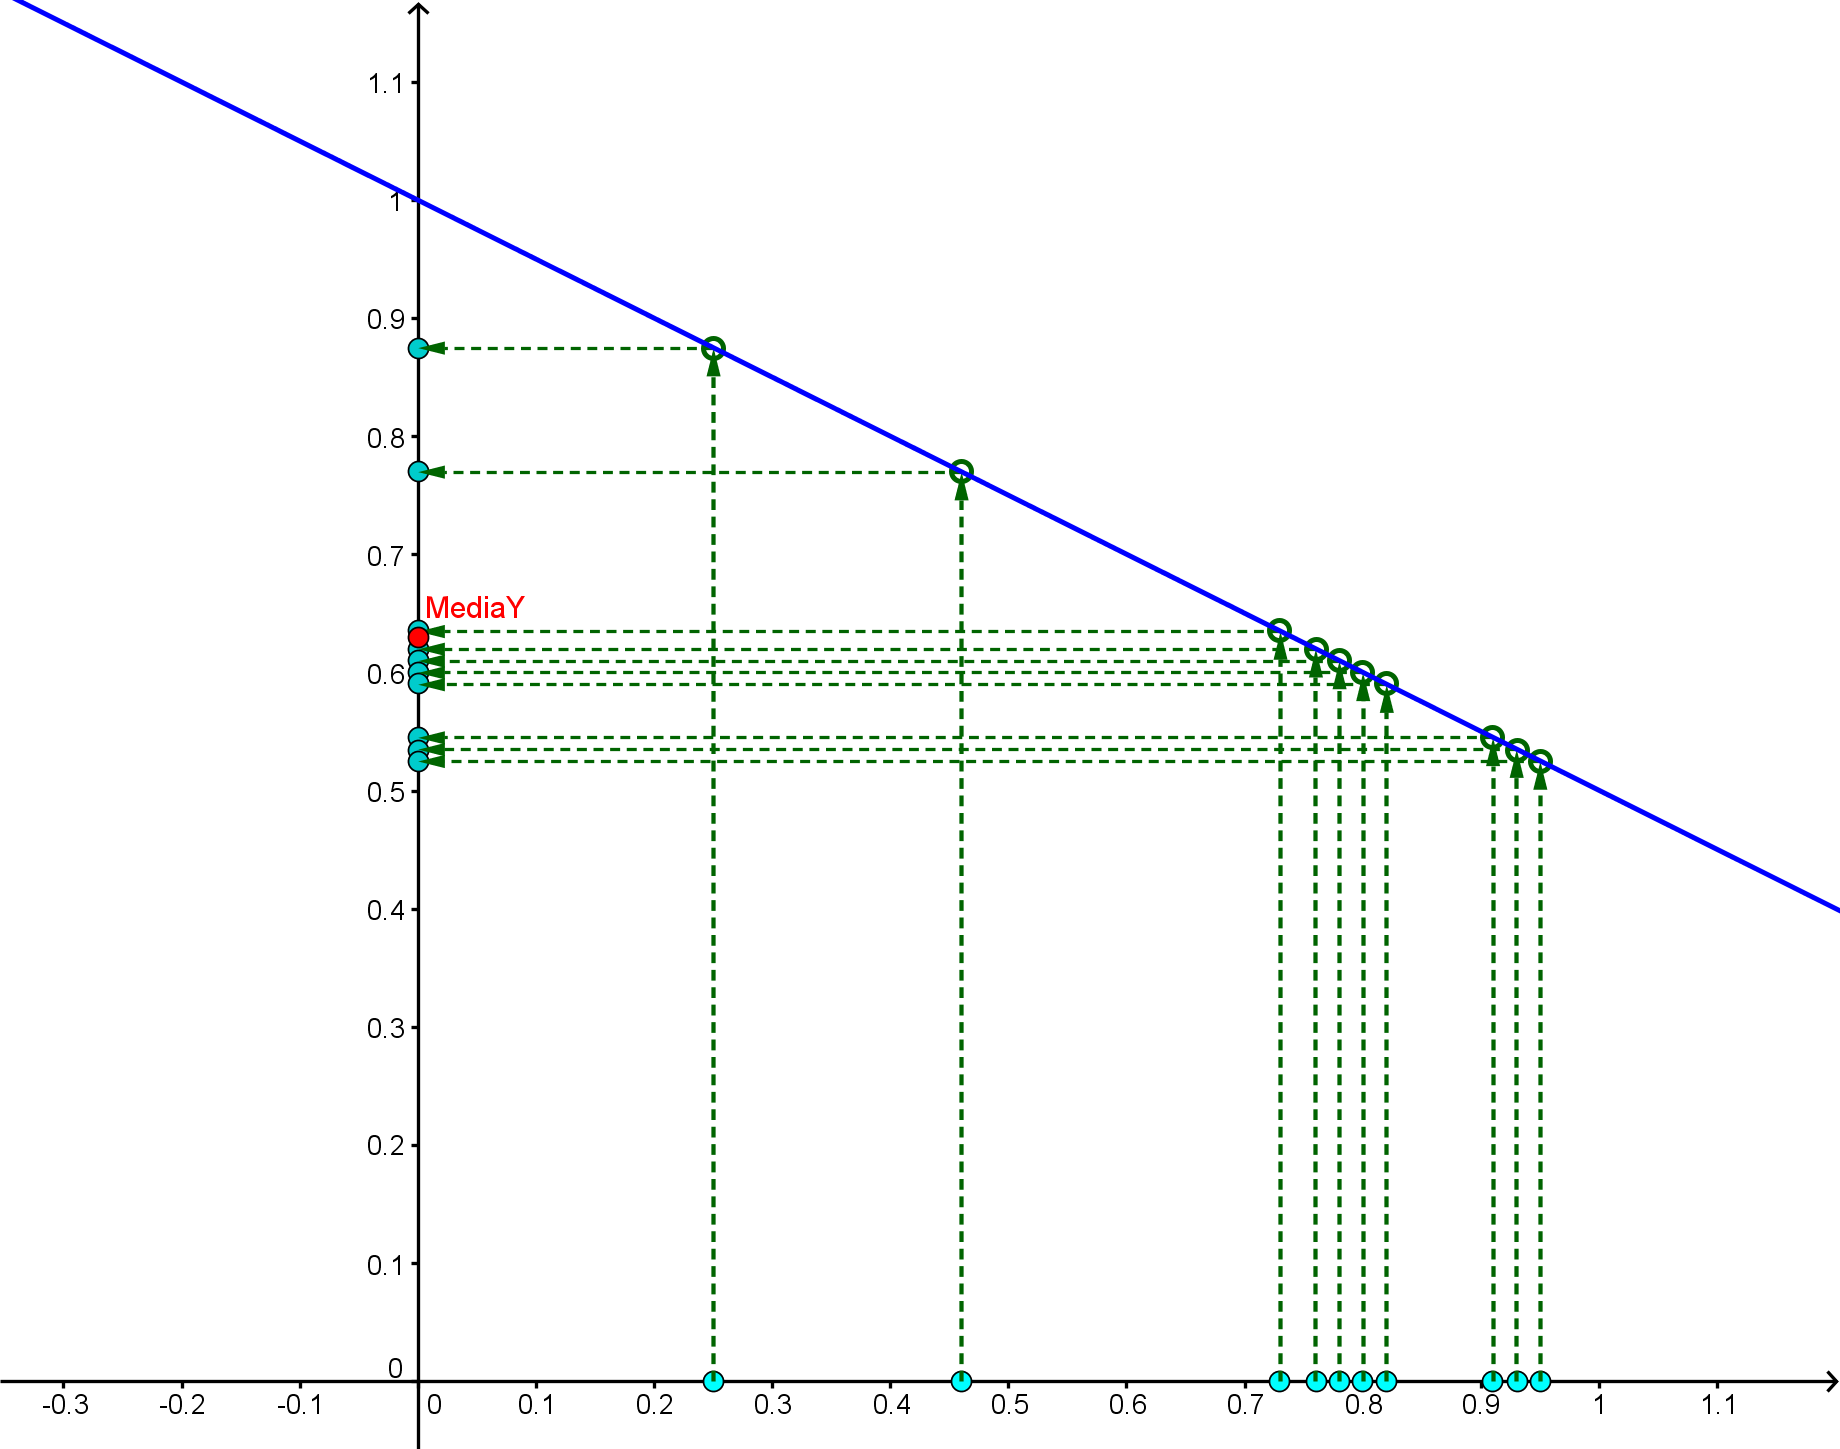
\includegraphics[height=10cm]{../fig/Cap10-Anova01.png}
\end{enColor}
\begin{bn}
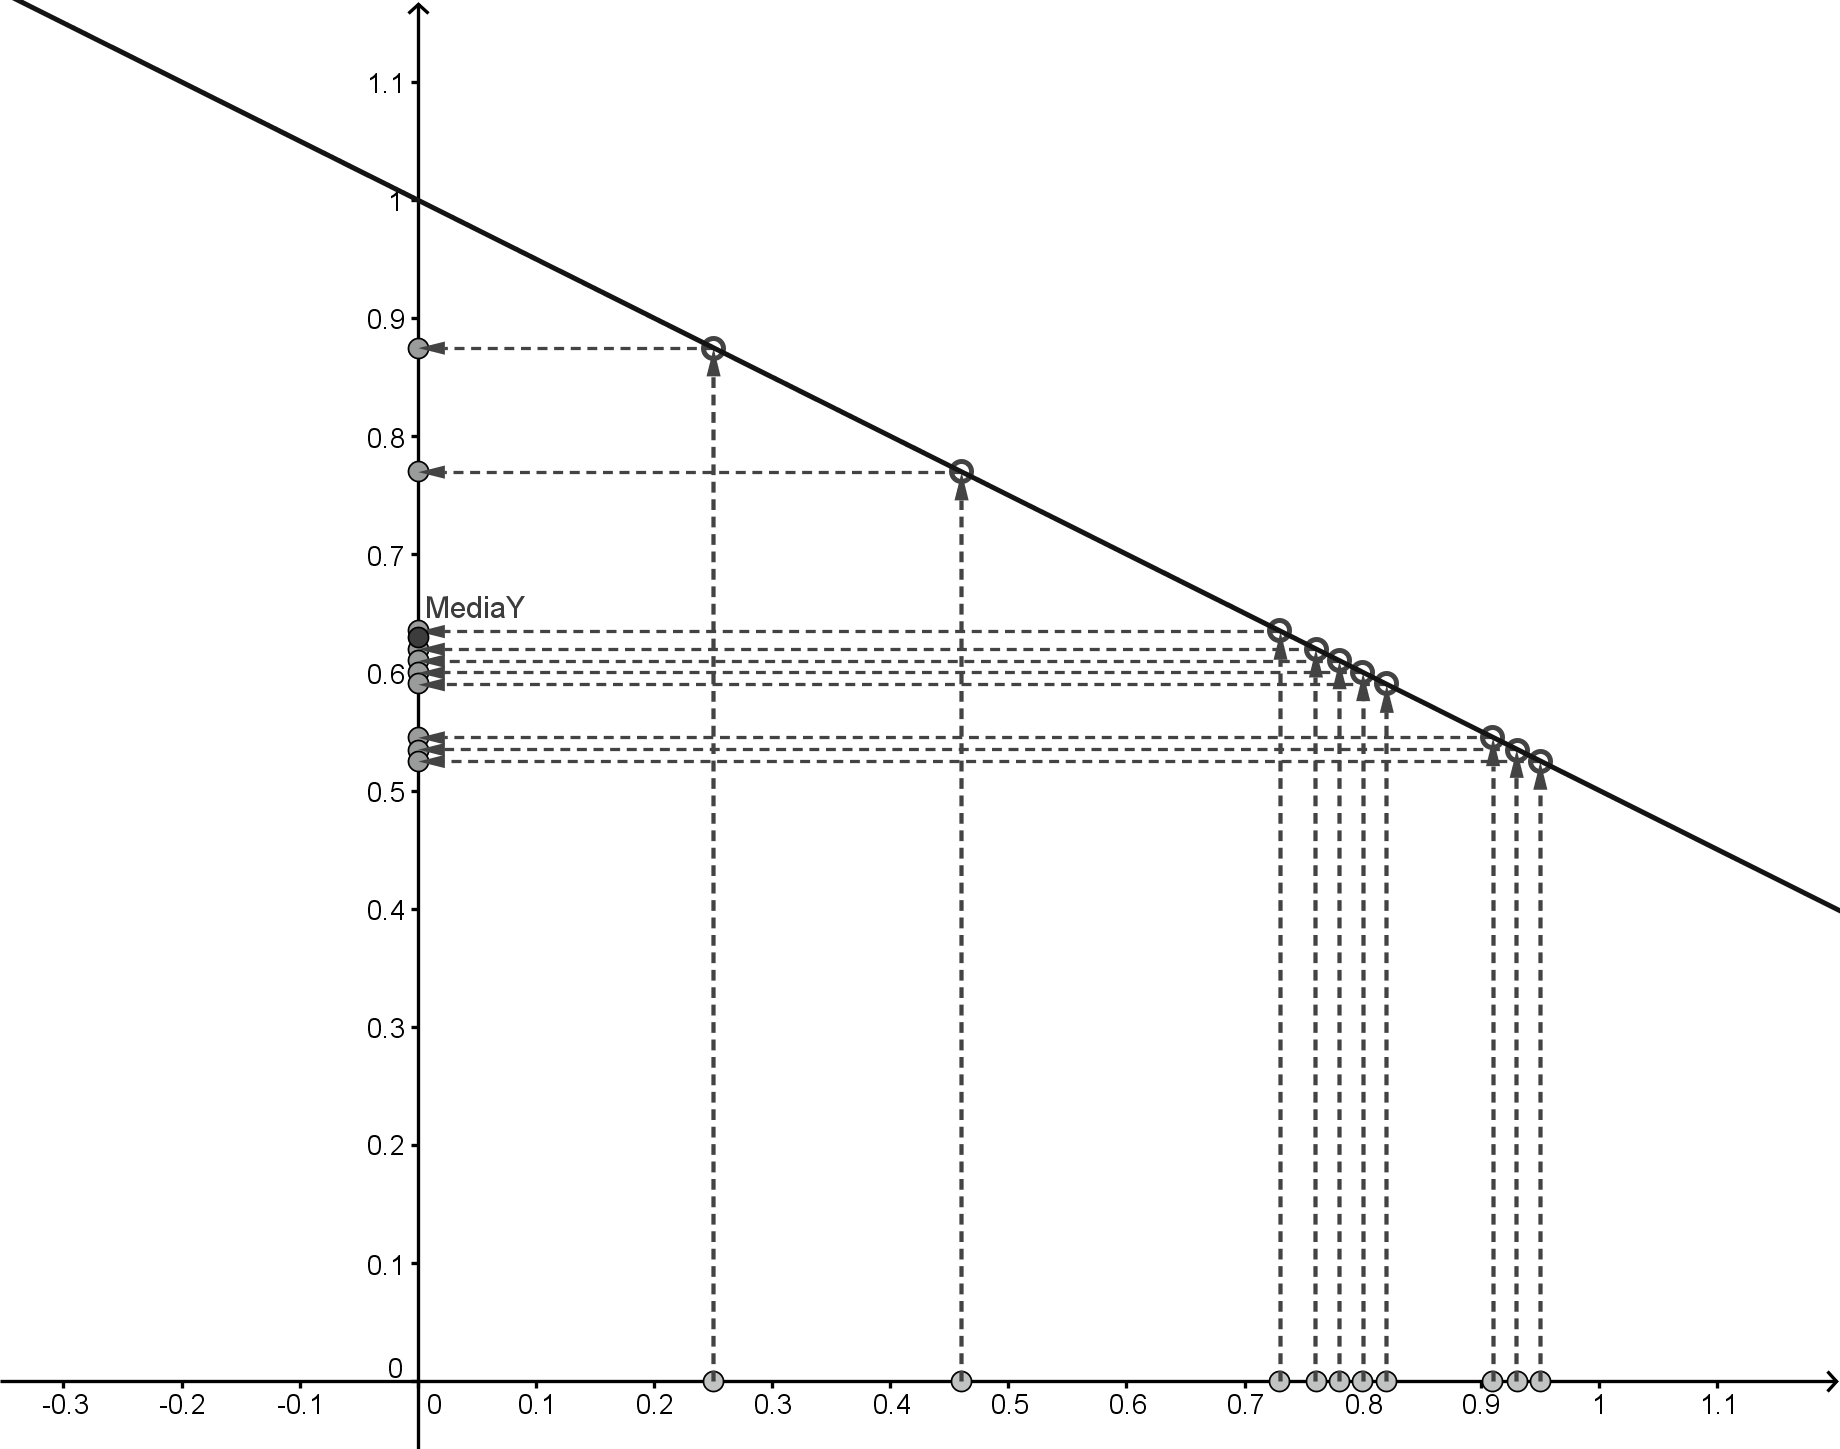
\includegraphics[height=10cm]{../fig/Cap10-Anova01-bn.png}
\end{bn}
\caption{Anova en la regresión. Caso ``no ruidoso'',  en el que la dispersión de los valores $y_i$ se explica completamente por el efecto de la recta.}
\label{cap10:fig:Anova01}
\end{center}
\end{figure}

\begin{figure}[p]
\begin{center}
\begin{enColor}
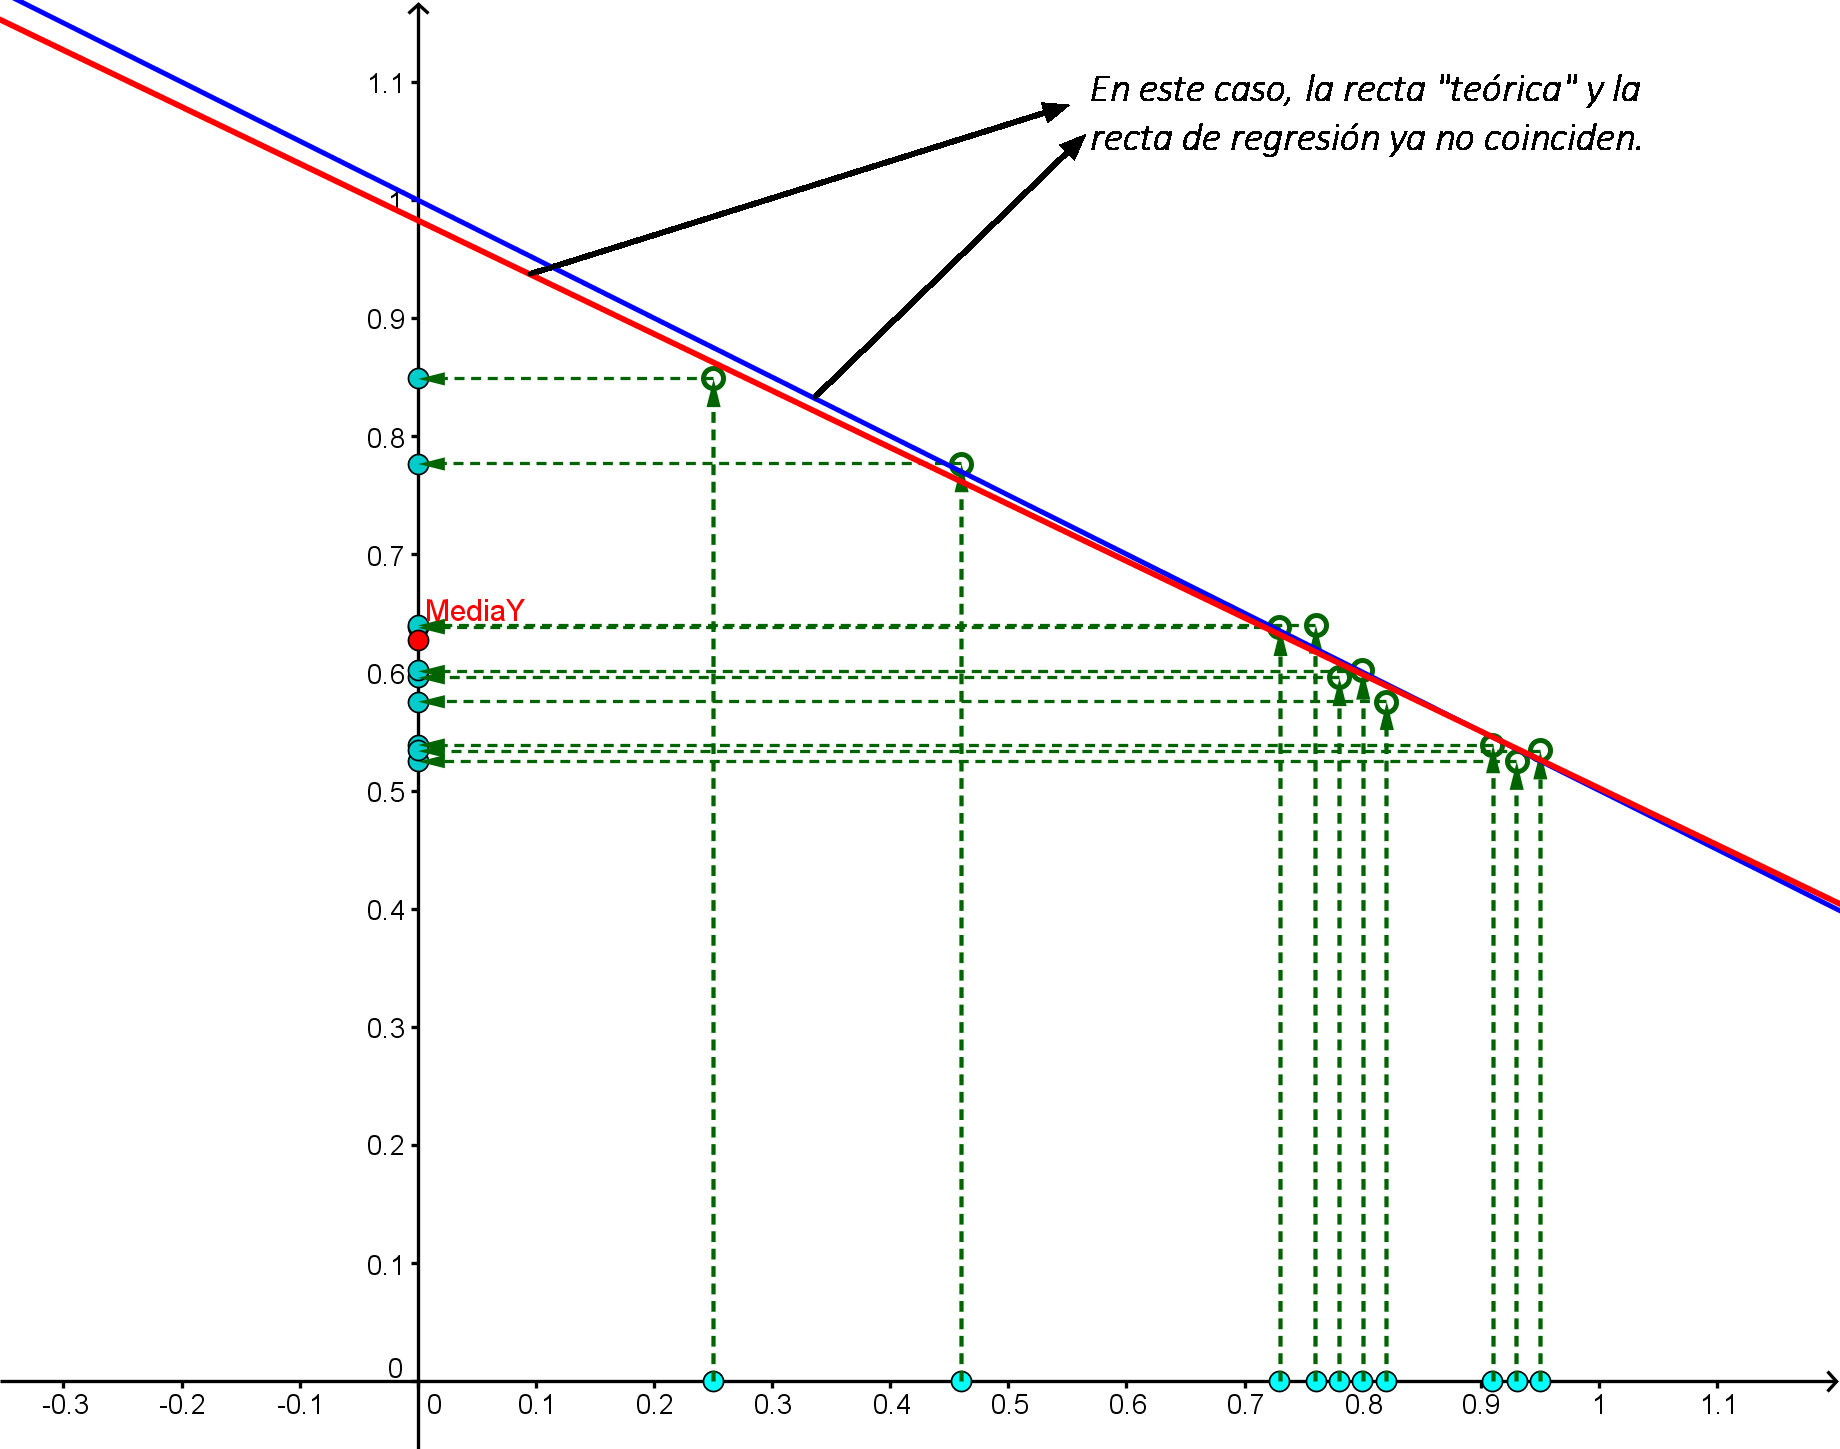
\includegraphics[height=10cm]{../fig/Cap10-Anova02.png}
\end{enColor}
\begin{bn}
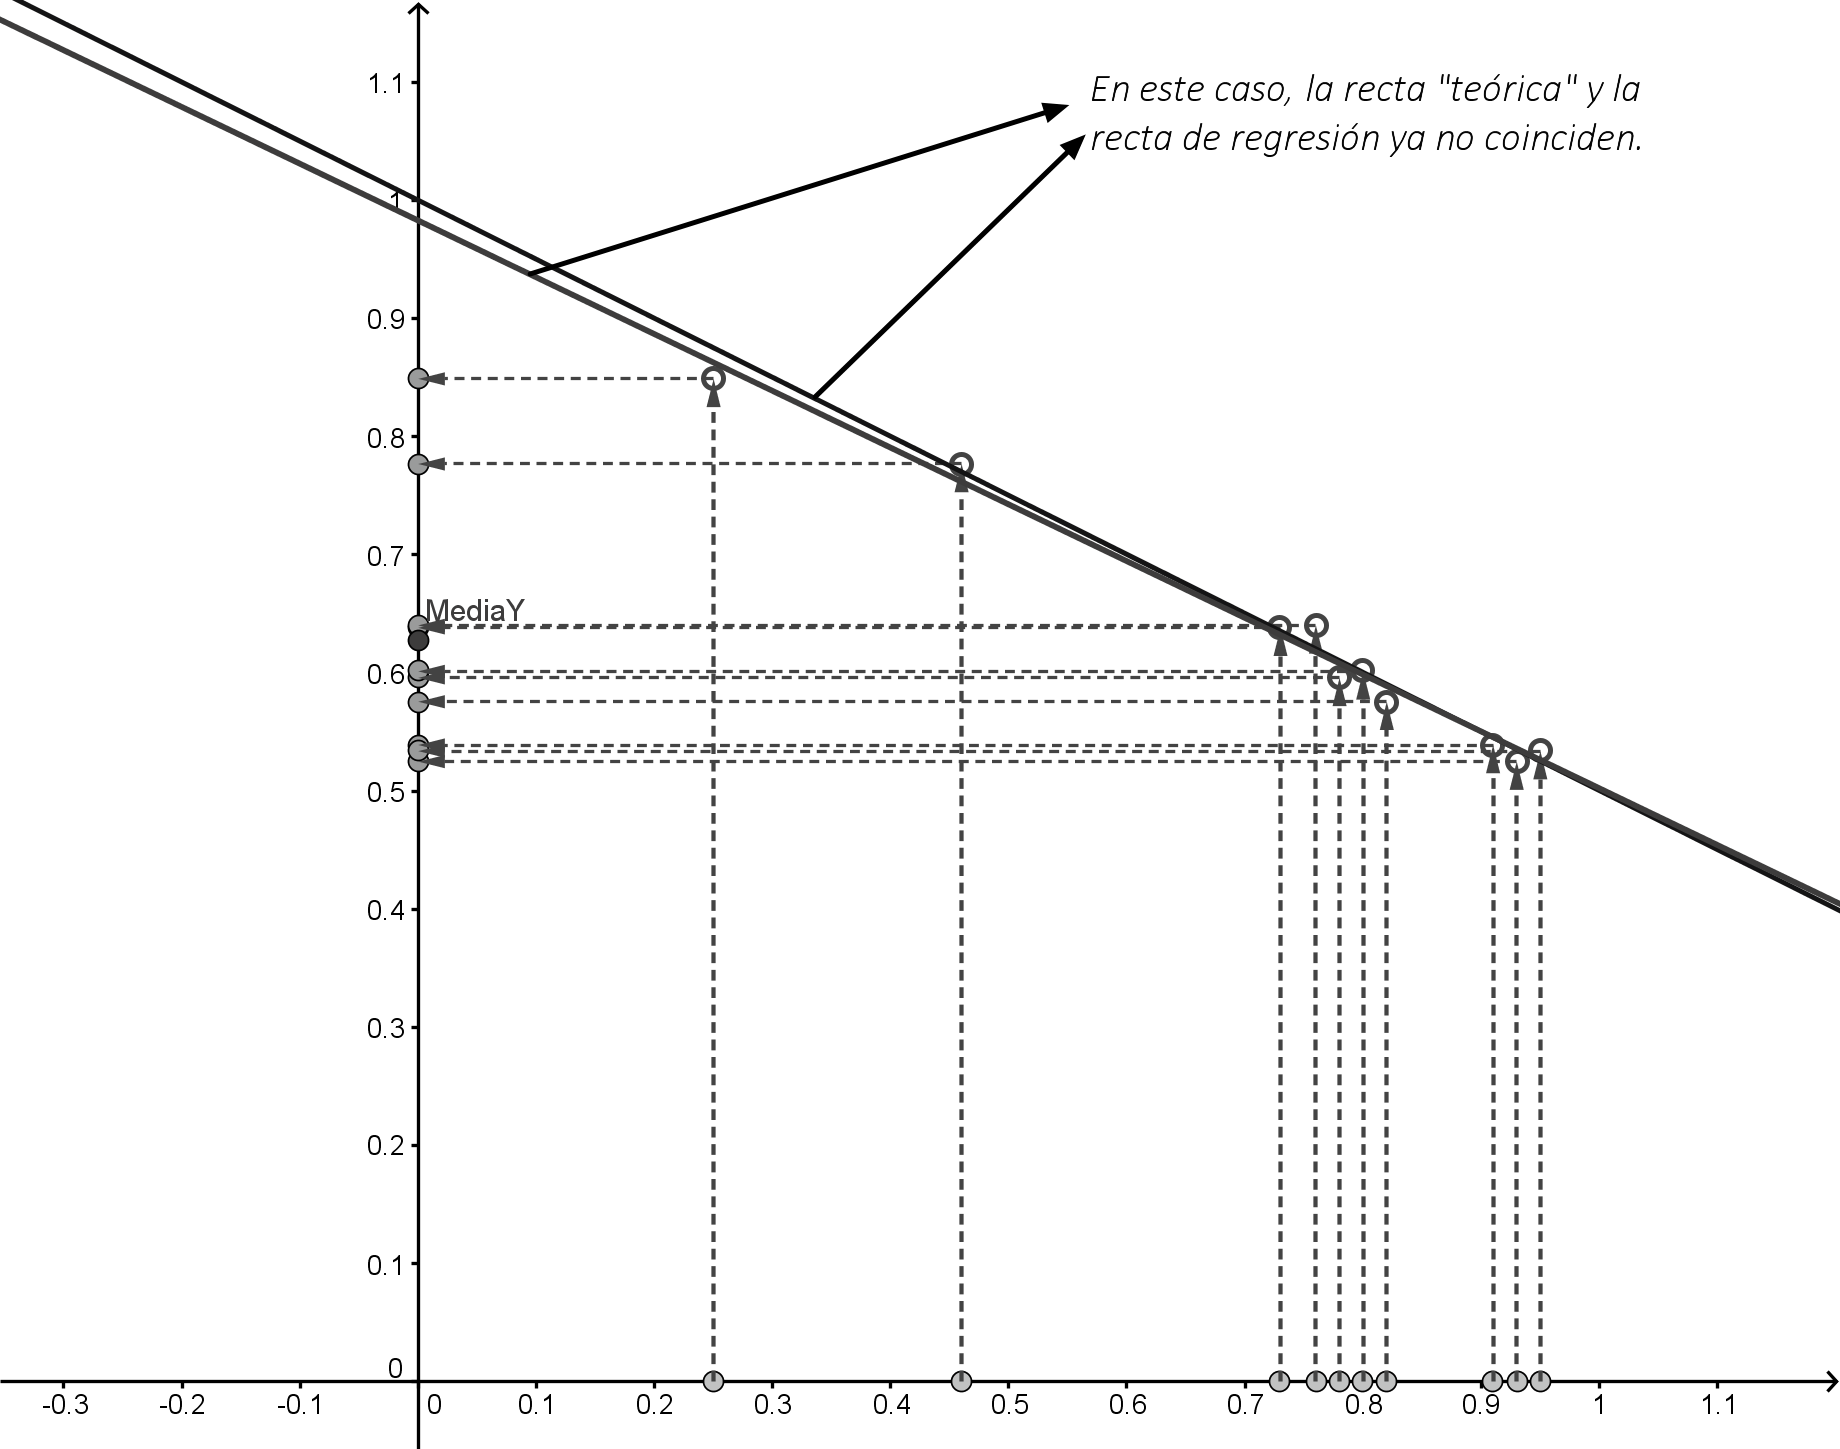
\includegraphics[height=10cm]{../fig/Cap10-Anova02-bn.png}
\end{bn}
\caption{Anova en la regresión. Caso ``ruidoso'': ahora la dispersión de $y$ {\bf no} se explica completamente por el efecto de la recta, y es necesario tener en cuenta el componente aleatorio que interviene en la generación de los valores $y_i$.}
\label{cap10:fig:Anova02}
\end{center}
\end{figure}

Supongamos ahora que tenemos otra lista de valores $y_1,\ldots, y_{10}$, que se han obtenido de los $x_i$ usando la misma recta $y=1-\dfrac{x}{2}$, pero introduciendo cierto nivel de ruido aleatorio en el proceso. En la próxima sección daremos más detalles, y en el Tutorial10 aprenderemos una forma de hacer esta simulación con el ordenador. Los puntos que hemos obtenido aparecen en la Tabla \ref{cap10:tabla:Anova01ruidosos}, y en la Figura \ref{cap10:fig:Anova02} (pág. \pageref{cap10:fig:Anova02}).

\begin{table}[ht]
\centering
\begin{tabular}{rrrrrrrrrrr}
  \hline
$i$ & 1 & 2 & 3 & 4 & 5 & 6 & 7 & 8 & 9 & 10 \\
  \hline
$x_i$ & 0.25 & 0.46 & 0.73 & 0.76 & 0.78 & 0.80 & 0.82 & 0.91 & 0.93 & 0.95 \\
$y_i$ & 0.85 & 0.78 & 0.64 & 0.64 & 0.60 & 0.60 & 0.58 & 0.54 & 0.52 & 0.53 \\
   \hline
\end{tabular}
\caption{Puntos ``ruidosos'' del Ejemplo \ref{cap10:ejem:Anova01}}
\label{cap10:tabla:Anova01ruidosos}
\end{table}

\noindent En este caso, la media y la dispersión total de los $y_i$ son
\[\bar y\approx 0.6274,\qquad \displaystyle\sum_{i=1}^{n}(y_i-\bar y)^2=(n-1)\cdot s^2(y)\approx 0.1031692,\]
pero ahora esa varianza ya no se puede explicar usando sólo la varianza de los $x_i$ y la recta. Si calculamos, para estos valores, el último término de la identidad \ref{cap10:ecu:AnovaparaRegresion}, se tiene:
\[\sum_{i=1}^n(\hat y_i-\bar y)^2=\sum_{i=1}^n\left((1-\dfrac{x_i}{2})-0.6274\right)^2,\]
y sustituyendo los valores de los $x_i$, obtenemos,
\[\sum_{i=1}^n(\hat y_i-\bar y)^2\approx 0.1016513\]
que no coincide con el cálculo de $(n-1)\cdot s^2(y)\approx 0.1031692$. De hecho, es menor. La razón es que, en este caso, falta la contribución del ruido aleatorio a la dispersión de los valores $y_i$. Para obtenerla, necesitamos calcular los puntos $\hat y_i$, y para eso es preciso calcular la recta de regresión. Que, a causa precisamente de ese componente ruidoso, no coincidirá exactamente con el modelo ``teórico'' $y=1-\dfrac{x}{2}$ que hemos usado). La recta de regresión que se obtiene es, aproximadamente:
\[y=0.98-0.48\cdot x.\]
Con esta recta, sustituyendo los $x_i$, obtenemos la Tabla \ref{cap10:tabla:Anova01predichos}.
\begin{table}[htb]
\centering
\begin{tabular}{rrrrrrrrrrr}
  \hline
$i$ & 1 & 2 & 3 & 4 & 5 & 6 & 7 & 8 & 9 & 10 \\
  \hline
$\hat y_i$ & 0.86 & 0.76 & 0.63 & 0.62 & 0.61 & 0.60 & 0.59 & 0.55 & 0.54 & 0.53 \\
   \hline
\end{tabular}
\label{cap10:tabla:Anova01predichos}
\caption{Los valores $\hat y_i$ que predice la recta de regresión, en la segunda parte del Ejemplo \ref{cap10:ejem:Anova01}. }
\end{table}
Y usando esos valores $\hat y_i$, podemos calcular el error cuadrático
\[EC=\sum_{i=1}^n(y_i-\hat y_i)^2\approx 0.001518\]
Puedes comprobar que el error cuadrático es justo la diferencia entre la dispersión total de $y$, y el último término de la identidad \ref{cap10:ecu:AnovaparaRegresion}. Es decir:
\[
\begin{array}{ccccc}
 \displaystyle\sum_{i=1}^{n}(y_i-\bar y)^2 &=&\mbox{EC} & + & \sum_{i=1}^n(\hat y_i-\bar y)^2\\
                  0.1031692                &=&0.001518  & + &          0.1016513
\end{array}
\]
confirmando en este caso la identidad \ref{cap10:ecu:AnovaparaRegresion}.
\qed
\end{ejemplo}

La conclusión, apoyada por este ejemplo, es que podemos interpretar los términos que aparecen en la identidad \ref{cap10:ecu:AnovaparaRegresion} así:
\[
        \underbrace{ \displaystyle\sum_{i=1}^{n}(y_i-\bar y)^2}_{\left(\mbox{\small dispersión total de }y\right)}=
        \underbrace{\displaystyle\sum_{i=1}^n(y_i-\hat y_i)^2}_{\left(\mbox{\small dispersión aleatoria }EC\right)}+
        \underbrace{\displaystyle\sum_{i=1}^n(\hat y_i-\bar y)^2}_{\left(\mbox{\small dispersión explicada por la regresión}\right)}
\]
Es frecuente encontrarse versiones de esta identidad como esta:
\begin{equation}\label{cap10:ecu:versionSSidentidadAnova}
SST = SS_{\mbox{\tiny residual}} + SS_{\mbox{\tiny modelo}}
\end{equation}
donde $SS$ es la abreviatura de la frase en inglés {\em sum of squares}, {\sf suma de cuadrados}\index{suma de cuadrados, $SS$}, y cada término de la identidad tiene este significado:
\begin{itemize}
  \item $SST$ (la $T$ es de {\em Total}) es la suma de cuadrados total\index{$SST$}, el término $\displaystyle\sum_{i=1}^{n}(y_i-\bar y)^2$ que representa la dispersión total de $y$.
  \item $SS_{\mbox{\tiny residual}}$ (recuerda que los residuos son las diferencias $(y_i-\hat
      y_i)$). Este es el término $EC=\displaystyle\sum_{i=1}^n(y_i-\hat y_i)^2$, el error que
      nosotros hemos identificado con la componente aleatoria o ruidosa de la dispersión de los
      valores $y_i$. También podemos decir que es la parte de la dispersión {\em no explicada}
      por el modelo de regresión lineal (es decir, por la recta).
  \item $SS_{\mbox{\tiny modelo}}$ es el término $\displaystyle\sum_{i=1}^n(\hat y_i-\bar y)^2$,
      que hemos identificado con la parte de la dispersión de $y$ que se explica simplemente por
      el hecho de que existe ese modelo teórico de regresión, basado en una recta.

\end{itemize}

\paragraph{Advertencia sobre la notación con SST, SSE, SSR, etc.}
\label{cap10:parag:AdvertenciaSSE} En la literatura en inglés  estos términos a menudo se
representan con los símbolos $SSE$ y$SSR$. Pero, en nuestra (minoritaria) opinión, esa notación
resulta ambigua. Para muchos autores, la $R$ en $SSR$ proviene del inglés {\em regression}, y
se refiere a lo que nosotros llamamos el modelo. Mientras que la $E$ de $SSE$ proviene de {\em
error}, y se refiere a lo que nosotros llamamos el residuo. Pero es fácil interpretar también la $R$
en $SSR$ como {\em residual} (y así se hace en algunos libros). Hemos encontrado muchas variantes
sobre esta notación, en el contexto de la regresión y en el del Anova que veremos en el próximo
capítulo,  con símbolos como $SSTO$ (de {\em total}), $SSM$ (de {\em model}), e incluso $SST$ con $T$ {!`}de {\em treatments}, tratamientos!. En una situación como esta, lo único sensato que podemos recomendar
es ejercer la prudencia, y al utilizar cualquier referencia o programa de ordenador, comprobar con
cuidado cuál es la terminología que se está usando (por ejemplo, se puede ejecutar un ejemplo con
resultados conocidos).

\subsubsection{Prueba de la identidad Anova \ref{cap10:ecu:AnovaparaRegresion}}
\noindent{\bf Opcional: esta sección puede omitirse en una primera lectura.}\\

Vamos a probar la identidad Anova (Ecuación \ref{cap10:ecu:AnovaparaRegresion}, pág. \pageref{cap10:ecu:AnovaparaRegresion}). Recuerda que esa identidad era:
\[
    \displaystyle\sum_{i=1}^{n}(y_i-\bar y)^2 =
    \sum_{i=1}^n(y_i-\hat y_i)^2 +\sum_{i=1}^n(\hat y_i-\bar y)^2
\]
Prácticamente nuestra única razón para incluir la demostración es que muchos textos de nivel introductorio la omiten. Así que, como referencia, hemos preferido mantenerla. Secundariamente, el análisis de la prueba ayuda a entender mejor que esa identidad va inseparablemente  unida al método de mínimos cuadrados. Naturalmente, teniendo esto en cuenta, este apartado tiene un interés particularmente técnico, y el lector no interesado puede omitirlo sin apenas ninguna consecuencia.

Empezamos con  el viejo truco de sumar y restar una misma cantidad, en este caso $\hat y_i$,  para acercarnos a nuestro objetivo:
\[
    \displaystyle\sum_{i=1}^{n}(y_i-\bar y)^2 =
    \displaystyle\sum_{i=1}^{n}\left[(y_i - \hat y_i) + (\hat y_i - \bar y)\right]^2.
\]
Desarrollando el cuadrado del miembro derecho tenemos:
\begin{eqnarray*}
    \displaystyle\sum_{i=1}^{n}(y_i-\bar y)^2  & = &
       \displaystyle\sum_{i=1}^{n}\left[(y_i - \hat y_i)^2  +
    (\hat y_i - \bar y)^2 +
    2(y_i - \hat y_i)\cdot (\hat y_i - \bar y)
       \right]
    \\
    & = &
    \displaystyle\sum_{i=1}^{n}(y_i - \hat y_i)^2  +
    \displaystyle\sum_{i=1}^{n}(\hat y_i - \bar y)^2 +
    2\cdot\displaystyle\sum_{i=1}^{n} (y_i - \hat y_i)\cdot (\hat y_i - \bar y).
\end{eqnarray*}
%\[
%    \displaystyle\sum_{i=1}^{n}(y_i-\bar y)^2 =
%    \displaystyle\sum_{i=1}^{n}(y_i - \hat y_i)^2  +
%    \displaystyle\sum_{i=1}^{n}(\hat y_i - \bar y)^2 +
%    2\cdot\displaystyle\sum_{i=1}^{n} (y_i - \hat y_i)\cdot (\hat y_i - \bar y)
%\]
y, para que la demostración esté completa, lo que tenemos que probar es que el último término es nulo:
\[
    \displaystyle\sum_{i=1}^{n} (y_i - \hat y_i)\cdot (\hat y_i - \bar y)=0.
\]
Para demostrar esto vamos a sustituir en el primer paréntesis $\hat y_i$ usando la Ecuación \ref{cap10:ecu:ValorPrediceRectaRegresion} (pág. \pageref{cap10:ecu:ValorPrediceRectaRegresion}). Es decir, haremos:
\[y_i-\hat y_i = (y_i - \bar y) - b_1\cdot (x_i-\bar x).\]
En el segundo paréntesis, en cambio, usaremos el hecho de que
\[
\begin{cases}
\hat y_i= b_0 + b_1\cdot \hat x_i\\
\bar y = b_0 + b_1\cdot \bar x,
\end{cases}
\]
de donde, si restamos miembro a miembro ambas expresiones, tenemos
\[\hat y_i - \bar y = b_1\cdot(\hat x_i - \bar x).\]
Con todo esto, tenemos:
\begin{eqnarray*}
    \displaystyle\sum_{i=1}^{n} (y_i - \hat y_i)\cdot (\hat y_i - \bar y)  & = &
     \displaystyle\sum_{i=1}^{n} \left[(y_i - \bar y) - b_1\cdot (x_i-\bar x)\right]\cdot b_1\cdot(\hat x_i - \bar x)
    \\
    & = &
    b_1\cdot \displaystyle\sum_{i=1}^{n} (y_i - \bar y)\cdot (x_i-\bar x)-
b_1^2\cdot \displaystyle\sum_{i=1}^{n} (x_i-\bar x)^2\\
    & = &
    b_1\cdot(n-1)\cdot \Cov(x,y) - b_1^2\cdot(n-1)\cdot s^2(x)
\end{eqnarray*}
%\[
%    \displaystyle\sum_{i=1}^{n} (y_i - \hat y_i)\cdot (\hat y_i - \bar y)=
%    \displaystyle\sum_{i=1}^{n} \left((y_i - \bar y) - b_1\cdot (x_i-\bar x)\right)\cdot b_1\cdot(\hat x_i - \bar x)=
%\]
%\[
%=
%b_1\cdot \displaystyle\sum_{i=1}^{n} (y_i - \bar y)\cdot (x_i-\bar x)-
%b_1^2\cdot \displaystyle\sum_{i=1}^{n} (x_i-\bar x)^2=
%\]
%\[
%b_1\cdot(n-1)\cdot \Cov(x,y) - b_1^2\cdot(n-1)\cdot s^2(x).
%\]
Y ahora basta sustituir $b_1$ por su valor según la Ecuación \ref{cap10:ecu:RectaRegresionPendienteOrdenadaOrigen} (pág. \pageref{cap10:ecu:RectaRegresionPendienteOrdenadaOrigen}) para comprobar que el resultado es, como queríamos, igual a $0$.

Si has leído la Sección \ref{cap10:subsec:RegresionOrtogonal} (pág. \pageref{cap10:subsec:RegresionOrtogonal}) sobre regresión ortogonal, queremos aprovechar para señalar que esta demostración de la identidad Anova \ref{cap10:ecu:AnovaparaRegresion} que hemos visto se basa en el error cuadrático, y en el cálculo de $b_1$ para la recta del modelo de mínimos cuadrados. Por lo tanto, esa identidad Anova sólo tiene sentido cuando se aplica ese modelo de regresión. Si se aplica el modelo de regresión ortogonal, los puntos predichos del sistema cambian, y esta identidad ANOVA ya no se aplica. Volveremos sobre este asunto en el Capítulo \ref{cap:RegresionLogistica}, al analizar la estructura del error en la Regresión Logística.

\subsection{Coeficiente $r$ de correlación lineal de Pearson.}
\label{cap10:subsec:CoeficienteRPearson}

Con la descomposición de la dispersión de $y$ que hemos obtenido, estamos por fin en condiciones de obtener una estimación de la calidad de la recta de regresión, que sea independiente de la escala del problema (como hemos discutido al comienzo de esta Sección \ref{cap10:sec:AnovaCoeficienteCorrelacion}).

Para hacerlo, partimos otra vez de la identidad \ref{cap10:ecu:AnovaparaRegresion}
\[
\displaystyle\sum_{i=1}^{n}(y_i-\bar y)^2 = \mbox{EC}+\sum_{i=1}^n(\hat y_i-\bar y)^2
\]
y dividimos todos sus términos por el de la izquierda, el que representa la dispersión total de $y$. Se obtiene:
\begin{equation}\label{cap10:ecu:ecuacionAnovaAdimensional}
1 =
\dfrac{\mbox{EC}}{\displaystyle\sum_{i=1}^{n}(y_i-\bar y)^2}
+
\dfrac{\displaystyle\sum_{i=1}^n(\hat y_i-\bar y)^2}{\displaystyle\sum_{i=1}^{n}(y_i-\bar y)^2}
\end{equation}
Esta división nos garantiza que los dos sumandos de la derecha son {\em adimensionales}. En particular, son números que no dependen de la escala del problema, como queríamos. Ambos son, además, cantidades positivas. Así que estamos repartiendo la unidad, el $1$ de la izquierda de la igualdad, en dos sumandos positivos. De los cuales, el primero (residual) está relacionado con la parte aleatoria o ruidosa de los datos, mientras que el segundo corresponde a la parte que queda explicada por el modelo de regresión (la recta). En particular, parece ser que la recta será tanto mejor, cuanto más grande sea este segundo sumando y, por tanto, más pequeño sea el primero.

Para expresar esto de otra manera, vamos a recordar aquí la Ecuación \ref{cap10:ecu:ValorPrediceRectaRegresion} (pág. \pageref{cap10:ecu:ValorPrediceRectaRegresion}) de la recta de regresión:
\[\hat y_i-\bar y = \dfrac{\Cov(x,y)}{s^2(x)}\cdot (x_i-\bar x)\]
Si sustituimos esto en el numerador del último sumando de la Ecuación \ref{cap10:ecu:ecuacionAnovaAdimensional} obtenemos:
\[1 =
\dfrac{\mbox{EC}}{\displaystyle\sum_{i=1}^{n}(y_i-\bar y)^2}
+
\dfrac{\displaystyle\sum_{i=1}^n\left(\dfrac{\Cov(x,y)}{s^2(x)}\cdot (x_i-\bar x) \right)^2}{\displaystyle\sum_{i=1}^{n}(y_i-\bar y)^2}
\]
Reorganizando esto un poco (es necesario dividir el numerador y denominador de esa fracción por
$n-1$) llegamos a:
\begin{equation}%\label{cap10:ecu:ParaDefinirCoeficientePearson}
1 = \dfrac{\mbox{EC}}{\displaystyle\sum_{i=1}^{n}(y_i-\bar y)^2} + \left(
\dfrac{\Cov(x,y)}{s(x)\cdot s(y)} \right)^2
\end{equation}
El término que aparece entre paréntesis, nos va permitir relacionar la calidad de la recta con la covarianza de $x$ e $y$. Por eso es especialmente importante.
    \begin{center}
    \fcolorbox{black}{Gris025}{
    \begin{minipage}{12.5cm}
        \begin{center}
        %%%%%%%%%%%%%%%%%%%%%%%%%%%%%%%%%%%%%%%
        {\bf Coeficiente de correlación lineal de Pearson.}\index{coeficiente de correlación lineal de Pearson}
        \index{coeficiente de correlación de Pearson}
        \end{center}
       %%%%%%%%%%%%%%%%%%%%%%%%%%%%%%%%%%%%%%%
         Es el valor $r$ definido mediante:
         \begin{equation}\label{cap10:ecu:CoeficienteRegresionPearson}
         r=\dfrac{\Cov(x,y)}{{s(x)\cdot s(y)}}
         \end{equation}
         Recuerda que $\Cov(x,y)$ es la covarianza (muestral) de $x$ e $y$, definida en la Ecuación \ref{cap10:ecu:Covarianza} (pág. \pageref{cap10:ecu:Covarianza}). También lo denotaremos por $\operatorname{Cor}(x,y)$, y diremos que $r$ es la {\sf correlación}\index{correlación} de $x$ e $y$.
       %%%%%%%%%%%%%%%%%%%%%%%%%%%%%%%%%%%%%%%
    \end{minipage}
    }
    \end{center}
Este coeficiente debe su nombre a Karl Pearson, uno de los estadísticos más influyentes de
comienzos del siglo XX (más información en el enlace [\,\ref{enlace0021}\,]\label{enlace0021a} de la Wikipedia, en inglés), a quien ya hemos nombrado antes, en relación con los intervalos de confianza de la Sección \ref{cap08:subsec:MetodoExactoBinomial} (pág. \pageref{cap08:subsec:MetodoExactoBinomial}).

Usando la definición de $r$ podemos escribir:
\[1 =\dfrac{\mbox{EC}}{\displaystyle\sum_{i=1}^{n}(y_i-\bar y)^2}+r^2\]
o también, dividiendo numerador y denominador de la primera fracción por $n-1$,
\begin{equation}\label{cap10:ecu:interpretacionCoeficienteCorrelacion}
1 =\dfrac{\mbox{ECM}}{s^2(y)}+r^2,
\end{equation}
donde $ECM$ es el error cuadrático medio, que definimos en la Ecuación \ref{cap10:ecu:ECM} (pág.
\pageref{cap10:ecu:ECM}). Ahora queda claro por que, entonces, usamos $n-1$ para definir $ECM$.

\subsubsection{Interpretación de $r$. Correlación e independencia.}

La Ecuación \ref{cap10:ecu:interpretacionCoeficienteCorrelacion} nos permite interpretar $r$. Es un número, relacionado con la covarianza, que tomará valores entre $-1$ y $1$. Y tiene la propiedad de que {\em cuanto más cerca de 0 está $r^2$, peor es el ajuste de la recta de regresión a los
datos}.  A veces se presentan reglas como ``el ajuste es bueno si $r^2$ es mayor que...'', y la cantidad que sea. Desaconsejamos el uso de ese tipo de recetas: es mucho mejor utilizar otro tipo de herramientas, que exploraremos en el Tutorial10, para comprobar la calidad del ajuste que ofrece la recta en cada caso. Las dos ideas generales que ofrecemos al lector son estas:
\begin{itemize}
  \item Si el ajuste es bueno, el valor de $r$ (y de $r^2$) debe estar cerca de $1$. Ten en cuenta siempre que $r^2$ es más pequeño que $r$, porque $0<r<1$. Pero la interpretación contraria puede ser engañosa: hay ejemplos en los que un valor de $r$ relativamente alto se corresponde con un ajuste poco satisfactorio.
  \item Un valor de $r$ pequeño nos dice siempre que el ajuste de la recta a los datos es malo. Pero eso no significa gran cosa si no hacemos un buen análisis exploratorio de los datos. Veremos, en el Tutorial10, ejemplos en los que un único valor, que puede ser un {\em valor atípico} en el sentido del Capítulo \ref{cap:ValoresCentralesDispersion} (ver pág. \pageref{cap02:subsubsec:RangoIntercuartilico}), puede tener una gran influencia en la calidad del ajuste. En esos casos, el análisis exploratorio de los datos nos permite a veces detectar esos valores, y decidir si queremos hacer un ajuste alternativo, sin tenerlos en cuenta.
\end{itemize}

Comenzamos este capítulo hablando de la noción de correlación entre dos variables (recuerda la Figura \ref{cap10:fig:Herrerillo02}, pág. \pageref{cap10:fig:Herrerillo02}, y la discusión que la acompañaba). Y dijimos que era necesario dar una idea más precisa de la correlación. El coeficiente de correlación $r$ nos permite mejorar esa precisión. Los valores de dos variables están {\sf fuertemente correlacionados}\index{correlación fuerte} si el valor de $r$ es cercano a $1$.

El signo de $r$ se corresponde con el de la pendiente $b_1$ de la recta de regresión, y tiene la misma interpretación que esa pendiente. También coincide, por lo tanto, el signo de la covarianza. En particular, si $r$ es $0$ (lo que apunta a que el ajuste es muy malo), entonces la covarianza es $0$. Esto nos permite interpretar la covarianza como una cierta medida de la relación, o dependencia, que existe entre los valores de las dos variables. Es un buen momento para que revises los valores de la covarianza que incluimos la final de los Ejemplos \ref{cap10:ejem:RectaMalaAproximacion01} (pág. \pageref{cap10:ejem:RectaMalaAproximacion01})y \ref{cap10:ejem:RectaMalaAproximacion02} (pág. \pageref{cap10:ejem:RectaMalaAproximacion02}), porque ahora entendemos lo que nos estaban diciendo esas covarianzas tan bajas.


Y, ya que hablamos de dependencia, es posible que el lector haya recordado, en algún momento de este capítulo, la discusión sobre independencia de variables aleatorias que tuvimos en la Sección \ref{cap04:sec:IndependenciaVariablesAleatoriasDiscretas} del Capítulo \ref{cap:TeoremaCentralLimite}. En efecto, existe una relación entre ambas nociones. Pero hay que tener presente que en aquel capítulo hablábamos de {\em variables aleatorias}, que son conceptos teóricos, mientras que en este estamos hablando, desde el principio, de {\em muestras} de esas variables. Para establecer la conexión con precisión tendríamos que dar la versión teórica de algunas de las nociones que hemos visto en este capítulo. En particular, tendríamos que definir la covarianza de dos variables aleatorias, $\Cov(X,Y)$. En este capítulo hemos usado la covarianza de dos vectores (muestras) $x$ e $y$, con valores concretos. Es una diferencia similar a la que hay entre $\mu$ y el valor de $\bar x$ en una muestra concreta. Pero cuando las cosas se hacen con cuidado, y se usa la definición teórica de $\Cov(X,Y)$, se obtiene un resultado que cabría esperar:

\begin{itemize}
 \item Si dos variables $X$ e $Y$ son independientes, entonces $\Cov(X,Y)=0$.
\end{itemize}

Cuando dos variables cumplen $\Cov(X,Y)=0$, decimos que son {\sf variables incorreladas}\index{incorreladas, variables aleatorias} (en inglés, {\em uncorrelated}\index{uncorrelated}).  Lo que, sin duda, resulta un poco más inesperado es este resultado negativo:

\begin{itemize}
 \item El hecho de que dos variables $X$ e $Y$ sean incorreladas, no implica necesariamente que sean independientes. Es decir, hay variables que son a la vez dependientes e incorreladas.
\end{itemize}

\subsubsection*{Correlación y causalidad.}
\label{cap10:subsubsec:CorrelacionVsCausalidad}

Así pues, dependencia y correlación son conceptos emparentados, pero distintos. Hay todavía un tercer concepto, el de {\sf causalidad}\index{causalidad vs correlación}, que a menudo se mezcla con el concepto de correlación. No queremos cerrar este capítulo sin repetir uno de los {\em mantras} que cualquier estudiante de Estadística debe grabar en su memoria:

    \begin{center}
        \fcolorbox{black}{Gris025}{\begin{minipage}{6cm}
        \begin{center}
            {\sf La correlación no implica la causalidad.}
        \end{center}
        \end{minipage}}
    \end{center}

Son frecuentes los ejemplos de mal uso de la Estadística, en los que alguien, después de observar que los valores de dos variables $X$ e $Y$ están fuertemente correlacionados, argumenta que $X$ causa $Y$ o viceversa. Hay numerosos ejemplos que prueban que este tipo de argumentación, si no viene respaldada por algún {\em mecanismo} que vincule a $X$ (por ejemplo) como causa de $Y$, carece por completo de sentido. Uno de los más clásicos es la fuerte correlación que hay entre las variables $X=$``peso''  $Y=$``altura'' en las personas. Los valores de las dos variables están ligados de tal manera, en la población, que estadísticamente esperamos que una persona alta pese más que una baja. Pero la relación no es desde luego causal: el peso no {\em causa} la altura. Decir eso sería tanto como decir que si ganamos peso, ganamos en altura.

A menudo, este tipo de confusiones se deben a que se ha interpretado mal el sentido del vínculo entre dos variables, o a que no se ha tenido en cuenta la presencia de una tercera variable, con la que se relacionan ambas $X$ e $Y$, y que si tienen un efecto causal sobre ambas. En otro ejemplo clásico, existe una fuerte correlación entre el recuento diario de personas que sufren crisis alérgicas, y las ventas de cremas de protección solar. Pero no tiene sentido deducir que ``las cremas solares causan las crisis alérgicas ({!`}{!`}en personas que ni siquiera las usan, ni se exponen a ellas!!)''. El {\em mecanismo} que vincula estas dos variables es que tanto las crisis alérgicas como el uso de cremas solares están ligados al tiempo más soleado, propio de la primavera o verano, de manera que cuando luce el sol, hay más alergias y se usa más crema solar. Es el sol el que {\em causa} ambos procesos.

En cualquier caso, y como despedida de este capítulo, no creemos que nadie haya encontrado una
mejor explicación de la relación entre correlación y causalidad que Randall Munroe, el siempre
ocurrente autor de la tira cómica {\tt xkcd}, que hizo su particular interpretación en la viñeta
que encontrarás en el enlace [\,\ref{enlace0022}\,]\label{enlace0022a}.


\section{Inferencia en la regresión lineal.}
\label{cap10:sec:InferenciaRegresionLineal}
\noindent{\bf Opcional: esta sección puede omitirse en una primera lectura.}\\


Empecemos recordando que la recta de regresión $y=b_0+b_1\cdot x$ que hemos localizado en
la anterior sección es,
%    \[(y-\bar y)=\dfrac{{\Cov(x,y)}}{V_x}(x-\bar x),\]
 \[ (y-\bar y)= \dfrac{\Cov(x,y)} {s^2(x)}\cdot (x-\bar x),\]
siendo
%\[\Cov(x,y)=\dfrac{\displaystyle\sum_{i=1}^{n}(x_i-\bar x)(y_i-\bar y)}{n}.\]
\[\Cov(x,y)=\dfrac{\displaystyle\sum_{i=1}^{n}(x_i-\bar x)(y_i-\bar y)}{n-1}\]
Como hemos visto, esta recta es, de entre todas las rectas posibles, la que mejor representa, desde el punto de vista estadístico, a la {\sf muestra} de $n$ puntos del plano:
    \[(x_1,y_1),(x_2,y_2),(x_3,y_3),\ldots,(x_n,y_n),\]
Y hemos aprendido que podemos usar $r$, el coeficiente de correlación de Pearson, para medir la
calidad de esa recta, {\em para describir esos $n$ puntos}. Pero, naturalmente, eso es sólo el
primer paso. Hemos destacado antes la palabra muestra, porque, en un problema típico, esos $n$
puntos serán sólo una muestra, tomada de una población, en la que que nos interesa estudiar el
modelo $Y \sim X$. Y, como  cabe suponer, cada muestra diferente que tomemos producirá una recta
distinta.

En la Figura \ref{cap10:fig:RectasRegresionDosMuestras} pueden verse dos muestras de una misma
población, una representada por los puntos redondos, y otra por las cruces rojas y las
correspondientes rectas de regresión: en azul con trazo continuo la de la primera población, y en
rojo con trazo discontinuo la de la segunda. Esa figura confirma lo que decíamos: cada muestra
puede producir una recta distinta, con valores distintos de $b_0$ y $b_1$.

\begin{figure}[htbp]
\begin{center}
\begin{enColor}
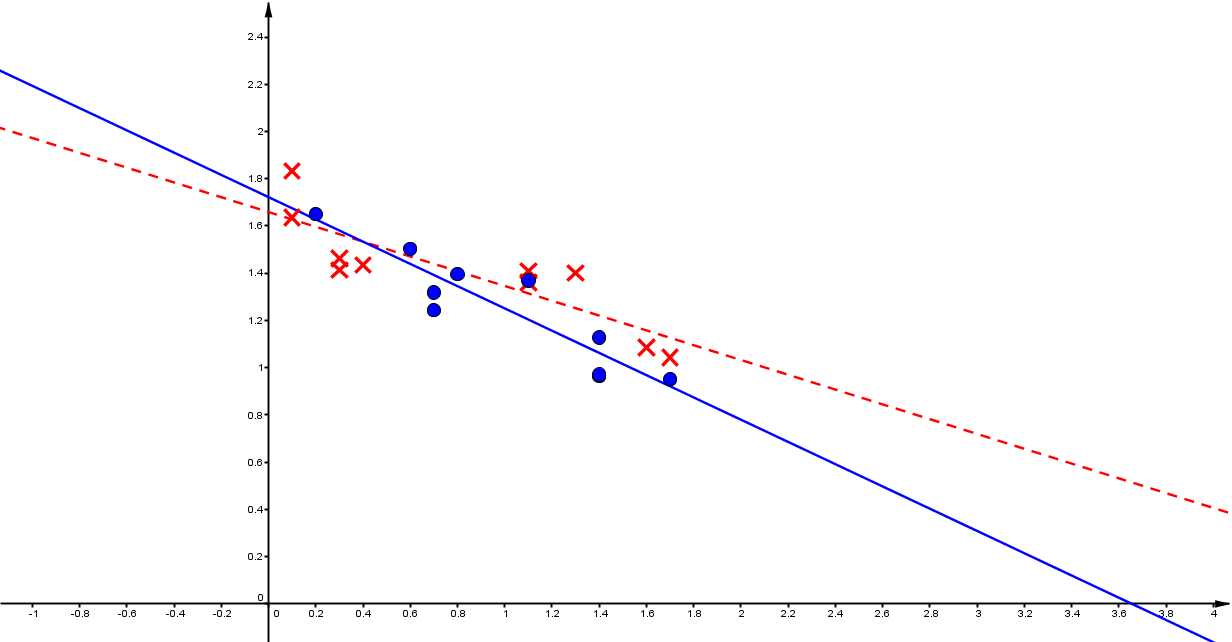
\includegraphics[width=12.5cm]{../fig/Cap10-RegresionMuestrasDistintas.png}
\end{enColor}
\begin{bn}
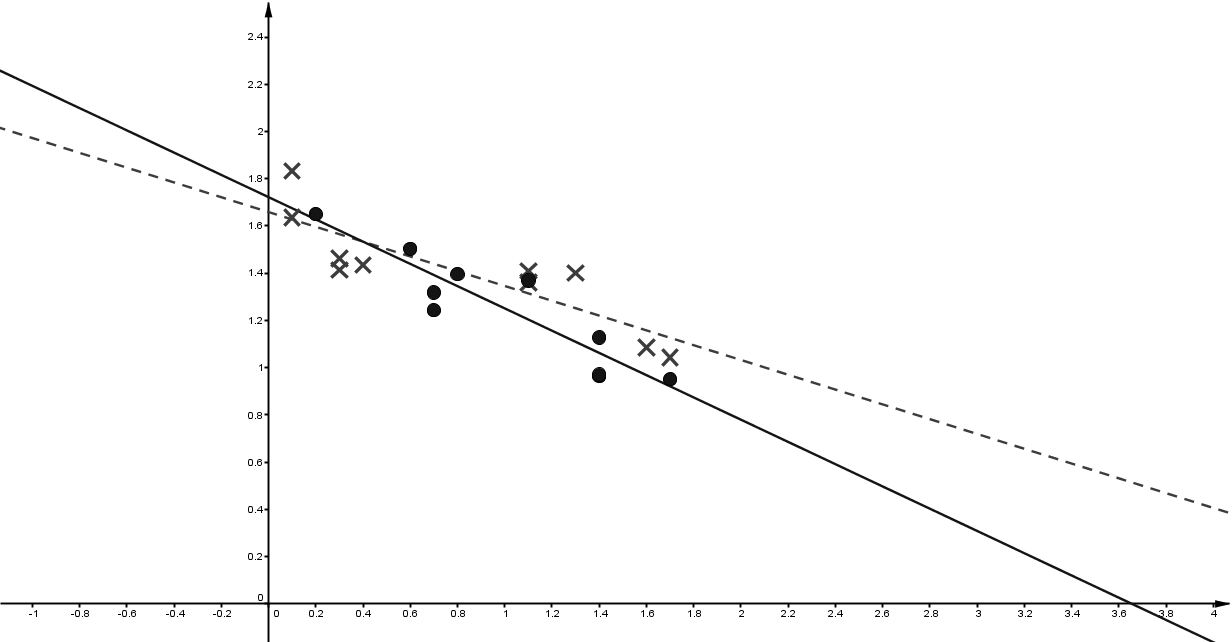
\includegraphics[width=12.5cm]{../fig/Cap10-RegresionMuestrasDistintas-bn.png}
\end{bn}
\caption{Rectas de regresión para dos muestras de una misma población.}
\label{cap10:fig:RectasRegresionDosMuestras}
\end{center}
\end{figure}


¿Y entonces? ¿Cuál es la recta ``buena'', la que debemos usar para representar el modelo $Y \sim
X$? Incluso antes de tener muy claro de qué estamos hablando, vamos a llamar
    \begin{equation}\label{cap10:ecu:rectaRegresionPoblacional}
        y=\beta_0 +\beta_1\cdot x
    \end{equation}
a esa {\sf recta de regresión teórica}\index{recta de regresión teórica}.  Como es habitual, usamos
letras griegas para referirnos a los parámetros poblacionales, $\beta_0$, $\beta_1$ para
distinguirlos de los parámetros $b_0$ y $b_1$ que corresponden a la muestra.

Antes de avanzar, queremos detenernos un momento, para ocuparnos de una posible duda que puede
estar surgiendo en el lector. ¿No habíamos construido ya el coeficiente $r$ para medir si el ajuste
de la recta era bueno? ¿Qué significa ahora esta discusión sobre la recta ``buena''? Es importante
entender que las rectas de las que hemos hablado hasta ahora en este capítulo tenían que ser las
mejores rectas posibles {\em para una muestra dada}. Ahora  estamos pensando en tomar distintas
muestras, y para cada una de ellas obtendremos la mejor recta posible. Pero puede ocurrir que la muestra sea ``mala'', en el sentido de poco representativa de la población. Y en ese caso, incluso la mejor
recta de una muestra mala seguirá siendo una recta mala, {\em cuando tratemos de usarla para
estudiar toda la población}.

¿Cómo se define esa recta teórica? A poco que se piense, la primera idea ingenua, que podría ser la
de usar {\em todos los puntos de la población}, no se puede aplicar directamente. Esto está claro, por ejemplo en el caso de poblaciones infinitas. Mirando la  Figura \ref{cap10:fig:InterpretacionErrorCuadratico}
(pág. \pageref{cap10:fig:InterpretacionErrorCuadratico}) trata de imaginarte cómo definiríamos el
error cuadrático con {\em infinitos puntos}. Esa idea ingenua contiene algo de verdad, pero
necesita bastante elaboración teórica. Lo que, sin duda, es cierto, es que para obtener un
resultado poblacional, tenemos que hacernos preguntas sobre la relación entre $X$ e $Y$ {\em en la
población}.

Hay varias formas de abordar ese tema, que corresponden a distintas formulaciones matemáticas. Para
entrar en algunas de esas formulaciones,
%y en especial, cuando se considera el Modelo II de regresión (ver la página \pageref{cap10:subsubsec:ModelosIyIIdeRegresion}),
sería necesario una discusión más profunda de las distribuciones conjuntas de dos variables, de las que nosotros sólo hemos hablado muy brevemente (y limitándonos al caso discreto) en la Sección \ref{cap04:sec:IndependenciaVariablesAleatoriasDiscretas} (pág. \pageref{cap04:sec:IndependenciaVariablesAleatoriasDiscretas}) del Capítulo \ref{cap:VariablesAleatorias}. Así que vamos a quedarnos, por tanto, con un modelo muy básico, pero aún así muy útil.

\subsection{Modelo de regresión lineal simple.}
\label{cap10:subsec:modeloRegresionLinealSimple}

Tenemos que dar una descripción de la relación entre $X$ e $Y$ que nos permita interpretar los
parámetros $\beta_0$ y $\beta_1$. El modelo que vamos a utilizar para describir esa relación es
este.  Supondremos que para cada valor fijo $x_0$ de la variable $x$ tenemos una variable aleatoria
normal $Y_{x_0}$ de tipo
\begin{equation}\label{cap10:ecu:modeloRegresionLinealSimple}
Y_{x_0}\sim N(\beta_0+\beta_1\cdot x_0,\sigma),
\end{equation}
donde $\sigma$ es la misma, independientemente de $x_0$. Esta suposición se denomina {\sf
homogeneidad de las varianzas}\index{homogeneidad de las varianzas} (o también con la palabreja
{\sf homocedasticidad}\index{homocedasticidad en la regresión}). Tanto la suposición de una
distribución normal, como la suposición de homogeneidad de las varianzas son, desde luego,
simplificaciones. Y en el apartado \ref{cap10:subsec:VerificandoCondicionesModeloRegresionLinealSimple} (pág. \pageref{cap10:subsec:VerificandoCondicionesModeloRegresionLinealSimple}) tendremos que preguntarnos cómo podremos comprobar que esas suposiciones se cumplen en un caso concreto.

Usando este modelo, interpretamos el punto $(x_1,y_1)$ suponiendo que $y_1$ es una observación de
$Y_{x_1}$, el punto $(x_2,y_2)$ suponiendo que $y_2$ es una observación de $Y_{x_2}$,etcétera,
hasta el punto $(x_n,y_n)$, para el que suponemos igualmente que $y_n$ es una observación de
$Y_{x_n}$. Esto es equivalente a suponer que nuestras observaciones se explican mediante este
modelo:
    \begin{equation}\label{cap10:ecu:InterpretacionModeloRegresionLinealSimple}
        y=
        \underbrace{\beta_0 +\beta_1\cdot x}_{\mbox{modelo}}
        +
        \underbrace{\phantom{\beta}\epsilon\phantom{\beta}}_{\mbox{ruido}},
        \quad\mbox{ siendo }\epsilon\sim N(0,\sigma).
    \end{equation}
Hemos llamado {\em modelo} a los términos que corresponden a la recta teórica, y {\em ruido} a un
término adicional $\epsilon$, que sigue una distribución normal centrada en $0$ y cuya varianza es
la varianza que hemos supuesto común a todas las $Y_{x_i}$. La terminología {\em modelo/ruido}
trata, obviamente, de recordar a la que hemos utilizado en la Ecuación
\ref{cap10:ecu:AnovaparaRegresion} de análisis de la varianza (pág.
\pageref{cap10:ecu:AnovaparaRegresion}).

En el Tutorial10 construiremos explícitamente modelos como este para poder experimentar con ellos,
y ver cómo se comportan.


La Figura \ref{cap04:fig:ModeloRegresionLinealSimple} ilustra la forma en la que se suele entender
esto. Como se ve en ella, para cada valor fijo $x_0$ hay asociada una copia local de la normal
$N(0,\sigma)$, centrada en el punto  $\hat y_0=\beta_0+\beta_1\cdot x_0$ (hemos llamado así al
valor $\hat y_0$ porque es el valor que la recta teórica predice para el valor $x_0$). Este modelo
encaja bien con situaciones como las del Ejemplo \ref{cap10:ejem:Anova01}, en las que descomponemos
en dos pasos el proceso que conduce del valor de $x$ al valor de $y$. Los dos pasos son:
\begin{itemize}
  \item Un paso en el que interviene la recta teórica del modelo, y obtenemos
    \[\hat y_0=\beta_0+\beta_1\cdot x_0.\]
    En este paso no hay componente aleatoria.
  \item Un segundo paso, en el que al valor $\hat y_0$ le sumamos una {\em componente ruidosa}
      calculada con la normal $N(0,\sigma)$, y que es el valor que hemos llamado $\epsilon$. Este
      término, desde luego, es el que contiene la parte aleatoria o ruidosa del modelo.
\end{itemize}

    \begin{figure}[htb]
	\centering
	\begin{enColor}
    \includegraphics[width=12cm]{../fig/Cap10-ModeloRegresionLinealSimple.png}
	\end{enColor}
	\begin{bn}
    \includegraphics[width=12cm]{../fig/Cap10-ModeloRegresionLinealSimple-bn.png}
	\end{bn}
	\caption{Ilustración del modelo de regresión lineal simple.}
	\label{cap04:fig:ModeloRegresionLinealSimple}
    \end{figure}


% que permite calcular las probabilidades condicionadas del tipo \[P(Y\leq y|x=x_0)\]

En este modelo $b_0$ y $b_1$ son, evidentemente, estimadores de los parámetros $\beta_0$ y
$\beta_1$ de la recta teórica. Pero ahora, al tener una descripción mediante la distribución
normal, podemos usarla para hacer inferencia (intervalos de confianza y contrastes de hipótesis)
sobre los valores de $\beta_0$ y $\beta_1$. Ya sabemos que el primer paso de la inferencia es
siempre buscar el estadístico adecuado. No nos vamos a entretener en los detalles técnicos (que, una vez más,
recurren a una especie de tipificación; el lector interesado puede ver los detalles en las
referencias \cite{inferenciaIpinnaDurand} y \cite{garcia2009estadistica} de la Bibliografía), y nos
limitaremos a decir que el estadístico que se obtiene es:
    \begin{center}
    \fcolorbox{black}{Gris025}{
    \begin{minipage}{12.5cm}
        \begin{center}
        %%%%%%%%%%%%%%%%%%%%%%%%%%%%%%%%%%%%%%%
        {\bf Estadístico para $\beta_1$, la pendiente de la recta teórica de regresión.}
        \index{estadístico para $\beta_1$, pendiente en la regresión}
        \end{center}
       %%%%%%%%%%%%%%%%%%%%%%%%%%%%%%%%%%%%%%%
         El estadístico
         \begin{equation}\label{cap10:ecu:EstadisticoPendienteRectaRegresion}
         \Xi=\dfrac{b_1-\beta_1}{\sqrt{\dfrac{ECM}{(n-2)s^2(x)}}}
         \end{equation}
         sigue una distribución $t$ de Student con $n-2$ grados de libertad.
       %%%%%%%%%%%%%%%%%%%%%%%%%%%%%%%%%%%%%%%
    \end{minipage}
    }
    \end{center}

\subsubsection{El número de grados de libertad del modelo}
\label{cap10:subsubsec:NumeroGradosLibertadModelo}

Vamos a discutir, siquiera sea brevemente, por qué aparecen $n-2$ grados de libertad en este estadístico.  No te preocupes si la discusión no te queda clara en una primera lectura. Este es uno de esos temas en los que la comprensión se consigue con la práctica y con la acumulación de ejemplos donde se repiten las mismas ideas.

En general, en Estadística, el número de grados de libertad tiene que ver con el número de parámetros que se estiman en un modelo. Todavía no hemos visto suficientes ejemplos de modelos estadísticos como para entender con detalle lo que queremos decir con esto, pero podemos hacernos una idea inicial. En el modelo de regresión lineal simple que estamos estudiando, el de la Ecuación \ref{cap10:ecu:modeloRegresionLinealSimple}, aparecen dos parámetros, $\beta_0$ y $\beta_1$. Por eso, al trabajar con muestras de tamaño $n$, el número de grados de libertad es
\begin{equation}\label{cap10:ec:numerogradoslibertad}
(\mbox{tamaño muestral})-(\mbox{parámetros estimados del modelo})= n - 2.
\end{equation}
Veremos más ejemplos de este tipo de relaciones en el resto de capítulos de esta parte del curso. Pero, para tener una referencia más, mirando hacia atrás, la primera vez que hablamos de grados de libertad, en relación con la $t$ de Student, estábamos usando muestras de tamaño $n$ para estimar {\em la media} (y sólo la media) de una población normal. Y en ese caso teníamos:
\begin{equation*}
(\mbox{tamaño muestral})-(\mbox{parámetros estimados del modelo})= n - 1,
\end{equation*}
como recordarás. El {\em modelo}, en ese caso, se puede ver de esta manera:
\[X=\mu+\epsilon,\]
siendo $\epsilon$ un término de error, con distribución $N(0,\sigma)$. De esa forma, con el lenguaje que cada observación de $X$ se puede descomponer en la parte que explica el modelo (el valor $\mu$), más el {\em ruido} que representa $\sigma$.

\subsubsection{Intervalo de confianza para la pendiente}
\label{cap10:subsubsec:IntervaloConfianzaPendiente}

Volvamos a la inferencia sobre el modelo de regresión lineal simple. A partir del estadístico, y de la información sobre su distribución muestral, como en otras ocasiones, es fácil construir los intervalos de confianza y contrastes de hipótesis.

    \begin{center}
    \fcolorbox{black}{Gris025}{
    \begin{minipage}{12.5cm}
        \begin{center}
        %%%%%%%%%%%%%%%%%%%%%%%%%%%%%%%%%%%%%%%
        {\bf Intervalo de confianza para $\beta_1$, pendiente de la recta teórica, en el modelo de regresión lineal simple.}
        \index{intervalo de confianza para $\beta_1$, pendiente en la regresión}
        \end{center}
       %%%%%%%%%%%%%%%%%%%%%%%%%%%%%%%%%%%%%%%
         Si consideramos muestras de tamaño $n$:
         \[(x_1,y_1),\ldots,(x_n,y_n),\]
         y suponiendo que se cumplen las condiciones del  modelo de regresión lineal simple, entonces el intervalo de confianza para $\beta_1$ (al nivel de confianza $1-\alpha$) es:
         \begin{equation}\label{cap10:ecu:IntConfPendienteRectaRegresion}
         \beta_1=b_1\pm t_{n-2;1-\alpha/2}\sqrt{\dfrac{ECM}{(n-2)s^2(x)}}
         \end{equation}
       %%%%%%%%%%%%%%%%%%%%%%%%%%%%%%%%%%%%%%%
    \end{minipage}
    }
    \end{center}
La utilidad de estos intervalos es evidente: si usamos una muestra para estimar la relación entre las variables $X$ e $Y$, la pendiente de la recta de regresión, calculada a partir de esa recta, siempre debe incluir un margen error, debido al hecho de que trabajamos con una muestra. Veamos un ejemplo.

\begin{ejemplo}\label{cap10:ejem:IntConfianzaPendienteRecta}
Vamos a calcular un intervalo de confianza (al 95\%) para la recta de regresión que obtuvimos
para los puntos ``ruidosos'' del Ejemplo \ref{cap10:ejem:Anova01}. Esos puntos aparecen en la tabla \ref{cap10:tabla:Anova01ruidosos} (pág. \pageref{cap10:tabla:Anova01ruidosos}), y la recta de regresión que obtuvimos para ellos es
\[y=0.9828-0.4808\cdot x.\]
Recuerda que en ese ejemplo conocíamos la recta teórica de la población, que era
$y=1-\dfrac{x}{2}$. Es decir que, en este ejemplo, $b_1=-0.4808$ y $\beta_1=-\frac{1}{2}$.

Para calcular el intervalo necesitamos el error cuadrático medio:
$ECM=\dfrac{EC}{n-1}\approx\dfrac{0.001518}{9}\approx 0.0001687$
(hemos usado el valor de $EC$ obtenido en el Ejemplo \ref{cap10:ejem:Anova01}) y la cuasivarianza muestral de $X$ que es:
\[s^2(x)\approx 0.04885.\]
Finalmente, con $\alpha=0.05$, el cuantil de la $t$ de Student necesario es
\[t_{n-2;1-\alpha/2}= t_{8;0.025}\approx 2.3060\]
Ya podemos unir todas las piezas para obtener el intervalo:
\[
\beta_1=b_1\pm t_{n-2;1-\alpha/2}\sqrt{\dfrac{ECM}{(n-2)s^2(x)}}=
-0.4808\pm 2.3060\sqrt{\dfrac{0.0001687}{8\cdot 0.04885}}
\]
es decir,
\[
\beta_1=-0.4808\pm 0.04790,\quad \mbox{ o, de otra forma,}\quad
-0.5287  <\beta_1< -0.4329
\]
\qed
\end{ejemplo}
En el Tutorial10 veremos como calcular con el ordenador estos intervalos de confianza de forma eficiente.

\subsubsection*{Contraste sobre la pendiente y variables incorreladas.}
\label{cap10:subsubsec:ContrasteHipotesisPendienteVariablesIncorreladas}

Hay un contraste de hipótesis en particular, sobre el valor de la pendiente $\beta_1$, que nos interesa especialmente. Se trata del caso bilateral en el que nos preguntamos si esa pendiente es distinta de $0$:
    \begin{equation}\label{cap10:ecu:ContrasteHipotesisPendienteRegresionCero}
    H_a=\{\beta_1\neq 0\}
    \end{equation}
Para entender porque este caso es especialmente importante, le pedimos al lector que vuelva a mirar la Figura \ref{cap10:fig:EjemploRectaMalaAproximacion02} (pág. \pageref{cap10:fig:EjemploRectaMalaAproximacion02}) que ilustraba el Ejemplo \ref{cap10:ejem:RectaMalaAproximacion02}. En aquel ejemplo teníamos una situación en la que, a partir del diagrama de dispersión, no parecía que existiera ninguna relación entre las variables $X$ e $Y$. Entonces, al hacer los cálculos de aquel ejemplo llamamos la atención del lector sobre el hecho de que la covarianza era muy pequeña. Un valor muy pequeño de la covarianza se traduce, según la Ecuación \ref{cap10:ecu:RectaRegresionPendienteOrdenadaOrigen} (pág. \pageref{cap10:ecu:RectaRegresionPendienteOrdenadaOrigen}) en un valor muy pequeño de $b_1$. Y así es como llegamos a la hipótesis \ref{cap10:ecu:ContrasteHipotesisPendienteRegresionCero}. Si rechazamos la hipótesis alternativa de ese contraste, estaremos diciendo, esencialmente, que las variables parecen incorreladas, y que por lo tanto el modelo $Y \sim X$ basado en la regresión lineal simple (el de la Ecuación \ref{cap10:ecu:modeloRegresionLinealSimple}) no es útil, a efectos de predecir los valores de $Y$ a partir de los de $X$. Recordemos, no obstante, que una correlación baja no significa que no haya relación entre las variables. En el Ejemplo \ref{cap10:ejem:RectaMalaAproximacion01} (pág. \pageref{cap10:ejem:RectaMalaAproximacion01}), en el que el diagrama de dispersión de la Figura \ref{cap10:fig:EjemploRectaMalaAproximacion01} mostraba que los puntos se situaban muy aproximadamente a lo largo de una parábola, vimos que la correlación era muy baja. Pero es evidente, mirando esa figura, que hay una {\em relación} muy fuerte entre los valores de $X$ y los de $Y$. La correlación mide la calidad de las relaciones {\em con forma de recta}, pero es muy mal indicador para otro tipo de relaciones.

Para realizar el contraste de la hipótesis nula \ref{cap10:ecu:ContrasteHipotesisPendienteRegresionCero}, disponemos de la información muestral sobre el estadístico $\Xi$ de la Ecuación \ref{cap10:ecu:EstadisticoPendienteRectaRegresion} (pág. \pageref{cap10:ecu:EstadisticoPendienteRectaRegresion}). Hay que tener en cuenta que, puesto que suponemos que la hipótesis nula es cierta, el estadístico $\Xi$ toma la forma:
\begin{equation}
\label{cap10:ecu:EstadisticoPendienteRectaRegresionContrasteIgualCero}
    \Xi=\dfrac{b_1}{\sqrt{\dfrac{ECM}{(n-2)s^2(x)}}}
\end{equation}

    \begin{center}
    \fcolorbox{black}{Gris025}{
    \begin{minipage}{12.5cm}
        \begin{center}
        %%%%%%%%%%%%%%%%%%%%%%%%%%%%%%%%%%%%%%%
        {\bf Contraste de la hipotesis nula $H_0=\{\beta_1=0\}$, en el modelo de regresión lineal simple.}
        \index{contraste para $\beta_1=0$, regresión lineal simple}
        \end{center}
       %%%%%%%%%%%%%%%%%%%%%%%%%%%%%%%%%%%%%%%
         Si consideramos muestras de tamaño $n$, y suponiendo que se cumplen las condiciones del  modelo de regresión lineal simple, sea $\Xi$ como en la Ecuación \ref{cap10:ecu:EstadisticoPendienteRectaRegresionContrasteIgualCero}.
        El p-valor del contraste se calcula mediante ($T_{n-2}$ es la $t$ de Student):
        \begin{equation}
        \label{cap10:ecu:ContrastePendienteRegresionCalculoPValor}
        \mbox{p-valor}= 2\cdot P\left(T_{n-2} > |\Xi|\right)
        \end{equation}
       %%%%%%%%%%%%%%%%%%%%%%%%%%%%%%%%%%%%%%%
    \end{minipage}
    }
    \end{center}
La región de rechazo $R$, a un nivel de confianza $nc=1-\alpha$, es:
        \[R=\left\{\left|\Xi\right|>t_{n-2;\alpha/2}\right\},\]
siendo $t_{n-2;\alpha/2}$ el valor crítico correspondiente de la $t$ de Student.


\subsubsection*{La ordenada en el origen $\beta_0$.}

Aunque su interés es, en general, menor que el de la pendiente $\beta_1$, en ocasiones también deseamos hacer algún tipo de inferencia sobre la ordenada en el origen. Nos vamos a limitar a señalar que el estadístico adecuado es:
    \begin{equation}\label{cap10:ecu:EstadisticoOrdenadaOrigenRectaRegresion}
    \dfrac{b_0-\beta_0}{
    \sqrt{
    \left(\dfrac{EC}{n-2}\right)
    \left(\dfrac{1}{n}+\dfrac{(\bar x)^2}{\sum(x_i-\bar x)^2}\right)
    }}
    \end{equation}
y su distribución es, de nuevo, una variable $t$ de Student con $n-2$ grados de libertad. En el Tutorial10 veremos también como calcular con el ordenador estos intervalos de confianza.

\subsection{Verificando las condiciones del modelo de regresión lineal simple.}
\label{cap10:subsec:VerificandoCondicionesModeloRegresionLinealSimple}
%\noindent{\bf Opcional: esta sección puede omitirse en una primera lectura.}

La validez de la inferencia que hemos descrito en los apartados anteriores depende, naturalmente, de que se cumplan, al menos aproximadamente, las condiciones que vimos al describir el modelo de regresión lineal simple, al comienzo de la Sección \ref{cap10:subsec:modeloRegresionLinealSimple} (pág. \pageref{cap10:subsec:modeloRegresionLinealSimple}). Recordemos que debía cumplirse
la Ecuación \ref{cap10:ecu:modeloRegresionLinealSimple}, que es:
\[Y_{x_0}\sim N(\beta_0+\beta_1\cdot x_0,\sigma),\]
y que, en particular, implica la homogeneidad de las varianzas.

Insistimos: si estas condiciones no se cumplen, la validez de la inferencia basada en ellas es muy cuestionable. Así que ¿cómo podemos tratar de comprobar si esas condiciones se cumplen, al menos aproximadamente? La clave está en los residuos, que, recordémoslo, son las diferencias:
\[e_1=y_1-\hat y_1,\, e_2=y_2-\hat y_2,\, \ldots, e_n=y_n-\hat y_n.\]
Para verificar que el modelo descrito por la Ecuación \ref{cap10:ecu:modeloRegresionLinealSimple} se cumple aproximadamente, debemos examinar los residuos. De hecho, para que el análisis de los residuos no dependa de la escala del problema, se suelen emplear los denominados {\sf residuos estandarizados}\index{residuos estandarizados} o los {\sf residuos estudentizados}\index{residuos estudentizados}, que son diferentes formas de tipificarlos, para convertirlos a valores independientes de la escala. Como veremos en el Tutorial10, vamos a dejar que sea el ordenador el que se encargue de esas transformaciones de los residuos, así que no nos entretendremos en dar las definiciones (puedes ver más detalles en la Sección 11.6 de la referencia \cite{rosner2011fundamentals} y en la Sección 5.3.8 de la referencia \cite{quinn2002experimental}, ambas en la Bibliografía).

El modelo de regresión lineal simple será adecuado si los residuos (o sus versiones estudentizadas o estandarizadas) cumplen estas condiciones:
\begin{itemize}
  \item su distribución es aproximadamente normal.
  \item su dispersión es la misma, independientemente del valor $\hat y_i$ del que procedan.
\end{itemize}

Veamos como se verifican, en la práctica, cada una de estas condiciones sobre los residuos.

La condición de normalidad se puede comprobar examinando su histograma, diagrama de caja (boxplot), o mediante contrastes de hipótesis específicos para chequear la normalidad de un conjunto de valores. Nosotros no hemos estudiado ninguno de estos contrastes, pero cualquier software estadístico proporciona algunos de ellos, y veremos algunos ejemplos en el Tutorial10. Aparte de estas formas, una manera habitual de comprobar la normalidad es mediante un diagrama de los llamados {\sf qq-plot}\index{qq-plot}, que es un tipo de gráficos de dispersión, en los que se representan la distribución (empírica) de los datos, frente a la distribución teórica con la que se quieren comparar, que en este caso es la normal. Por eso este tipo de gráficos se llaman  {\em quantile versus quantile} (cuantil frente a cuantil), y de ahí el nombre qq. Si la distribución empírica y la teórica se parecen, los puntos de este gráfico formarán una recta.

\begin{ejemplo}\label{cap10:ejem:AnalisisGraficoResiduos01}
De nuevo, vamos a utilizar los puntos de la tabla \ref{cap10:tabla:Anova01ruidosos} (pág. \pageref{cap10:tabla:Anova01ruidosos}) que corresponden al  Ejemplo \ref{cap10:ejem:Anova01}, para comprobar si en este caso se cumple la condición de normalidad. Se trata de una muestra de tamaño pequeño ($n=10$), así que no podemos esperar que la información del histograma o el diagrama de caja (boxplot) sean de mucha ayuda. El qq-plot es un poco más fácil de interpretar en muestras de este tamaño. En cualquier caso, las tres gráficas aparecen en la Figura \ref{cap10:fig:AnalisisGraficoResiduos}, el histograma en (a), el boxplot en (b) y el qq-plot en (c). Todos ellos son razonablemente compatibles con la normalidad de los residuos. En el Tutorial10 aprenderemos a obtener estos gráficos y a realizar algún otro tipo de comprobaciones.

\begin{figure}[htbp]
\begin{center}
\begin{enColor}
\begin{tabular}{c}
\includegraphics[height=6cm]{../fig/Cap10-EjemploAnalisisResiduos01.png}\\
(a)\\
\includegraphics[height=6cm]{../fig/Cap10-EjemploAnalisisResiduos02.png}\\
(b)\\
\includegraphics[height=6cm]{../fig/Cap10-EjemploAnalisisResiduos03.png}\\
(c)
\end{tabular}
\end{enColor}
\begin{bn}
\begin{tabular}{c}
\includegraphics[height=6cm]{../fig/Cap10-EjemploAnalisisResiduos01-bn.png}\\
(a)\\
\includegraphics[height=6cm]{../fig/Cap10-EjemploAnalisisResiduos02-bn.png}\\
(b)\\
\includegraphics[height=6cm]{../fig/Cap10-EjemploAnalisisResiduos03-bn.png}\\
(c)
\end{tabular}
\end{bn}
\caption{Gráficos para el análisis de los residuos en el Ejemplo \ref{cap10:ejem:AnalisisGraficoResiduos01}}
\label{cap10:fig:AnalisisGraficoResiduos}
\end{center}
\end{figure}
\qed
\end{ejemplo}

Para analizar gráficamente la segunda condición, que tiene que ver con la homogeneidad de la varianza, se suelen representar los residuos estudentizados frente al correspondiente valor $\hat y_i$ que predice la recta de regresión (en los programas de ordenador este tipo de gráficos se denominan {\em residual vs fitted values}). En este tipo de gráficos, buscamos una distribución aleatoria de los residuos, sin que se aprecie la existencia de cualquier tipo de patrón. Debemos estar especialmente atentos a la existencia de patrones en forma de cuña, que indicarían una dependencia entre la media (que a su vez depende del punto de la recta en el que estamos) y la varianza.

\begin{ejemplo}\label{cap10:ejem:AnalisisGraficoResiduos02}
Para los puntos que venimos usando como ejemplo en esta sección, los de la tabla \ref{cap10:tabla:Anova01ruidosos} (pág. \pageref{cap10:tabla:Anova01ruidosos}), ese gráfico de residuos frente a valores predichos se muestra en la Figura  \ref{cap10:fig:AnalisisMedianteResiduosHomogeneidadVarianza}, parte (a). Para que sirva de comparación, en la parte (b) de esa misma figura hemos incluido el correspondiente gráfico, para otro conjunto de puntos distinto del que estamos analizando, en el que la condición de homogeneidad de la varianza claramente no se cumple. La forma de cuña de los puntos de este segundo diagrama es más que evidente.

\begin{figure}[h!]
\begin{center}
\begin{tabular}{c}
\includegraphics[width=7.5cm]{../fig/Cap10-EjemploAnalisisResiduos04.png}\\
(a)\\
\includegraphics[width=7.5cm]{../fig/Cap10-EjemploAnalisisResiduos05.png}\\
(b)
\end{tabular}
\caption{Ejemplo \ref{cap10:ejem:AnalisisGraficoResiduos02}. Dos situaciones distintas al analizar mediante los residuos la condición de homogeneidad de la varianza.}
\label{cap10:fig:AnalisisMedianteResiduosHomogeneidadVarianza}
\end{center}
\end{figure}
\begin{figure}[h!]
\begin{center}
\begin{enColor}
\includegraphics[width=8cm]{../fig/Cap10-EjemploAnalisisResiduos06.png}
\end{enColor}
\begin{bn}
\includegraphics[width=8cm]{../fig/Cap10-EjemploAnalisisResiduos06-bn.png}
\end{bn}
\caption{El diagrama inicial de dispersión de $x$ frente a $y$ correspondiente a la parte (b) de la Figura \ref{cap10:fig:AnalisisMedianteResiduosHomogeneidadVarianza}.}
\label{cap10:fig:AnalisisMedianteResiduosHomogeneidadVarianza2}
\end{center}
\end{figure}

Y para que el lector pueda ver con más claridad lo que sucede en este segundo ejemplo, en la Figura \ref{cap10:fig:AnalisisMedianteResiduosHomogeneidadVarianza2} incluimos el diagrama de dispersión original y la recta de regresión correspondientes a la parte (b) de la Figura \ref{cap10:fig:AnalisisMedianteResiduosHomogeneidadVarianza}. Como se ve en esa figura, la propia configuración de los puntos $(x,y)$ originales ya constituye un aviso de que la dispersión de la $y$ aumenta con la $x$.

\qed
\end{ejemplo}
Como ilustran estos ejemplos, la decisión sobre si se cumplen, o no, las condiciones de aplicación del modelo de regresión lineal simple, a veces no es sencilla. Especialmente en el caso de muestras pequeñas. En el Tutorial10 veremos como nos puede ayudar el ordenador en esta tarea.

\subsection{Valores atípicos y puntos influyentes en la regresión.}
\label{cap10:subsec:ValoresAtipicosPuntosInfluyentesRegresion}
%\noindent{\bf Opcional: esta sección puede omitirse en una primera lectura.}

En esta visita introductoria al modelo de regresión lineal simple no queremos extendernos mucho más sobre los detalles del modelo. Pero no podemos dejar de mencionar, siquiera sea brevemente, un aspecto relacionado con el diagnóstico de esos modelos. A veces sucede que algún punto $A=(x_i,y_i)$  de la muestra afecta de manera exagerada al resultado del modelo. Y en ese caso queremos decir que el punto $A$ es un {\sf punto influyente}\index{punto influyente} de la muestra. Es una situación parecida a la que encontramos en el Capítulo \ref{cap:ValoresCentralesDispersion}, al hablar de puntos atípicos de una muestra (ver pág. \pageref{cap02:subsubsec:RangoIntercuartilico}). Recordemos que se trataba de puntos que podían afectar de manera exagerada al valor de la media, haciendo que no fuera realmente representativa de la mayoría de los puntos de la muestra.  En el caso de la recta de regresión, que construimos a partir de una muestra, puede suceder lo mismo, y es necesario examinar la existencia de esos puntos {\em atípicos}. Pero aquí, al existir dos coordenadas, las cosas se complican un poco. Nos gusta, para hacer ver el problema, la imagen que proponen Quinn y Keough en su libro \cite{quinn2002experimental}. Según ellos, podemos pensar en la recta de regresión como un balancín apoyado en el punto $(\bar x,\bar y)$, por el que siempre pasa. Hay entonces dos mecanismos por los que un punto pueda llegar tener un efecto muy grande en la posición de la recta. Para ilustrar esta discusión hemos incluido la Figura \ref{cap10:fig:ResiduosAtipicosPuntosInfluyentes} (pág. \pageref{cap10:fig:ResiduosAtipicosPuntosInfluyentes} y siguiente). En todas las gráficas de esa figura se muestra la recta de regresión lineal de un conjunto de puntos, y nos fijamos en particular en un punto $A$ que tiene alguna característica destacada, distinta en cada uno de los casos. La recta de regresión incluyendo $A$ se muestra en trazo continuo, mientras que  la recta que se obtiene excluyendo $A$, se muestra en trazo discontinuo.

\begin{itemize}
  \item Por un lado, puede, simplemente tener una coordenada $x$ muy grande. Por así decirlo, tiene un brazo de {\sf palanca}\index{palanca} muy largo. Por ejemplo, el punto $A$ de la Figura \ref{cap10:fig:ResiduosAtipicosPuntosInfluyentes}(a) tiene esa propiedad. En la figura se muestra la recta de regresión lineal incluyendo $A$, en trazo continuo, y la recta excluyendo $A$, en trazo discontinuo. En ese caso, el punto puede llegar a ser influyente con  un residuo de tamaño moderado. Por contra, si el residuo es muy pequeño, incluso aunque el punto tenga un brazo de palanca grande, puede ocurrir que el punto no tenga influencia en la posición de la recta, como se aprecia en la Figura \ref{cap10:fig:ResiduosAtipicosPuntosInfluyentes}(c).
  \item  Por otro lado, aunque su coordenada $x$ no sea atípica, puede ser un punto con un residuo excepcionalmente grande,  como si una persona muy pesada se sentara en el balancín. En ese caso no es necesario que se siente en el extremo para que su presencia afecte al equilibrio. Pero si su brazo de palanca no es grande, el efecto del residuo sobre la pendiente de la recta puede quedar muy atenuado, y hacer que el punto no sea influyente. Eso es lo que sucede con el punto $A$ en la Figura \ref{cap10:fig:ResiduosAtipicosPuntosInfluyentes}(b). Naturalmente, si tanto el brazo de palanca como el residuo son, los dos, grandes, el punto será sin duda influyente.  Figura \ref{cap10:fig:ResiduosAtipicosPuntosInfluyentes}(d).
\end{itemize}
Y hemos dejado sin representar el caso de un punto ``típico'', cuya palanca y residuo son ambos pequeños. Esos puntos no son, desde luego, influyentes.  Para que el lector pueda experimentar por sí mismo con estas ideas, de forma dinámica, en el Tutorial10 usaremos el ordenador para hacer un experimento en el que
%hemos incluido un fichero GeoGebra:
%\begin{center}
%    \fichero{../datos/Cap10-PuntosInfluyentesRegresion.ggb}{Cap10-PuntosInfluyentesRegresion.ggb}
%\end{center}
el lector puede desplazar el punto $A$ y observar como afecta su posición, en términos de tamaño del residuo y brazo de palanca, a la recta de regresión.

\begin{figure}[p]
\begin{center}
\begin{enColor}
\includegraphics[width=13cm]{../fig/Cap10-PuntosInfluyentesRegresion-01.png}\\[3mm]
(a) El punto $A$ es influyente, con palanca grande y residuo moderado.\\[7mm]
\includegraphics[width=13cm]{../fig/Cap10-PuntosInfluyentesRegresion-02.png}\\[3mm]
(b) El punto $A$ no es influyente, con residuo at\'{\i}pico, pero palanca muy peque\~na.\\[3mm]
\end{enColor}
\begin{bn}
\includegraphics[width=13cm]{../fig/Cap10-PuntosInfluyentesRegresion-01-bn.png}\\[3mm]
(a) El punto $A$ es influyente, con palanca grande y residuo moderado.\\[7mm]

\includegraphics[width=13cm]{../fig/Cap10-PuntosInfluyentesRegresion-02-bn.png}\\[3mm]
(b) El punto $A$ no es influyente, con residuo at\'{\i}pico, pero palanca muy peque\~na.\\[3mm]
\end{bn}
\caption{Residuos atípicos, palanca y puntos influyentes en la regresión lineal simple.}
\label{cap10:fig:ResiduosAtipicosPuntosInfluyentes}
\end{center}
\end{figure}
\addtocounter{figure}{-1}

\begin{figure}[p]
\begin{center}
\begin{enColor}
\includegraphics[width=13cm]{../fig/Cap10-PuntosInfluyentesRegresion-04.png}\\[3mm]
(c) El punto $A$ no es influyente, la palanca es grande pero el residuo es muy peque\~no.\\[7mm]
\includegraphics[width=13cm]{../fig/Cap10-PuntosInfluyentesRegresion-03.png}\\[3mm]
(d) El punto $A$ es influyente, con palanca y residuo ambos grandes.\\[3mm]
\end{enColor}
\begin{bn}
\includegraphics[width=13cm]{../fig/Cap10-PuntosInfluyentesRegresion-04-bn.png}\\[3mm]
(c) El punto $A$ no es influyente, la palanca es grande pero el residuo es muy peque\~no.\\[7mm]
\includegraphics[width=13cm]{../fig/Cap10-PuntosInfluyentesRegresion-03-bn.png}\\[3mm]
(d) El punto $A$ es influyente, con palanca y residuo ambos grandes.\\[3mm]
\end{bn}
\caption{{\bf Continuación.} Residuos atípicos, palanca y puntos influyentes en la regresión lineal simple.}
\end{center}
\end{figure}

Parece, por tanto, en resumen, que para medir la influencia de un punto debemos buscar una combinación de esos dos factores: el tamaño del residuo, y el brazo de palanca. Siendo conscientes de que, aisladamente, ninguno de ellos basta para poder afirmar que un punto es influyente.

Una de las hipótesis del modelo de regresión lineal simple, como hemos visto en la Sección \ref{cap10:subsec:VerificandoCondicionesModeloRegresionLinealSimple} (pág. \pageref{cap10:subsec:VerificandoCondicionesModeloRegresionLinealSimple}), es que los que hemos llamado residuos estudentizados deben tener una distribución aproximadamente normal.  La búsqueda de residuos potencialmente atípicos también usa estos residuos estudentizados, aunque es necesario tener un poco de cuidado porque los residuos no son independientes entre sí (su suma es siempre $0$, como vimos en la Ecuación \ref{cap10:ecu:SumaResiduosCeroRectaRegresion}, pág. \pageref{cap10:ecu:SumaResiduosCeroRectaRegresion}), y eso complica algunos aspectos técnicos del análisis. Un método para evitar esta complicación consiste, esencialmente en calcular, para cada punto de la muestra, un modelo de regresión en el que se excluye precisamente ese punto. Y, entonces, usar los residuos de esos modelos parciales para el análisis. Sin entrar en más detalles, en el Tutorial10 veremos como dejar que el ordenador haga esas cuentas más técnicas por nosotros y nos diga si alguno de los residuos se debe considerar atípico.

Vamos a  ocuparnos ahora de la forma en que se puede medir el otro factor que pesa en la influencia o no de un punto sobre la recta de regresión. En inglés se usa el término {\em leverage}\index{leverage} para referirse a lo que aquí hemos llamado {\sf palanca}\index{palanca}, y que a veces también se llama {\sf apalancamiento}\index{apalancamiento}. Para medir ese efecto palanca, se utilizan, a menudo, los llamados (a falta de un nombre mejor) {\sf valores sombrero}\index{valores sombrero}\index{sombrero, valores} (en inglés, {\em hat values}\index{hat value}). Estos valores, forman una matriz $n\cdot n$, la {\sf matriz sombrero}\index{sombrero, matriz} $H$ (en inglés, {\em hat matrix}\index{hat matrix}), que se representa así:
    \[H=\left(
        \begin{array}{ccc}
        h_{11}&\cdots&h_{1n}\\
        &\ddots&\\
        h_{n1}&\cdots&h_{nn}
        \end{array}
        \right)
    \]
y que tiene la propiedad de que:
\[(\hat y_1,\ldots,\hat y_n) = (y_1,\ldots,y_n)\cdot H,\quad \mbox{(producto matricial).}\]
Es decir, que para cualquier $j=1,\ldots,n$ es:
\begin{equation}\label{cap10:ecu:valoresPalanca}
    \hat y_j = h_{1j}\cdot y_1+h_{2j}\cdot y_2+\cdots+h_{nj}\cdot y_n.
\end{equation}
Esta relación muestra de donde proviene el nombre de la matriz $H$, y es porque transforma las $y_j$ en las $\hat y_j$ ($H$ le pone el sombrero a las $y_j$).

¿Por qué son importantes estos valores sombrero $h_{ij}$ al tratar de medir la influencia? Imagínate que, manteniendo los mismos valores de $x_1,\ldots, x_n$, cambiásemos los valores $y_i$. Entonces, sin necesidad de rehacer todas las cuentas, Esta matriz nos diría cuáles serían los nuevos valores $\hat y_i$ (que determinan por dónde pasa la recta). Es decir, que esta matriz {\em construye} la recta de regresión. Además, la diagonal de esta matriz tiene una propiedad muy importante. Para cualquier elemento $h_{ii}$ de la diagonal se tiene:
\begin{equation}\label{cap10:ecu:valoresPalanca2}
    h_{ii}= h_{i1}^2+h_{i2}^2+\cdots+h_{in}^2.
\end{equation}
Y además, el valor $h_{ii}$ sólo depende de los $x_i$, como queda de manifiesto en esta relación:
\[
h_{ii}=\dfrac{1}{n}+\dfrac{(x_i-\bar x)^2}{\displaystyle\sum_{j=1}^n(x_j-\bar x)^2}
\]

Los valores que aparecen elevados al cuadrado en la Ecuación \ref{cap10:ecu:valoresPalanca2}, los de la fila $i$-ésima de $H$, son los que, de acuerdo con la Ecuación \ref{cap10:ecu:valoresPalanca}, determinan el peso que tiene el ingrediente $y_i$ a la hora de calcular cada uno de los $\hat y_j$. Es decir, que determinan el peso que tiene el valor $y_i$, asociado con el i-ésimo valor $x_i$ de la muestra. Puesto que además se cumple la Ecuación \ref{cap10:ecu:valoresPalanca2}, cada uno de los valores
\[h_{11}, h_{12}, \ldots, h_{nn}\]
puede utilizarse como un indicador de la influencia global sobre el modelo (sobre la recta) del valor $x_i$. Eso significa que podemos usar los valores $h_{ii}$ para medir el efecto palanca de los $x_i$. En el Tutorial10 veremos como obtenerlos usando el ordenador. Como regla práctica se utiliza el criterio de considerar grande el efecto palanca de aquellos puntos $x_i$ cuya {\em valor sombrero}, el valor $h_{ii}$ correspondiente, es mayor que dos veces el {\sf valor palanca medio}, que es sencillo ver que viene dado por:
\[
\bar h=\dfrac{2}{n}.
\]
Es decir, que para considerar grande el efecto palanca de $x_i$ tiene que ocurrir que
\[
h_{ii}>2\cdot \bar h=\dfrac{4}{n}.
\]

\subsubsection{La distancia $D$ de Cook}

Una vez que sabemos reconocer un punto con residuo atípico, y un punto con un efecto palanca grande, podemos buscar una manera de combinar esas dos magnitudes, para obtener un valor que nos permita saber si el punto es, o no, influyente. Una medida que se usa con mucha frecuencia es la denominada {\sf distancia $D$ de Cook}\index{Cook, distancia de}\index{distancia $D$ de Cook}\index{$D$, distancia de Cook}. Como en otras ocasiones, no vamos a entrar en los detalles técnicos de la definición, que el lector interesado puede encontrar, por ejemplo, en el libro \cite{sheather2009modern} de S.J. Sheather que aparece en la Bibliografía. Pero, para que el lector se haga una idea, una de las fórmulas para calcular $D$, para el punto $(x_i,y_i)$ de la muestra, es:
\[D(x_i,y_i)=\dfrac{f_i^2}{2}\dfrac{h_{ii}}{1-h_{ii}},\]
siendo $h_{ii}$ los valores sombrero que hemos descrito antes, y que miden el efecto palanca, mientras que los $r_i$ son los {\sf residuos estandarizados}, similares a los residuos estudentizados de los que hemos hablado antes.  No nos preocupan tanto los detalles de esta fórmula, como el hecho de que el lector vea que la influencia se mide mediante una combinación de los residuos y el efecto palanca.

En la práctica, se considera que $(x_i,y_i)$ es un {\sf punto influyente}\index{influyente, punto}\index{punto influyente} cuando su valor de la distancia $D$ de Cook es mayor que $1$. En el Tutorial10 veremos como usar el ordenador y la distancia de Cook para determinar si la muestra contiene algún punto influyente.

¿Y qué hacemos si lo contiene? Las recomendaciones, en este caso, tienen que ser similares a las que se aplican al caso de valores atípicos en una muestra de una única variable $X$. Ante todo, prudencia. Debemos examinar atentamente ese punto, para, entre otras posibilidades, comprobar que su presencia no se debe a ningún error de muestreo. Y en cualquier caso, a la hora de extraer conclusiones de nuestro modelo, debemos hacer notar la presencia del punto (o puntos) influyente, y tal vez, si existen dudas sobre la validez de esa observación, incluir en las conclusiones un análisis comparativo del modelo que se obtiene al eliminar ese punto, junto con las del modelo que sí lo incluye.

\subsection{Bandas de confianza y predicción.}
\label{cap10:subsec:BandasConfianzaPrediccion}
%\noindent{\bf Opcional: esta sección puede omitirse en una primera lectura.}

Hemos usado muchas veces el verbo predecir en este capítulo, pero todavía no hemos hecho una reflexión detallada sobre la forma en la que vamos a usar una recta de regresión para predecir valores. Hasta ahora, lo único que hemos hecho es prevenir al lector (en la pág. \pageref{cap10:subsubsec:Extrapolacion}) contra la {\em extrapolación}.

Al principio, las cosas pueden parecer engañosamente sencillas. Empezamos con una muestra
\[(x_1,y_1),\ldots,(x_n,y_n),\]
calculamos la recta de regresión lineal correspondiente,
\[y=b_0+b_1\cdot x,\]
verificamos las condiciones del modelo, incluyendo la posible presencia de puntos influyentes y, si todo va bien y estamos satisfechos con el modelo, podemos empezar a predecir valores. Es decir, dado un valor $x_0$ que cumpla, para evitar la extrapolación,
\[\min(x_1,\ldots,x_n)< x_0 <\max(x_1,\ldots,x_n)\]
podemos calcular el {\sf valor predicho}\index{valor predicho (regresión lineal simple)}\index{predicho, valor (regresión lineal simple)} por la recta:
\begin{equation}
    \label{cap10:ecu:PredecirValoresEnGeneral}
    \hat y_0= b_0+b_1\cdot x_0.
\end{equation}
Para evitar posibles malentendidos: los únicos valores predichos de los que hemos hablado hasta ahora son los valores predichos de la Ecuación \ref{cap10:ecu:FittedValues} (pág.)
\[\hat y_1,\hat y_2,\ldots,\hat y_n,\quad\mbox{con }\hat y_i=b_0+b_1\cdot x_i.\]
Es decir, los valores que se obtienen usando la Ecuación \ref{cap10:ecu:PredecirValoresEnGeneral} con {\em los valores $x_i$ de la muestra}, en lugar de hacerlo con un valor cualquiera, que es lo que nos proponemos ahora.
\begin{ejemplo}
\label{cap10:ejem:PrediccionRegresion01}
En el Ejemplo \ref{cap10:ejem:Anova01}  (pág. \pageref{cap10:ejem:Anova01}) hemos obtenido la recta de regresión
\[y=0.98-0.48\cdot x.\]
para la muestra de puntos de la Tabla \ref{cap10:tabla:Anova01ruidosos}. Con esos valores obtuvimos los valores predichos de la Tabla \ref{cap10:tabla:Anova01predichos}. Por ejemplo, para el punto
\[(x_3,y_3)=(0.73, 0.64)\]
de la muestra, sustituyendo $x_3$ en la ecuación de la recta de regresión se obtiene el valor predicho:
\[
\hat y_3=0.98-0.48\cdot x_3\approx 0.9828-0.4808\cdot 0.73\approx  0.63
\]
Todos los valores $\hat y_i$ de la Tabla \ref{cap10:tabla:Anova01ruidosos} se han obtenido de esta manera. Ahora queremos hacernos una pregunta distinta. Tomamos, por ejemplo, $x=0.6$. Fíjate en que no hay ningún punto en la muestra con ese valor de la coordenada $x$. Si usamos la recta de regresión, sustituyendo $x_0$ para predecir el valor de $y$, obtenemos
\[
\hat y_0= b_0+b_1\cdot x_0\approx 0.98-0.48\cdot 0.6
\]
¿Qué fiabilidad tiene este valor?
\qed
\end{ejemplo}
Como ilustra este ejemplo, usar la recta de regresión para predecir es extremadamente fácil. Pero la pregunta que surge inmediatamente es ¿qué precisión, o que fiabilidad tienen esas previsiones? Al fin y al cabo, la recta de regresión se ha obtenido a partir de una muestra, y ya sabemos que los valores $b_0$ y $b_1$ de esa recta son sólo una estimación de los verdaderos valores poblacionales $\beta_0$ y $\beta_1$. Así que, como en cualquier otro proceso de inferencia, es imprescindible preguntarse cuál es el margen de error.

Antes de entrar en detalle, queremos destacar un principio general ligado a la inferencia sobre el modelo de regresión lineal. La idea es que la inferencia es más precisa cerca del {\em centro de la muestra}, el punto ${\bar x,\bar y}$, que cuando nos alejamos de él.  Ya dijimos, en su momento, que la recta de regresión {\em siempre pasa por el punto} ${\bar x,\bar y}$. Por un lado, es importante entender que ese punto depende de la propia muestra, y que, con otra muestra, obtendríamos un punto distinto. Pero, por otro lado, eso no significa que cualquier posición de $(\bar x, \bar y)$ sea igualmente probable.  Está claro que, hablando en términos de probabilidad, en el espacio muestral, si consideramos otra muestra, el punto $(\bar x, \bar y)$ de esa segunda muestra estará ``cerca'' del de la primera muestra.


%Porque ese punto es un estimador de ``la media de la población''.
%
%Para precisar un poco más a que nos referimos con la frase que hemos entrecomillado, necesitamos, por primera vez en este capítulo, hacer explícito si estamos considerando el Modelo I o el Modelo II de regresión (con la terminología que introdujimos en la página \pageref{cap10:subsubsec:ModelosIyIIdeRegresion}). Vamos a seguir adelante suponiendo que estamos usando el modelo I. Es decir, los valores $x_1$,\ldots,$x_n$ se consideran fijos (por ejemplo, porque un experimentador los ha elegido), y no cambian de una muestra a otra. Así pues, $X$ no es una variable aleatoria, y hablaremos de $\bar x$, pero no de $\mu_X$.
%
%Es importante entender que el hecho de que usemos este Modelo I no cambia nuestra hipótesis sobre la forma del modelo de regresión lineal simple que hemos establecido en la Ecuación \ref{cap10:ecu:modeloRegresionLinealSimple} (pág \pageref{cap10:ecu:modeloRegresionLinealSimple}). Mientras se cumplan las condiciones de aplicabilidad del modelo de regresión simple, las que hemos discutido en la Sección \ref{cap10:subsec:VerificandoCondicionesModeloRegresionLinealSimple} (pág. \pageref{cap10:subsec:VerificandoCondicionesModeloRegresionLinealSimple}), la inferencia está justificada.
Volviendo al tema de la predicción, recordemos que la pregunta es: ¿cuál es la precisión de ese mecanismo de predicción? Y lo primero que vamos a descubrir es que la propia pregunta admite más de una interpretación. Vamos a ver dos de esas posibles interpretaciones. En ambas, partimos de un valor $x_0$, para el que queremos saber algo sobre los valores $Y$ asociados que predice el modelo. Y ahí es donde aparecen dos posibilidades, que tienen que ver con la diferencia entre intervalos de confianza e intervalos de predicción, que introdujimos en la Sección \ref{cap06:sec:IntervalosPrediccion} (pág. \pageref{cap06:sec:IntervalosPrediccion}).
\begin{itemize}
  \item Por un lado, puede interesarnos calcular un intervalo de confianza para {\em la media de los valores de $Y$}, cuando $X=x_0$.
  \item Por otro lado, podemos obtener un intervalo de predicción {\em para los propios valores de $Y$}, igualmente cuando $X=x_0$.
\end{itemize}
Atención: lo que, en cualquier caso, está claro, es que la media de los valores de $Y$ para $X=x_0$ es el valor predicho:
\[\hat y_0=b_0+b_1\cdot x_0.\]
Eso está garantizado por la propia forma del modelo de regresión lineal simple (por la Ecuación \ref{cap10:ecu:modeloRegresionLinealSimple}). Y ese valor $\hat y_0$ va a ser el centro de ambos intervalos que hemos mencionado, el de confianza y el de predicción (que será el más ancho de los dos, como ya sabemos).

Pero una vez que los dos objetivos están claros, como sabemos, basta con algo de información sobre la distribución muestral para construir esos intervalos, que mostramos a continuación. No vamos a dar los detalles (esencialmente técnicos) de la derivación de estos dos intervalos. En ambos vamos a utilizar esta cantidad:
\begin{equation}\label{cap10:ecu:FragmentoIntervalosConfianzaPredciccion}
    S=\sqrt{\dfrac{EC}{(n-2)}}
\end{equation}
en la que $EC$ es el error cuadrático, la suma de residuos al cuadrado de la Ecuación \ref{cap10:ecu:ErrorCuadratico} (pág. \pageref{cap10:ecu:ErrorCuadratico}).

    \begin{center}
    \fcolorbox{black}{Gris025}{
    \begin{minipage}{12.5cm}
        \begin{center}
        %%%%%%%%%%%%%%%%%%%%%%%%%%%%%%%%%%%%%%%
        {\bf Intervalo de confianza para la media de $Y$ cuando $X=x_0$.}
        \index{intervalo de confianza para la media de $Y$, con $X=x_0$ (regresión lineal simple)}
        \end{center}
       %%%%%%%%%%%%%%%%%%%%%%%%%%%%%%%%%%%%%%%
        Con la notación que hemos introducido en este capítulo, el intervalo (al nivel de confianza $nc=1-\alpha$) es:
         \begin{equation}
         \label{cap10:ecu:IntConfMediaYdadoXigualX0}
         \bar Y|_{(X=x_0)}=\hat y_0 \pm t_{n-1;1-\alpha/2}\cdot S\cdot \sqrt{\dfrac{1}{n}+\dfrac{(x_0-\bar x)^2}{(n-1)\cdot s^2(x)}}
         \end{equation}
         siendo $S$ la expresión que aparece  en la Ecuación \ref{cap10:ecu:FragmentoIntervalosConfianzaPredciccion}
         y, por supuesto $\hat y_0=b_0+b_1\cdot x_0$.
       %%%%%%%%%%%%%%%%%%%%%%%%%%%%%%%%%%%%%%%
    \end{minipage}
    }
    \end{center}

Mientras que para el intervalo de predicción se tiene:
    \begin{center}
    \fcolorbox{black}{Gris025}{
    \begin{minipage}{12.5cm}
        \begin{center}
        %%%%%%%%%%%%%%%%%%%%%%%%%%%%%%%%%%%%%%%
        {\bf Intervalo de predicción  para los valores de $Y$ cuando $X=x_0$.}
        \index{intervalo de predicción del valor de $Y$, con $X=x_0$ (regresión lineal simple)}
        \end{center}
       %%%%%%%%%%%%%%%%%%%%%%%%%%%%%%%%%%%%%%%
        Con la notación que hemos introducido en este capítulo, el intervalo de predicción con probabilidad $p$ es:
         \begin{equation}
         \label{cap10:ecu:IntPrediccionValorYdadoXigualX0}
         Y|_{(X=x_0)}=\hat y_0 \pm t_{n-1;1-\alpha/2}\cdot S\cdot \sqrt{1+\dfrac{1}{n}+\dfrac{(x_0-\bar x)^2}{(n-1)\cdot s^2(x)}}
         \end{equation}
         siendo $S$ la expresión que aparece  en la Ecuación \ref{cap10:ecu:FragmentoIntervalosConfianzaPredciccion} y donde $\hat y_0=b_0+b_1\cdot x_0$.
       %%%%%%%%%%%%%%%%%%%%%%%%%%%%%%%%%%%%%%%
    \end{minipage}
    }
    \end{center}
Fíjate en que la diferencia es que en la raíz cuadrada se suma un $1$ adicional, que es el responsable de que este intervalo de predicción sea más ancho que el de confianza.

Es habitual encontrarse, cuando se usa el ordenador para construir la recta de regresión de una muestra de puntos, con en la representación gráfica se incluye el resultado de dibujar estos dos tipos de intervalos (confianza y predicción) para cada valor de $x$, dentro del recorrido de la muestra.

El resultado es que la recta de regresión aparece rodeada por dos {\em bandas}, llamadas respectivamente, {\sf banda de confianza}\index{banda de confianza (regresión lineal)} y {\sf banda de predicción}\index{banda de predicción (regresión lineal)}, como las que se muestran en la Figura \ref{tut10:fig:BandasPrediccionConfianza} (pág. \pageref{tut10:fig:BandasPrediccionConfianza}) para  los datos del Ejemplo \ref{cap10:ejem:Anova01} (pág. \pageref{cap10:ejem:Anova01}). En esa Figura, la recta de regresión es la línea de trazo continuo (y color azul, si estás viendo el texto del curso en color), la banda de confianza, la más estrecha de las dos, se muestra (en color rojo y) en trazo discontinuo (-\,-\,-), mientras que la banda de predicción, la más ancha, se muestra (en color verde y) con un trazo alternante (--\,-\,--\,-)

\begin{figure}[tb]
\begin{center}
\begin{enColor}
\includegraphics[width=14.5cm]{../fig/Cap10-BandasPrediccionConfianza.png}
\end{enColor}
\begin{bn}
\includegraphics[width=14.5cm]{../fig/Cap10-BandasPrediccionConfianza-bn.png}
\end{bn}
\end{center}
\caption{Recta de regresión con bandas de confianza y predicción, para los datos del Ejemplo \ref{cap10:ejem:Anova01}.}
\label{tut10:fig:BandasPrediccionConfianza}
\end{figure}

En la Figura se aprecia también que las bandas de confianza y predicción no tienen una anchura constante. Son más estrechas en la parte central de la figura, y más anchas a medida que nos alejamos hacia los extremos de la muestra. Este fenómeno se debe al principio general, que hemos comentado antes, que hace que la precisión del modelo de regresión aumente a medida que nos alejamos del punto $(\bar x,\bar y)$. Podemos confirmar esto de una manera más rigurosa. Se puede ver, en las Ecuaciones \ref{cap10:ecu:IntConfMediaYdadoXigualX0} y \ref{cap10:ecu:IntPrediccionValorYdadoXigualX0}, que las semianchuras de ambos intervalos contienen el término $(x_0-\bar x)^2$, que irá aumentando a medida que $x_0$ se aleja de $\bar x$. En la Figura \ref{tut10:fig:BandasPrediccionConfianza02} puedes ver otro ejemplo, basado en datos del libro \cite{dalgaard2008introductory} de P. Daalgard (ver el capítulo 6),  en el que la curvatura de la banda de confianza es mucho mayor.

Además, para insistir en la idea de que es preciso evitar la extrapolación, en esa figura hemos evitado que la recta de regresión y las bandas (de predicción o confianza) se extiendan más allá del recorrido de  valores de la variable $X$.

\begin{figure}[tb]
\begin{center}
\begin{enColor}
\includegraphics[width=14.5cm]{../fig/Cap10-BandasPrediccionConfianza02.png}
\end{enColor}
\begin{bn}
\includegraphics[width=14.5cm]{../fig/Cap10-BandasPrediccionConfianza02-bn.png}
\end{bn}
\end{center}
\caption{Otro ejemplo de recta de regresión con bandas de confianza y predicción, con más curvatura en las bandas.}
\label{tut10:fig:BandasPrediccionConfianza02}
\end{figure}


\subsection{El cuarteto de Anscombe.}
\label{cap10:subsec:CuartetoAnscombe}
%\noindent{\bf Opcional: esta sección puede omitirse en una primera lectura.}

Ninguna discusión de la validez del modelo de regresión lineal simple estaría completa sin incluir
esta colección de ejemplos, ya clásicos, debidos al estadístico inglés Frank Anscombe (más
información en el enlace [\,\ref{enlace0023}\,]\label{enlace0023a} de la Wikipedia, en inglés). Se
trata de cuatro muestras,  cada una de ellas formada por $11$ puntos $(x_i,y_i)$, que tienen muchas
propiedades estadísticas prácticamente iguales. En particular, las cuatro muestras tienen los
mismos valores de
\begin{itemize}
  \item $\bar x=9$, \quad $\bar y\approx 7.50$
  \item $s^2_x=11$, \quad $s^2_y\approx 4.1$
  \item $\Cov(x,y)\approx 5.5$
  \item $r\approx 0.816$
\end{itemize}
y en particular, en los cuatro casos la recta de regresión es aproximadamente (con hasta tres cifras significativas):
\[y = 3+5\cdot x.\]
Sin embargo, los diagramas de dispersión de los cuatro casos, que aparecen en la Figura \ref{tut10:fig:CuartetoAnscombe} muestran que las cuatro situaciones son claramente distintas.
\begin{figure}[tb]
\begin{center}
\begin{enColor}
\includegraphics[width=14cm]{../fig/Cap10-Anscombe.png}
\end{enColor}
\begin{bn}
\includegraphics[width=14cm]{../fig/Cap10-Anscombe-bn.png}
\end{bn}
\end{center}
\caption{Diagramas de dispersión de los cuatro casos del {\em Cuarteto de Anscombe}.}
\label{tut10:fig:CuartetoAnscombe}
\end{figure}

\begin{itemize}
  \item En el primer caso, la recta de regresión es un  buen modelo del conjunto de puntos.
  \item En el segundo caso, la relación entre las variables $X$ e $Y$ es, obviamente, no lineal, y lo que se necesita es un ajuste polinómico.
  \item El tercer caso contiene un punto con un residuo atípico, que además es influyente (su {\em efecto palanca} no es grande, pero su distancia de Cook es mayor que uno).
  \item El cuarto caso es, en algún sentido, el más patológico. Todos los valores $x_i$ son iguales excepto uno. Así que si se elimina ese punto, los restantes puntos están perfectamente alineados en una recta vertical (y el modelo de regresión lineal simple que hemos visto en este capítulo no sirve, porque no es capaz de producir rectas verticales; habría que cambiar la variable $x$ por la $y$). Es interesante observar que el punto excepcional de este caso es, obviamente, influyente, pero que su residuo no es atípico.
\end{itemize}

En el Tutorial10 usaremos el ordenador para analizar estas propiedades de los ejemplos del {\em Cuarteto de Anscombe}. Una primera conclusión, a la luz de estos cuatro ejemplos es que el coeficiente de correlación $r$, no puede servir por si mismo como indicador de la calidad de un modelo de regresión lineal. Pero, abundando en esa dirección, la lección más importante que hay que extraer de estos ejemplos es que, sin explorar los datos, ningún análisis de regresión puede considerarse completo (y lo mismo sirve para cualquier análisis estadístico). La exploración gráfica, pero también un análisis minucioso de las condiciones del modelo, son herramientas imprescindibles, sin las cuales corremos el riesgo de que nuestras conclusiones carezcan de fundamento.




\section{Modelos de regresión, más allá de las rectas.}
\label{cap10:sec:ModelosDeRegresion}
\noindent{\bf Opcional: esta sección puede omitirse en una primera lectura.}\\


El modelo de regresión lineal simple, basado en la Ecuación \ref{cap10:ecu:InterpretacionModeloRegresionLinealSimple} (pág. \pageref{cap10:ecu:InterpretacionModeloRegresionLinealSimple})
\[y=\beta_0 +\beta_1\cdot x+\epsilon.\]
y que hemos discutido en las secciones anteriores, se basa en la idea de encontrar la mejor recta, la recta de regresión, para una muestra dada. Pero eso a veces no es lo indicado. De nuevo, queremos traer a la atención del lector la Figura \ref{cap10:fig:EjemploRectaMalaAproximacion01}(b) (pág. \pageref{cap10:fig:EjemploRectaMalaAproximacion01}), dentro del Ejemplo \ref{cap10:ejem:RectaMalaAproximacion02}. En esa figura, como dijimos, el modelo adecuado para describir los puntos es una parábola. Y eso sucede en muchas ocasiones, en las que al examinar el diagrama de dispersión resulta evidente que las variables $X$ e $Y$ están relacionadas, pero no mediante una recta. A menudo el investigador, examinando ese diagrama, y teniendo en cuenta alguna consideración teórica, tratará de buscar una curva de otro tipo: un polinomio (como la parábola), o una curva exponencial, logarítmica, etc.

Ya hemos comentado, en la pág. \pageref{cap10:subsubsec:ReflexionUsoRectaRegresion}, al reflexionar sobre los motivos que nos llevan al uso de las rectas para la regresión,  que existen muchos casos en los que podemos usar un simple cambio de variables para expresar mediante una recta la relaciones entre dos variables. Veamos un ejemplo con más detalle.

\begin{ejemplo}
\label{cap10:ejem:RegresionNoLineal}
El fármaco {\em Pildorín Complex}, que ya protagonizó el Ejemplo \ref{cap07:ejem:CangurosDepresivos01} (ver pág. \pageref{cap07:ejem:CangurosDepresivos01}) ha demostrado ser mejor que la competencia, para el tratamiento de la depresión en los canguros.  Ahora, es necesario hacer un ajuste fino de la dosis que vamos a utilizar, no sea que nos pasemos y los pobres canguros se pongan hechos unos energúmenos.

Para conseguirlo, en un experimento se ha sometido a canguros depresivos (de similares características, y con el mismo grado de depresión) a dosis crecientes de {\em Pildorín Complex}, y se ha medido la altura de sus saltos tras el tratamiento. El resultado está en la Tabla \ref{cap10:tabla:EjemploRegresionNoLineal01}, en la que $x$ representa la dosis de {\em Pildorín Complex} (en miligramos), mientras que $y$ representa la altura del salto en cm.

\begin{table}[htb]
\centering
\begin{tabular}{rrrrrrrrrrrrrrrrrrrrr}
  \hline
  \hline
    x & 10.8 & 10.9 & 11.3 & 11.5 & 12.3 & 12.5 & 13.1 & 14.3 & 14.6 & 16.1 \\
  \hline
    y & 2.3 & 2.1 & 2.5 & 2.6 & 3.1 & 3.9 & 4.2 & 7.1 & 6.4 & 9.7 & \\
  \hline
  \hline
    x & 18.2 & 18.8 & 19.0 & 19.1 & 19.4 & 19.4 & 19.8 & 20.2 & 23.7 & 24.8 \\
  \hline
    y & 14.5 & 18.1 & 19.4 & 16.7 & 18.4 & 23.4 & 24.2 & 21.9 & 33.8 & 51.8 \\
  \hline
  \hline
\end{tabular}
\caption{Datos del Ejemplo \ref{cap10:ejem:RegresionNoLineal}. La tabla es demasiado ancha para caber en una página, así que se ha partido en dos líneas.}
\label{cap10:tabla:EjemploRegresionNoLineal01}
\end{table}
Como siempre, el primer paso es representar gráficamente los puntos observados, en un diagrama de dispersión. El resultado se muestra en la Figura \ref{cap10:fig:EjemploRegresionNoLineal}.

\begin{figure}[htb]
\begin{center}
\begin{enColor}
\includegraphics[width=14cm]{../fig/Cap10-EjemploRegresionNoLineal01.png}
\end{enColor}
\begin{bn}
\includegraphics[width=14cm]{../fig/Cap10-EjemploRegresionNoLineal01-bn.png}
\end{bn}
\end{center}
caption{Diagrama de dispersión del Ejemplo \ref{cap10:ejem:RegresionNoLineal}}
\label{cap10:fig:EjemploRegresionNoLineal}
\end{figure}
Ese diagrama de dispersión nos lleva a sospechar fuertemente que la relación entre $x$ e $y$, al menos en el intervalo de valores que estamos observando, no se describe adecuadamente mediante una recta, sino que hay que usar una curva.

Por su experiencia en situaciones similares previas, el equipo de experimentadores propone un modelo basado en la ecuación:
\begin{equation}
\label{cap10:ecu:ModeloRegresionNoLineal}
    y=a_0\cdot x^{a_1},
\end{equation}
en la que $a_0$ y $a_1$ son dos constantes que debemos encontrar, análogos a $b_0$ y $b_1$ para la recta de regresión.

Con una idea similar a la que vimos en la \pageref{cap10:subsubsec:ReflexionUsoRectaRegresion}, tomamos logaritmos en la Ecuación \ref{cap10:ecu:ModeloRegresionNoLineal}. En general, cuando se trabaja con modelos en los que alguno de los parámetros aparece en un exponente (en este caso $a_1$), la estrategia de tomar logaritmos es una idea natural. Obtenemos:
\[\ln y=\ln\left(a_0\cdot x^{a_1}\right),\]
y usando las propiedades básicas de los logaritmos, podemos escribir esto como:
\[\ln y=\ln a_0+a_1\cdot\ln x.\]
Ahora, hacemos un doble cambio de variables:
\begin{equation}
\label{cap10:ecu:RegresionNoLinealCambioVariables}
\begin{cases}
\tilde x=\ln x,\\
\tilde y=\ln y,
\end{cases}
\end{equation}
con el que se llega a:
\[\tilde y=\ln a_0+a_1\cdot\tilde x.\]
Si ahora llamamos
\[
\begin{cases}
b_0=\ln a_0,\\
b_1=a_1,
\end{cases}
\]
tendremos una ecuación que el lector debería reconocer:
\[\tilde y=b_0+b_1\cdot\tilde x.\]
Es, en efecto, la ecuación de una recta en las nuevas variables $\tilde x$, $\tilde y$. A partir de aquí, las cosas son relativamente fáciles:
\begin{itemize}
  \item Empezamos ``traduciendo'' los valores de la muestra, desde las variables originales $(x,y)$ a las nuevas variables $(\tilde x, \tilde y)$, tomando logaritmos de ambas. Se obtiene la Tabla \ref{cap10:tabla:EjemploRegresionNoLineal02} de valores.

    \begin{table}[ht]
        \centering
        \begin{tabular}{rrrrrrrrrrrrrrrrrrrrr}
        \hline
        \hline
              $\tilde x$ & 2.38 & 2.39 & 2.42 & 2.44 & 2.51 & 2.53 & 2.57 & 2.66 & 2.68 & 2.78 \\
        \hline
              $\tilde y$ & 0.83 & 0.74 & 0.92 & 0.96 & 1.13 & 1.36 & 1.44 & 1.96 & 1.86 & 2.27 \\
        \hline
        \hline
            $\tilde x$ & 2.90 & 2.93 & 2.94 & 2.95 & 2.97 & 2.97 & 2.99 & 3.01 & 3.17 & 3.21 \\
        \hline
            $\tilde y$ & 2.67 & 2.90 & 2.97 & 2.82 & 2.91 & 3.15 & 3.19 & 3.09 & 3.52 & 3.95\\
        \hline
        \hline
        \end{tabular}
        \caption{Datos transformados (mediante el logaritmo) del Ejemplo \ref{cap10:ejem:RegresionNoLineal}. La tabla se ha partido en dos líneas.}
        \label{cap10:tabla:EjemploRegresionNoLineal02}
    \end{table}

  \item A continuación, calculamos la recta de regresión $\tilde y=b_0+b_1\cdot\tilde x$ para esa muestra, usando todo lo que hemos aprendido en las secciones previas de este capítulo. En esta fase del plan estamos en terreno conocido. Se obtienen los valores:
      \[b_0\approx -8.242,\qquad b_1\approx 3.781.\]
      Así que la recta de regresión es, aproximadamente
      \[\tilde y=-8.242+3.781\cdot\tilde x.\]
  \item Y ahora podemos deshacer los cambios de variable que hemos hecho, obteniendo:
    \[
    \begin{cases}
    a_0=e^{b_0}\approx 0.0002634,\\
    a_1=b_1\approx 3.781.
    \end{cases}
    \]
    Con esto, podemos decir que nuestra mejor apuesta para un modelo según la Ecuación \ref{cap10:ecu:ModeloRegresionNoLineal} es (aproximadamente):
    \[
    y=0.0002634\cdot x^{3.781},
    \]
    En la Figura \ref{cap10:fig:EjemploRegresionNoLineal02} hemos repetido el diagrama de dispersión de la Figura \ref{cap10:fig:EjemploRegresionNoLineal}, al que hemos añadido la curva que acabamos de calcular, para que el lector juzgue por sí mismo si esa curva parece un buen modelo de nuestra muestra original.
\end{itemize}

\begin{figure}[htb]
\begin{center}
\begin{enColor}
\includegraphics[width=14cm]{../fig/Cap10-EjemploRegresionNoLineal02.png}
\end{enColor}
\begin{bn}
\includegraphics[width=14cm]{../fig/Cap10-EjemploRegresionNoLineal02-bn.png}
\end{bn}
\end{center}
\caption{Diagrama de dispersión y curva calculada en el Ejemplo \ref{cap10:ejem:RegresionNoLineal}}
\label{cap10:fig:EjemploRegresionNoLineal02}
\end{figure}
Aunque, naturalmente, una forma natural de juzgar la calidad de este modelo (en $(x,y)$), es mediante un análisis riguroso del modelo de regresión lineal simple en las variables transformadas $(\tilde x, \tilde y)$.
\qed
\end{ejemplo}
En este ejemplo hemos visto que, a veces, un modelo como el de la Ecuación \ref{cap10:ecu:ModeloRegresionNoLineal}
\[
y=a_0 x^{a_1}
\]
se puede convertir, mediante cambios de variables bien elegidos, en un modelo de regresión lineal simple ({\em {!`}en las variables transformadas!}), al que aplicar todos los métodos, {\em y todas las condiciones}, que hemos visto en las secciones previas. Nos queremos detener un momento en esta última frase, para hacer hincapié en un aspecto que, por sutil, puede pasar inadvertido al principio.
Cuando, en ese ejemplo, llegamos a la ecuación
\[\tilde y=b_0+b_1\cdot\tilde x,\]
dijimos que estábamos en terreno conocido. Porque, a esa ecuación, le podemos aplicar el modelo de regresión lineal simple que hemos visto en la Sección \ref{cap10:subsec:modeloRegresionLinealSimple}, escribiendo (como en la Ecuación \ref{cap10:ecu:InterpretacionModeloRegresionLinealSimple}, pág. \pageref{cap10:ecu:InterpretacionModeloRegresionLinealSimple}):
    \begin{equation}\label{cap10:ecu:RegresionNoLinealModeloRegresionLinealSimpleFuncionTransformada}
        \tilde y=
        \beta_0 +\beta_1\cdot \tilde x +\epsilon,
        \qquad\mbox{ siendo }\epsilon\sim N(0,\sigma).
    \end{equation}
Si, a partir de este modelo, deshacemos el cambio de variables \ref{cap10:ecu:RegresionNoLinealCambioVariables}, se obtiene, en las variables originales $(x,y)$, este modelo:
\begin{equation}
\label{cap10:ecu:RegresionNoLInealModeloTeorico}
y=\alpha_0\, x^{\alpha_1}\,\tau.
\end{equation}
%\qed
%\end{ejemplo}
siendo:
\[
\begin{cases}
\alpha_0=e^{\beta_0},\\
\alpha_1=\beta_1,\\
\tau=e^{\epsilon}.
\end{cases}
\]
Estas condiciones describen el modelo teórico (de ahí las letras griegas $\alpha_0, \alpha_1$) que podemos utilizar para analizar el modelo de regresión de la Ecuación \ref{cap10:ecu:ModeloRegresionNoLineal}. Queremos llamar la atención del lector sobre dos aspectos, que consideramos importantes:
\begin{itemize}
  \item El término $\tau$, que representa el {\em ruido}, es decir, la componente aleatoria del modelo \ref{cap10:ecu:RegresionNoLInealModeloTeorico}, aparece aquí {\em multiplicando} al modelo, y no sumando. O sea, que a la vista de la Ecuación \ref{cap10:ecu:ModeloRegresionNoLineal}, podríamos haber pensado ingenuamente en añadir un término de ruido así:
        \[
        y=a_0 x^{a_1}+\epsilon.
        \]
        Pero ahora debería estar claro que es más apropiado añadir el ruido como un factor, multiplicando, si queremos usar los métodos de las secciones previas.
  \item Ese término $\tau=e^{\epsilon}$ tiene la propiedad de que su logaritmo (que es $\epsilon$) es normal. En general, una variable aleatoria $X$ con la propiedad de que $\ln X\sim N(\mu,\sigma)$ se denomina una variable {\sf lognormal}\index{lognormal} (que hemos mencionado en la página \pageref{cap09:subsubsec:VariableLogNormal}). Así que el término de ruido en este modelo es una variable lognormal.
\end{itemize}

\subsubsection{Linealidad}
\label{cap10:subsubsec:Linealidad}

El modelo teórico de la Ecuación \ref{cap10:ecu:RegresionNoLInealModeloTeorico} es un ejemplo de lo que se denomina {\sf regresión no lineal}\index{regresión no lineal}\index{no lineal, regresión}. Y el objetivo de esta sección es hacer una introducción a esa terminología, y a algunas de las consecuencias del uso de esos modelos, pero tratando de mantener el nivel técnico de la discusión tan simple como sea posible (pero ni un poco más...)

Para profundizar en el estudio de la Estadística, es imprescindible entender qué significa la {\sf linealidad}, tal como se usa en Matemáticas. Es una definición que implica un cierto nivel de abstracción, pero en realidad es bastante sencilla. De hecho, antes de dar la definición, queremos insistir en algo muy importante. Cuando decimos que un modelo es lineal en las variables $x_1,x_2,\ldots,x_n$, lo que estamos diciendo es que el modelo depende de esas variables {\em de la forma más sencilla posible}.

En lo que sigue vamos a hablar varias veces de funciones que dependen de varias {\em variables}, y en las que además aparecen {\em parámetros}. Y su uso, es como ahora trataremos de hacer ver, inevitablemente ambiguo. Son palabras que ya hemos usado antes en el curso (mira, por ejemplo, en la página \pageref{cap06:subsubsec:ParametrosEstimadoresSesgo}), pero ahora necesitamos reflexionar un poco más sobre la forma en la que las usamos. Quizá lo mejor sea pensar en un caso concreto, como el modelo de regresión lineal simple:
    \[
        y=\beta_0 +\beta_1\cdot x+\epsilon.
    \]
¿Cuántas {\em variables} aparecen en esta ecuación? Muchas veces la respuesta será $2$, la $x$ y la $y$. ¿Y qué son entonces $\beta_0$, $\beta_1$ y $\epsilon$? ¿Son {\em parámetros}...? Pero, por otro lado, tanto $x, y$ como $\beta_0$, $\beta_1$ y $\epsilon$ son {\em símbolos}, que representan {\em números}, y que pueden cambiar dependiendo del caso particular que consideremos. Así que también es legítimo decir que esa ecuación tiene $5$ variables, que son $x$, $y$ , $\beta_0$, $\beta_1$ y $\epsilon$.

La diferencia entre {\em variable} y {\em parámetro} no es una diferencia nítida, como si fueran dos clases de objetos distintos. En realidad, es una forma cómoda de distinguir {\em grupos de variables}, según el lugar que ocupan en nuestra descripción del modelo con el que estamos trabajando. Es una convención que establecemos para ayudarnos a estructurar nuestro trabajo. Y, por eso, decíamos que la terminología es inevitablemente ambigua.

Un ejemplo de ese tipo de uso es lo que sucede cuando hablamos de parámetros como cantidades relacionadas con la población (para los que usamos letras griegas), y en cambio hablamos de variables cuando se trata de cantidades que cambian de individuo en individuo, o de muestra en muestra. En el trabajo de un investigador, cambiar de individuo o de muestra es algo que, hablando en general, sucede mucho más a menudo que cambiar de población. Así que preferimos hablar de parámetros para referirnos a esas cantidades que cambian con menos frecuencia (con la población), y hablamos de variables para referirnos a las que cambian muy a menudo.

Con estas ideas, estamos listos para la definición de linealidad y para el uso que se hace de ella
en Estadística a la hora de catalogar modelos. La ``definición'' que vamos a dar (y que nos
perdonen los matemáticos), no es especialmente precisa, pero es suficiente  para nuestros
propósitos. Para dar una definición precisa de linealidad se necesita el lenguaje algebraico de los
espacios vectoriales, que implica un nivel de abstracción que nos queremos ahorrar. El lector
interesado hará bien en consultar el enlace [\,\ref{enlace0024}\,]\label{enlace0024a} (de la Wikipedia), o casi cualquier libro de introducción al Álgebra Lineal (una parte de las Matemáticas que tiene infinidad de aplicaciones, entre otras cosas a la Estadística avanzada).

    \begin{center}
    \fcolorbox{black}{Gris025}{
    \begin{minipage}{12.5cm}
        \begin{center}
        %%%%%%%%%%%%%%%%%%%%%%%%%%%%%%%%%%%%%%%
        {\bf Función lineal en las variables $v_1,\ldots,v_k$.}
        \index{función lineal en varias variables}\index{lineal, función}
        \end{center}
       %%%%%%%%%%%%%%%%%%%%%%%%%%%%%%%%%%%%%%%
        Supongamos que $f(v_1,v_2,\ldots,v_k)$ es una función que depende de las variables numéricas $v_1,v_2,\ldots,v_k$, y posiblemente de otras, que ahora mismo no nos conciernen. Entonces decimos que $f$ es lineal en (o con respecto a) las variables $v_1,v_2,\ldots,v_k$  si $f$ se puede escribir
         \begin{equation}
         \label{cap10:ecu:FuncionLinealComoCombinacionLineal}
            f(v_1,\ldots,v_x)=c_1\cdot v_1+c_2\cdot v_2+\cdots+c_k\cdot v_k.
         \end{equation}
         siendo $c_1,\ldots,c_k$ unos {\sf coeficientes}\index{coeficientes de una combinación lineal}, que pueden depender de otras variables, pero {\em en ningún caso dependen de $v_1,\ldots,v_k$}. Diremos que la Ecuación \ref{cap10:ecu:FuncionLinealComoCombinacionLineal} es una {\sf combinación lineal}\index{combinación lineal} (en inglés, {\em linear combination}) de las variables $v_i$.
       %%%%%%%%%%%%%%%%%%%%%%%%%%%%%%%%%%%%%%%
    \end{minipage}
    }
    \end{center}
 De otra forma, la Ecuación  \ref{cap10:ecu:FuncionLinealComoCombinacionLineal} es equivalente a pedir que se cumplan estas dos condiciones:
 \begin{enumerate}
   \item $f$ ``respeta'' las sumas: dado otro conjunto de valores $v_1',\ldots,v'_k$ de
       las variables, se tiene:
        \begin{equation}
        \label{cap10:ecu:CondicionLinealidadSobreSumas}
            f(v_1+v'_1,v_2+v'_2,\ldots,v_k+v'_k)=
            f(v_1,v_2,\ldots,v_k)+f(v'_1,v'_2,\ldots,v'_k).
        \end{equation}
   \item Los factores ``salen fuera de $f$'': dado cualquier número $K$ se tiene:
        \begin{equation}
        \label{cap10:ecu:CondicionLinealidadSobreFactores}
        f(K\cdot v_1,K\cdot v_2,\ldots,K\cdot v_k)=K\cdot f(v_1,\ldots,v_x)
        \end{equation}
 \end{enumerate}

Veamos algunos ejemplos.
\begin{ejemplo}
\label{cap10:ejem:EjemplosFuncionesLinealesYNoLineales}
Empecemos por un ejemplo muy sencillo. La función:
\[f(x,y)=3x+4y\]
es lineal en las variables $x$ e $y$. Aquí los números $3$ y $4$ son los coeficientes de la combinación lineal, jugando el papel de los $c_i$ en la Ecuación \ref{cap10:ecu:FuncionLinealComoCombinacionLineal}.

La función
\[f(x,y)=3x^2+4y^2\]
no es lineal en $x$ e $y$, a causa de los términos cuadráticos. Para verlo con claridad, podemos usar la Ecuación \ref{cap10:ecu:CondicionLinealidadSobreFactores}, con $K=5$ (por ejemplo; ahora verás que podemos usar cualquier $K\neq 0$). Si $f$ fuera lineal en $x$ e $y$, al cambiar $x$ por $5x$ e $y$ por $5y$ deberíamos obtener lo mismo al calcular estas dos cosas:
\begin{itemize}
  \item Por un lado $f(5x,5y)=3\cdot(5x)^2+4\cdot(5y)^2$.
  \item Y por otro lado, $5\cdot f(x,y)=5\cdot(3x^2+4y^2)$.
\end{itemize}
Pero está claro que $f(5x,5y)=5^2\cdot(3x^2+4y^2)$, así que el $5$ ``ha salido'' de $f$, pero {!`}elevado al cuadrado! Eso nos indica que la función $f$ no es lineal en $x,y$.

Para el siguiente ejemplo, vamos a considerar la función:
\[f(x,y,z)=3x+4y\cdot z\]
Esta función no es lineal {\em en las tres variables $x,y,z$}. Si lo fuera, debería ser, por ejemplo:
\[f(2x,2y,2z)=2f(x,y,z).\]
Y el lector puede comprobar fácilmente que no es así. La forma más fácil es darle algún valor concreto a las variables; puedes comprobar que $f(2\cdot 1,2\cdot 2,2\cdot 3)=f(2,4,6)=102$, mientras que $f(1,2,3)=27$. Así que $2\cdot f(1,2,3)=54\neq f(2x,2y,2z)$. En este caso, la razón de la no linealidad, es, en última instancia, el término $yz$, en el que dos las variables se multiplican entre sí.

En cambio, esa misma función $f(x,y,z)=3x+4y\cdot z$ es lineal en las variables $x,y$, {\em cuando dejamos $z$ aparte, fuera de nuestra consideración}. Esto puede verse directamente, escribiendo $f$ como una combinación lineal de $x$ e $y$:
\[f(x,y,z)= 3x+4yz= c_1\cdot x+c_2\cdot y,\]
donde los coeficientes son $c_1=3$, $c_2=4z$ no dependen de $x$ e $y$ (aunque sí de $z$, claro).

\qed
\end{ejemplo}

Como ponen de manifiesto estos ejemplos, la linealidad o no linealidad de una función es inseparable del conjunto de variables que se estén considerando. Por eso es relevante aquí la distinción entre variables y parámetros de la que hemos hablado antes.

Vamos a analizar, desde el punto de vista de la linealidad,  el modelo que hemos llamado de regresión lineal simple, el de la Ecuación \ref{cap10:ecu:modeloRegresionLinealSimple} (pág. \pageref{cap10:ecu:modeloRegresionLinealSimple}), que reproducimos aquí:
\[y=\beta_0+\beta_1\cdot x+\epsilon,\]
¿Cuáles son las variables de este modelo? Aquí, como ya hemos discutido, aparecen $5$ símbolos sobre los que tenemos que preguntarnos qué papel juegan en el modelo:
\[
y,\quad \beta_0,\quad \beta_1,\quad x,\quad \epsilon.
\]
Para entender la respuesta, y para que el lector pueda progresar desde este a otros cursos de Estadística más avanzados, tenemos que pensar un poco sobre modelos estadísticos en general.

\subsubsection{Modelos estadísticos lineales}
\label{cap10:subsubsec:ModelosEstadisticosLineales}

En un modelo estadístico, intervienen (entre otras, como vamos a ver) variables {\em explicativas} y variables {\em respuesta}. El propósito del modelo es proporcionarnos algún tipo de relación, fórmula o función $f$, que nos permita usar las variables explicativas para {\em predecir}, usando $f$, el valor de la variable respuesta. Sabemos además que el modelo, por ser un modelo estadístico, incluirá algún término de ruido. Y, finalmente, en el modelo intervendrán también otro tipo de variables: los {\em parámetros poblacionales}, que representan cantidades que, en general, se desconocen (y se estiman), como $\mu$ y $\sigma$ en una población normal. La diferencia más sutil es la que corresponde a esa diferencia entre parámetros poblacionales y variables explicativas. Las variables explicativas corresponden a variables que podemos observar en una muestra de la población, y cuyos valores, por lo tanto, se suponen conocidos. Las variables explicativas se denominan también, en este contexto, {\sf covariables}\index{covariables} (en inglés, {\em covariates}\index{covariates}).

Muchos (aunque no todos) los modelos que se usan en Estadística se pueden describir mediante esta relación conceptual:
{\small
\begin{equation}
\label{cap10:ecu:ModeloEstadisticoGeneral}
    \mbox{(variable respuesta)} =
    \scalebox{1.7}{f}\left(
    \begin{minipage}{4.5cm}
    \begin{tabular}{ll}
    variables& parámetros\\
    explicativas,& poblacionales
    \end{tabular}
%    \stackrel{\vspace{3mm}\mbox{variables}}{\mbox{explicativas}},
%    \stackrel{\mbox{parámetros }}{\mbox{poblacionales}}
    \end{minipage}
    \right)+ \mbox{(ruido o error)}.
\end{equation}
}

Simplificando un poco, queremos poder usar las variables explicativas para {\em predecir}, usando $f$, el valor de la variable respuesta, y sabemos que el modelo, por ser un modelo estadístico, incluirá algún término de ruido, que a menudo asumiremos que tiene una distribución normal. En la Ecuación \ref{cap10:ecu:ModeloEstadisticoGeneral}, $f$ es la función que describe el modelo estadístico, y que puede, o no, ser una función lineal (volveremos sobre esto enseguida). Pero, en cualquier caso, $f$ depende de las variables explicativas, no de la variable respuesta. Y los términos de ruido no se consideran, tampoco, variables del modelo. En estos casos, los que corresponden a una Ecuación de la forma  \ref{cap10:ecu:ModeloEstadisticoGeneral}, la linealidad del modelo se analiza mirando la función $f$ que lo describe.

    \begin{center}
    \fcolorbox{black}{Gris025}{
    \begin{minipage}{12.5cm}
        \begin{center}
        %%%%%%%%%%%%%%%%%%%%%%%%%%%%%%%%%%%%%%%
        {\bf Modelo estadístico lineal (con una variable predictora $x$).}
        \index{lineal, modelo estadístico (una variable predictora)}\index{modelo estadístico lineal, con una variable predictora}
        \end{center}
       %%%%%%%%%%%%%%%%%%%%%%%%%%%%%%%%%%%%%%%
        Un modelo estadístico como el de la Ecuación \ref{cap10:ecu:ModeloEstadisticoGeneral} es un {\sf modelo lineal} si la función $f$ que describe el modelo es lineal {\em con respecto a los parámetros poblacionales del modelo}.
       %%%%%%%%%%%%%%%%%%%%%%%%%%%%%%%%%%%%%%%
    \end{minipage}
    }
    \end{center}
Por tanto, si $y$ representa la variable respuesta, $x$ es la variable (o variables) explicativa, y $\beta_1$,\ldots,$\beta_k$ son los parámetros de la población, el modelo será lineal si tiene la forma:
    \begin{equation}
        \label{cap10:ecu:ModeloEstadisticoLineal}
        y=c_1(x)\cdot\beta_1+c_2(x)\cdot\beta_2+\cdots+c_k(x)\cdot\beta_k+\,\,\epsilon
    \end{equation}
donde $c_1(x),\ldots,c_k(x)$ son los coeficientes del modelo, que como se indica pueden depender de la variable explicativa $x$, mientras que $\epsilon$ es el término de error, o ruido, del modelo, del que se asume que sigue una distribución normal.




Volviendo al caso del modelo de regresión lineal simple, la función $f$ del modelo es:
\[f(\hspace{-5mm}\underbrace{\beta_0,\, \beta_1}_{\mbox{\tiny parám. poblacionales}};\underbrace{\phantom{1}x\phantom{1}}_{\mbox{\tiny var. explicativa}}\hspace{-1mm})=
\beta_0+\beta_1\cdot x
\]
Y es %
%
%variable $y$ es la variable respuesta. Por eso no ha entrado en la discusión sobre la linealidad del modelo. Y por la misma razón, $\epsilon$ es un parámetro de error, no una variable del modelo. Eso nos deja con
%\[\beta_0,\quad \beta_1,\quad x.\]
%A su vez, está claro que $\beta_0$ y $\beta_1$, por un lado, y $x$, por el otro, juegan papeles distintos. Los dos primeros, $\beta_0$ y $\beta_1$ dependen, como hemos visto, de la población que estamos tratando de analizar. Son {\em parámetros poblacionales}, y representan cantidades que, en general, se desconocen. En cambio, $x$ es una {\em variable individual}, del que esperamos que pueda tomar un valor distinto en cada individuo, en cada observación que hagamos en esa población. Por tanto $x$ juega el papel de un valor observado y, por tanto, conocido.
%
%Pues bien, el modelo de regresión lineal simple es
un modelo estadístico lineal, {\em porque lo es en los parámetros poblacionales $\beta_0$ y $\beta_1$}. Para hacerlo evidente, lo escribimos como una combinación lineal de esas variables:
\[f(\beta_0,\, \beta_1, x)= c_1(x)\cdot \beta_0+c_2(x)\cdot \beta_1
\]
siendo $c_1(x)=1, c_2(x)=x$. Dejamos como ejercicio para el lector comprobar que el modelo no es (salvo si $\beta_0=0$) lineal con respecto a la variable $x$.

En cambio, el modelo exponencial
\[
y=\alpha_0\, x^{\alpha_1}\,\tau,
\]
de la Ecuación \ref{cap10:ecu:RegresionNoLInealModeloTeorico} (pág. \pageref{cap10:ecu:RegresionNoLInealModeloTeorico}) no es un modelo lineal, y por varias razones. Para empezar, el modelo no encaja con la forma genérica de los modelos que hemos considerado en la Ecuación \ref{cap10:ecu:ModeloEstadisticoGeneral} (pág. \pageref{cap10:ecu:ModeloEstadisticoGeneral}), porque el término de error $\tau$ aparece multiplicando al resto de la fórmula, y no sumando. Además, el parámetro $\alpha_1$ aparece en el exponente, y eso impide definitivamente la linealidad con respecto a $\alpha_0$ y $\alpha_1$. Sin embargo, aunque ese modelo no es lineal, hemos visto, al principio de esta sección, que mediante un cambio de variables podemos transformar ese modelo en un modelo lineal.

Esa, la de los modelos no lineales que se pueden transformar en lineales, es una de las direcciones en las que se puede continuar el trabajo que hemos empezado aquí. Y hay mucho más que decir sobre ese problema. Por poner sólo algunos ejemplo de la complejidad de las preguntas que nos esperan en un estudio de esos modelos no lineales: ¿cómo podemos saber si un modelo no lineal se puede transformar en uno lineal y, en caso afirmativo, cómo encontramos esa transformación? ¿Hay modelos que se dejen transformar de más de una manera y, en ese caso, cuál es la mejor? Si el modelo, de hecho, se deja transformar, y el modelo lineal resultante se ajusta bien a la muestra transformada, ¿garantiza eso que el modelo no lineal se ajusta bien a la muestra original, sin transformar? El Ejemplo \ref{cap10:ejem:RegresionNoLineal} y en especial la Figura \ref{cap10:fig:EjemploRegresionNoLineal02} (pág. \pageref{cap10:fig:EjemploRegresionNoLineal02}) nos puede haber hecho pensar que sí. Pero necesitamos algo más que un ejemplo, necesitamos un método para traducir la calidad del ajuste del modelo transformado al modelo original... Como decíamos, queda mucho camino por recorrer.

Pero es que además hay otras direcciones en las que seguir avanzando. En primer lugar, aumentando el número de variables predictoras (covariables). En esta parte del curso vamos a estudiar la relación entre exactamente dos variables $y\sim x$, siendo $y$ la variable respuesta, y $x$ la variable predictora. Pero hay muchas situaciones en que es necesario o conveniente utilizar modelos con varias variables predictoras. Por ejemplo, con dos variables predictoras, a las que vamos a llamar $x_1$, $x_2$, podemos usar modelos lineales muy sencillos, como este (de nuevo $\epsilon$ representa un término de error con distribución normal):
\begin{equation}
\label{cap10:ecu:ModeloLinealDosVariables}
y= \beta_0+\beta_1 x_1+\beta_2 x_2 +\epsilon,
\end{equation}
en el que, como se ve, $f$ es lineal en los parámetros $\beta_0, \beta_1, \beta_2$.  Pero incluso con un modelo simple como ese (los modelos con varias variables predictoras pueden ser mucho más complicados), la presencia de más de una variable predictora conllevan muchas consideraciones adicionales (por ejemplo, sobre la {\sf interacción}\index{interacción} entre esas variables), y un aparato matemático adicional considerable, así que vamos a quedarnos con los modelos más sencillos que estudiamos en esta parte del curso.
%Pero esa no es la única posibilidad. Se puede considera un modelo más complejo, que incluya un {\sf término de interacción}\index{término de interacción}\index{interacción, término de} entre $x_1$ y $x_2$. Sería un modelo como, por ejemplo,
%\[y= \beta_0+\beta_1 x_1+\beta_2 x_2 +\beta_{1,2}x_1\cdot x_2 +\epsilon.\]
%en el que $\beta_{1,2}x_1\cdot x_2$ es el término de interacción. El modelo, no obstante, sigue siendo lineal en los parámetros, que ahora son $\beta_0$, $\beta_1$, $\beta_2$ y $\beta_{12}$.

Todavía, incluso con una única variable predictora, hay otra posibilidad que explorar. En todo lo que hemos hecho en las secciones anteriores de este capítulo, y en toda la discusión de los párrafos previos, estamos suponiendo que la variable respuesta $y$ es una variable cuantitativa continua. Pero hay otras situaciones en las que la variable respuesta es discreta, ya sea de tipo Bernouilli (con dos resultados posibles), o Binomial, Poisson, etc. Son situaciones del tipo $F\sim C$, de las que hemos hablado en la Tabla \ref{tabla:MetodosInferencia2Variables}, en la Introducción a esta parte del curso. En esos casos, los modelos lineales del tipo de la Ecuación \ref{cap10:ecu:ModeloEstadisticoGeneral} (pág. \pageref{cap10:ecu:ModeloEstadisticoGeneral}), en los que se asume que el término de error sigue una distribución normal, y por lo tanto continua. Si $y$ es discreta, ese término de error continuo, simplemente, no encaja. Afortunadamente, existen otro tipo de modelos, los llamados {\sf modelos lineales generalizados}\index{modelos lineales generalizados} (en inglés, {\em generalized linear models}\index{generalized linear model}, a menudo abreviado como {\sf glm}\index{glm, generalized linear model}) que permiten, mediante una transformación, llevar los métodos de regresión de este capítulo a esas otras situaciones. Seguramente la más importante de las aplicaciones es la denominada Regresión Logística, en la que $y$ es una variable de tipo Bernouilli. Dedicaremos el Capítulo \ref{cap:RegresionLogistica} a ese tema.


\subsection{Regresión polinómica.}
\label{cap10:subsec:RegresionPolinomica}

Para terminar esta sección, vamos a presentar un modelo lineal especialmente importante, que es el adecuado ante situaciones como las del Ejemplo \ref{cap10:ejem:RectaMalaAproximacion01}, en el que como vimos, los puntos se ajustaban a una parábola. En casos como este, en el que lo adecuado es utilizar un polinomio de grado mayor que $1$, usaremos un modelo lineal como este:
\begin{equation}\label{cap10:ecu:ModeloRegresionPolinomica}
y=\beta_0 +\beta_1\cdot x+\beta_2\cdot x^2+\cdots+\beta_k\cdot x^k+\epsilon,
\end{equation}
donde $k$ el {\sf grado del polinomio}\index{grado de un polinomio}, y $\epsilon\sim N(0,\sigma)$.

Como puedes comprobar, la Ecuación \ref{cap10:ecu:ModeloRegresionPolinomica} define un modelo de regresión lineal, siguiendo el esquema general de la Ecuación \ref{cap10:ecu:ModeloEstadisticoLineal} (pág. \pageref{cap10:ecu:ModeloEstadisticoLineal}), porque es lineal en los parámetros $\beta_0$, $\beta_1$, \ldots, $\beta_k$. En concreto, los coeficientes de la combinación lineal son:
\[c_0(x)=1, c_1(x)=x, c_2(x)=x^2\ldots, c_k(x)=x^k.\]
Así que el modelo es, como decíamos, lineal, pero no es {\em lineal simple}. Esa expresión se reserva para el caso en que usamos una recta de regresión. Y, a riesgo de ponernos pesados, para insistir en dejar clara la terminología: el modelo de la Ecuación \ref{cap10:ecu:ModeloRegresionPolinomica} es un modelo de regresión lineal, pero la función (polinomio):
\[f(\beta_0,\ldots,\beta_k;x)=\beta_0 +\beta_1\cdot x+\beta_2\cdot x^2+\cdots+\beta_k\cdot x^k\]
{\em no es lineal en $x$} (salvo, para que no se nos enfaden los matemáticos, en el caso, muy
especial, en el que $k=1$, y $\beta_0=0$).

Antes de seguir adelante, queremos reformular una advertencia que, de alguna manera, ya hicimos al comienzo del capítulo, al hablar de los polinomios de interpolación (recuerda la discusión en torno a la Figura \ref{cap10:fig:Interpolacion01}, pág. \pageref{cap10:fig:Interpolacion01}). El uso de polinomios de grado alto (mayor que tres, para fijar ideas) sólo se justifica si existen buenas razones teóricas, y una cierta comprensión de los mecanismos causales que actúan en el fenómeno que estamos tratando de modelizar. De lo contrario, al aumentar artificialmente el grado del polinomio corremos el riesgo de caer en un modelo {\em sobreajustado}\index{sobreajustado, modelo}.

Volviendo al modelo de la Ecuación \ref{cap10:ecu:ModeloRegresionPolinomica}, la forma de proceder es muy similar a la que hemos visto para el caso de la recta de regresión. Dada una muestra
\[(x_1,y_1),\ldots,(x_n,y_n)\]
buscamos el {\sf polinomio de regresión de grado $k$}\index{polinomio de regresión de grado $k$}, que será de la forma:
\begin{equation}\label{cap10:ecu:PolinomioRegresion}
P(x)=b_0+b_1\cdot x+b_2\cdot x^2+\cdots+b_k\cdot x^k.
\end{equation}
Este polinomio será, de entre todos los polinomios de grado $\leq k$, el que mejor se ajuste a los datos de la muestra. El {\em mejor ajuste} se puede definir, por ejemplo, mediante el método de los mínimos cuadrados, que de nuevo significa hacer mínimo el valor del error cuadrático, que es la suma de los cuadrados de los residuos:
\[EC=\sum_{i=1}^n e_i^2=\sum_{i=1}^n(y_i-\hat y_i)^2,\]
pero donde ahora el valor predicho por el modelo (en inglés, {\em fitted value}) se obtiene sustituyendo $x_i$ en el polinomio de regresión:
\[\hat y_i= P(x_i)=b_0+b_1\cdot x_i+b_2\cdot x_i^2+\cdots+b_k\cdot x_i^k.\]
En el Tutorial10 aprenderemos a obtener con el ordenador los valores de $b_0,\ldots,b_k$.

El análisis de la validez del modelo de regresión polinómica \ref{cap10:ecu:ModeloRegresionPolinomica} , que no vamos a discutir en detalle, se basa de nuevo en el estudio de los residuos del modelo.
%Dejamos para el Tutorial10 una discusión más detallada, mediante ejemplos, de estos modelos.
Veamos un ejemplo de uno de estos modelos de regresión polinómica.
\begin{ejemplo}
\label{cap10:ejem:RegresionPolinomica}
El fichero adjunto \fichero{../datos/Cap10-Trees.csv}{Cap10-Trees.csv} contiene $n=31$ pares de datos correspondientes a medidas del diámetro del tronco (en pulgadas) y el volumen total (en pies cúbicos) de árboles de la especie {\em Prunus serotina} (o cerezo negro americano). Los datos forman parte de uno de los conjuntos de datos incluidos con el programa {\tt R}, concretamente en el {\tt data.frame} llamado {\tt trees}, dentro de la librería {\tt datasets}. Puedes encontrar más información, y la procedencia de los datos, en el enlace [\,\ref{enlace0025}\,]\label{enlace0025a}.
El primer paso que vamos a dar es, como de costumbre, representar los datos en un diagrama de dispersión. Se obtiene la Figura \ref{cap10:fig:RegresionPolinomica01}. Como ilustra esa figura, es evidente que existe una alta correlación entre las dos variables. Pero, además, en este caso tenemos buenas razones teóricas para pensar que la relación entre las dos variables se describirá mejor mediante un polinomio. En efecto, y simplificando mucho, una primera aproximación a la posible relación entre esas dos variables pasa por imaginarse que un árbol es como un cilindro, y que, por tanto, si su diámetro es $d$, su volumen vendrá dado por
\[V=\pi\cdot \dfrac{d^2}{2}\cdot a,\]
siendo $a$ la altura del cilindro. Por supuesto que este modelo es de un simplismo extremo, y un árbol no es un cilindro, eso está claro. Pero lo que nos interesa es que ese modelo tan simple puede darnos una primera idea de cuál puede ser el grado ideal del polinomio que utilizaremos como modelo para estos datos. Puesto que, en esta parte del curso, nos estamos limitando a estudiar la relación entre dos variables, vamos a suponer que que los datos corresponden a árboles de una cierta altura, más o menos fija. El fichero original contiene los datos de altura, pero nosotros vamos a obviarlos. En ese caso, la anterior expresión muestra que $V$ se puede aproximar mediante un modelo polinómico de grado $2$ en la variable $d$, de la forma:
\[V=\beta_0+\beta_1\cdot d+\beta_2\cdot d^2+\epsilon.\]
A veces, un simple análisis dimensional como el que hemos hecho, nos puede dar la pista necesaria para seleccionar el tipo de modelo de regresión que usaremos.

\begin{figure}[htbp]
\begin{center}
\begin{enColor}
\includegraphics[width=14cm]{../fig/Cap10-RegresionPolinomica01.png}
\end{enColor}
\begin{bn}
\includegraphics[width=14cm]{../fig/Cap10-RegresionPolinomica01-bn.png}
\end{bn}
\caption{Diagrama de dispersión de los datos del Ejemplo \ref{cap10:ejem:RegresionPolinomica}.}
\label{cap10:fig:RegresionPolinomica01}
\end{center}
\end{figure}

Utilizando los métodos que practicaremos en el Tutorial10, buscamos una estimación para ese modelo teórico, mediante un polinomio de regresión
\[V=b_0+b_1\cdot d+b_2\cdot d^2,\]
que ajustaremos a los datos de la muestra mediante el método de mínimos cuadrados. Se obtiene, aproximadamente, este polinomio:
\[ V=10.79-2.092\cdot d+0.2545\cdot d^2.\]
El coeficiente de correlación para este modelo cuadrático viene dado por $R^2=0.9588$. Hemos dado el coeficiente {\em ajustado} (ver la discusión en trono a la Ecuación \ref{cap11:ecu:CoeficienteCorrelacionLinealAjustadoAnova}, pág. \pageref{cap11:ecu:CoeficienteCorrelacionLinealAjustadoAnova}). No queremos entrar ahora en los detalles técnicos de lo que eso significa, pero estamos ajustando el valor de R al grado del polinomio, para evitar que el modelo parezca mejor de lo que en realidad es. Y aún así, como se ve, el coeficiente es compatible con un buen ajuste del modelo.

Confiamos, en cualquier caso, en haber insistido suficiente, a lo largo de este capítulo, en la idea de que el coeficiente de correlación no puede sustituir, por sí sólo, a un examen más concienzudo de la validez del modelo. Un ingrediente esencial de esa comprobación es la representación del polinomio de grado dos sobre el diagrama de dispersión. En la Figura \ref{cap10:fig:RegresionPolinomica02} puede verse esa representación (en trazo continuo),  junto con la del modelo de regresión lineal simple, mediante una recta, calculado para esos mismos datos. Esperamos que el lector esté de acuerdo con nosotros en que se aprecia a simple vista un mejor ajuste del polinomio cuadrático frente a la recta. Eso mismo (con todas las reservas habituales) parece indicar el coeficiente de correlación, que para el modelo de regresión lineal (la recta) viene dado por $R^2=0.9331$. Sigue siendo un valor alto, pero es algo peor que el de la parábola.

\begin{figure}[htbp]
\begin{center}
\begin{enColor}
\includegraphics[width=14cm]{../fig/Cap10-RegresionPolinomica02.png}
\end{enColor}
\begin{bn}
\includegraphics[width=14cm]{../fig/Cap10-RegresionPolinomica02-bn.png}
\end{bn}
\caption{Polinomio cuadrático de regresión (línea continua) y recta de regresión (a trazos), para los datos del Ejemplo \ref{cap10:ejem:RegresionPolinomica}.}
\label{cap10:fig:RegresionPolinomica02}
\end{center}
\end{figure}

En el Tutorial10, cuando veamos el código necesario para este ejemplo, tendremos ocasión también de comprobar las hipótesis del modelo y analizar tanto su validez como la posible presencia de puntos influyentes. Para cerrar el ejemplo, queremos señalar que es perfectamente posible utilizar un modelo polinómico de grado más alto, por ejemplo $3$, para estos datos. Pero, si se hacen los cálculos necesarios, se puede comprobar que ese modelo no ofrece ninguna ganancia relevante, en términos de ajuste a los datos, o de varianza explicada por el modelo, sobre el modelo cuadrático que ya hemos calculado. Y, por contra, ese modelo cúbico no encuentra una justificación teórica similar a la que hemos dado al principio de la discusión. Así que utilizarlo podría suponer un paso innecesario en la dirección del {\em sobreajuste (overfitting)}, que es uno de los riesgos que debemos tener siempre presente, para evitarlo, al plantear un modelo de regresión.
\qed
\end{ejemplo}
